%=============================================================================
\section{Résultats d'Analyse}
\label{sec:analyse}
%=============================================================================

L'ensemble des pipelines a été appliqué aux 19 dérivés de catéchols (et 19 quinones). Parmi les catéchols, tous les calculs ont convergé avec le schéma composite TZ2P+DZP, y compris les molécules à hétérocycles (L-DA, L-DOPA, O-DHI, P-DHI, S-DHI).

Quatre dérivés halogénés (Br-DA, Br-HMC, I-DA, I-HMC) présentent un \emph{attachement électronique dissociatif} (DEA) lors de la réduction : la liaison C--X se rompt ($\Delta d > \SI{1.0}{\angstrom}$), libérant un radical et un halogénure ($\text{Ar-X} + e^- \to \text{Ar}^\bullet + \text{X}^-$). Cette instabilité chimique les rend inaptes aux applications en batteries organiques, qui nécessitent la réversibilité du processus redox. Le pipeline redox détecte automatiquement ces ruptures de liaison par comparaison des géométries neutres et réduites optimisées. Aucune rupture de liaison n'est observée en oxydation. Les 15 molécules restantes (excluant les 4 DEA) constituent le jeu de données principal pour les analyses de corrélations.

Le tableau~\ref{tab:redox_ox} présente la décomposition thermodynamique de $\Delta G$ selon les équations~\ref{eq:decomposition_red} et~\ref{eq:decomposition_ox} pour les 15 molécules catéchols stables. Le schéma composite TZ2P+DZP assure que EA, IP et $E_{\text{relax}}$ sont calculés en bases cohérentes TZ2P, tandis que $\Delta\Delta U$ et $T\Delta S$ proviennent des corrections DZP. Le résiduel est systématiquement nul par construction du schéma composite.

\begin{table}[htbp]
\centering
\caption{Décomposition de $\Delta G$ pour l'oxydation (gauche) et la réduction (droite). Toutes les valeurs en kJ/mol, moyennées par poids de Boltzmann. Schéma composite TZ2P+DZP. Les 4 dérivés bromés et iodés sont exclus (rupture de liaison C--X).}
\label{tab:redox_ox}
\scriptsize
\begin{minipage}[t]{0.48\textwidth}
\centering
\textbf{Oxydation} (M $\to$ M$^+$ + e$^-$)\\[4pt]
\begin{tabular}{l S[table-format=3.1] S[table-format=3.1] S[table-format=-2.1] S[table-format=-1.1] S[table-format=-1.1]}
\toprule
 & {$\Delta G$} & {IP} & {$E_{\text{relax}}$} & {$\Delta\Delta U$} & {$T\Delta S$} \\
\midrule
Al-CA   & 559.4 & 574.8 & -16.7 &  0.6 & -0.7 \\
CA      & 557.3 & 571.4 & -17.1 & -1.2 & -4.2 \\
Cl-DA   & 545.5 & 565.2 & -22.6 &  0.9 & -2.1 \\
Cl-HMC  & 547.5 & 567.8 & -23.4 &  0.6 & -2.5 \\
DA      & 541.7 & 562.9 & -23.7 &  1.1 & -1.4 \\
DHI     & 503.3 & 520.1 & -20.7 &  0.8 & -3.1 \\
F-DA    & 541.3 & 563.6 & -25.6 &  1.3 & -2.0 \\
F-HMC   & 548.9 & 572.1 & -27.9 &  1.3 & -3.3 \\
H2C-CA  & 513.3 & 526.0 & -16.9 &  1.4 & -2.6 \\
HMC     & 548.1 & 576.8 & -33.5 & -0.1 & -4.9 \\
HO-CA   & 532.6 & 548.4 & -20.3 &  0.3 & -4.3 \\
L-DA    & 548.5 & 568.6 & -23.9 &  1.2 & -2.6 \\
O-DHI   & 525.7 & 543.4 & -20.2 &  0.3 & -2.3 \\
P-DHI   & 532.3 & 548.5 & -18.8 &  0.5 & -2.1 \\
S-DHI   & 532.4 & 549.9 & -19.4 &  0.3 & -1.5 \\
\bottomrule
\end{tabular}
\end{minipage}%
\hfill
\begin{minipage}[t]{0.50\textwidth}
\centering
\textbf{Réduction} (M + e$^-$ $\to$ M$^-$)\label{tab:redox_red}\\[4pt]
\begin{tabular}{l S[table-format=-3.1] S[table-format=3.1] S[table-format=-3.1] S[table-format=-2.1] S[table-format=1.1]}
\toprule
 & {$\Delta G$} & {EA} & {$E_{\text{relax}}$} & {$\Delta\Delta U$} & {$T\Delta S$} \\
\midrule
Al-CA   & -276.3 &  243.7 &  -23.9 &  -7.9 &  0.9 \\
CA      & -258.5 &  223.0 &  -26.1 &  -8.5 &  0.9 \\
Cl-DA   & -122.7 &   77.4 &  -28.1 & -12.9 &  4.3 \\
Cl-HMC  & -136.3 &   78.0 &  -36.8 & -13.9 &  7.7 \\
DA      & -104.3 &   59.2 &  -28.7 & -13.9 &  2.5 \\
DHI     & -118.1 &   80.0 &  -23.0 & -12.5 &  2.6 \\
F-DA    & -118.2 &   70.4 &  -29.7 & -13.3 &  4.8 \\
F-HMC   & -132.9 &   77.6 &  -39.0 & -13.3 &  3.1 \\
H2C-CA  & -208.6 &  178.0 &  -20.2 & -10.7 & -0.2 \\
HMC     & -118.1 &   72.5 &  -28.8 & -14.5 &  2.5 \\
HO-CA   & -177.8 &  136.3 &  -28.2 & -11.6 &  1.8 \\
L-DA    & -111.7 &   69.4 &  -25.5 & -14.7 &  2.2 \\
O-DHI   & -135.8 &   98.3 &  -20.4 & -13.1 &  4.0 \\
P-DHI   & -177.6 &  139.8 &  -26.9 & -10.5 &  0.5 \\
S-DHI   & -141.8 &  104.0 &  -18.9 & -12.9 &  6.0 \\
\bottomrule
\end{tabular}
\end{minipage}
\end{table}

Pour l'oxydation, le terme IP domine largement $\Delta G$ et les $E_{\text{relax}}^{\text{ox}}$ sont relativement homogènes ($-17$ à $-34$ kJ/mol). Le résiduel ($\Delta\Delta U - T\Delta S$) reste faible ($< \SI{6}{kJ/mol}$). Pour la réduction, les $E_{\text{relax}}^{\text{red}}$ varient de $-38.5$ kJ/mol (F-HMC) à $-20.2$ kJ/mol (H2C-CA). Le terme $\Delta\Delta U_{\text{red}}$ est toujours négatif ($-15.3$ à $\SI{-7.9}{kJ/mol}$). Le schéma composite TZ2P+DZP donne des résidus systématiquement nuls.

\subsubsection{Poids relatif des termes}

La figure~\ref{fig:decomp_bars} quantifie la contribution de chaque terme à $|\Delta G|$. Le tableau~\ref{tab:poids_relatifs} résume les statistiques. Grâce au schéma composite TZ2P+DZP, le résiduel de la décomposition est exactement nul pour chaque conformère. Pour l'oxydation, la décomposition reste remarquablement simple : IP domine largement $|\Delta G_{\text{ox}}|$, $|E_{\text{relax}}|$ contribue modérément, et les corrections thermiques ($\Delta\Delta U - T\Delta S$) restent faibles. Pour la réduction, la répartition est plus variable.

\begin{table}[H]
\centering
\caption{Poids relatif moyen de chaque terme dans $|\Delta G|$, et erreur si les corrections thermiques sont négligées. Schéma composite TZ2P+DZP (résiduel = 0).}
\label{tab:poids_relatifs}
\footnotesize
\begin{tabular}{l c c c}
\toprule
 & \textbf{EA/IP / $|\Delta G|$} & \textbf{$|E_{\text{relax}}|$ / $|\Delta G|$} & \textbf{$|\Delta\Delta U - T\Delta S|$ / $|\Delta G|$} \\
\midrule
Oxydation & $\sim$104\% & $\sim$4\% & $< 1\%$ \\
Réduction & $\sim$50--85\% & $\sim$15--30\% & $\sim$5--15\% \\
\bottomrule
\end{tabular}
\end{table}

Cette hiérarchie a une implication pratique directe : pour l'oxydation, $\Delta G_{\text{ox}} \approx \text{IP} + E_{\text{relax}}$ à quelques kJ/mol près. Si l'on parvenait à prédire IP et $E_{\text{relax}}$ à partir des seules propriétés de l'état neutre, on pourrait estimer $\Delta G_{\text{ox}}$ sans les calculs DFT coûteux des états chargés. Pour la réduction, les corrections thermiques sont plus importantes mais restent petites devant les termes dominants pour la plupart des molécules. Les sections suivantes examinent les corrélations de chaque terme avec les descripteurs moléculaires accessibles depuis le calcul de l'état neutre.

\paragraph{Contexte : précision intrinsèque de la DFT.}
Il est important de garder à l'esprit la précision limitée des calculs DFT eux-mêmes. Au niveau PBE0/DZP utilisé ici, l'erreur absolue moyenne (MAE) typique sur les énergies de réaction est de l'ordre de 1--2~kcal/mol, soit \SIrange{4}{8}{kJ/mol}. Tout modèle prédictif dont la MAE est inférieure à cette barre de \SIrange{4}{8}{kJ/mol} est donc aussi fiable que le calcul DFT complet lui-même. Pour les termes $\Delta\Delta U$ (amplitude moyenne $\SI{1.5}{kJ/mol}$ en oxydation) et $T\Delta S$ ($\SI{1.1}{kJ/mol}$ en oxydation), un modèle trivial (constante) donnerait une MAE de l'ordre de \SI{1}{kJ/mol}, bien en-deçà de l'erreur DFT intrinsèque. Pour $E_{\text{relax}}^{\text{ox}}$, le modèle LVC avec MAE $= \SI{1.2}{kJ/mol}$ (et le LVC2 à $\SI{0.7}{kJ/mol}$) est plus précis que l'incertitude inhérente à la fonctionnelle. Ces considérations relativisent la nécessité d'obtenir des $R^2$ élevés : la pertinence d'un modèle se juge avant tout par sa MAE comparée à l'erreur DFT.

\begin{figure}[H]
\centering
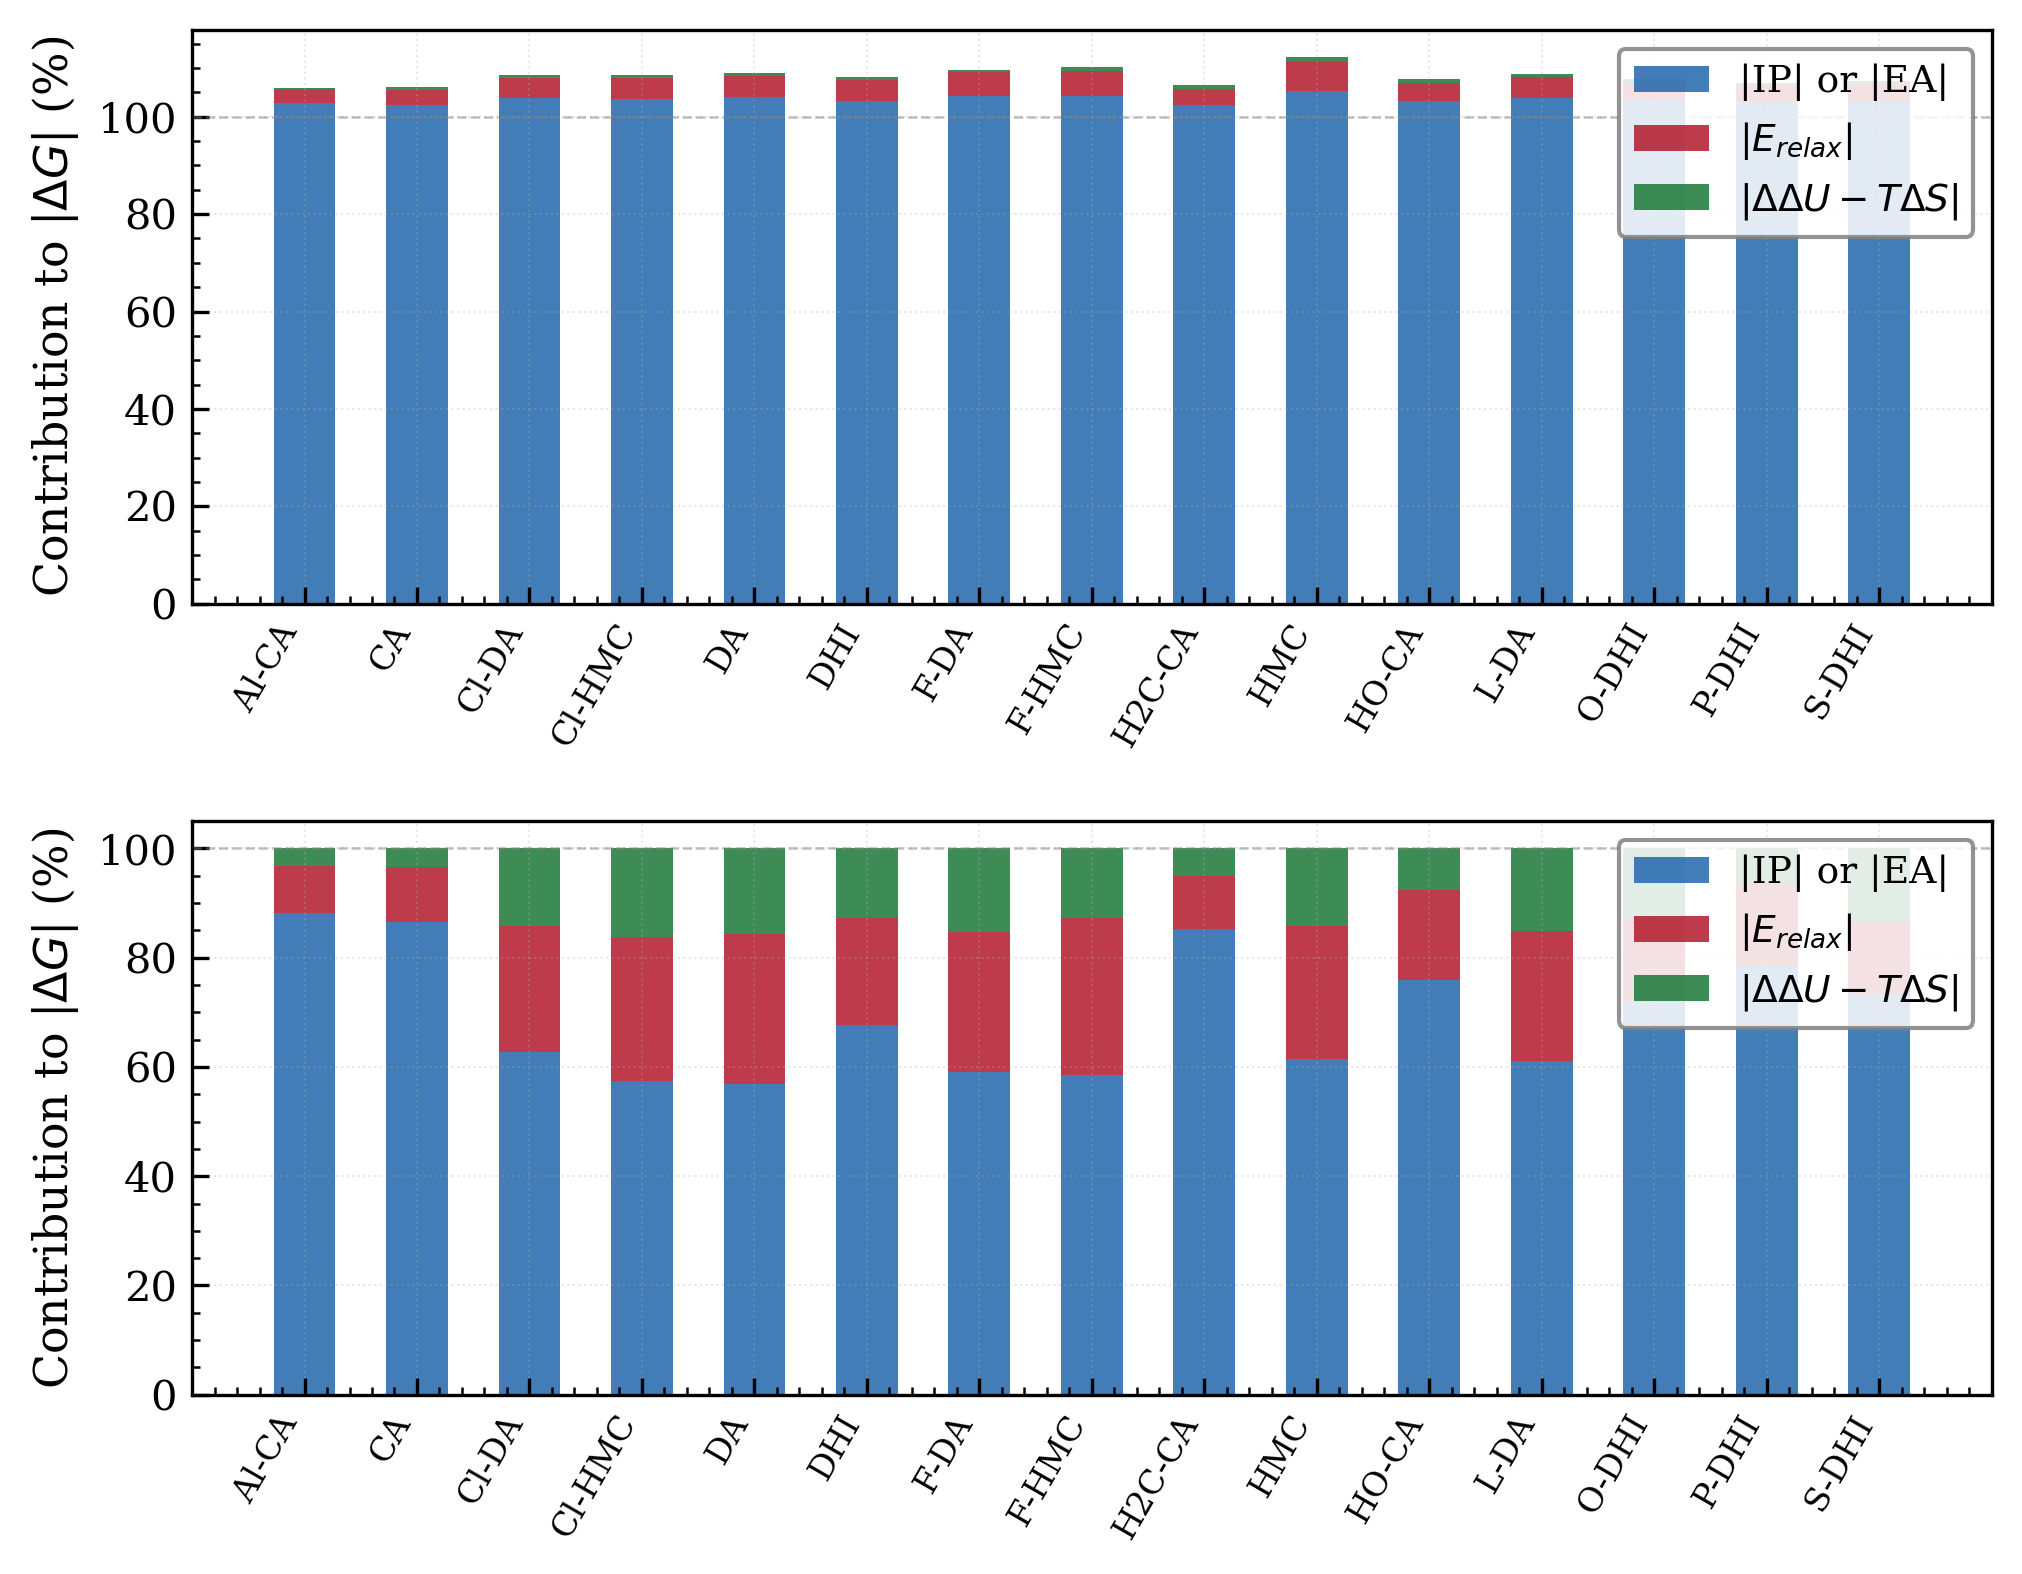
\includegraphics[width=0.85\textwidth]{decomposition_magnitude_bars.png}
\caption{Décomposition de $|\Delta G|$ en contributions. Barres empilées : IP ou EA (bleu), $|E_{\text{relax}}|$ (rouge), $|\Delta\Delta U - T\Delta S|$ (vert). En oxydation, IP domine uniformément ; en réduction, la répartition varie selon la molécule.}
\label{fig:decomp_bars}
\end{figure}

\subsection{Corrélations EA/IP avec les Orbitales Frontières}

\subsubsection{Théorème de Koopmans}
\label{sec:koopmans}

Le théorème de Koopmans (1934)~\cite{koopmans1934} établit, dans le cadre Hartree-Fock, que le potentiel d'ionisation vertical d'un système à $N$ électrons est égal à l'opposé de l'énergie de l'orbitale HOMO : $\text{IP} = -\varepsilon_{\text{HOMO}}$. Cette égalité repose sur l'hypothèse que les orbitales ne se réorganisent pas lors du retrait d'un électron (\emph{frozen orbital approximation}), négligeant ainsi l'énergie de relaxation orbitale et la corrélation électronique. Pour l'affinité électronique, la correspondance $\text{EA} \approx -\varepsilon_{\text{LUMO}}$ est moins rigoureuse en Hartree-Fock. En effet, les orbitales HF sont optimisées variationnellement pour l'état fondamental à $N$ électrons : la HOMO fait partie de cet ensemble optimal, ce qui fonde la relation IP $= -\varepsilon_{\text{HOMO}}$. La LUMO, en revanche, est une orbitale \emph{virtuelle} qui émerge de la résolution des équations HF sans avoir jamais été occupée. Pour décrire correctement le système à $N+1$ électrons (l'anion), il faudrait ré-optimiser l'ensemble des orbitales en présence de l'électron supplémentaire, ce qui donnerait des orbitales significativement différentes. La LUMO du système à $N$ électrons n'est donc qu'une approximation de l'orbitale qu'occuperait réellement l'électron ajouté, et le théorème de Koopmans au sens strict ne concerne que l'ionisation.

En théorie de la fonctionnelle de la densité (DFT) de Kohn-Sham, la situation est différente. Le théorème de Janak~\cite{janak1978} garantit que, pour la fonctionnelle exacte, $-\varepsilon_{\text{HOMO}}^{\text{KS}}$ est rigoureusement égal au potentiel d'ionisation exact. Cependant, avec des fonctionnelles approchées comme PBE0, les énergies orbitales de Kohn-Sham souffrent de l'erreur de self-interaction résiduelle, et la correspondance n'est qu'approximative. On parle donc d'\emph{approximation} de Koopmans plutôt que de théorème au sens strict. Malgré ces limitations, une corrélation linéaire empirique entre les énergies orbitalaires KS ($\varepsilon_{\text{HOMO}}$, $\varepsilon_{\text{LUMO}}$) et les énergies verticales (IP, EA) est largement documentée dans la littérature et constitue un outil de criblage rapide.

La figure~\ref{fig:koopmans} montre les corrélations obtenues sur notre série de catéchols entre les énergies orbitalaires de Kohn-Sham et les énergies verticales calculées par DFT (schéma composite TZ2P). Pour IP vs $-\varepsilon_{\text{HOMO}}$ (figure~\ref{fig:koopmans_ip_filtered}), la corrélation est très bonne ($R^2 = 0.974$, MAE $= \SI{2.1}{kJ/mol}$, $n = 15$). Pour EA vs $-\varepsilon_{\text{LUMO}}$ (figure~\ref{fig:koopmans_ea_filtered}), la corrélation est excellente ($R^2 = 0.998$, MAE $= \SI{2.3}{kJ/mol}$, $n = 15$). L'analyse per-conformère, où chaque conformère constitue un point indépendant ($n = 40$), confirme ces corrélations avec une puissance statistique accrue (figure~\ref{fig:koopmans}c--d).

Ces MAE de l'ordre de \SI{2}{kJ/mol} sont remarquablement faibles et comparables à l'erreur intrinsèque de la fonctionnelle PBE0, typiquement estimée à \SIrange{4}{8}{kJ/mol} (1--2~kcal/mol) sur les énergies de réaction. Koopmans atteint donc la limite de précision du calcul de référence lui-même pour cette série. La qualité de ces corrélations s'explique par l'homogénéité chimique de notre jeu de données : tous les composés partagent le squelette catéchol/quinone, et les variations de substituants modifient les niveaux orbitalaires de manière continue et monotone. La dispersion résiduelle per-conformère provient principalement de la variabilité du terme $E_{\text{relax}}$, qui n'est pas capturé par l'approximation de Koopmans, et non d'un échec de la corrélation orbitalaire elle-même. Cette observation motive l'exploration de modèles au-delà de l'orbitale frontière unique.

\begin{figure}[H]
\centering
\begin{subfigure}[t]{0.42\textwidth}
\centering
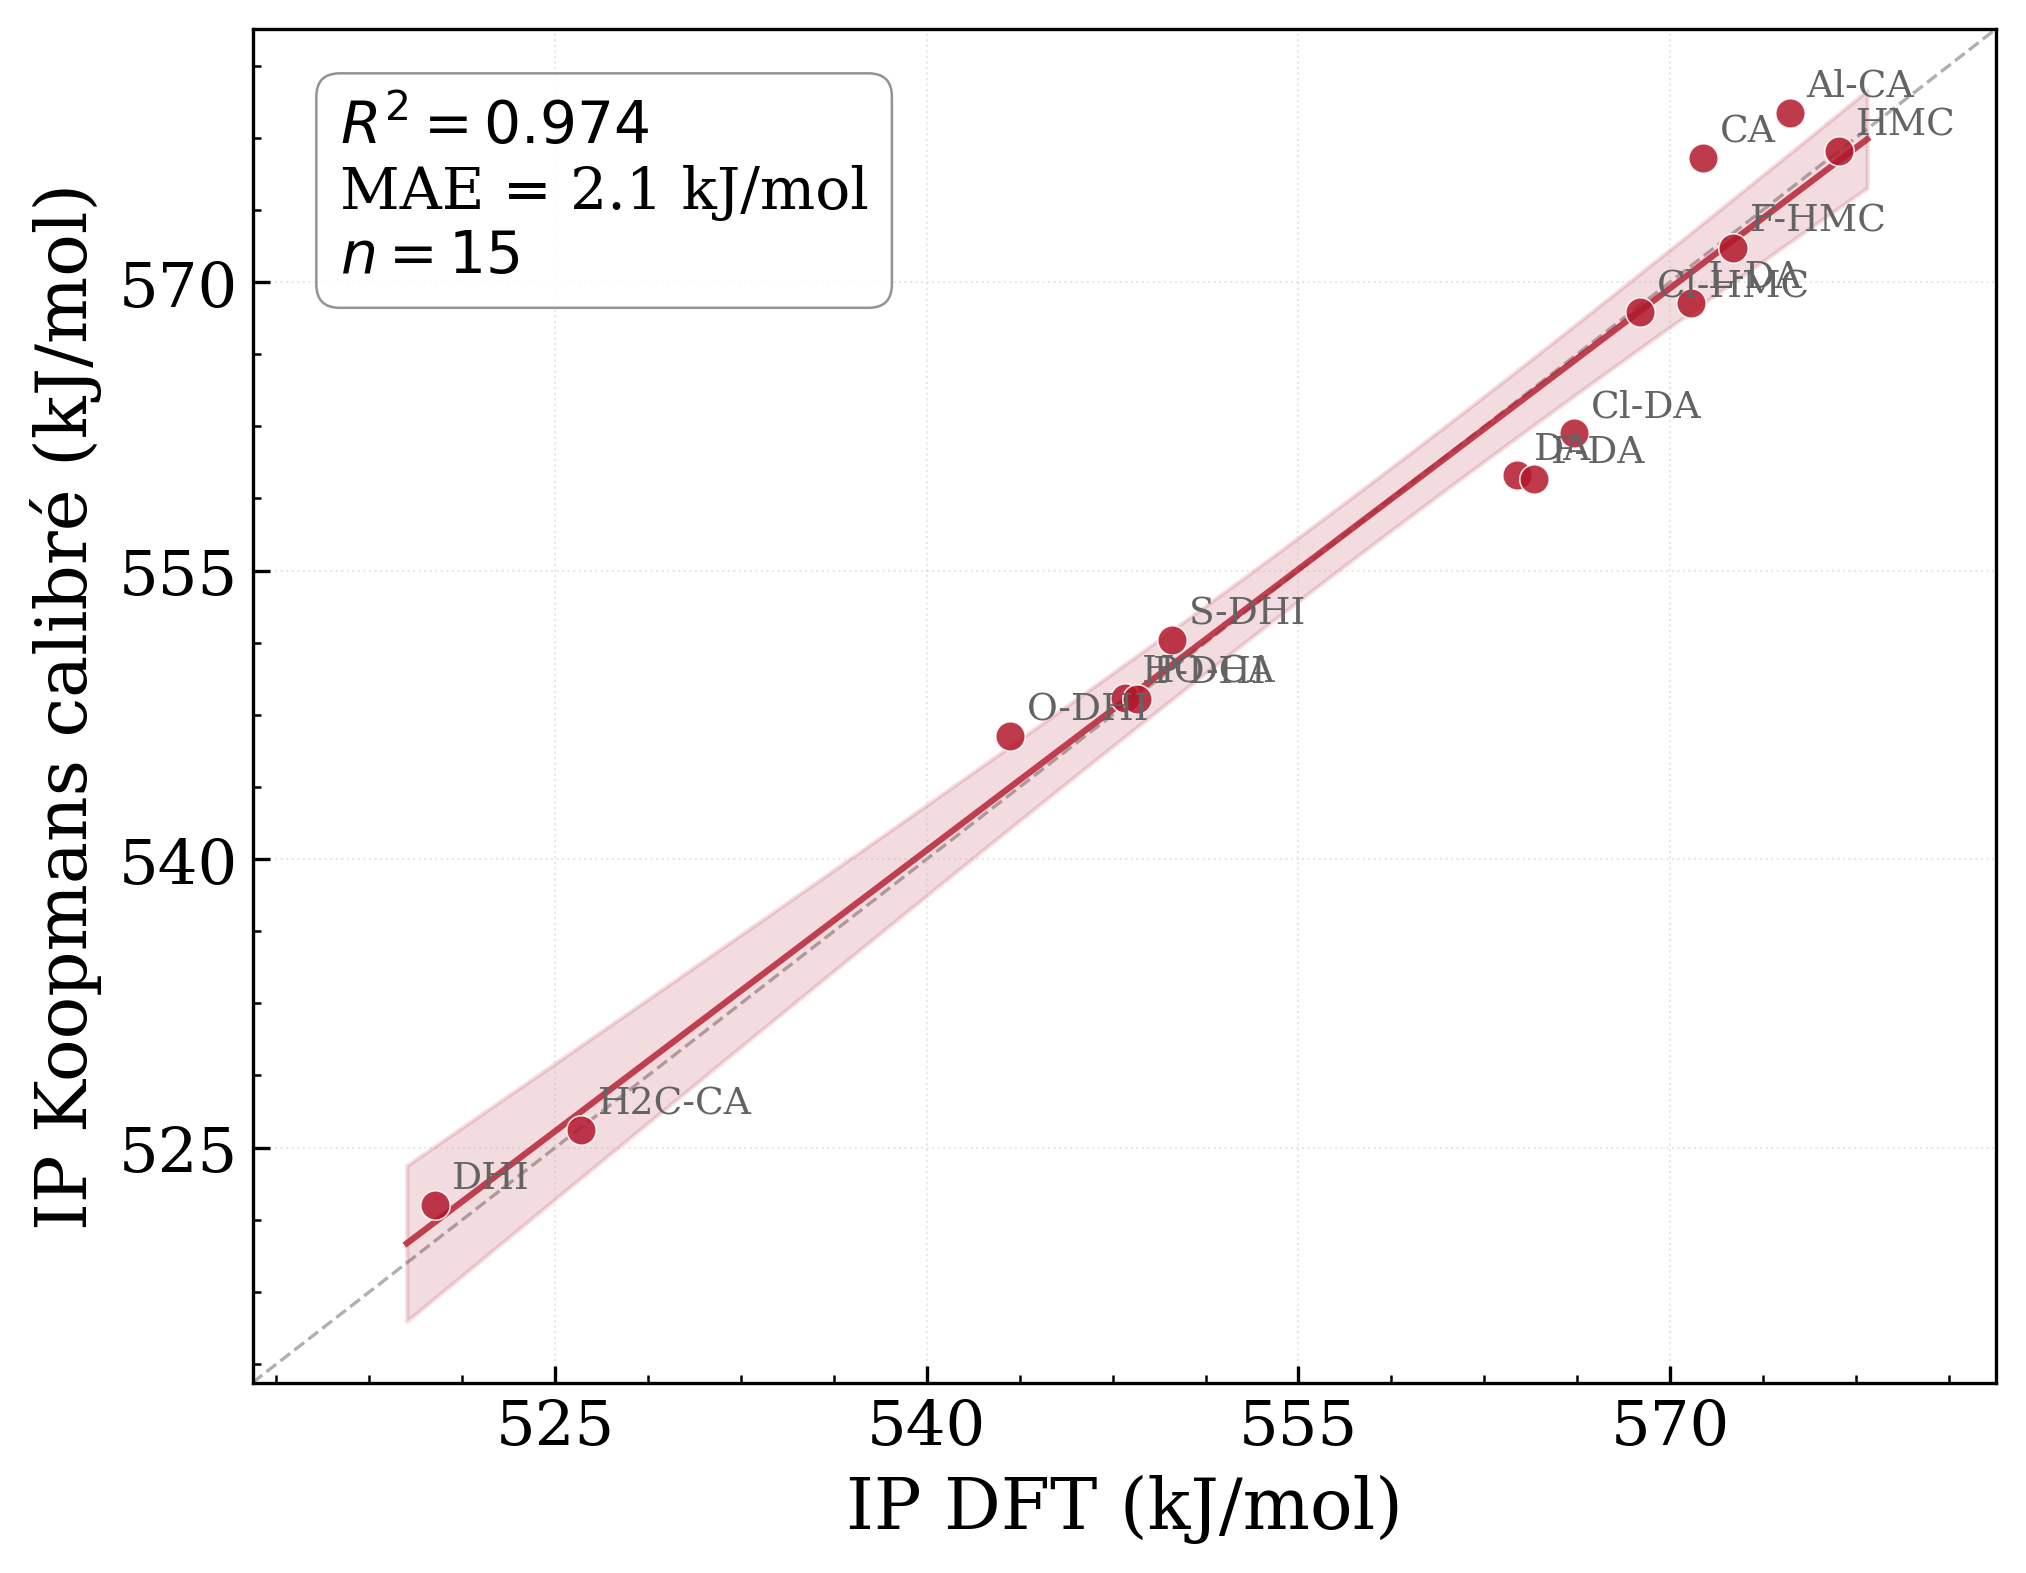
\includegraphics[width=\textwidth]{IP_vs_HOMO_sans_outliers.png}
\caption{IP vs HOMO ($R^2 = 0.974$, $n=15$).}
\label{fig:koopmans_ip_filtered}
\end{subfigure}
\hfill
\begin{subfigure}[t]{0.42\textwidth}
\centering
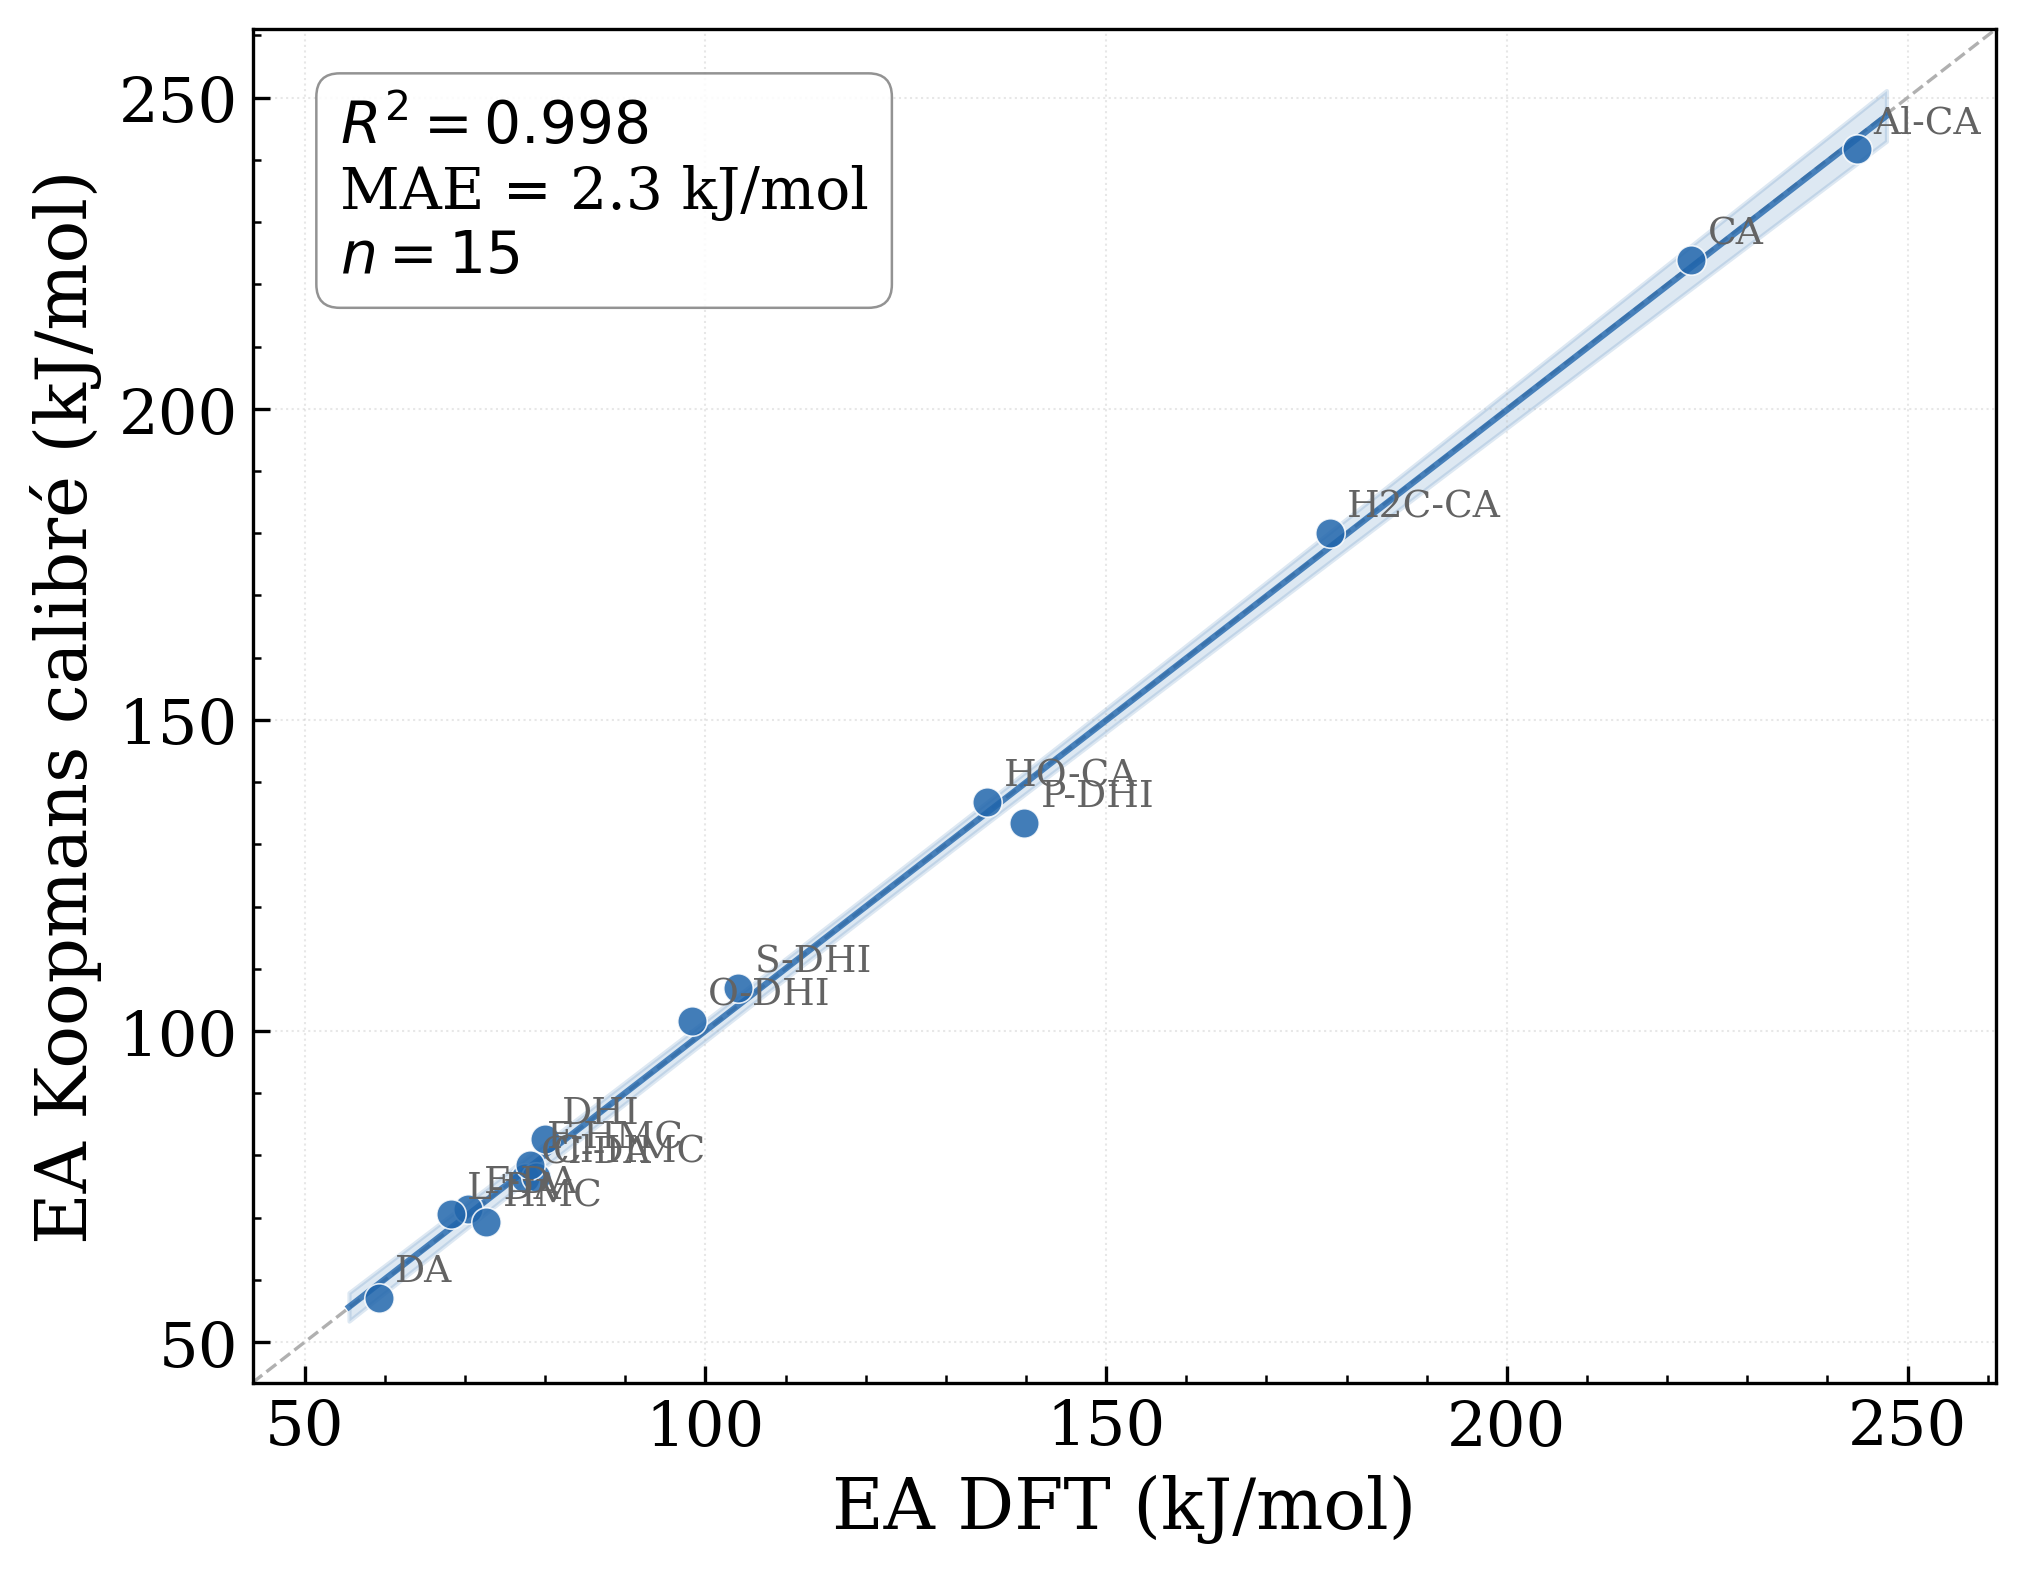
\includegraphics[width=\textwidth]{EA_vs_LUMO_sans_outliers.png}
\caption{EA vs LUMO ($R^2 = 0.998$, $n=15$).}
\label{fig:koopmans_ea_filtered}
\end{subfigure}

\vspace{4pt}
\begin{subfigure}[t]{0.42\textwidth}
\centering
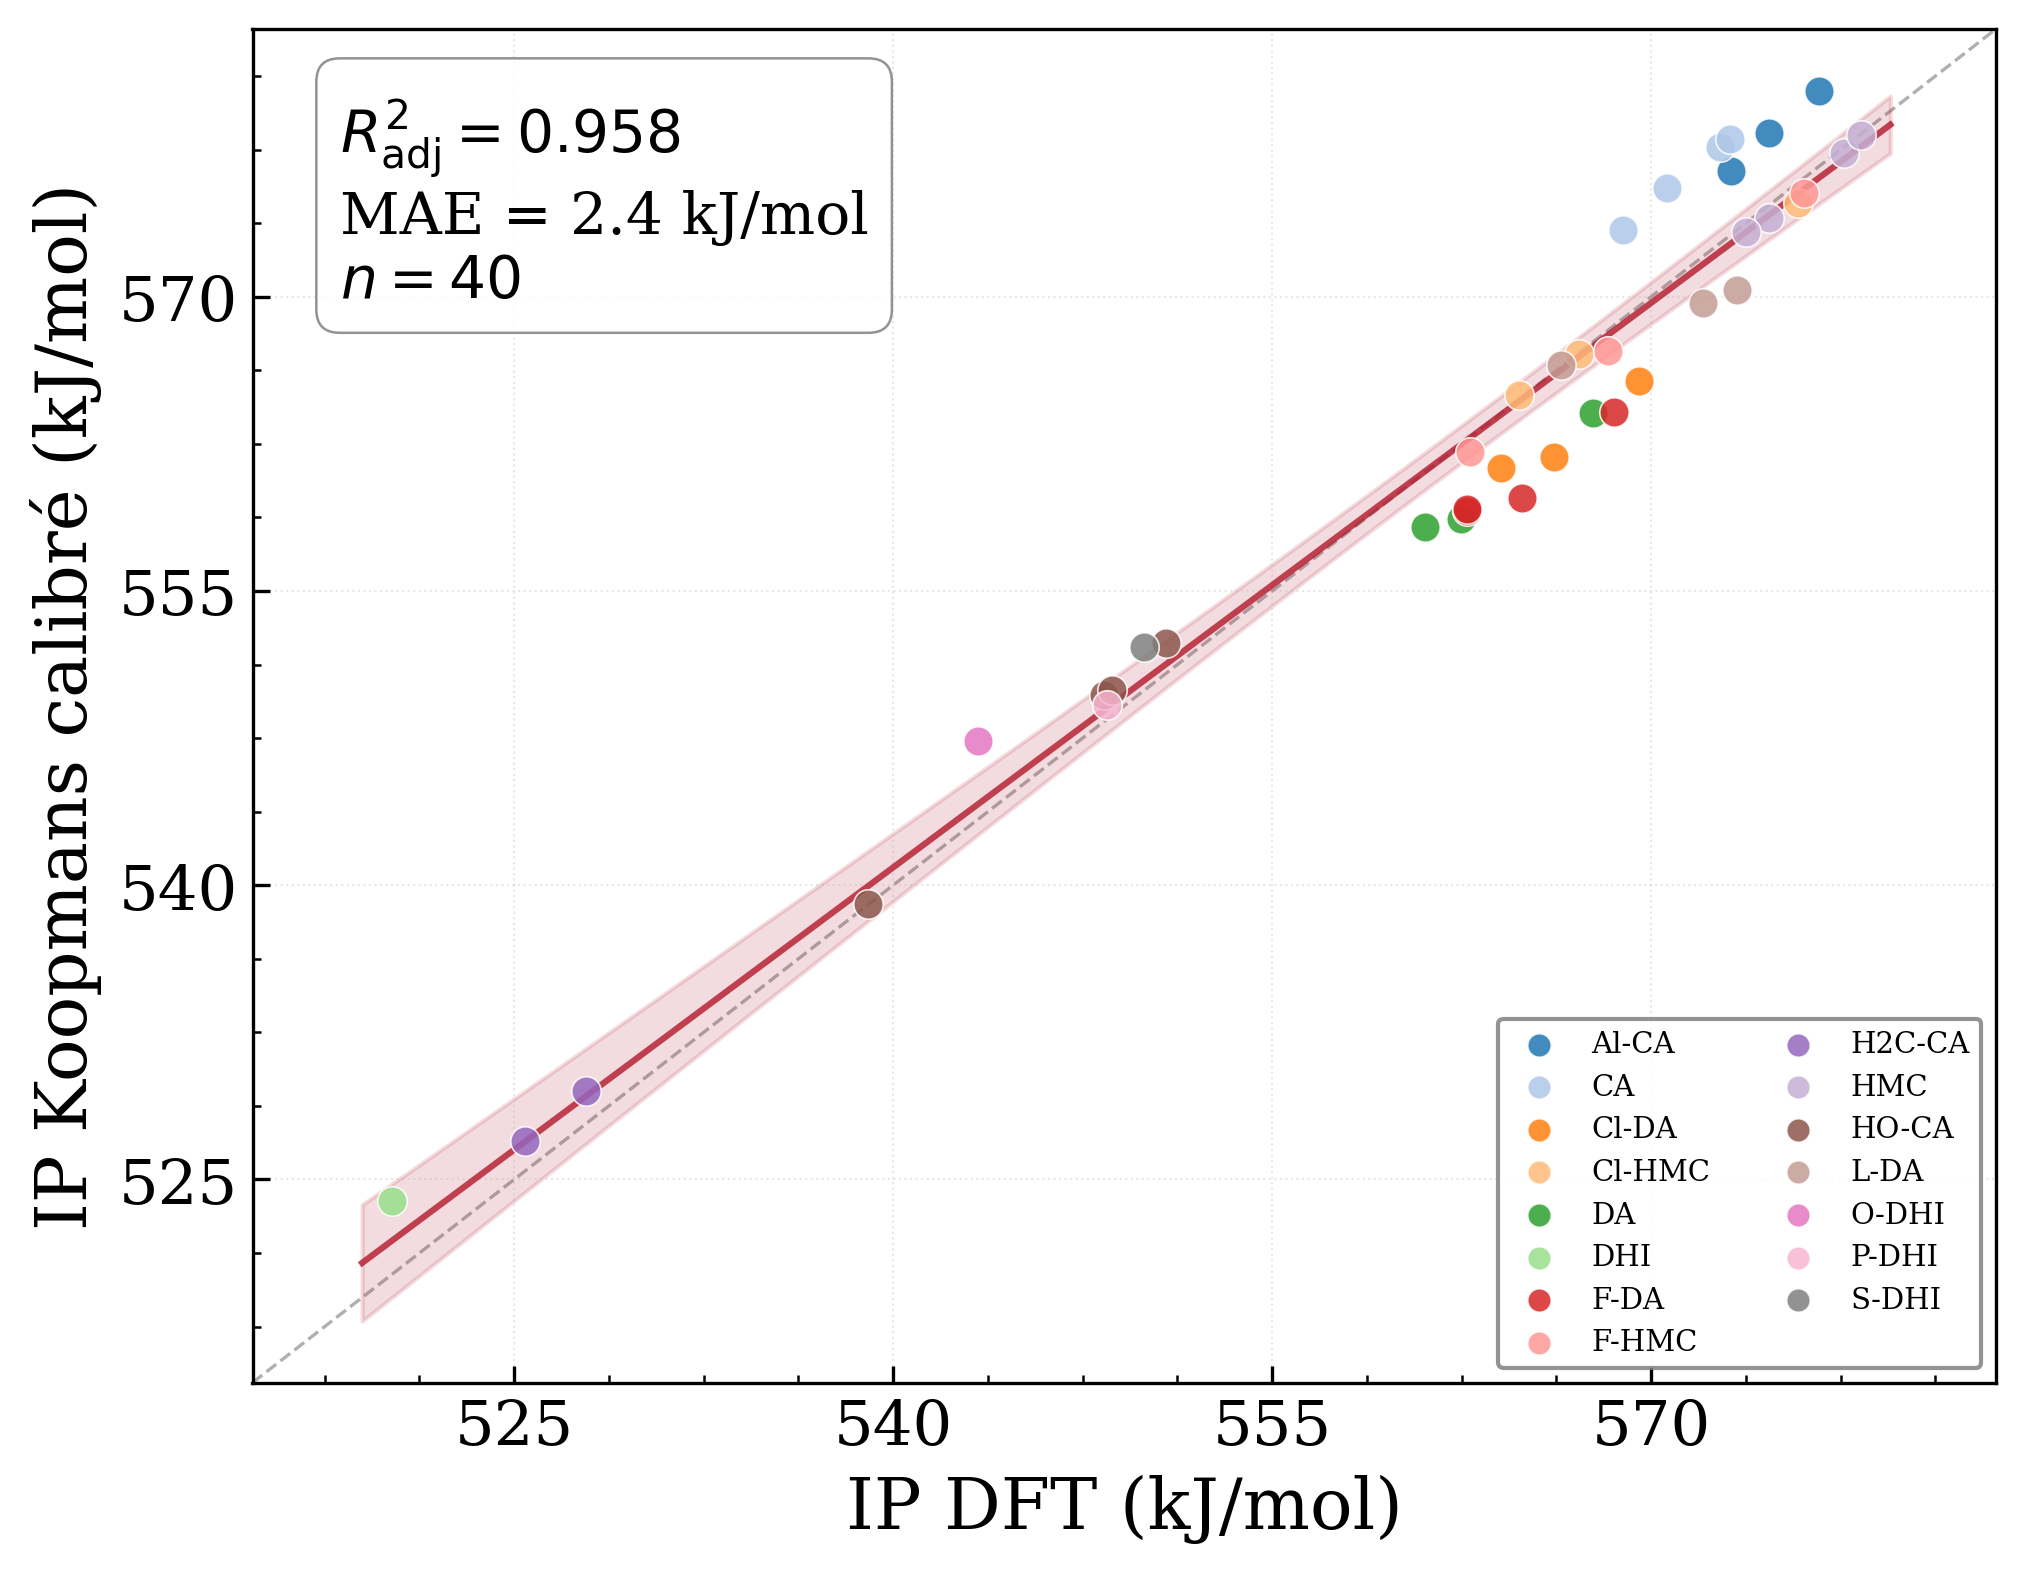
\includegraphics[width=\textwidth]{IP_vs_HOMO_per_conformer_sans_outliers.png}
\caption{IP vs HOMO per-conformère ($R^2_{\text{adj}} = 0.958$, $n = 40$).}
\label{fig:koopmans_ip_pc_filt}
\end{subfigure}
\hfill
\begin{subfigure}[t]{0.42\textwidth}
\centering
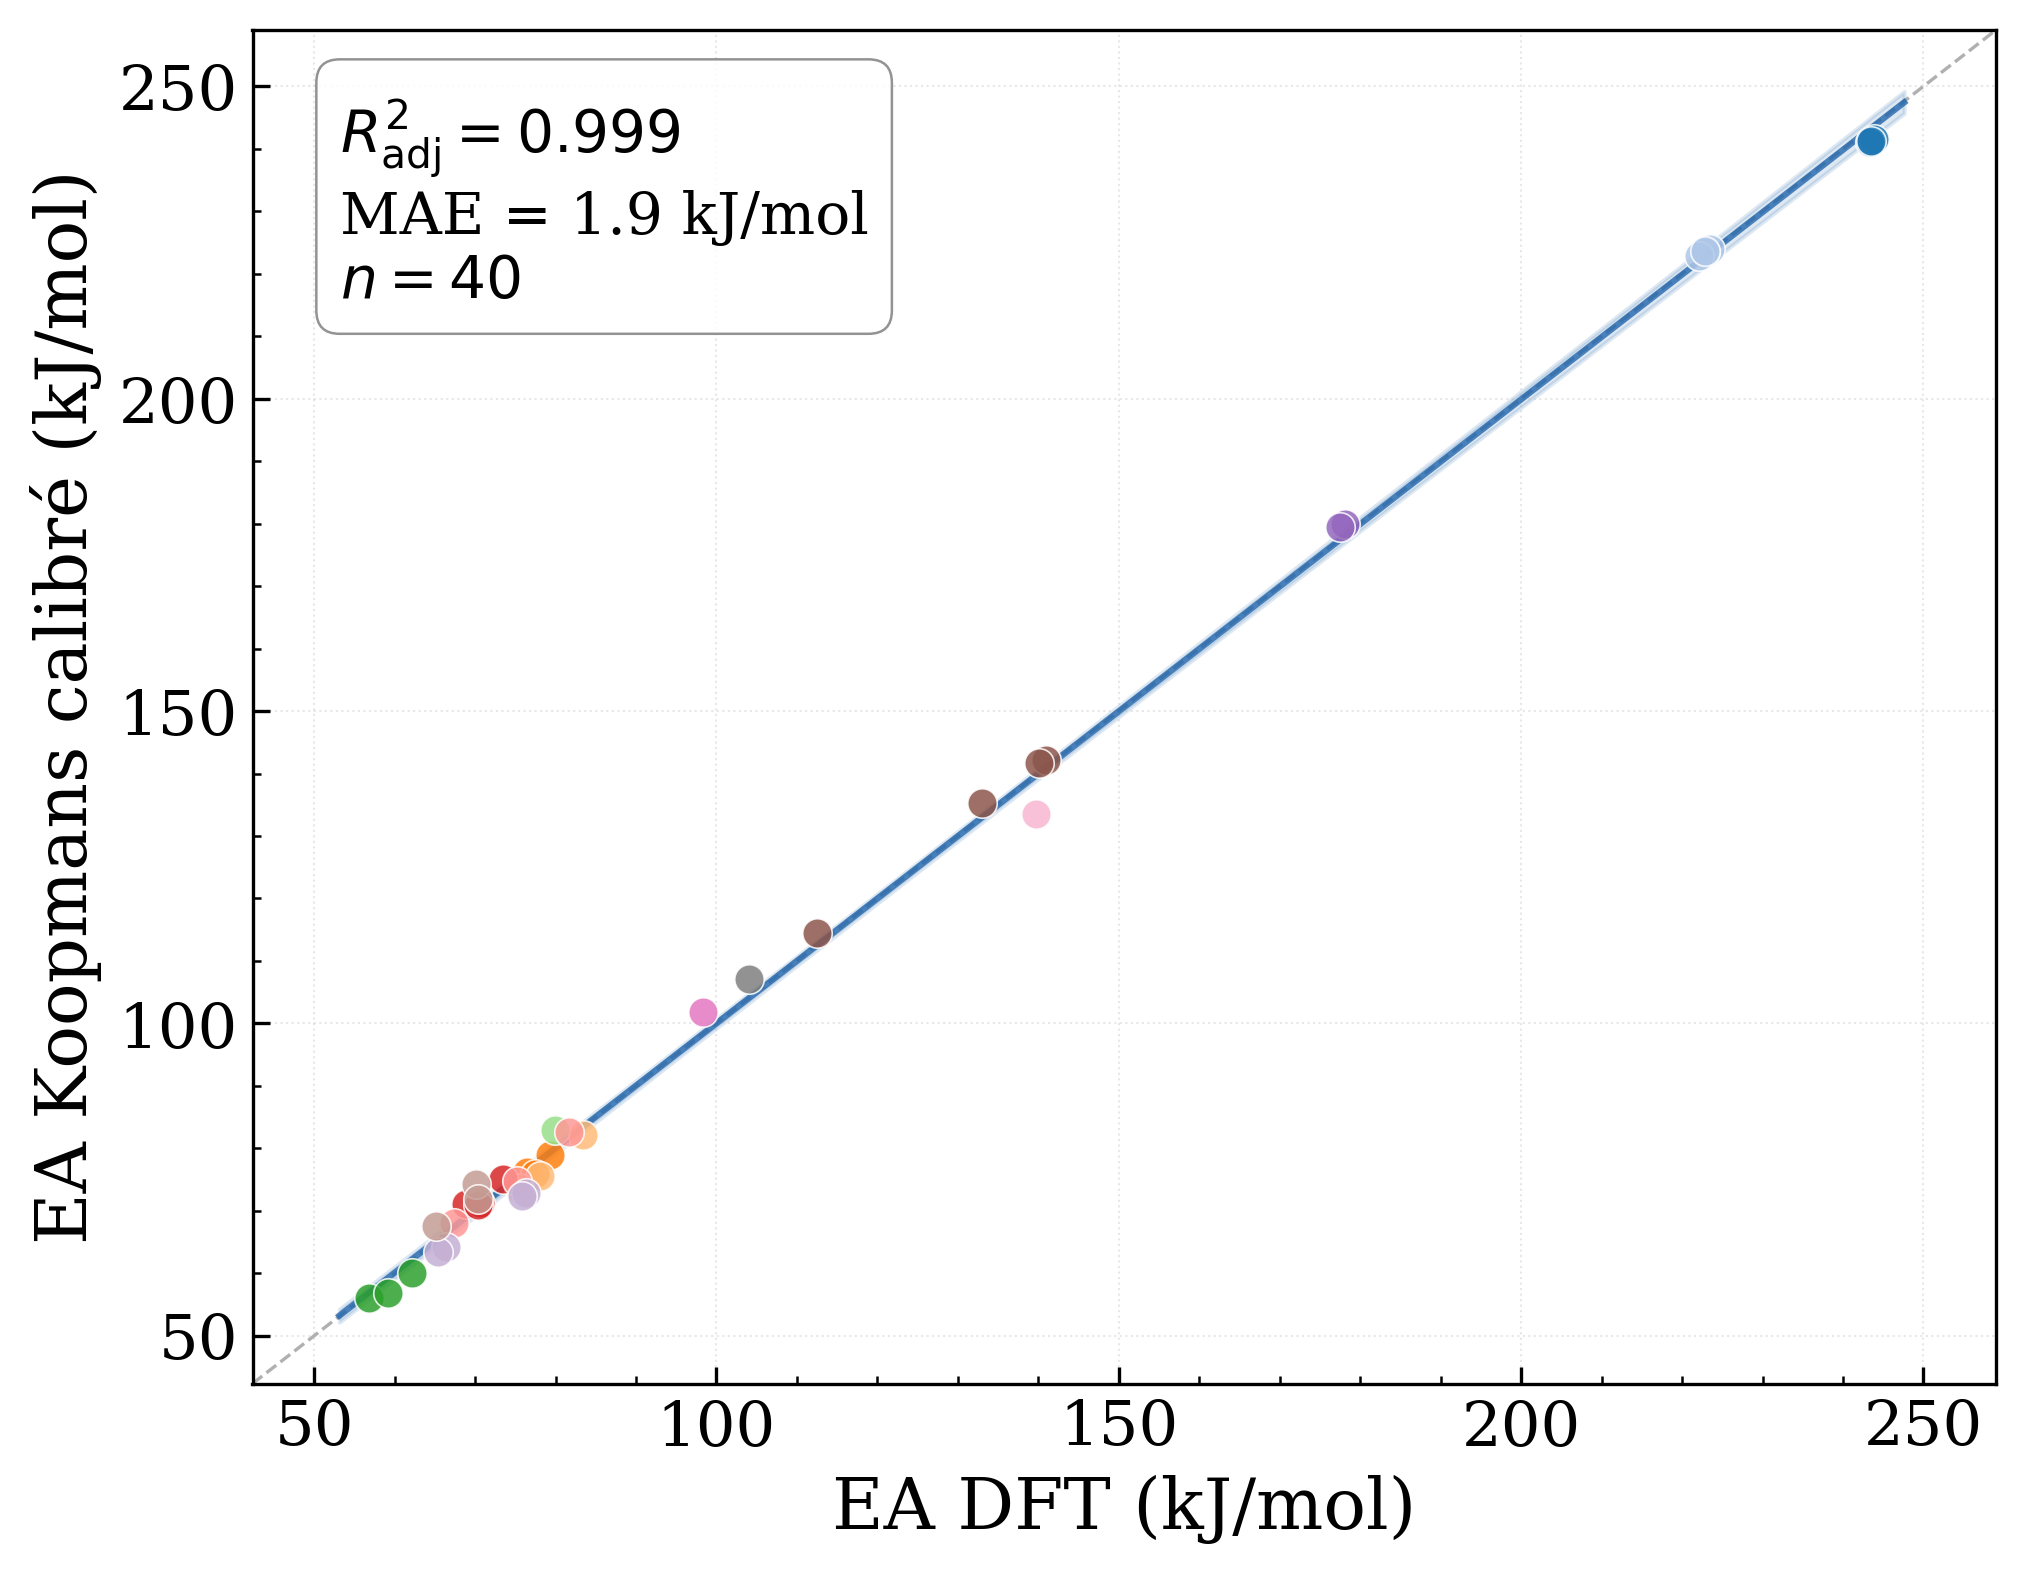
\includegraphics[width=\textwidth]{EA_vs_LUMO_per_conformer_sans_outliers.png}
\caption{EA vs LUMO per-conformère ($R^2_{\text{adj}} = 0.999$, $n = 40$).}
\label{fig:koopmans_ea_pc_filt}
\end{subfigure}
\caption{Corrélations de Koopmans (schéma composite TZ2P). (a)--(b) Moyennes de Boltzmann par molécule ($n = 15$). (c)--(d) Per-conformère (couleurs par molécule, $n = 40$).}
\label{fig:koopmans}
\end{figure}

\subsubsection{Au-delà de Koopmans : l'approche de Politzer et Murray}
\label{sec:politzer}

L'approximation de Koopmans repose sur une seule orbitale frontière (HOMO ou LUMO), négligeant la contribution de toutes les autres orbitales à la densité électronique. L'énergie d'ionisation locale moyenne (\emph{Average Local Ionization Energy}, ALIE), introduite par Politzer et Murray~\cite{politzer2010}, propose une approche \emph{a priori} plus complète en intégrant la contribution de l'ensemble des orbitales occupées à la densité locale. Cette formulation devrait en principe mieux capturer les effets de délocalisation et de structure électronique profonde qui influencent le potentiel d'ionisation. L'ALIE en un point $\mathbf{r}$ est définie par :
\begin{equation}
\bar{I}(\mathbf{r}) = \frac{\sum_i n_i \, |\psi_i(\mathbf{r})|^2 \, |\varepsilon_i|}{\rho(\mathbf{r})}
\label{eq:alie}
\end{equation}
où $n_i$ est l'occupation, $\psi_i(\mathbf{r})$ la fonction d'onde et $\varepsilon_i$ l'énergie de l'orbitale $i$, et $\rho(\mathbf{r})$ la densité électronique totale. L'ALIE représente ainsi l'énergie moyenne nécessaire pour arracher un électron au point $\mathbf{r}$, pondérée par la contribution de chaque orbitale à la densité locale.

Le descripteur clé est $\bar{I}_{S,\min}$, la valeur minimale de l'ALIE sur la surface d'isodensité $\rho = \SI{0.001}{a.u.}$ Cette surface, qui correspond approximativement à l'enveloppe de van der Waals de la molécule, est le lieu où les interactions intermoléculaires débutent. Le minimum $\bar{I}_{S,\min}$ identifie le site où les électrons sont les plus faiblement liés et corrèle linéairement avec le potentiel d'ionisation vertical pour des séries de molécules apparentées~\cite{politzer2010}. De façon analogue, le minimum du potentiel électrostatique sur cette même surface ($V_{S,\min}$) est relié à l'affinité électronique.

\paragraph{Implémentation.}
Nous avons implémenté le calcul de l'ALIE par post-traitement DENSF sur les fichiers RKF des calculs neutres existants, sans nouveau calcul SCF. Le pipeline comprend quatre phases : (i)~calcul de la densité SCF sur une grille 3D, (ii)~extraction des points de l'isosurface $\rho = \SI{0.001}{a.u.}$ par interpolation linéaire sur les arêtes de la grille ($\sim$25\,000 points par molécule), (iii)~évaluation des orbitales occupées, de la densité et du potentiel coulombien à chaque point de surface via DENSF en mode \texttt{Grid Inline}, et (iv)~calcul de $\bar{I}(\mathbf{r})$ selon l'équation~\eqref{eq:alie} et extraction des descripteurs $\bar{I}_{S,\min}$ et $V_{S,\min}$.

\paragraph{Résultats.}
L'analyse a été réalisée sur 34 molécules (catéchols et quinones) totalisant 74 conformères. Les valeurs de $\bar{I}_{S,\min}$ obtenues se situent entre \SIrange{7.8}{9.9}{eV}, dans la gamme attendue pour des molécules organiques. Cependant, après calibration par régression linéaire (figure~\ref{fig:politzer}), les erreurs de prédiction restent élevées : MAE $= \SI{49.6}{kJ/mol}$ pour $\bar{I}_{S,\min}$ vs IP ($R^2 = 0.10$) et MAE $= \SI{56.0}{kJ/mol}$ pour $-V_{S,\min}$ vs EA ($R^2 = 0.76$). En comparaison, l'approximation de Koopmans donne MAE $= \SI{2.1}{kJ/mol}$ pour IP ($R^2 = 0.974$) et MAE $= \SI{2.3}{kJ/mol}$ pour EA ($R^2 = 0.998$).

\begin{figure}[H]
\centering
\begin{subfigure}[t]{0.42\textwidth}
\centering
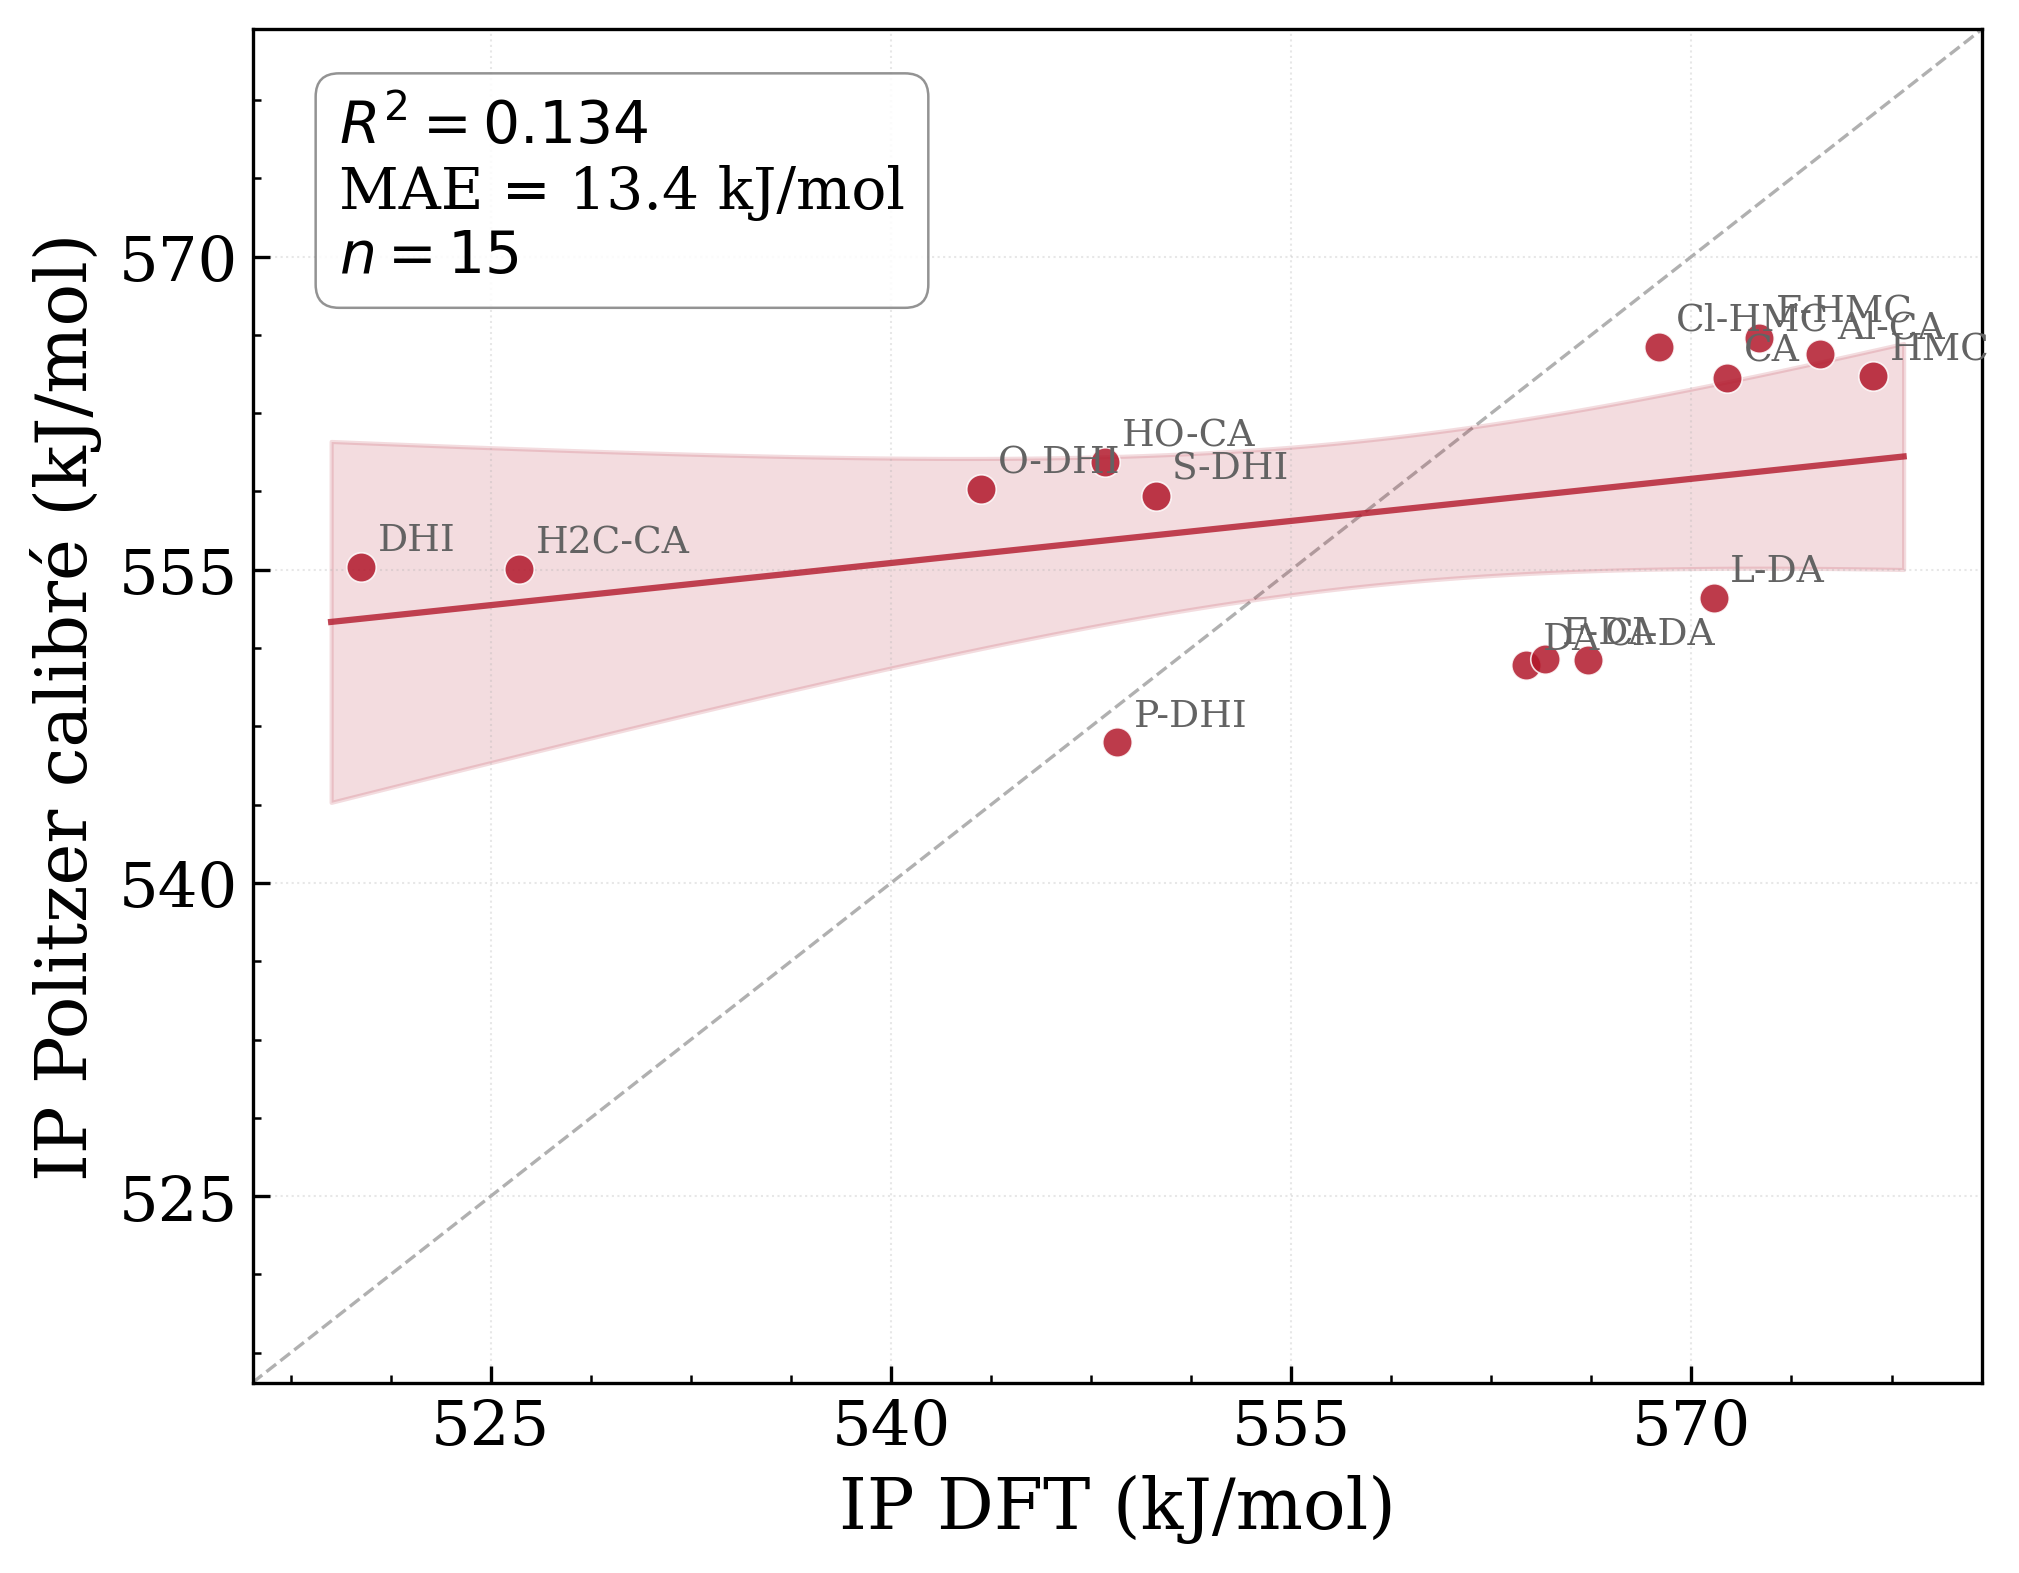
\includegraphics[width=\textwidth]{politzer/IP_Politzer_per_molecule.png}
\caption{IP Politzer calibré ($n = 15$).}
\label{fig:politzer_ip_pol}
\end{subfigure}
\hfill
\begin{subfigure}[t]{0.42\textwidth}
\centering
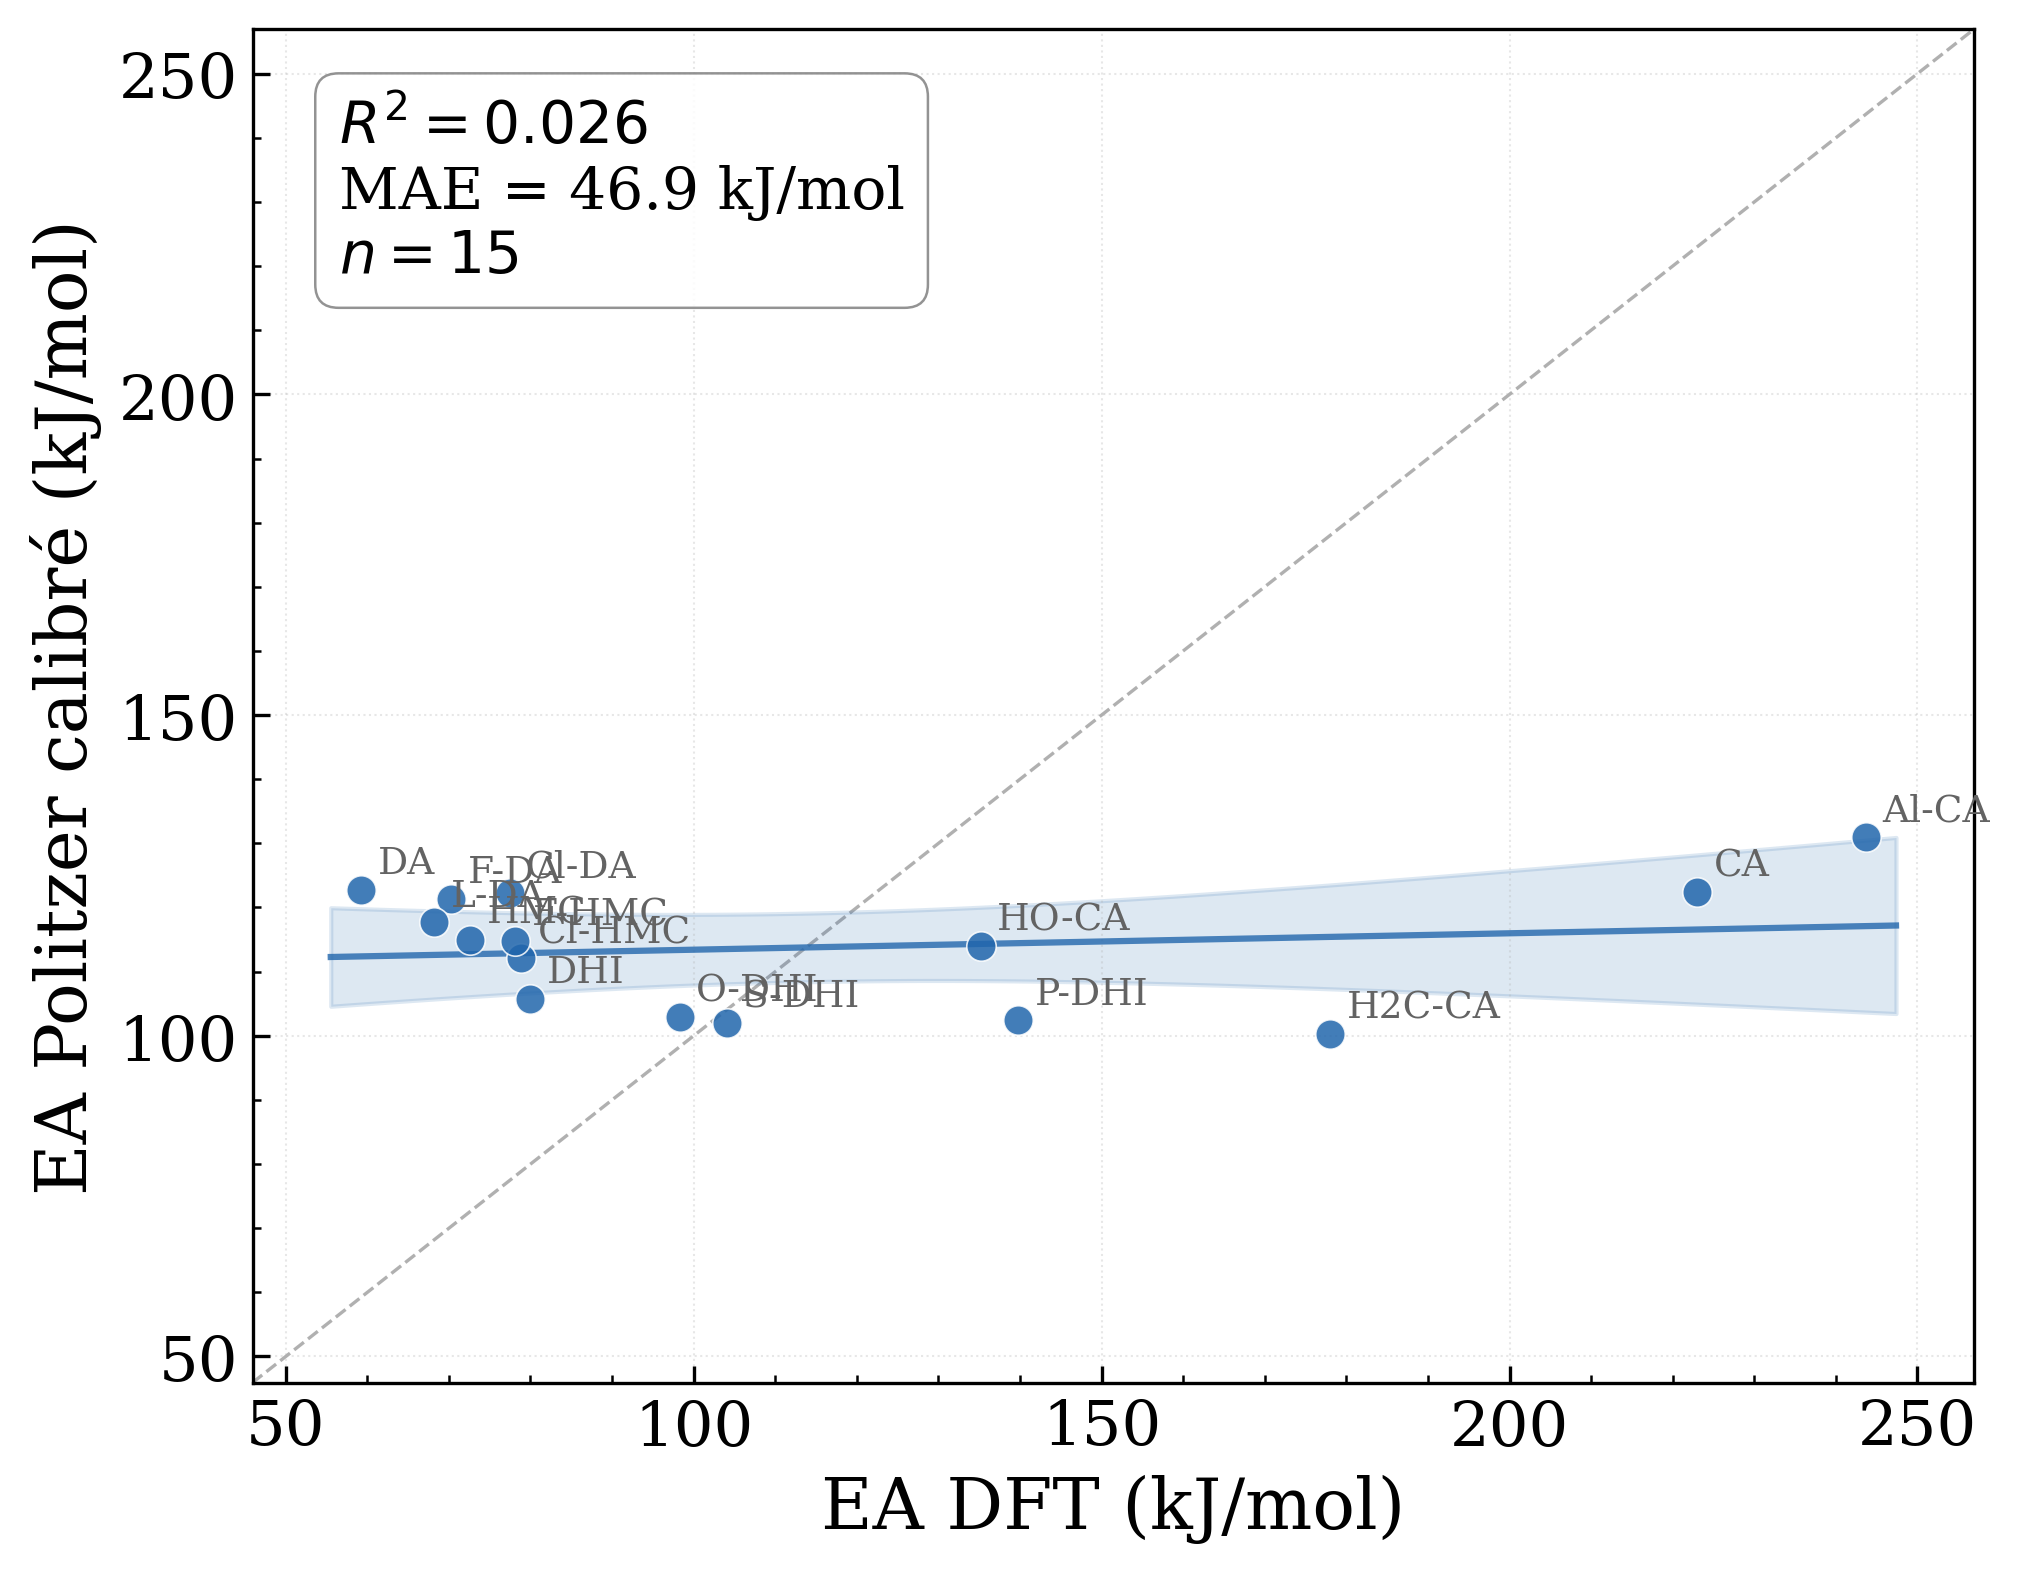
\includegraphics[width=\textwidth]{politzer/EA_Politzer_per_molecule.png}
\caption{EA Politzer calibré ($n = 15$).}
\label{fig:politzer_ea_pol}
\end{subfigure}

\vspace{4pt}
\begin{subfigure}[t]{0.42\textwidth}
\centering
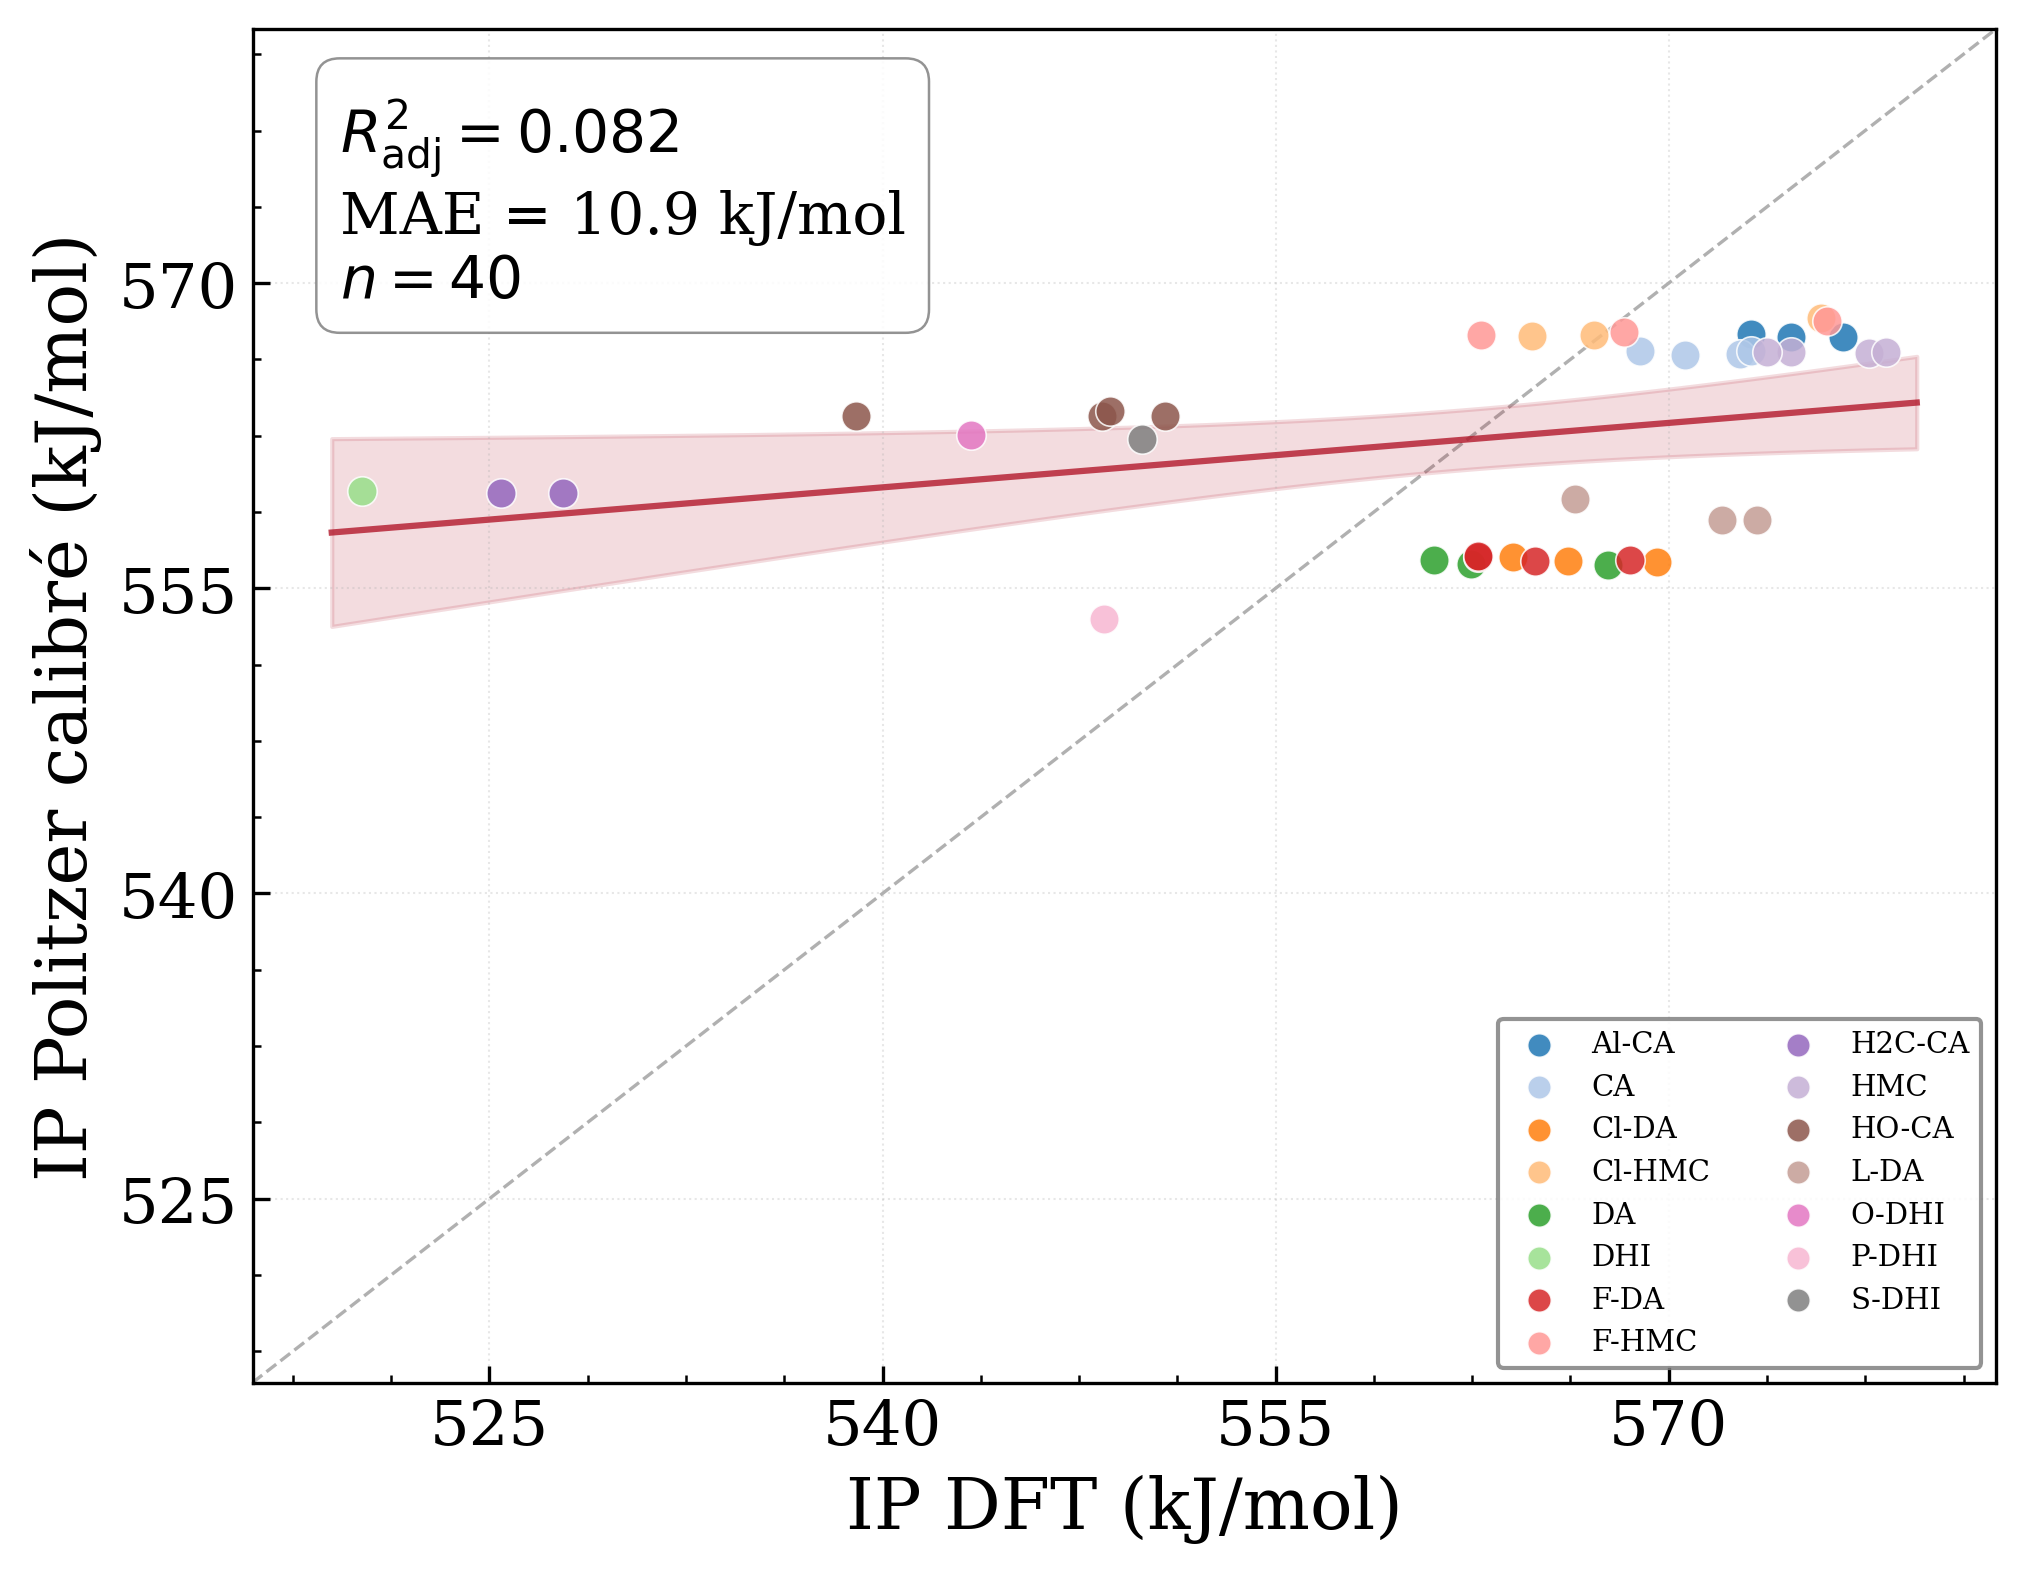
\includegraphics[width=\textwidth]{politzer/IP_vs_ALIE_per_conformer.png}
\caption{IP vs $\bar{I}_{S,\min}$ per-conformère ($n = 40$).}
\label{fig:politzer_ip_pc}
\end{subfigure}
\hfill
\begin{subfigure}[t]{0.42\textwidth}
\centering
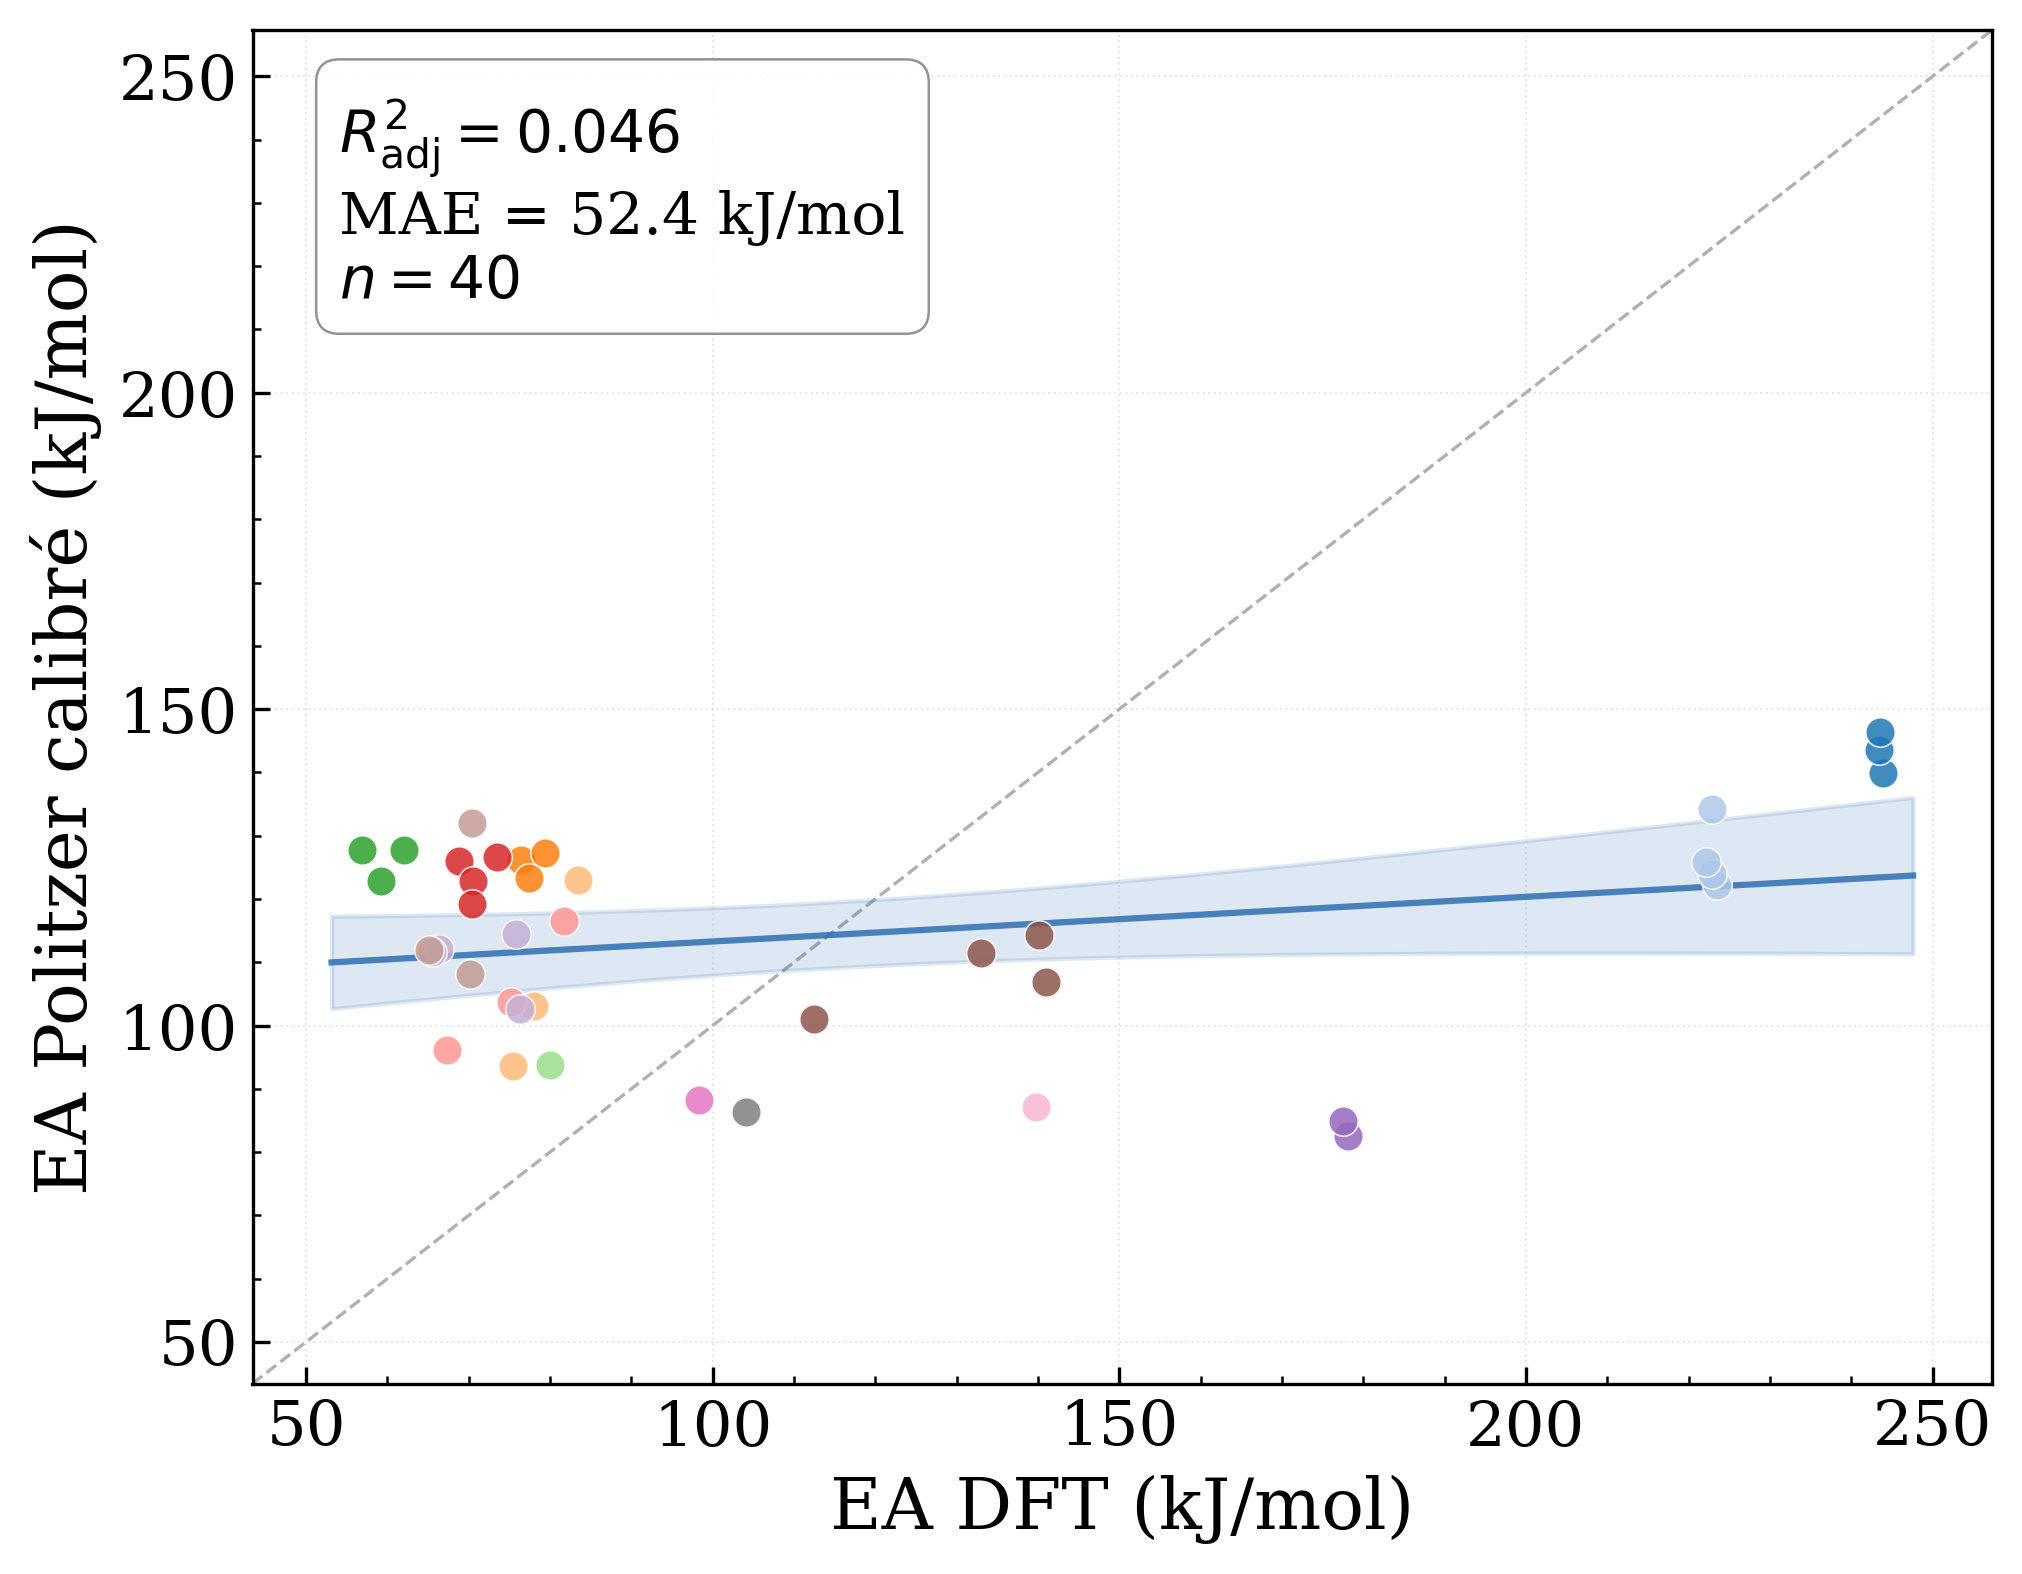
\includegraphics[width=\textwidth]{politzer/EA_vs_VS_per_conformer.png}
\caption{EA vs $-V_{S,\min}$ per-conformère ($n = 40$).}
\label{fig:politzer_ea_pc}
\end{subfigure}
\caption{Prédictions Politzer calibrées ($\bar{I}_{S,\min}$, $-V_{S,\min}$). (a)--(b) Par molécule. (c)--(d) Per-conformère (couleurs par molécule). À comparer avec les corrélations de Koopmans (figure~\ref{fig:koopmans}).}
\label{fig:politzer}
\end{figure}

L'analyse per-conformère (figure~\ref{fig:politzer}c--d) confirme l'absence de pouvoir prédictif de Politzer. Le contraste avec Koopmans per-conformère (figure~\ref{fig:koopmans}c--d) est saisissant.

\paragraph{Analyse de l'échec.}
Ces résultats sont étonnamment mauvais. Dans la littérature, Politzer et Murray rapportent des corrélations $R^2 > 0.93$ pour $\bar{I}_{S,\min}$ vs IP au sein de séries homologues (benzènes substitués, azines), et même sur des séries moléculaires diversifiées, $R^2$ reste typiquement supérieur à 0.70~\cite{politzer2010}. Notre série de catéchols, chimiquement homogène (même squelette, variations de substituants modérées), devrait \emph{a priori} donner des résultats au moins comparables. L'obtention d'un $R^2 = 0.10$ pour l'IP suggère un problème d'implémentation plutôt qu'une limitation intrinsèque de la méthode.

Une analyse rétrospective de notre code a en effet révélé plusieurs limitations. Premièrement, le descripteur $V_{S,\min}$ a été calculé à partir du potentiel coulombien électronique seul (\texttt{POTENTIAL coul SCF} dans DENSF), et non du potentiel électrostatique moléculaire total (MEP $= V_{\text{nucléaire}} + V_{\text{électronique}}$) tel que défini par Politzer et Murray. Cela invalide la comparaison avec la littérature pour l'EA. Deuxièmement, des problèmes de robustesse ont été identifiés lors de la réutilisation de fichiers TAPE41 pré-existants, pouvant conduire à des résultats corrompus sur certains conformères. Enfin, la résolution de la grille utilisée (\texttt{GRID medium}) pourrait être insuffisante pour localiser précisément le minimum global de $\bar{I}(\mathbf{r})$ sur l'isosurface.

En l'état, nous ne pouvons pas conclure sur la validité de l'approche de Politzer pour notre système. Cette piste nécessite une révision de l'implémentation --- en particulier l'utilisation du MEP total pour $V_{S,\min}$ et la vérification de l'intégrité des données de surface --- avant de pouvoir être comparée équitablement à l'approximation de Koopmans, qui reste le prédicteur le plus fiable avec des MAE de \SIrange{1.9}{2.4}{kJ/mol}. L'approche de Politzer, même correctement implémentée, resterait cependant un outil complémentaire : elle donne accès à une information \emph{spatiale} (le site le plus réactif) que les énergies orbitales seules ne fournissent pas. La section suivante explore une voie intermédiaire entre Koopmans (une seule orbitale) et Politzer (toutes les orbitales) en restreignant les descripteurs aux quelques orbitales voisines des frontières.

\subsubsection{Régression multi-orbitale : au-delà de l'orbitale frontière unique}
\label{sec:multi_orbital}

Indépendamment des problèmes d'implémentation de l'ALIE, la question théorique demeure : combien d'orbitales faut-il inclure pour prédire IP et EA ? L'approximation de Koopmans ne repose que sur une seule orbitale frontière, tandis que l'ALIE de Politzer mobilise \emph{toutes} les orbitales occupées via une moyenne pondérée par la densité. Une voie intermédiaire naturelle consiste à inclure un nombre restreint d'orbitales voisines des frontières comme descripteurs dans une régression linéaire multivariée. Cette approche capture la physique du gap HOMO--LUMO --- relié à la dureté chimique $\eta = (\varepsilon_L - \varepsilon_H)/2$, qui module la relaxation orbitale post-ionisation --- sans les complications liées à l'évaluation de propriétés sur l'isosurface de densité. Elle est justifiée théoriquement par le théorème IP de Bartlett~\cite{bartlett2005}, qui établit que dans le DFT exact, chaque énergie orbitale occupée satisfait $\mathrm{IP}_i = -\varepsilon_i$, et par les travaux récents de Chan et Bochevarov~\cite{chan2025} qui montrent l'intérêt de régressions calibrées sur les énergies orbitales KS pour prédire les potentiels d'ionisation.

\paragraph{Modèles testés.}
Nous considérons trois modèles de complexité croissante, calibrés par régression linéaire (OLS) sur les 15 catéchols (40 conformères) :
\begin{itemize}
  \item \textbf{Koopmans calibré} : $Y = a\,\varepsilon_{\text{ref}} + b$ (2 paramètres), où $\varepsilon_{\text{ref}} = \varepsilon_H$ pour IP et $\varepsilon_L$ pour EA.
  \item \textbf{Bilinéaire $\varepsilon_H + \varepsilon_L$} : $Y = a\,\varepsilon_H + b\,\varepsilon_L + c$ (3 paramètres). Ce modèle encode implicitement le gap HOMO--LUMO, relié à la dureté chimique.
  \item \textbf{4 orbitales} : $Y = a\,\varepsilon_{H-1} + b\,\varepsilon_H + c\,\varepsilon_L + d\,\varepsilon_{L+1} + e$ (5 paramètres). Ce modèle inclut les orbitales immédiatement voisines des frontières.
\end{itemize}

\paragraph{Résultats pour l'IP.}
Le tableau~\ref{tab:multi_orb_ip} et la figure~\ref{fig:ip_3models} résument les performances. L'ajout de $\varepsilon_L$ au modèle de Koopmans réduit la MAE de \SI{1.20}{kJ/mol} à \SI{0.83}{kJ/mol} ($F = 38.1$, $p = 4 \times 10^{-7}$). Le modèle à 4 orbitales abaisse encore la MAE à \SI{0.66}{kJ/mol}. La validation croisée \emph{leave-one-molecule-out} confirme le gain progressif (CV-MAE : $\SI{1.34}{} \to \SI{1.03}{} \to \SI{0.89}{kJ/mol}$). Dans le modèle à 4 orbitales, tous les descripteurs sont significatifs ($\varepsilon_{H-1}$ : $p = 3 \times 10^{-4}$, $\varepsilon_{L+1}$ : $p = 0.026$), mais le nombre réduit de paramètres du modèle bilinéaire (3 vs 5) le rend préférable pour le criblage sur des séries de taille comparable.

\begin{table}[H]
\centering
\caption{Prédiction de l'IP par régression sur les énergies orbitales TZ2P ($n = 40$, 15 catéchols). Les énergies orbitales sont exprimées en kJ/mol.}
\label{tab:multi_orb_ip}
\begin{tabular}{lccccc}
\toprule
Modèle & $R^2_{\text{adj}}$ & MAE & RMSE & CV-MAE & $F$-test \\
       &                     & (kJ/mol) & (kJ/mol) & (kJ/mol) & vs Koopmans \\
\midrule
Koopmans ($\varepsilon_H$) & 0.9895 & 1.20 & 1.47 & 1.34 & --- \\
$\varepsilon_H + \varepsilon_L$ & 0.9947 & 0.83 & 1.03 & 1.03 & $p = 4 \times 10^{-7}$ \\
4 orbitales & 0.9964 & 0.66 & 0.83 & 0.89 & $p = 8 \times 10^{-9}$ \\
\bottomrule
\end{tabular}
\end{table}

Le modèle bilinéaire retenu pour l'IP est :
\begin{equation}
\mathrm{IP} = -1.014\,\varepsilon_H + 0.017\,\varepsilon_L - 51.7 \quad (\text{kJ/mol},\ \varepsilon\ \text{en kJ/mol})
\label{eq:ip_2orb}
\end{equation}
où le coefficient de $\varepsilon_L$ est hautement significatif ($t = 6.2$, $p = 4 \times 10^{-7}$). Le coefficient de $\varepsilon_H$ est proche de $-1$, en accord avec l'approximation de Koopmans.

\begin{figure}[H]
\centering
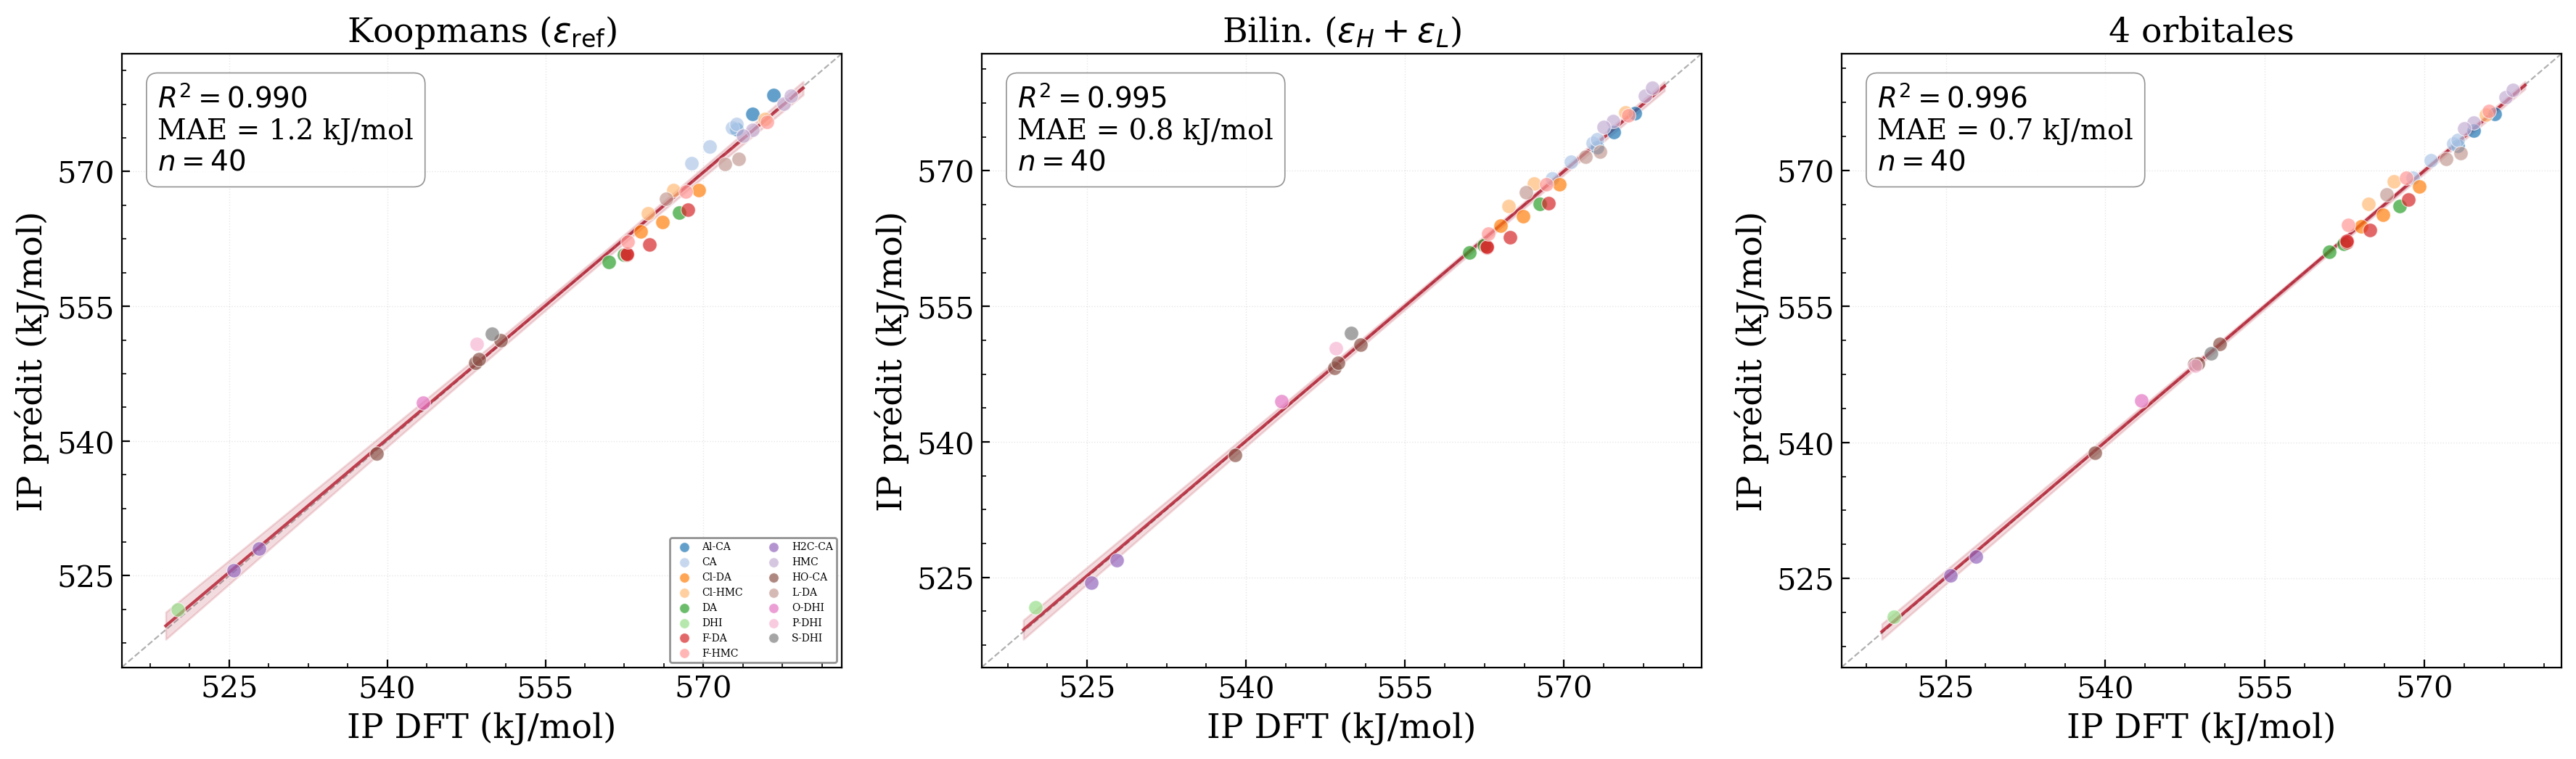
\includegraphics[width=\textwidth]{beyond_koopmans/IP_3models_parity.png}
\caption{Prédiction de l'IP par les trois modèles de régression orbitale (15 catéchols, 40 conformères). De gauche à droite : Koopmans calibré ($\varepsilon_H$), bilinéaire ($\varepsilon_H + \varepsilon_L$), et 4 orbitales ($\varepsilon_{H-1}, \varepsilon_H, \varepsilon_L, \varepsilon_{L+1}$). Chaque point est un conformère, couleur par molécule.}
\label{fig:ip_3models}
\end{figure}

\paragraph{Résultats pour l'EA.}
Pour l'affinité électronique (tableau~\ref{tab:multi_orb_ea}, figure~\ref{fig:ea_3models}), le constat est différent : ni l'ajout de $\varepsilon_H$ ni celui des 4 orbitales n'améliore la prédiction de Koopmans. Aucun des descripteurs supplémentaires n'est significatif (tous $p > 0.7$), et la CV se dégrade à chaque paramètre ajouté. Le modèle optimal pour l'EA reste l'approximation de Koopmans calibrée :
\begin{equation}
\mathrm{EA} = -0.994\,\varepsilon_L + 34.2 \quad (\text{kJ/mol},\ \varepsilon\ \text{en kJ/mol})
\label{eq:ea_koopmans}
\end{equation}
Le coefficient de $\varepsilon_L$, très proche de $-1$, confirme la validité de l'approximation de Koopmans pour l'EA sur cette série.

\begin{table}[H]
\centering
\caption{Prédiction de EA par régression sur les énergies orbitales TZ2P ($n = 40$, 15 catéchols sans DEA). Les énergies orbitales sont exprimées en kJ/mol.}
\label{tab:multi_orb_ea}
\begin{tabular}{lccccc}
\toprule
Modèle & $R^2_{\text{adj}}$ & MAE & RMSE & CV-MAE & $F$-test \\
       &                     & (kJ/mol) & (kJ/mol) & (kJ/mol) & vs Koopmans \\
\midrule
Koopmans ($\varepsilon_L$) & 0.9984 & 1.66 & 2.40 & 1.90 & --- \\
$\varepsilon_H + \varepsilon_L$ & 0.9984 & 1.65 & 2.40 & 2.00 & $p = 0.72$ (ns) \\
4 orbitales & 0.9983 & 1.65 & 2.40 & 2.19 & $p = 0.99$ (ns) \\
\bottomrule
\end{tabular}
\end{table}

\begin{figure}[H]
\centering
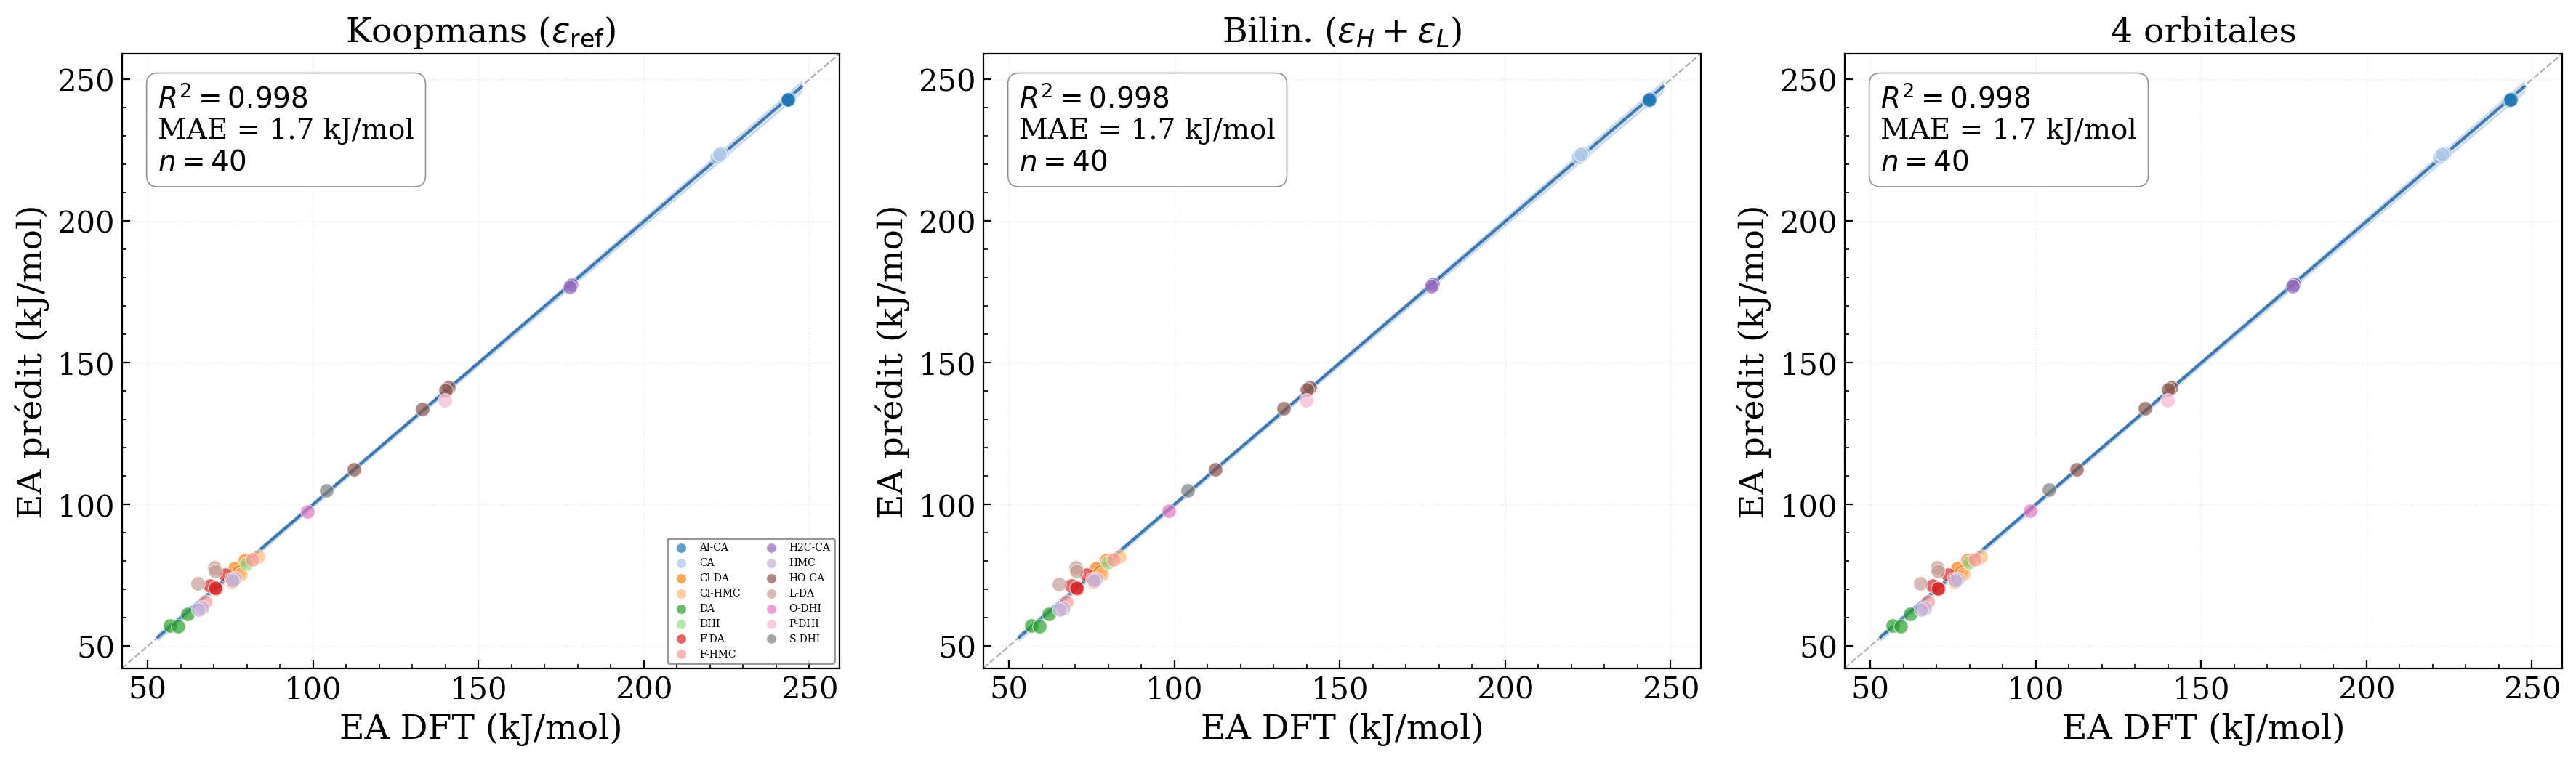
\includegraphics[width=\textwidth]{beyond_koopmans/EA_3models_parity.png}
\caption{Prédiction de EA par les trois modèles de régression orbitale (15 catéchols sans DEA, 40 conformères).}
\label{fig:ea_3models}
\end{figure}

\paragraph{Discussion.}
L'amélioration apportée par le second descripteur est marquée pour l'IP ($-26\%$ de MAE, $-21\%$ de CV-MAE) mais inexistante pour l'EA. L'origine de cette asymétrie est visible sur la figure~\ref{fig:resid_complement} : les résidus de Koopmans pour l'IP sont corrélés avec $\varepsilon_L$ ($r = +0.71$, $p = 3 \times 10^{-7}$), tandis que ceux de l'EA ne le sont avec aucun des descripteurs testés ($r = +0.06$ pour $\varepsilon_H$, $p = 0.72$). À HOMO égale, les molécules avec un gap HOMO--LUMO plus grand ont un IP systématiquement sous-estimé par Koopmans : le gap encode la dureté chimique, qui module l'amplitude de la relaxation orbitale post-ionisation.

\begin{figure}[H]
\centering
\begin{subfigure}[t]{0.48\textwidth}
\centering
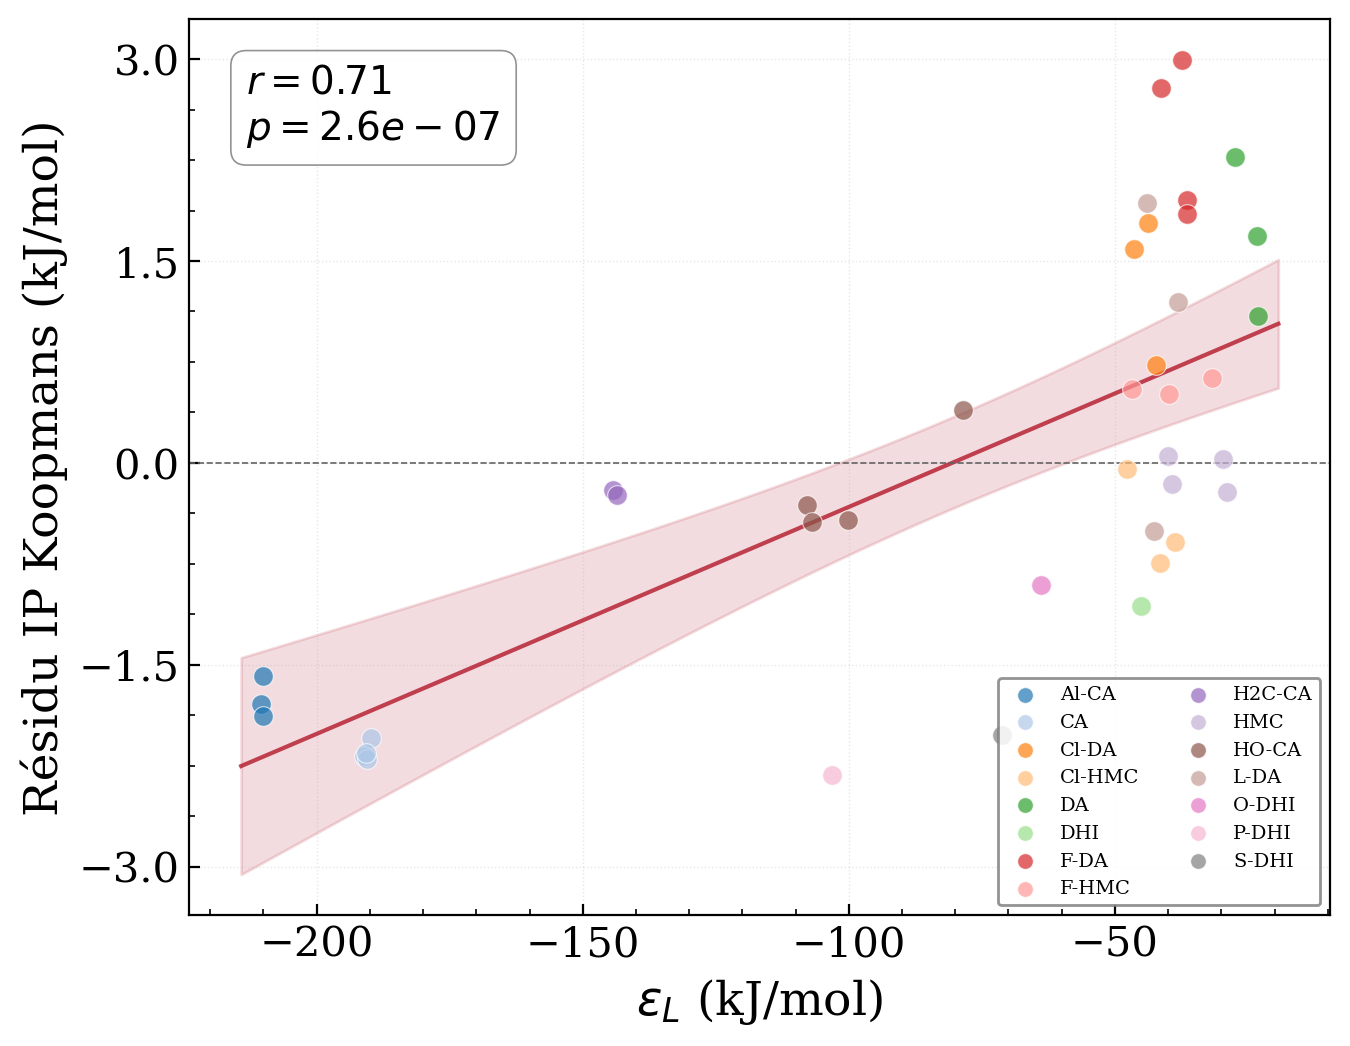
\includegraphics[width=\textwidth]{beyond_koopmans/residuals_ip_vs_lumo.png}
\caption{Résidu IP vs $\varepsilon_L$ ($r = 0.71$, $p = 3 \times 10^{-7}$).}
\label{fig:resid_ip}
\end{subfigure}
\hfill
\begin{subfigure}[t]{0.48\textwidth}
\centering
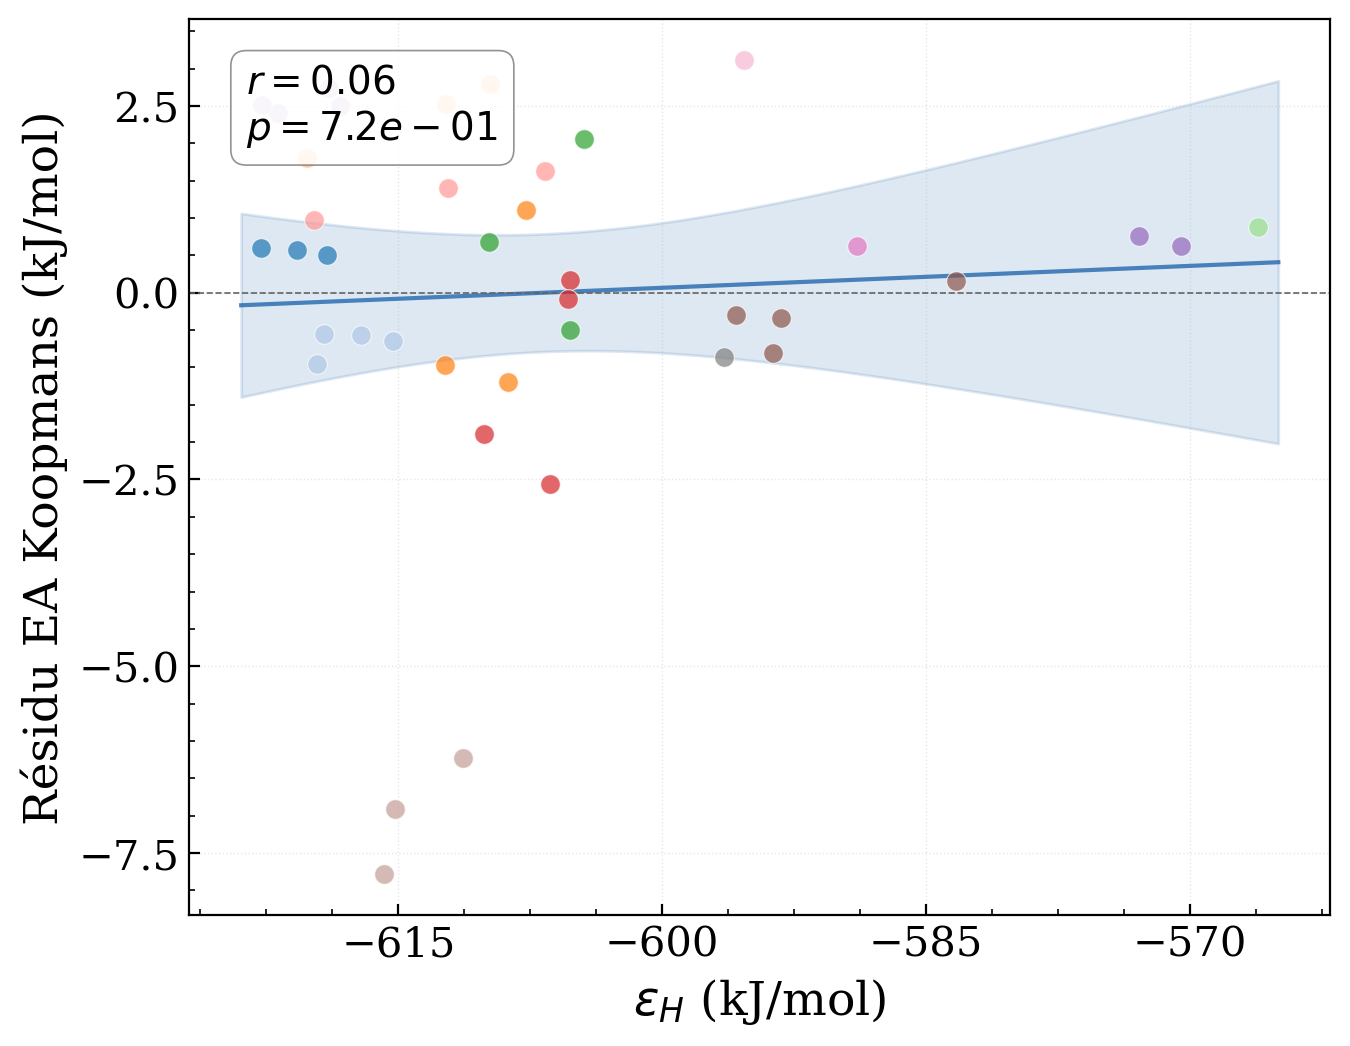
\includegraphics[width=\textwidth]{beyond_koopmans/residuals_ea_vs_homo.png}
\caption{Résidu EA vs $\varepsilon_H$ ($r = 0.06$, ns).}
\label{fig:resid_ea}
\end{subfigure}
\caption{Résidus de Koopmans en fonction de l'orbitale complémentaire (couleurs par molécule, $n = 40$). (a)~La corrélation significative montre que le gap HOMO--LUMO encode l'information manquante pour l'IP. (b)~Aucune corrélation pour l'EA.}
\label{fig:resid_complement}
\end{figure}

Cette asymétrie reflète la nature différente de la relaxation orbitale lors de l'ionisation versus la réduction. Lors du retrait d'un électron, les orbitales restantes se contractent, et l'amplitude de cette contraction dépend du gap --- une molécule plus dure (gap plus grand) relaxe moins, ce qui module l'écart à Koopmans. Lors de l'ajout d'un électron (réduction), la dilatation des orbitales occupées est plus uniforme et moins sensible au gap. Sur cette série chimiquement homogène de catéchols, l'EA est donc parfaitement prédite par $\varepsilon_L$ seule ($R^2 = 0.998$), tandis que l'IP bénéficie significativement de l'ajout de $\varepsilon_L$. Le modèle retenu est ainsi le bilinéaire $\varepsilon_H + \varepsilon_L$ pour l'IP et le Koopmans calibré pour l'EA.

\paragraph{Validation sur un jeu étendu.}
Pour vérifier la généralisabilité de ces conclusions, nous avons appliqué les trois modèles à un jeu de données élargi comprenant 70 molécules (catéchols, quinones, lignanes et dérivés halogénés) totalisant 167 conformères (tableau~\ref{tab:multi_orb_extended}). Les résultats confirment les tendances observées sur les 15 catéchols. Pour l'IP, le modèle bilinéaire apporte une amélioration significative ($p = 1.3 \times 10^{-4}$), réduisant la MAE de \SI{2.21}{kJ/mol} à \SI{1.98}{kJ/mol}. Le modèle à 4 orbitales n'améliore pas la CV-MAE, signe d'un léger surapprentissage sur ce jeu plus varié. Pour l'EA, l'approximation de Koopmans est remarquablement robuste ($R^2_{\text{adj}} = 0.999$, MAE $= \SI{2.14}{kJ/mol}$) et aucun descripteur supplémentaire n'apporte d'amélioration significative. On peut donc conclure que la correction bilinéaire par $\varepsilon_L$ est justifiée pour la prédiction de l'IP, tandis que l'EA est déjà optimalement prédite par $\varepsilon_L$ seule via l'approximation de Koopmans.

\begin{table}[H]
\centering
\caption{Prédiction de l'IP et de l'EA sur un jeu étendu de 70 molécules (167 conformères). Les énergies orbitales sont exprimées en kJ/mol.}
\label{tab:multi_orb_extended}
\footnotesize
\begin{tabular}{llccccc}
\toprule
 & Modèle & $R^2_{\text{adj}}$ & MAE & RMSE & CV-MAE & $F$-test \\
 &        &                     & (kJ/mol) & (kJ/mol) & (kJ/mol) & vs Koopmans \\
\midrule
\multirow{3}{*}{IP}
& Koopmans ($\varepsilon_H$) & 0.9914 & 2.21 & 3.84 & 2.31 & --- \\
& $\varepsilon_H + \varepsilon_L$ & 0.9921 & 1.98 & 3.67 & 2.09 & $p = 1.3 \times 10^{-4}$ \\
& 4 orbitales & 0.9927 & 2.04 & 3.51 & 2.27 & $p = 1.9 \times 10^{-6}$ \\
\midrule
\multirow{3}{*}{EA}
& Koopmans ($\varepsilon_L$) & 0.9990 & 2.14 & 3.74 & 2.19 & --- \\
& $\varepsilon_H + \varepsilon_L$ & 0.9990 & 2.11 & 3.73 & 2.18 & $p = 0.31$ (ns) \\
& 4 orbitales & 0.9990 & 2.11 & 3.73 & 2.21 & $p = 0.78$ (ns) \\
\bottomrule
\end{tabular}
\end{table}

\subsection{Corrélations de $E_{\text{relax}}$}

Contrairement à EA et IP, il n'existe pas de théorème général reliant $E_{\text{relax}}$ aux propriétés de l'état neutre. L'approche vibronique de référence pour prédire cette grandeur est le couplage vibronique linéaire (LVC), que nous avons appliqué systématiquement avant d'en analyser les limites.

\subsubsection{Prédiction par couplage vibronique linéaire}
\label{sec:lvc}

L'approche LVC estime l'énergie de relaxation par le développement quadratique de la PES ionique autour de la géométrie neutre $R_0$. Sous forme matricielle :
\begin{equation}
E_{\text{relax}} \approx -\tfrac{1}{2}\,\boldsymbol{g}^T \mathbf{H}^{-1} \boldsymbol{g}
\label{eq:lvc_matrix}
\end{equation}
où $\boldsymbol{g} = \nabla V_{\text{ion}}(R_0)$ est le gradient de la PES ionique à la géométrie neutre et $\mathbf{H}$ est un Hessien. En décomposant sur les modes normaux $\mathbf{N}_i$ (vecteurs propres de $\mathbf{H}$, normalisés à 1 en espace cartésien) :
\begin{equation}
E_{\text{relax}}^{\text{LVC}} = -\sum_i \frac{F_i^2}{2k_i}, \quad F_i = \boldsymbol{g} \cdot \mathbf{N}_i
\label{eq:lvc}
\end{equation}
où $k_i$ est la constante de force (valeur propre du Hessien projeté sur le mode $i$, en Hartree/Bohr$^2$). La question cruciale est : \emph{quel Hessien utiliser ?} Nous distinguons deux variantes selon le choix du Hessien.

\paragraph{LVC1 : Hessien neutre.}
L'approche classique utilise le Hessien de l'état neutre ($\mathbf{H}_{\text{neutre}}$), calculé lors de l'optimisation géométrique. Elle suppose implicitement que la courbure de la PES ionique est identique à celle de la PES neutre, c'est-à-dire que les modes normaux et constantes de force ne changent pas lors du transfert d'électron.

\paragraph{LVC2 : Hessien ionique.}
La seconde variante remplace $\mathbf{H}_{\text{neutre}}$ par le Hessien ionique $\mathbf{H}_{\text{ion}}(R_0)$, évalué à la géométrie neutre lors du calcul single-point ionique (avec l'option \texttt{NormalModes}) :
\begin{equation}
E_{\text{relax}}^{\text{LVC2}} = -\sum_j \frac{F'^{\,2}_j}{2k'_j} = -\tfrac{1}{2}\,\boldsymbol{g}^T \mathbf{H}_{\text{ion}}^{-1} \boldsymbol{g}, \quad F'_j = \boldsymbol{g} \cdot \mathbf{N}'_j
\label{eq:lvc2}
\end{equation}
où $\mathbf{N}'_j$ et $k'_j$ sont les modes normaux et constantes de force du Hessien ionique. Cette formulation est exacte au second ordre du développement de Taylor de $V_{\text{ion}}$ autour de $R_0$ : gradient et courbure sont tous deux évalués sur la \emph{même} PES ionique, assurant la cohérence du développement. Le calcul ne requiert qu'un single-point ionique avec NormalModes activé --- les gradients et le Hessien sont extraits du même fichier RKF (le Hessien numérique est calculé par différences finies, $\sim 6N$ SCF additionnels).

\paragraph{Filtre des modes basse fréquence.} Le Hessien ionique évalué à la géométrie neutre n'est pas stationnaire : il contient des modes propres avec fréquences imaginaires (modes mous instabilisés par le transfert d'électron, attendus selon la théorie LVC) et des modes positifs très basse fréquence ($< \SI{50}{cm^{-1}}$) qui sont des artefacts numériques de l'approximation harmonique. Pour ces derniers, le terme $F'^{\,2}_j / (2k'_j)$ avec $k'_j \propto \omega_j^2 \to 0$ diverge artificiellement : un seul mode à $\omega = \SI{20}{cm^{-1}}$ avec $|F'_j| \sim \SI{e-3}{Ha/Bohr}$ contribue à lui seul $\sim \SI{e5}{kJ/mol}$. La somme de l'équation~\ref{eq:lvc2} est donc restreinte aux modes positifs de fréquence $\omega_j \geq \SI{50}{cm^{-1}}$. Ce seuil élimine les artefacts sans amputer la physique pertinente : les modes physiques (torsions, rotations de groupes) commencent typiquement vers \SI{50}{}--\SI{100}{cm^{-1}}, et faire varier le seuil entre 50 et \SI{200}{cm^{-1}} ne change le R² que de moins de 1\,\%.

\paragraph{Résultats.}
La figure~\ref{fig:lvc_scatter} compare les deux variantes. Le LVC1 avec Hessien neutre (a, c) surestime systématiquement $E_{\text{relax}}$ d'un facteur 3 à 20 (MAE $\approx \SI{90}{kJ/mol}$ pour les deux processus). Le LVC2 avec Hessien ionique (b, d) donne des prédictions excellentes après calibration linéaire : MAE de \SI{1.3}{kJ/mol} pour l'oxydation ($R^2 = 0.74$) et \SI{1.7}{kJ/mol} pour la réduction ($R^2 = 0.84$), soit une amélioration d'un facteur~50 à~70.

\begin{figure}[H]
\centering
\begin{subfigure}[t]{0.42\textwidth}
\centering
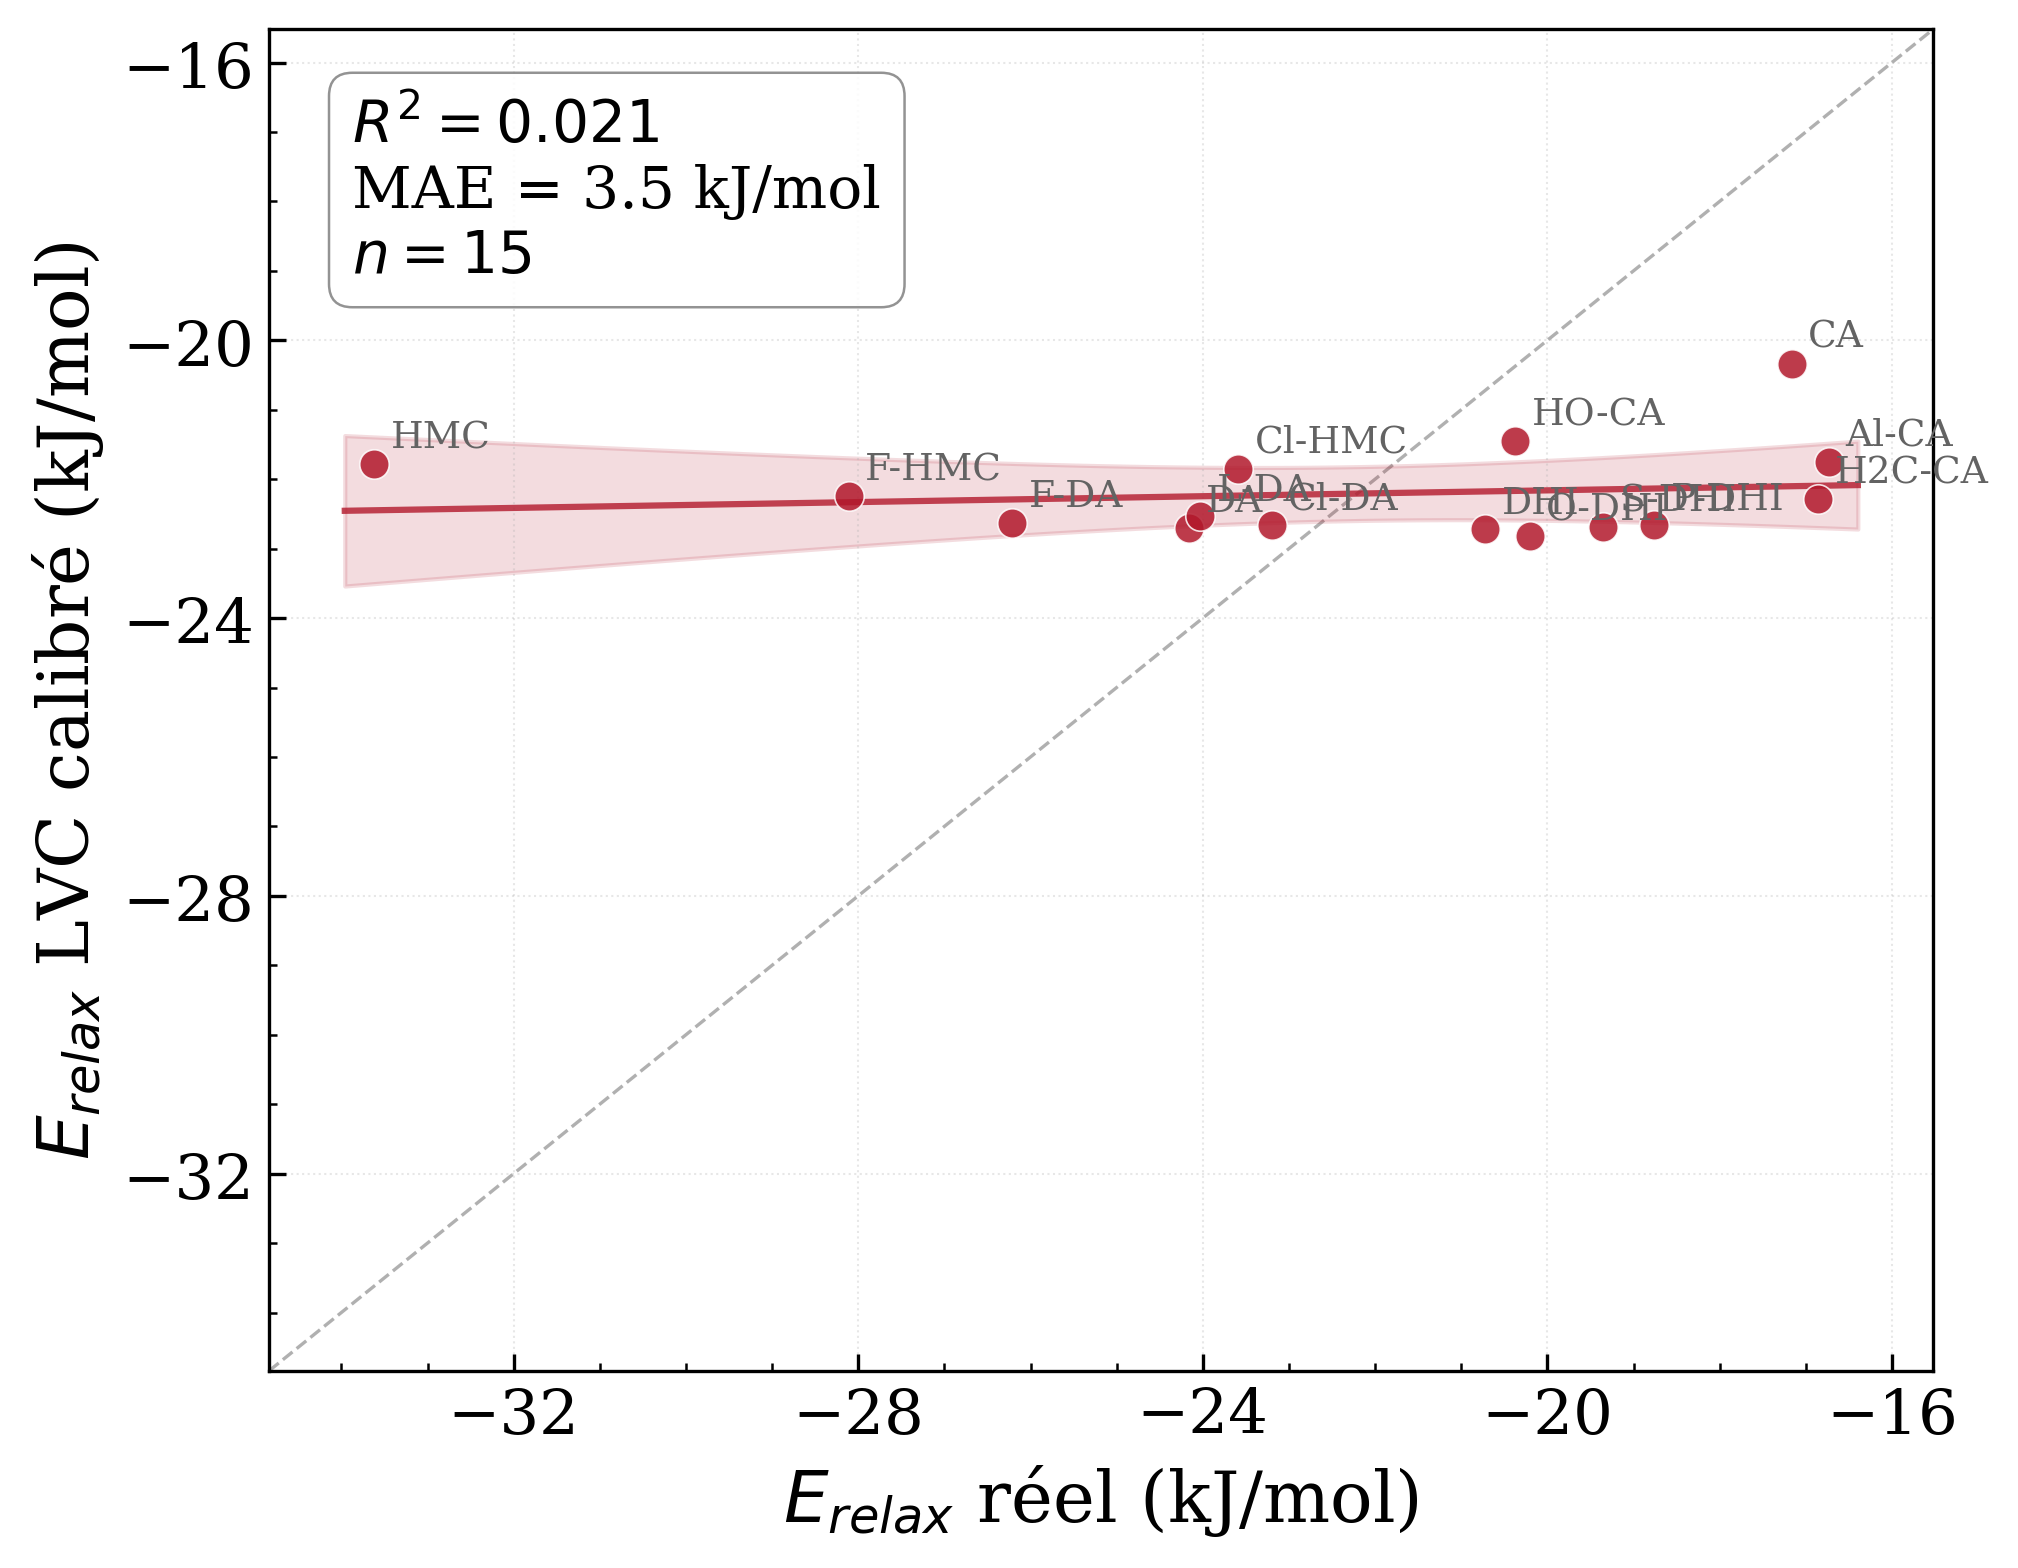
\includegraphics[width=\textwidth]{lvc_vs_real_oxidation.png}
\caption{Oxydation --- LVC1 ($R^2 = 0.02$, MAE $= \SI{90}{kJ/mol}$).}
\label{fig:lvc1_ox}
\end{subfigure}
\hfill
\begin{subfigure}[t]{0.42\textwidth}
\centering
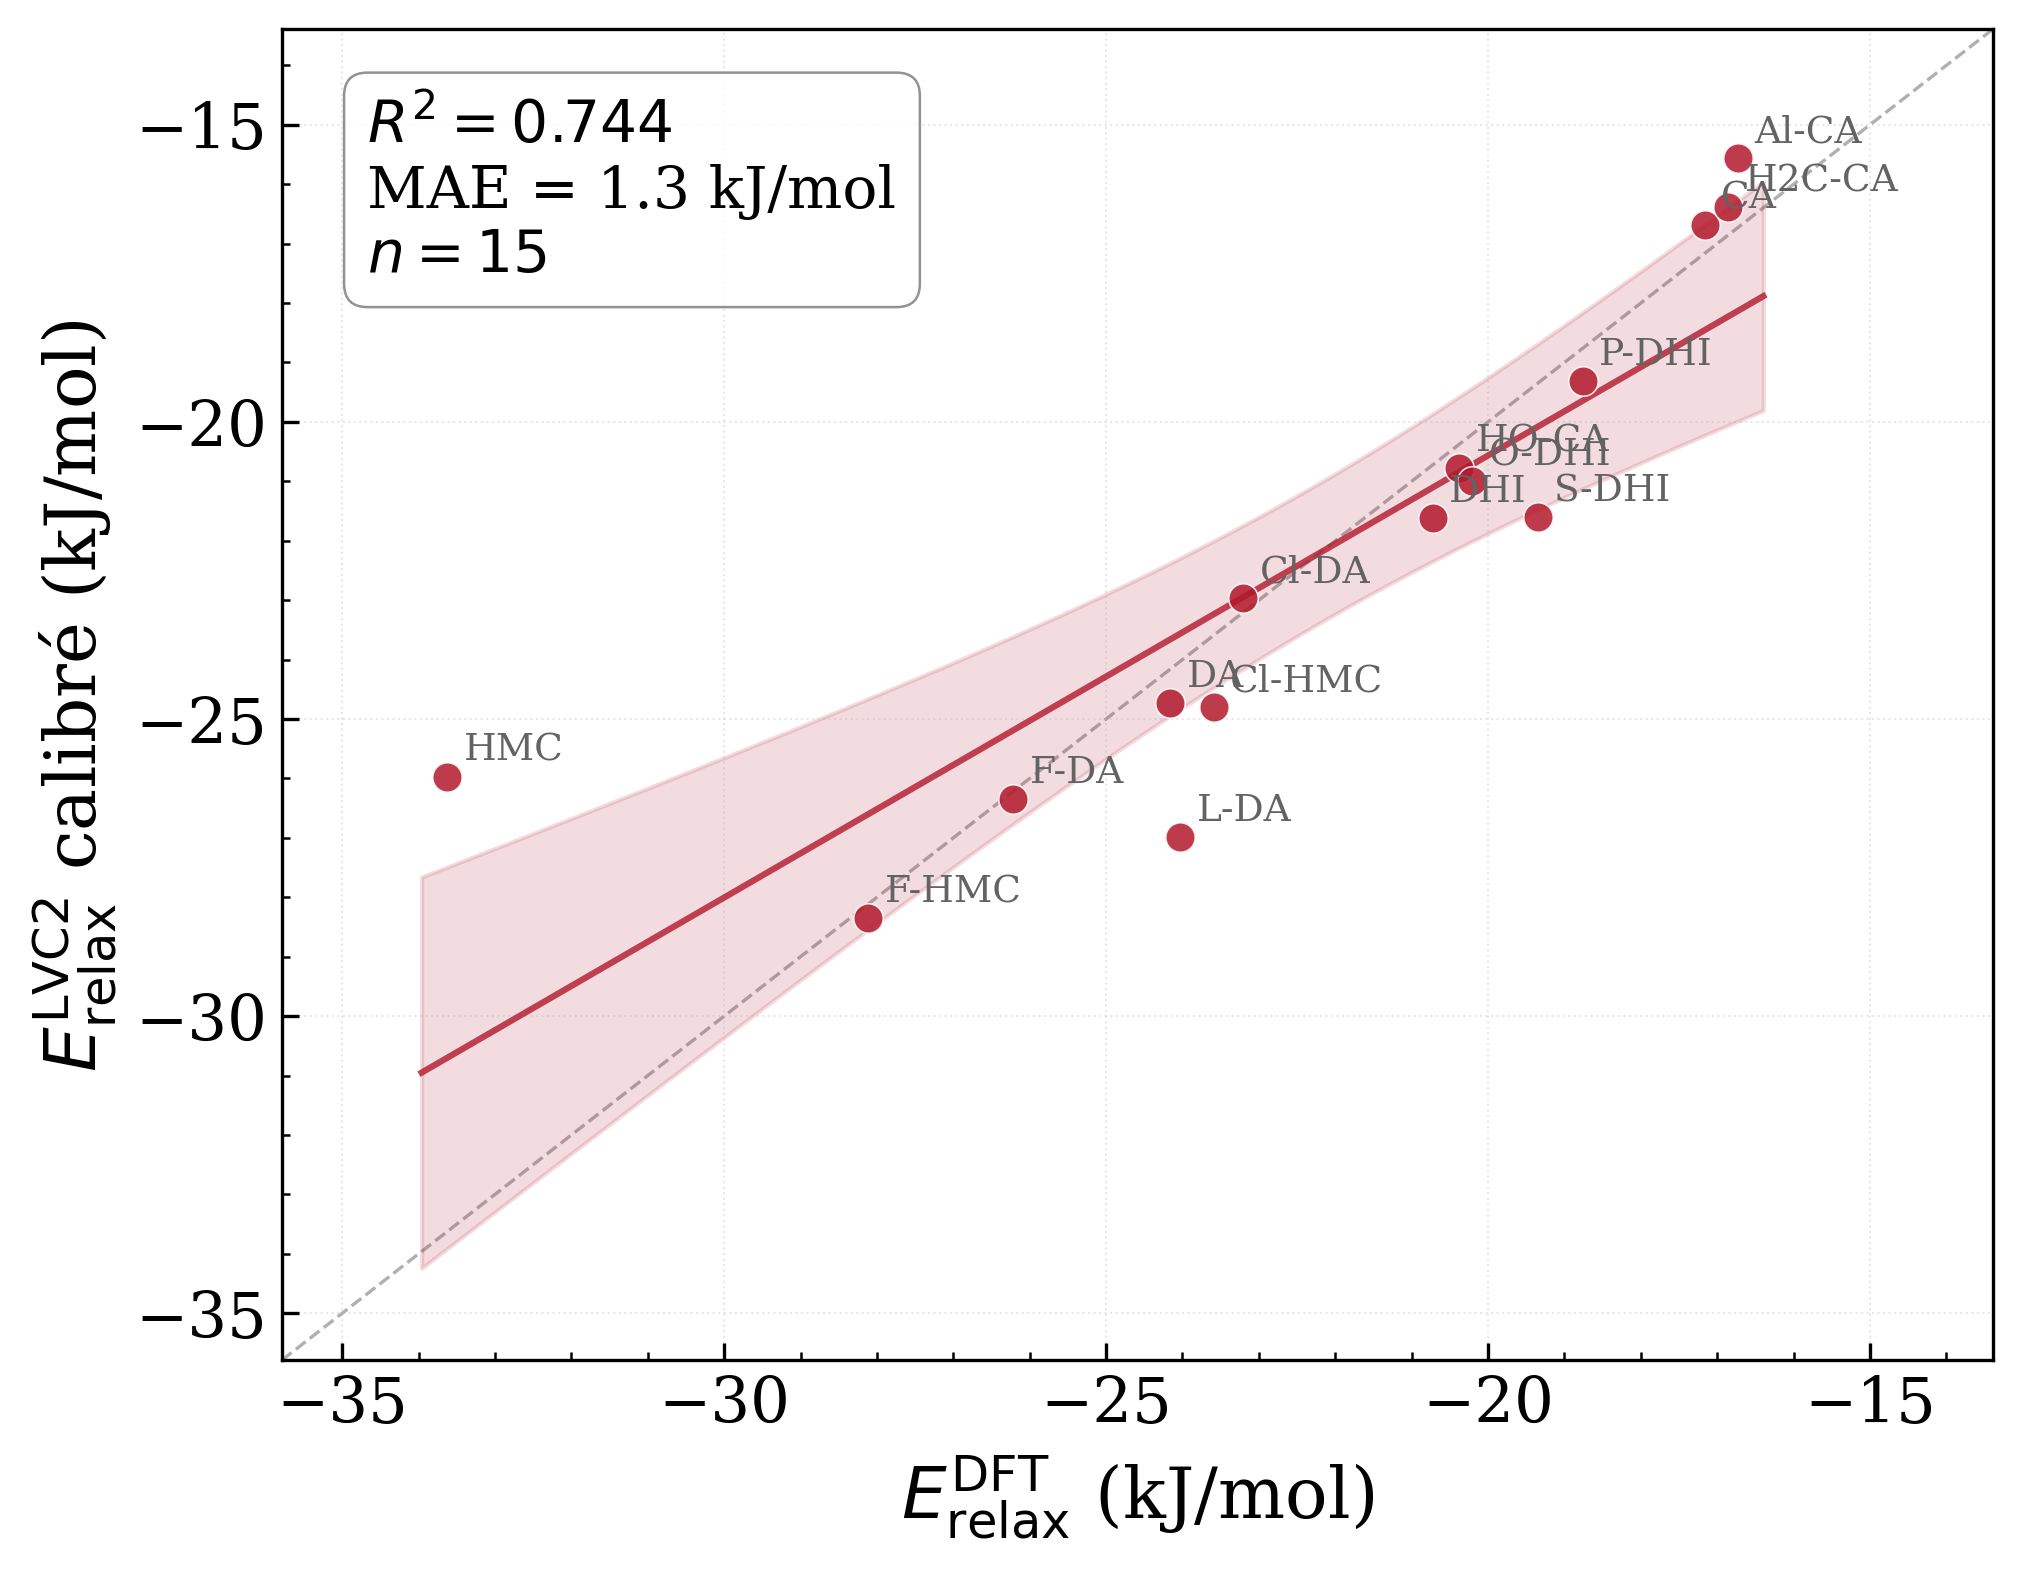
\includegraphics[width=\textwidth]{lvc2_brut_oxidation.png}
\caption{Oxydation --- LVC2 calibré ($R^2 = 0.74$, MAE $= \SI{1.3}{kJ/mol}$).}
\label{fig:lvc2_ox}
\end{subfigure}

\vspace{4pt}
\begin{subfigure}[t]{0.42\textwidth}
\centering
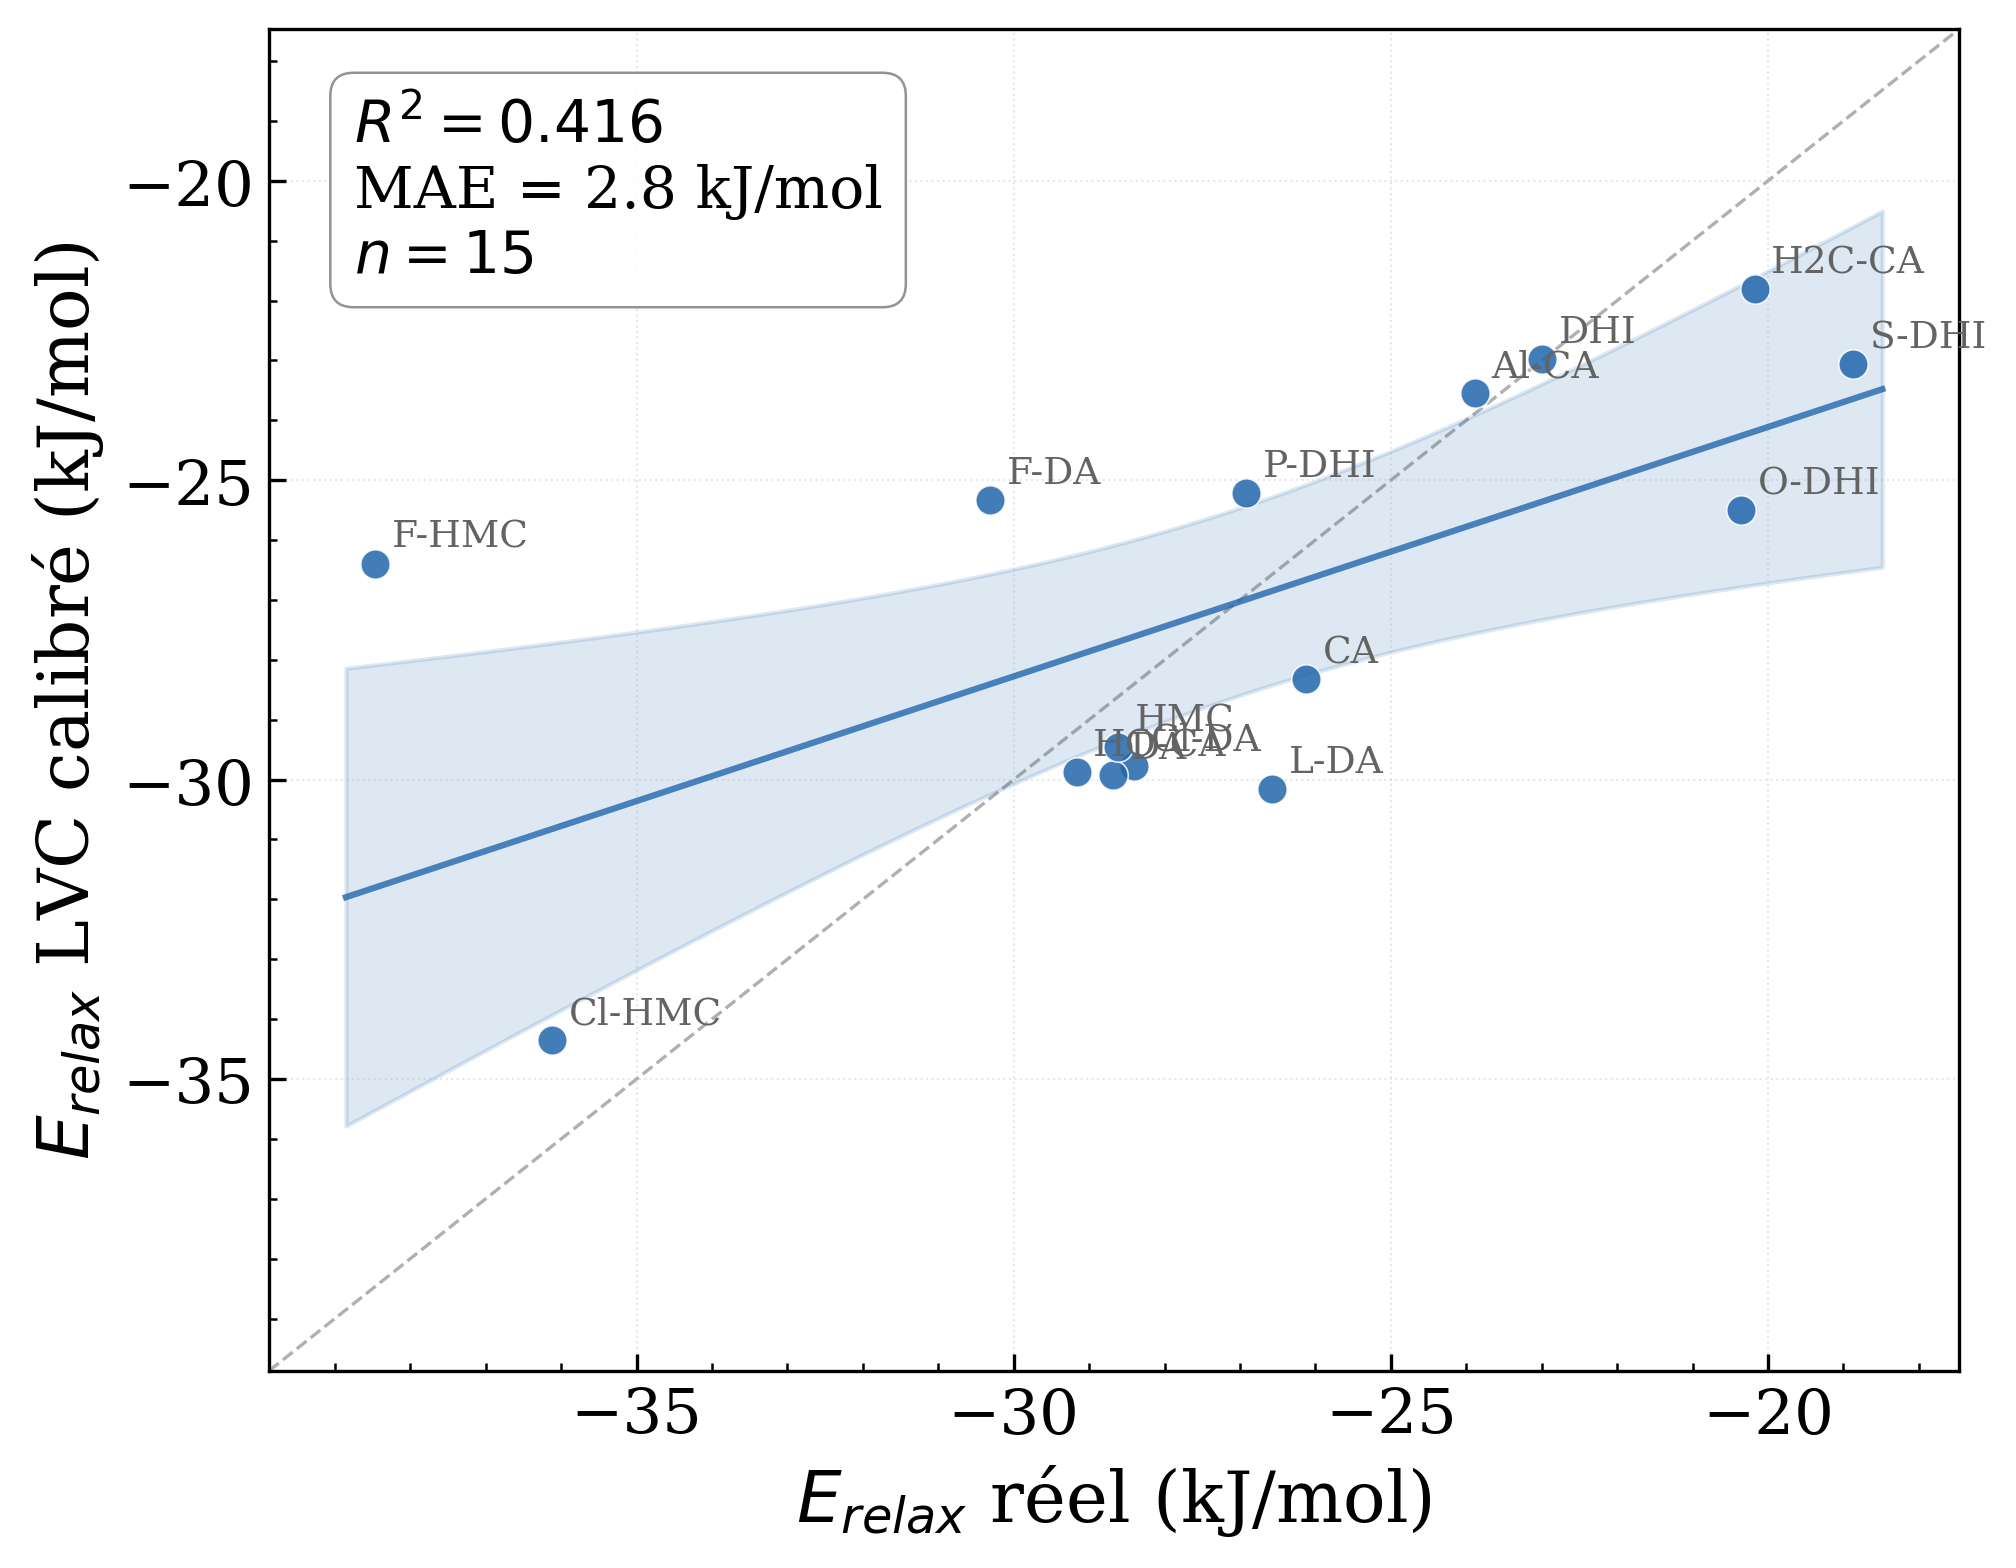
\includegraphics[width=\textwidth]{lvc_vs_real_reduction.png}
\caption{Réduction --- LVC1 ($R^2 = 0.42$, MAE $= \SI{90}{kJ/mol}$).}
\label{fig:lvc1_red}
\end{subfigure}
\hfill
\begin{subfigure}[t]{0.42\textwidth}
\centering
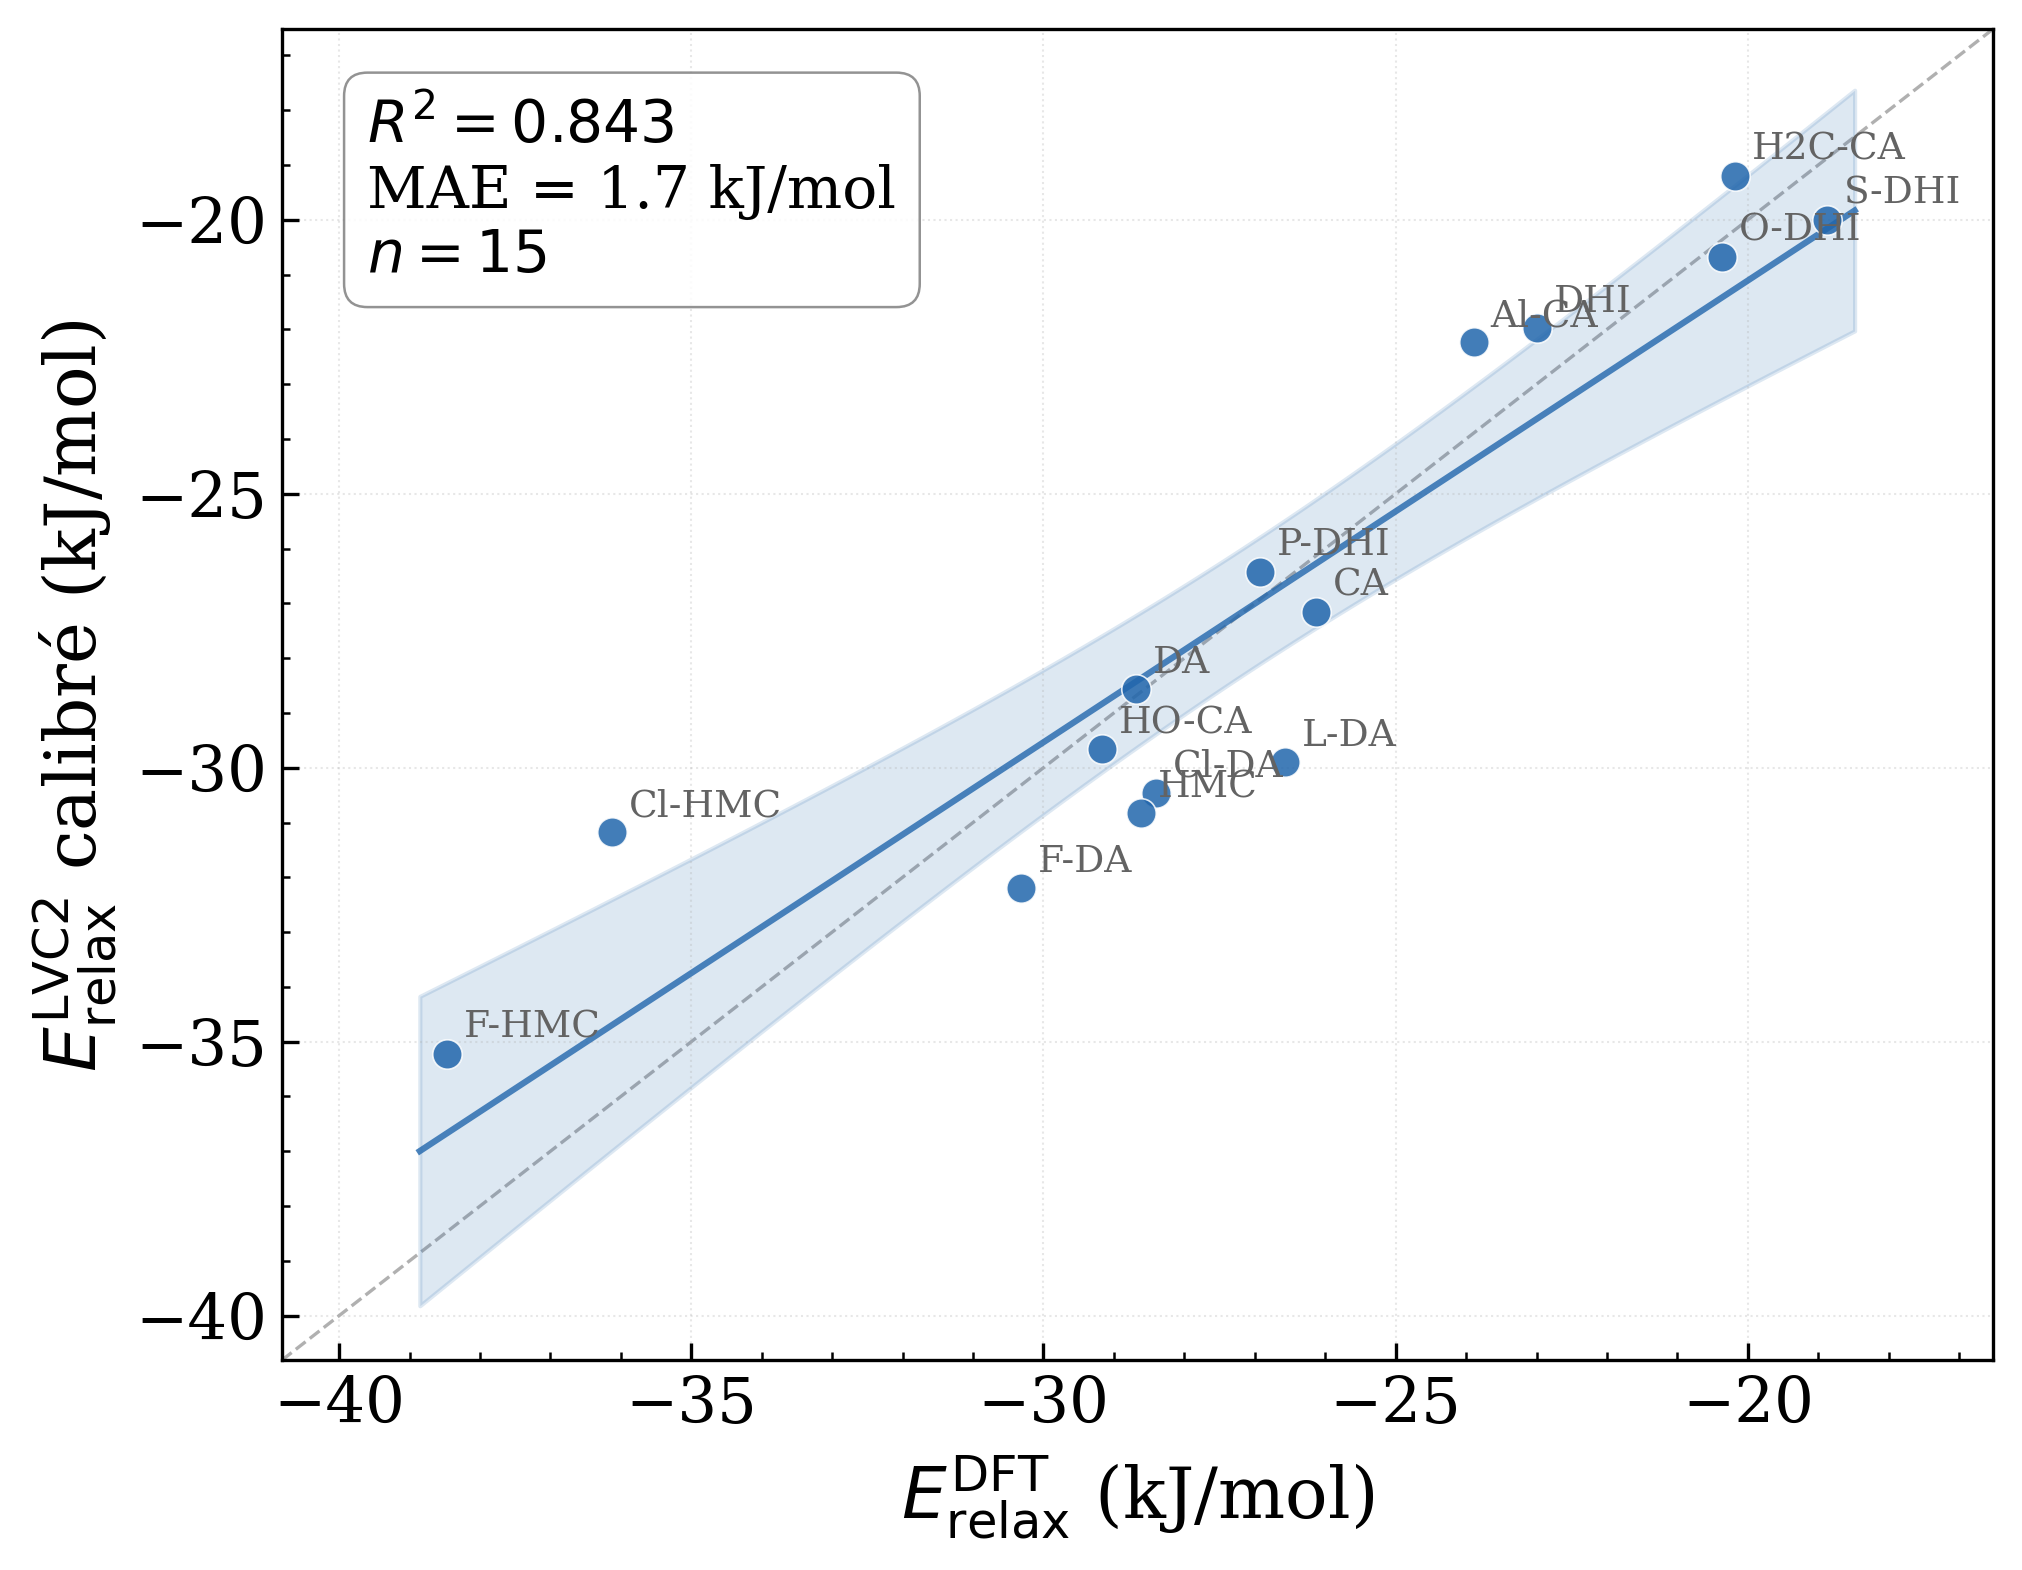
\includegraphics[width=\textwidth]{lvc2_brut_reduction.png}
\caption{Réduction --- LVC2 calibré ($R^2 = 0.84$, MAE $= \SI{1.7}{kJ/mol}$).}
\label{fig:lvc2_red}
\end{subfigure}
\caption{Prédiction de $E_{\text{relax}}$ par couplage vibronique linéaire. Gauche : LVC1 (Hessien neutre, calibré), droite : LVC2 (Hessien ionique, calibré). La ligne pointillée représente $y = x$ (accord parfait). $n = 15$ molécules.}
\label{fig:lvc_scatter}
\end{figure}

La figure~\ref{fig:bars} synthétise la comparaison molécule par molécule entre les valeurs LVC2 prédites et les valeurs DFT réelles. L'accord est remarquable pour les deux processus, les barres prédites se superposant quasi-parfaitement aux barres DFT.

\begin{figure}[H]
\centering
\begin{subfigure}[t]{0.48\textwidth}
\centering
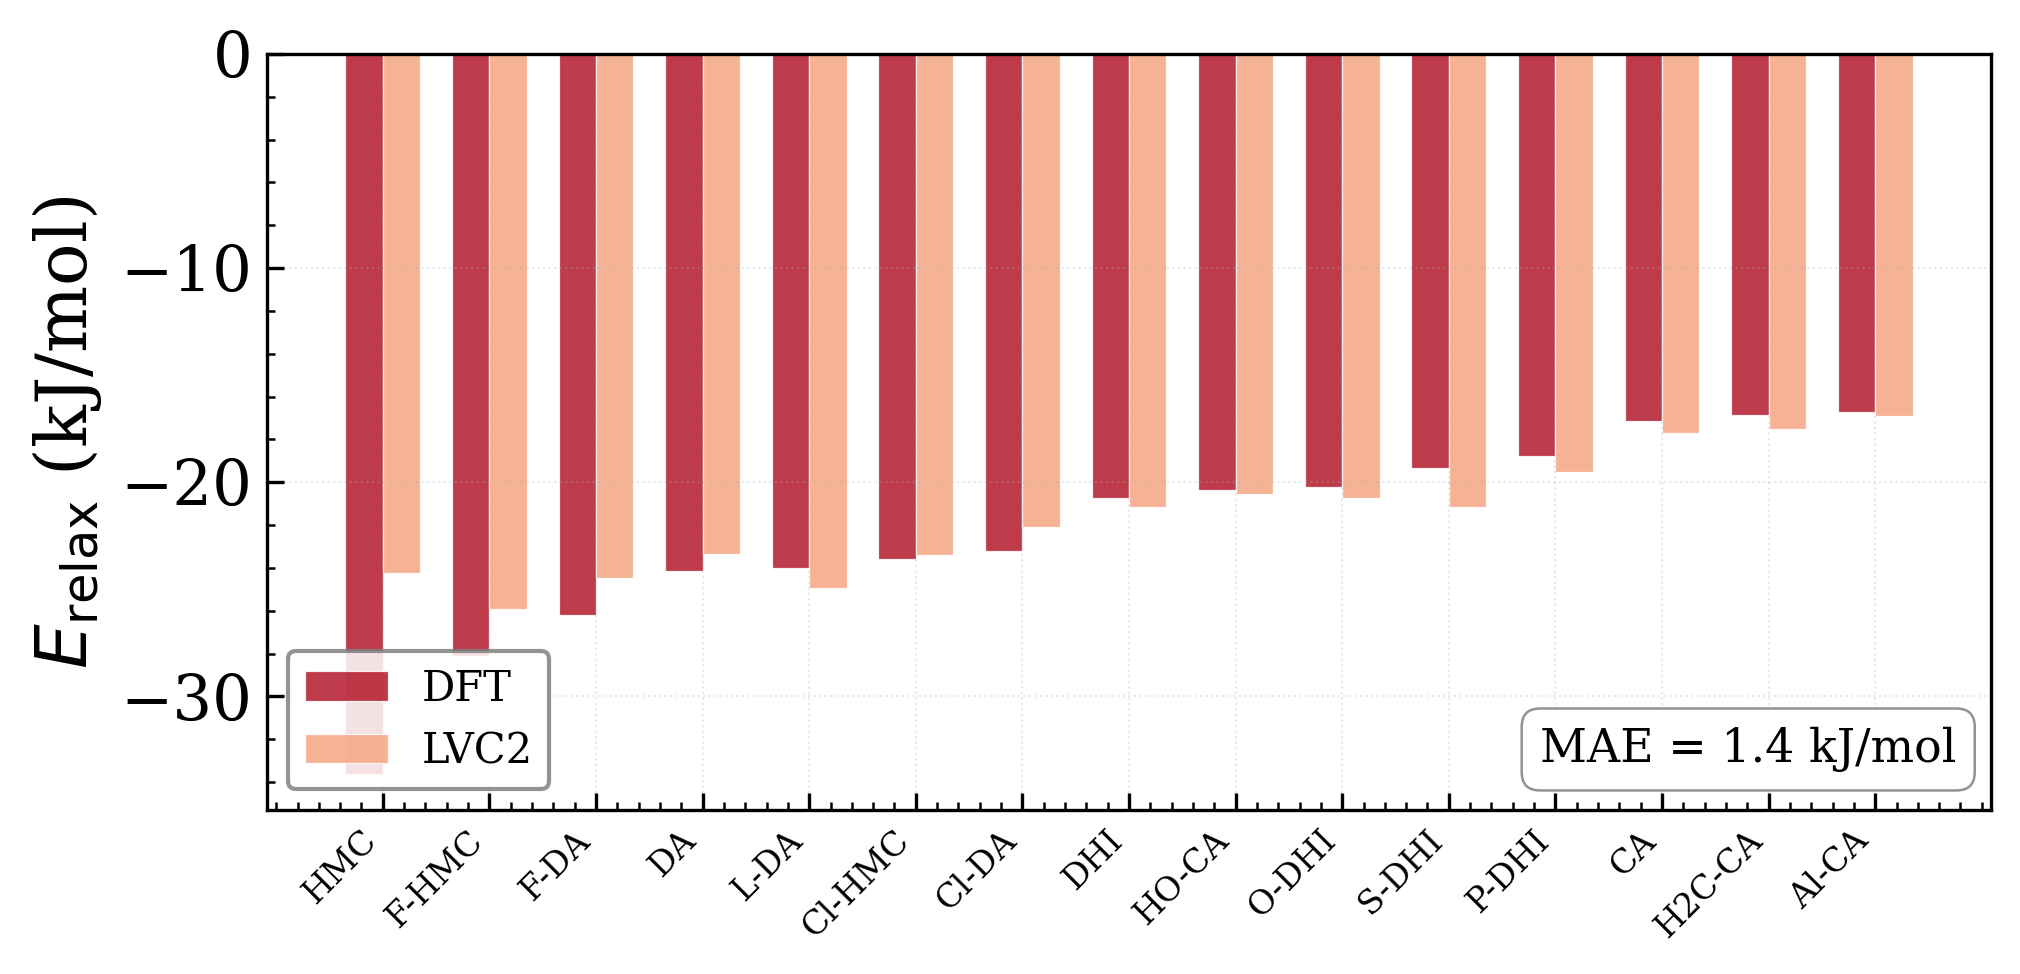
\includegraphics[width=\textwidth]{lvc_vs_real_bars_ox.png}
\caption{Oxydation (MAE $= \SI{1.4}{kJ/mol}$).}
\label{fig:bars_ox}
\end{subfigure}
\hfill
\begin{subfigure}[t]{0.48\textwidth}
\centering
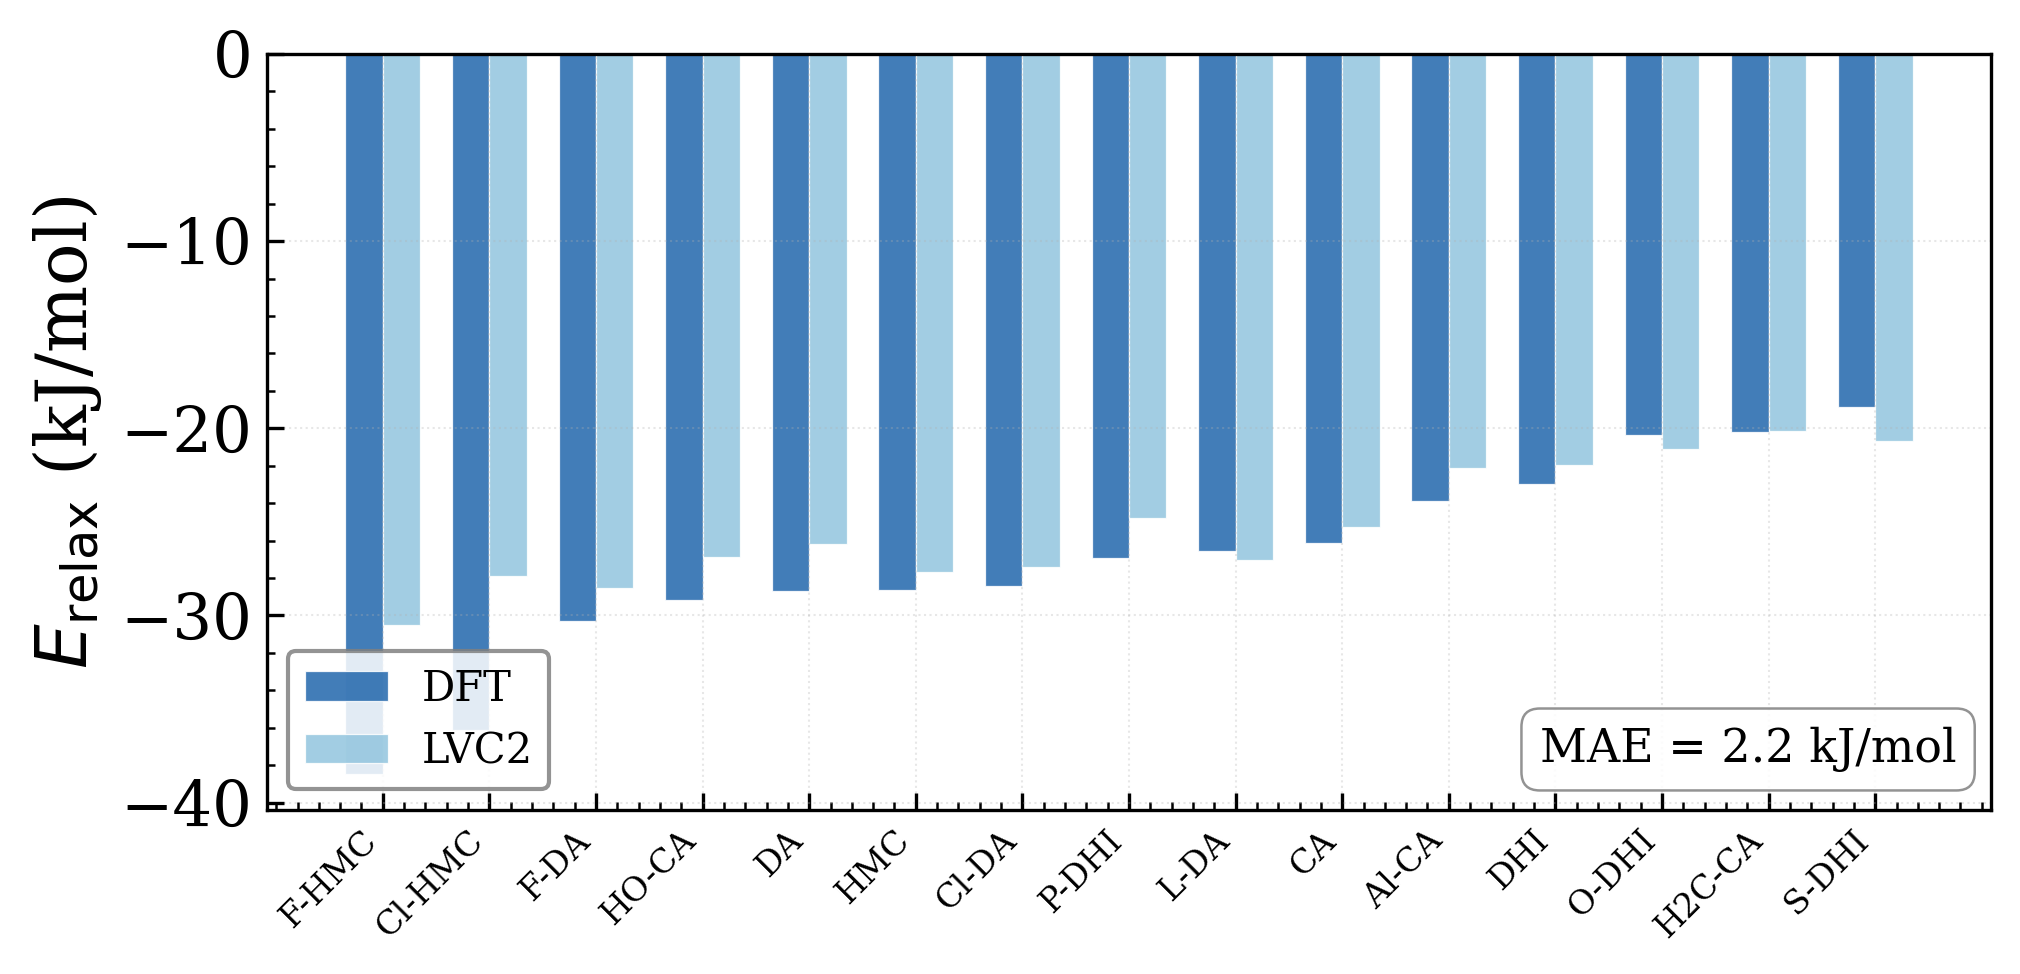
\includegraphics[width=\textwidth]{lvc_vs_real_bars_red.png}
\caption{Réduction (MAE $= \SI{2.2}{kJ/mol}$).}
\label{fig:bars_red}
\end{subfigure}
\caption{Comparaison LVC2 (prédit) vs DFT (réel) de $E_{\text{relax}}$ pour chaque molécule. Les barres sont triées par $E_{\text{relax}}$ DFT croissant.}
\label{fig:bars}
\end{figure}

\paragraph{Discussion.}
L'échec du LVC1 est identifié par l'analyse mode par mode : les modes basse fréquence du neutre ($< \SI{200}{cm^{-1}}$) ont des constantes de force $k_i$ très faibles, et le terme $F_i^2/(2k_i)$ diverge. Par exemple, pour CA conf~1, le mode à $\SI{89}{cm^{-1}}$ ($k = 0{,}002$ Hartree/Bohr$^2$) contribue à lui seul $-107$ kJ/mol à l'estimation LVC1, alors que $E_{\text{relax}}^{\text{réel}} = -26$ kJ/mol. Ces modes mous du neutre (torsions, rotations de groupes latéraux) se raidissent significativement dans l'état ionique : le Hessien neutre n'est pas une bonne approximation du Hessien ionique dans cette gamme de fréquences.

Le succès du LVC2 confirme que le problème n'est pas dans le formalisme LVC lui-même, mais dans le choix du Hessien. Évaluer gradient et courbure sur la \emph{même} PES ionique assure la cohérence du développement de Taylor au second ordre. Les MAE obtenues (\SIrange{1.4}{2.2}{kJ/mol}) sont comparables à l'incertitude intrinsèque de la fonctionnelle PBE0 ($\SIrange{4}{8}{kJ/mol}$). Toutefois, un résidu systématique subsiste en réduction pour certaines molécules, ce qui motive la recherche de corrections.

\subsubsection{Correction par la composition de la LUMO}
\label{sec:lumo_correction}

\paragraph{Théorie.}
Le résidu $E_{\text{relax}} - E_{\text{relax}}^{\text{LVC2}}$ est systématiquement négatif pour certaines molécules (le LVC2 prédit une relaxation insuffisante). Une analyse systématique des descripteurs moléculaires accessibles depuis le calcul neutre révèle que la \emph{fraction de la LUMO localisée sur les atomes d'oxygène} ($f_{\text{O}}^{\text{LUMO}}$, obtenue par analyse des populations SFO) est le meilleur prédicteur de ce résidu. Ce descripteur capture le caractère antiliant O--H de la LUMO : lorsque $f_{\text{O}}^{\text{LUMO}}$ est élevé, la réduction transfère un électron dans une orbitale qui affaiblit les liaisons O--H, entraînant un réarrangement géométrique important que l'approximation harmonique du LVC2 ne capte pas entièrement.

Le modèle de correction proposé est :
\begin{equation}
E_{\text{relax}}^{\text{corr}} = E_{\text{relax}}^{\text{LVC2}} \times \left(1 + \left(f_{\text{O}}^{\text{LUMO}}\right)^2\right)
\label{eq:lvc2_corr}
\end{equation}
Ce modèle ne comporte \emph{aucun paramètre libre} : le facteur $(1 + (f_{\text{O}}^{\text{LUMO}})^2)$ amplifie la relaxation LVC2 proportionnellement au caractère oxygène de la LUMO. Il n'y a donc aucun risque de surparamétrisation.

\paragraph{Résultats.}
La figure~\ref{fig:residual_fO} montre la corrélation entre le résidu LVC2 et $f_{\text{O}}^{\text{LUMO}}$ pour les deux processus. En réduction ($r = -0.68$, $p = 0.005$), les molécules à forte localisation de la LUMO sur les oxygènes (F-HMC : $f_{\text{O}} = 0.51$, Cl-HMC : $f_{\text{O}} = 0.36$) présentent les résidus les plus négatifs. En oxydation, la tendance est plus faible ($r = -0.49$, $p = 0.061$), cohérent avec un résidu déjà petit.

\begin{figure}[H]
\centering
\begin{subfigure}[t]{0.42\textwidth}
\centering
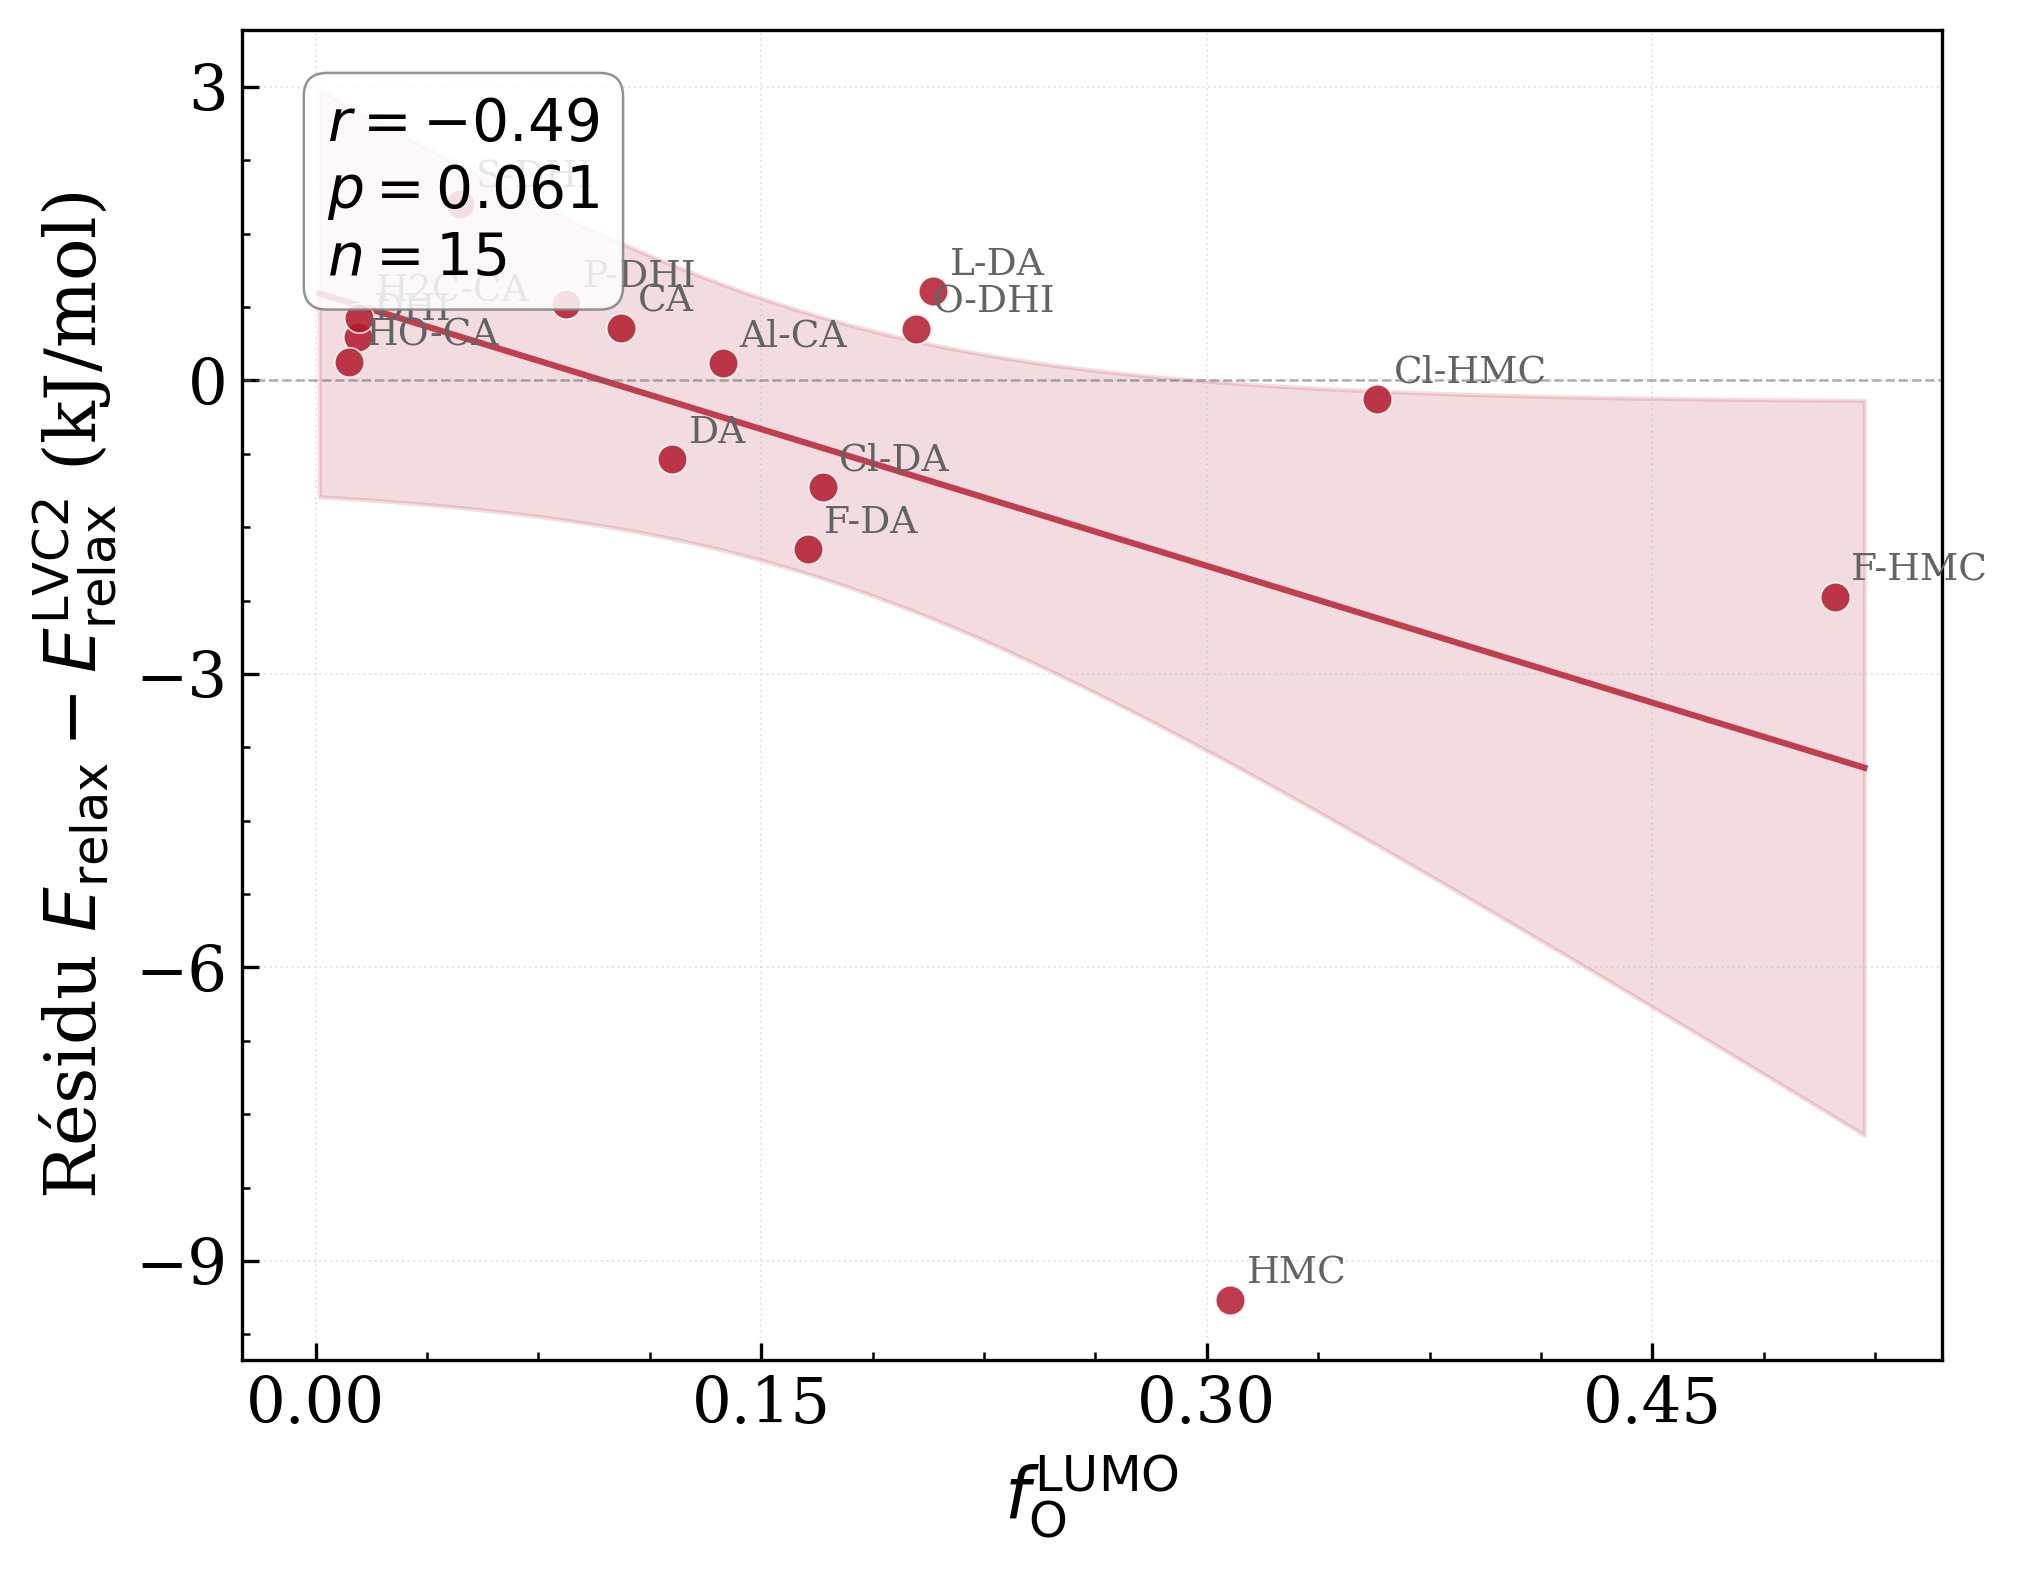
\includegraphics[width=\textwidth]{residual_lvc2_vs_fO_ox.png}
\caption{Oxydation ($r = -0.49$, $p = 0.061$).}
\label{fig:resid_fO_ox}
\end{subfigure}
\hfill
\begin{subfigure}[t]{0.42\textwidth}
\centering
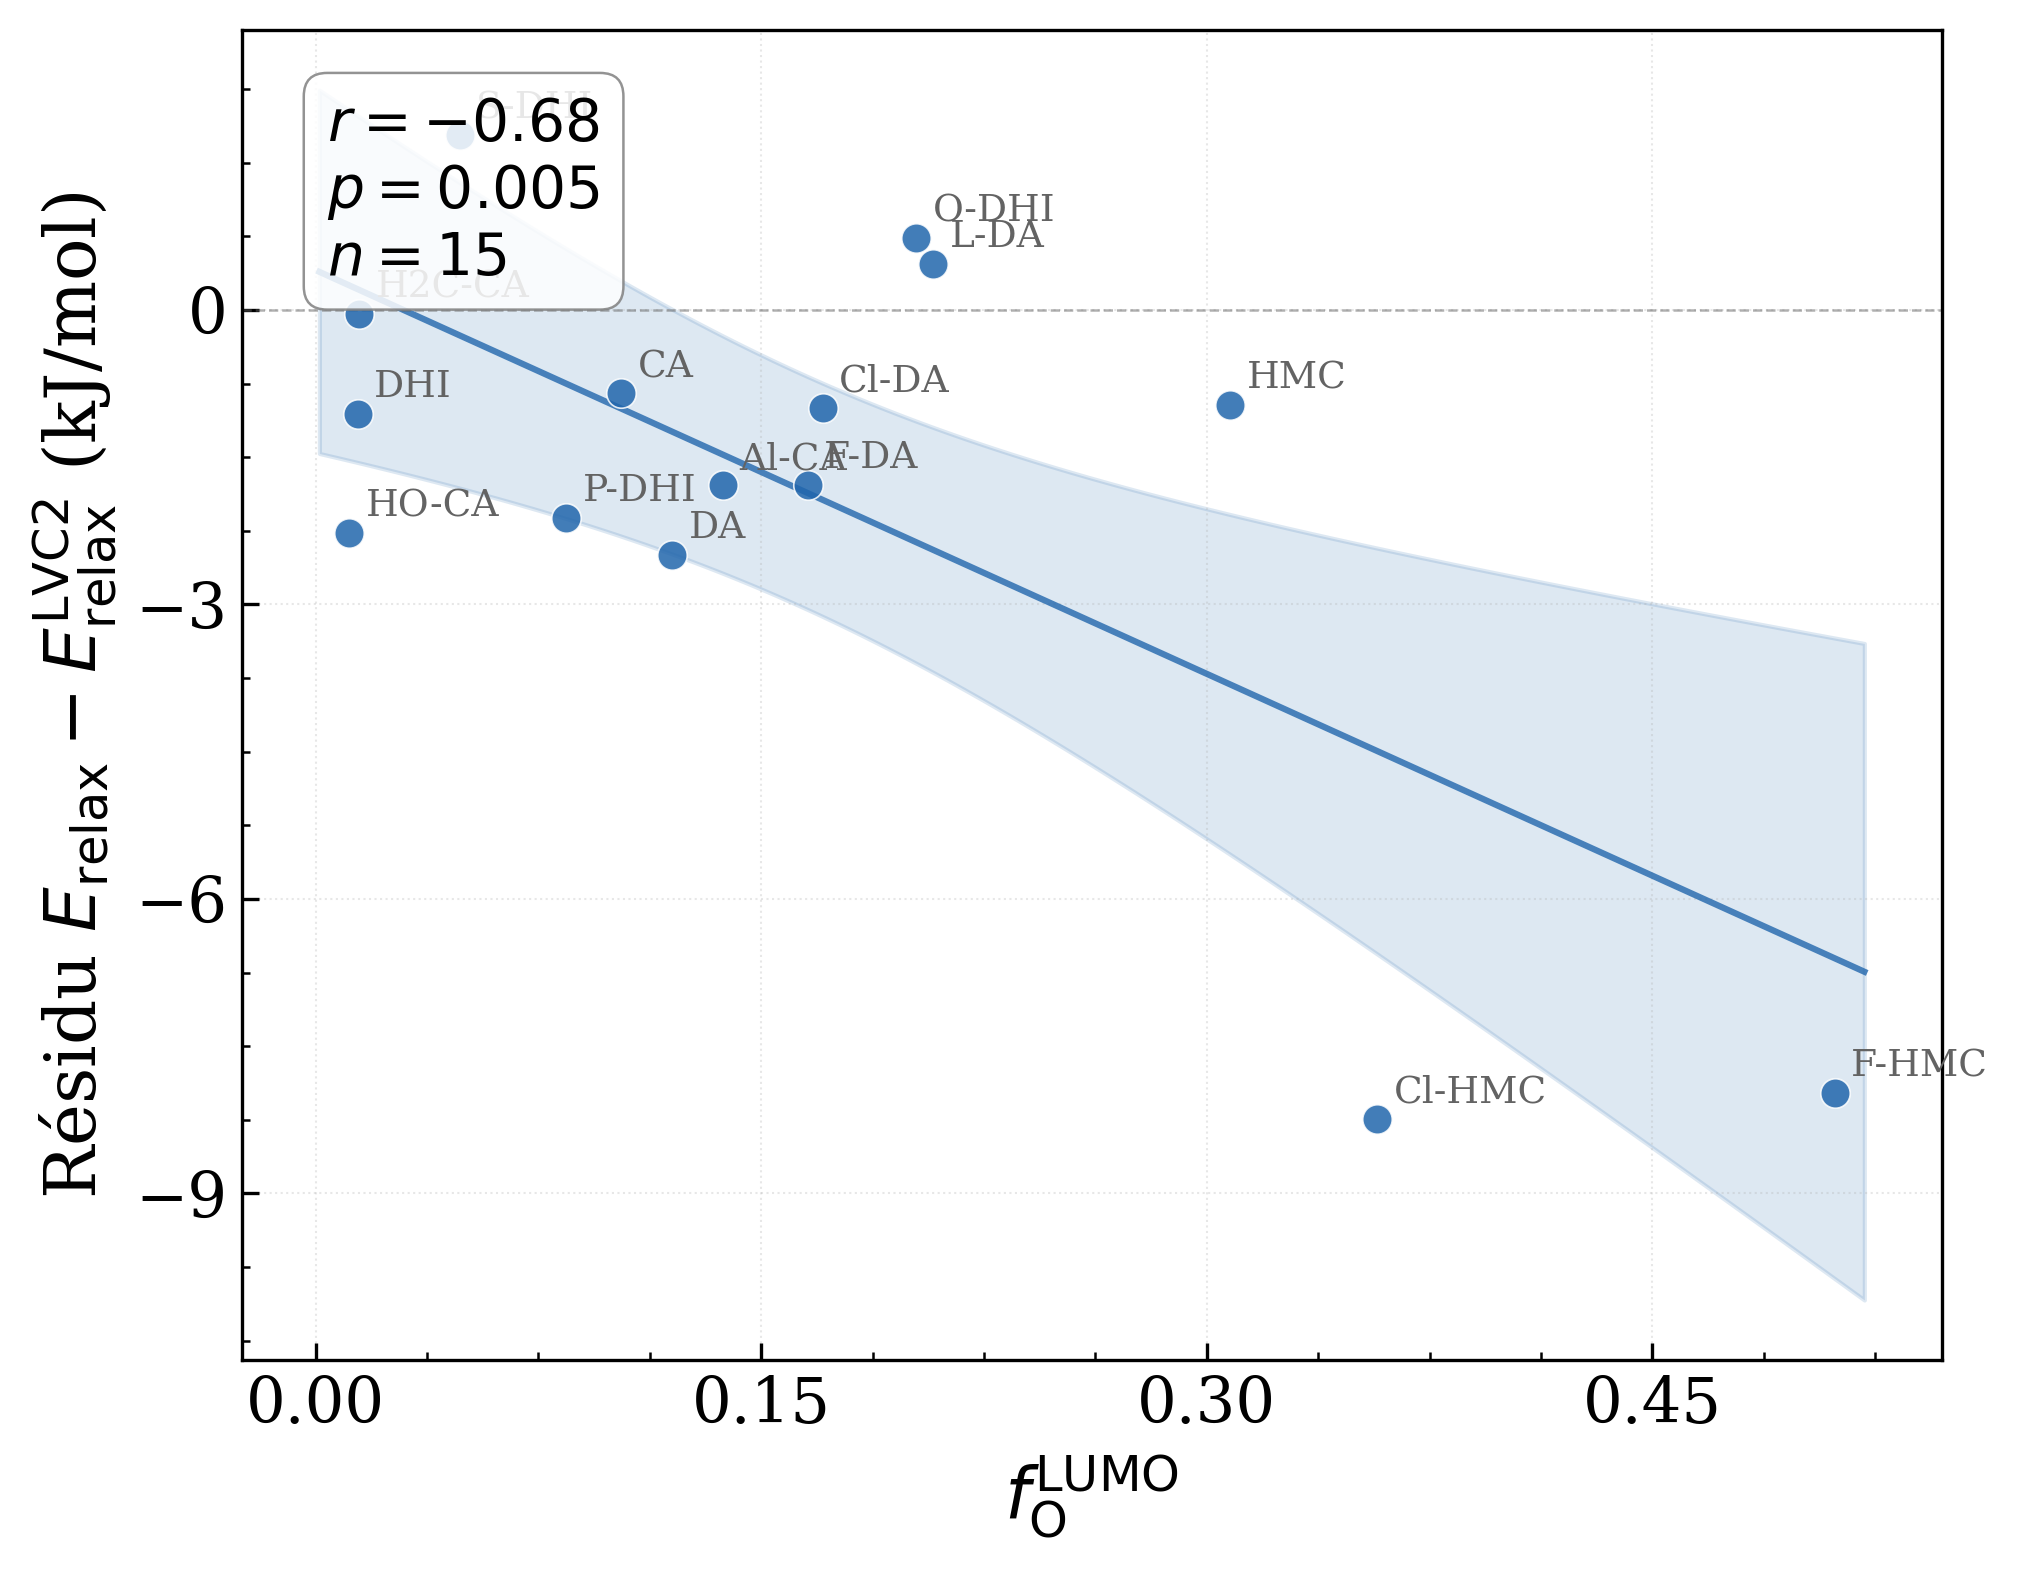
\includegraphics[width=\textwidth]{residual_lvc2_vs_fO_red.png}
\caption{Réduction ($r = -0.68$, $p = 0.005$).}
\label{fig:resid_fO_red}
\end{subfigure}
\caption{Résidu $E_{\text{relax}} - E_{\text{relax}}^{\text{LVC2}}$ en fonction de $f_{\text{O}}^{\text{LUMO}}$. La corrélation est significative en réduction (b) mais marginale en oxydation (a). $n = 15$ molécules.}
\label{fig:residual_fO}
\end{figure}

La figure~\ref{fig:lvc2_corrected} compare le LVC2 brut et le LVC2 corrigé pour les deux processus (parity plots calibrés). En réduction, la MAE calibrée passe de \SI{1.7}{kJ/mol} à \SI{1.4}{kJ/mol} ($R^2$ de $0.84$ à $0.89$). En oxydation, la correction n'apporte pas d'amélioration notable (MAE de $\SI{1.3}{kJ/mol}$ à $\SI{1.5}{kJ/mol}$), le résidu étant déjà quasi-nul.

\begin{figure}[H]
\centering
\begin{subfigure}[t]{0.42\textwidth}
\centering
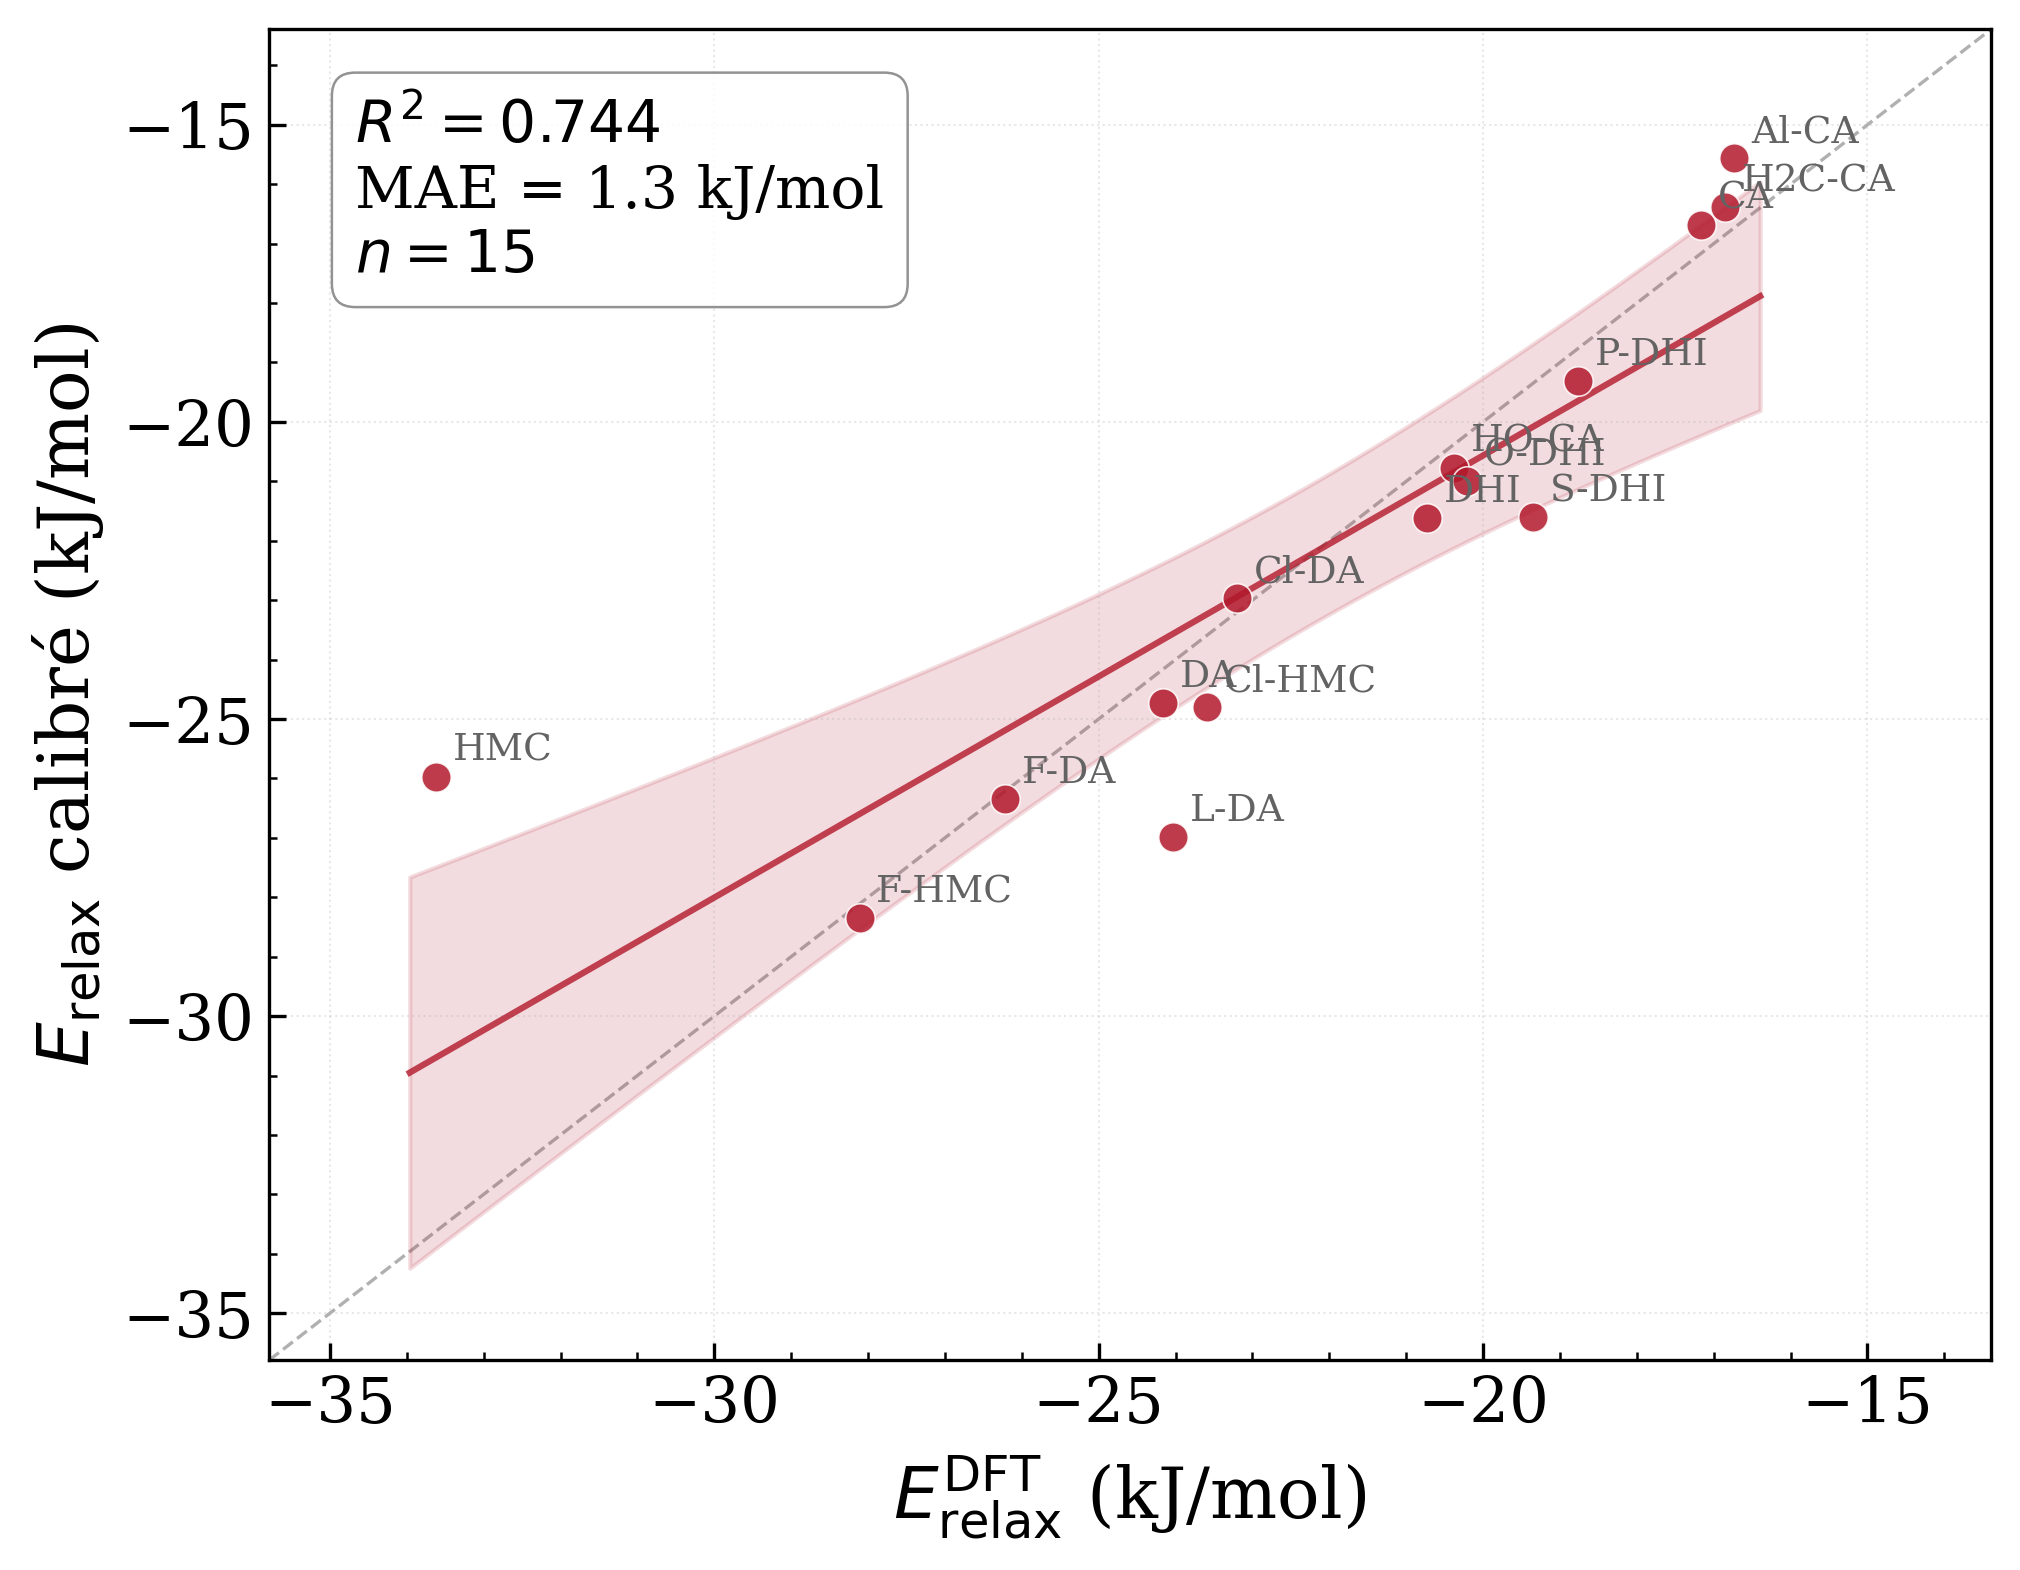
\includegraphics[width=\textwidth]{lvc2_brut_ox.png}
\caption{Oxydation --- LVC2 brut.}
\label{fig:lvc2_brut_ox}
\end{subfigure}
\hfill
\begin{subfigure}[t]{0.42\textwidth}
\centering
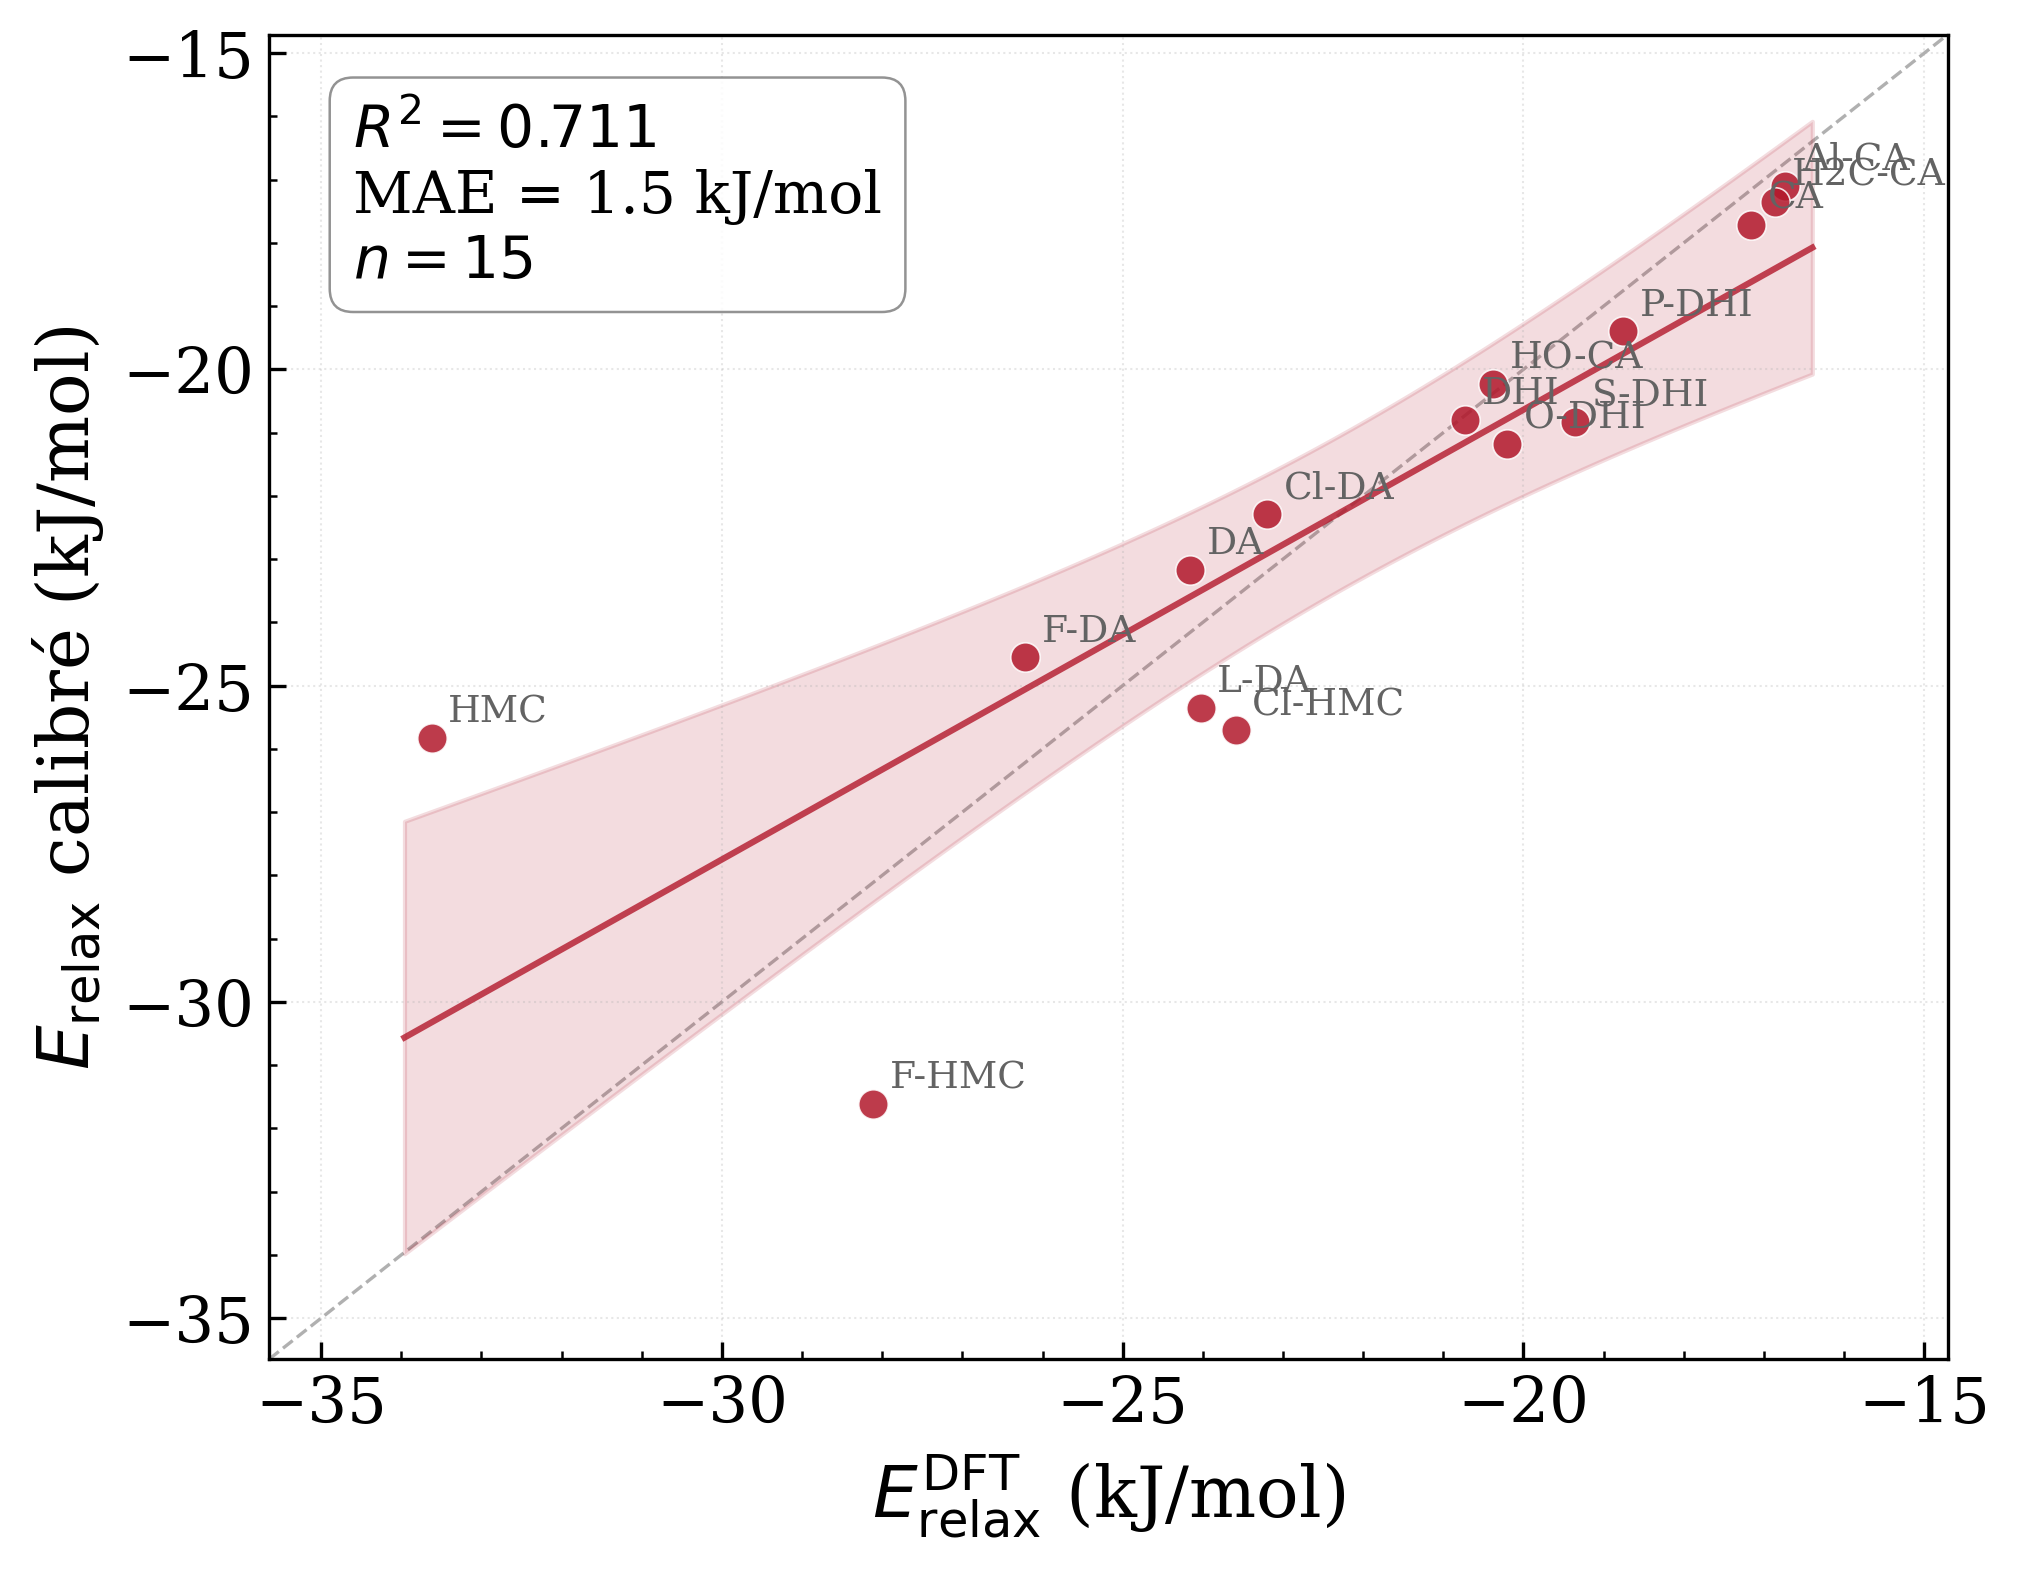
\includegraphics[width=\textwidth]{lvc2_corr_ox.png}
\caption{Oxydation --- LVC2 corrigé.}
\label{fig:lvc2_corr_ox}
\end{subfigure}

\vspace{4pt}
\begin{subfigure}[t]{0.42\textwidth}
\centering
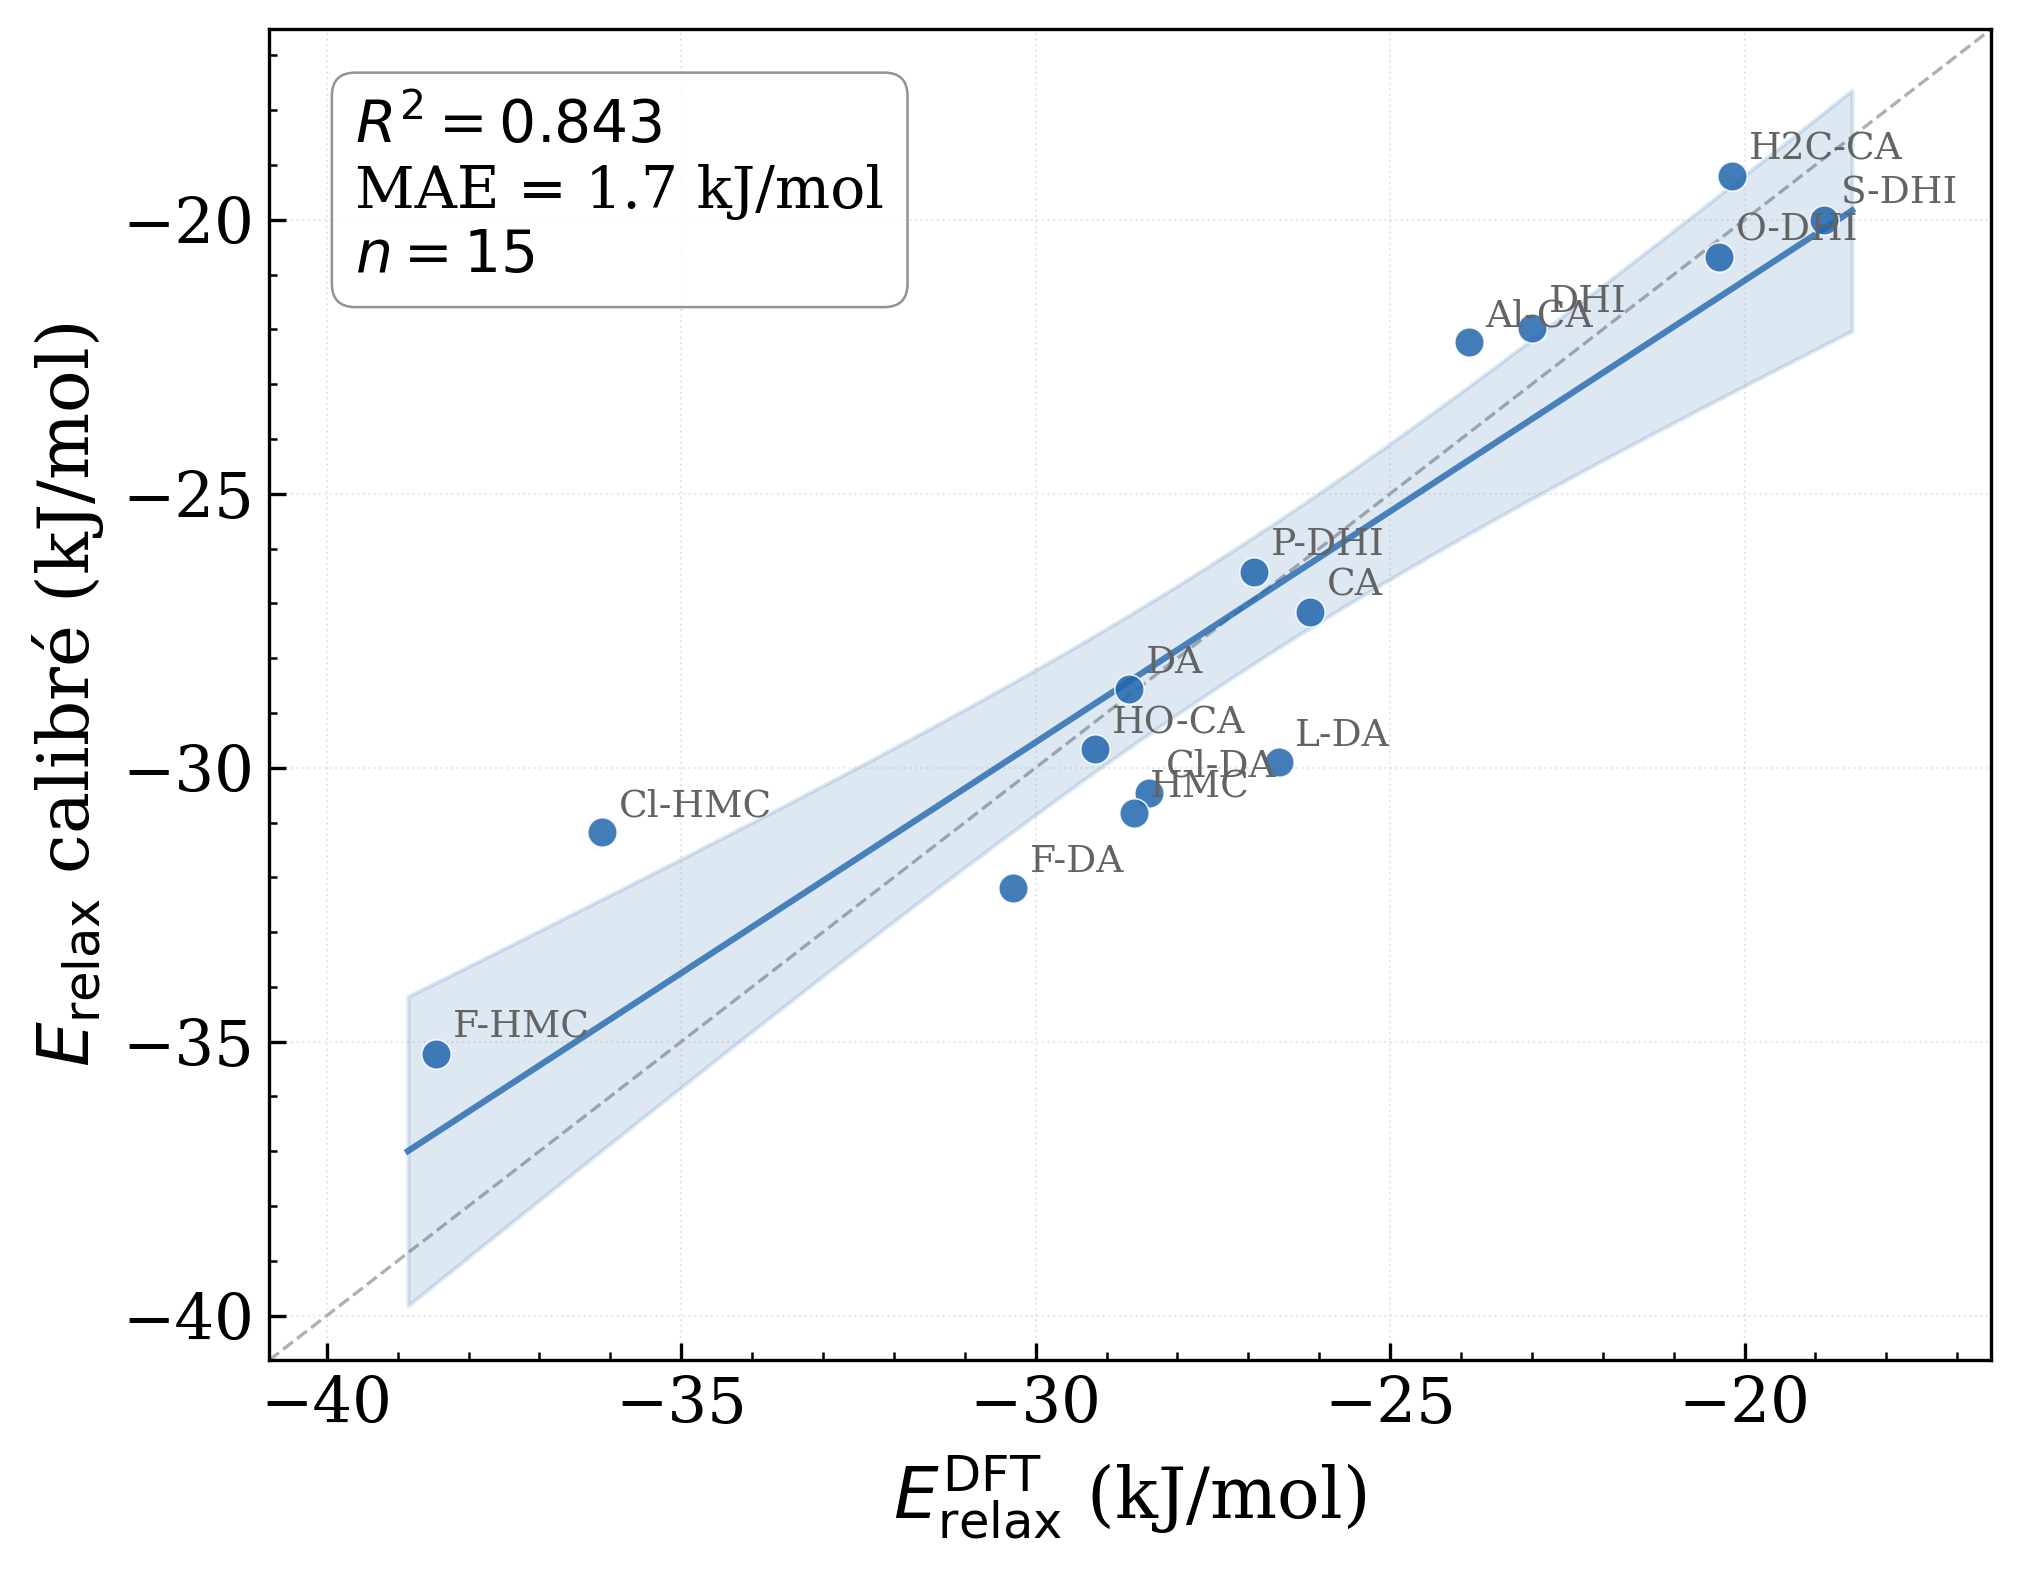
\includegraphics[width=\textwidth]{lvc2_brut_red.png}
\caption{Réduction --- LVC2 brut.}
\label{fig:lvc2_brut}
\end{subfigure}
\hfill
\begin{subfigure}[t]{0.42\textwidth}
\centering
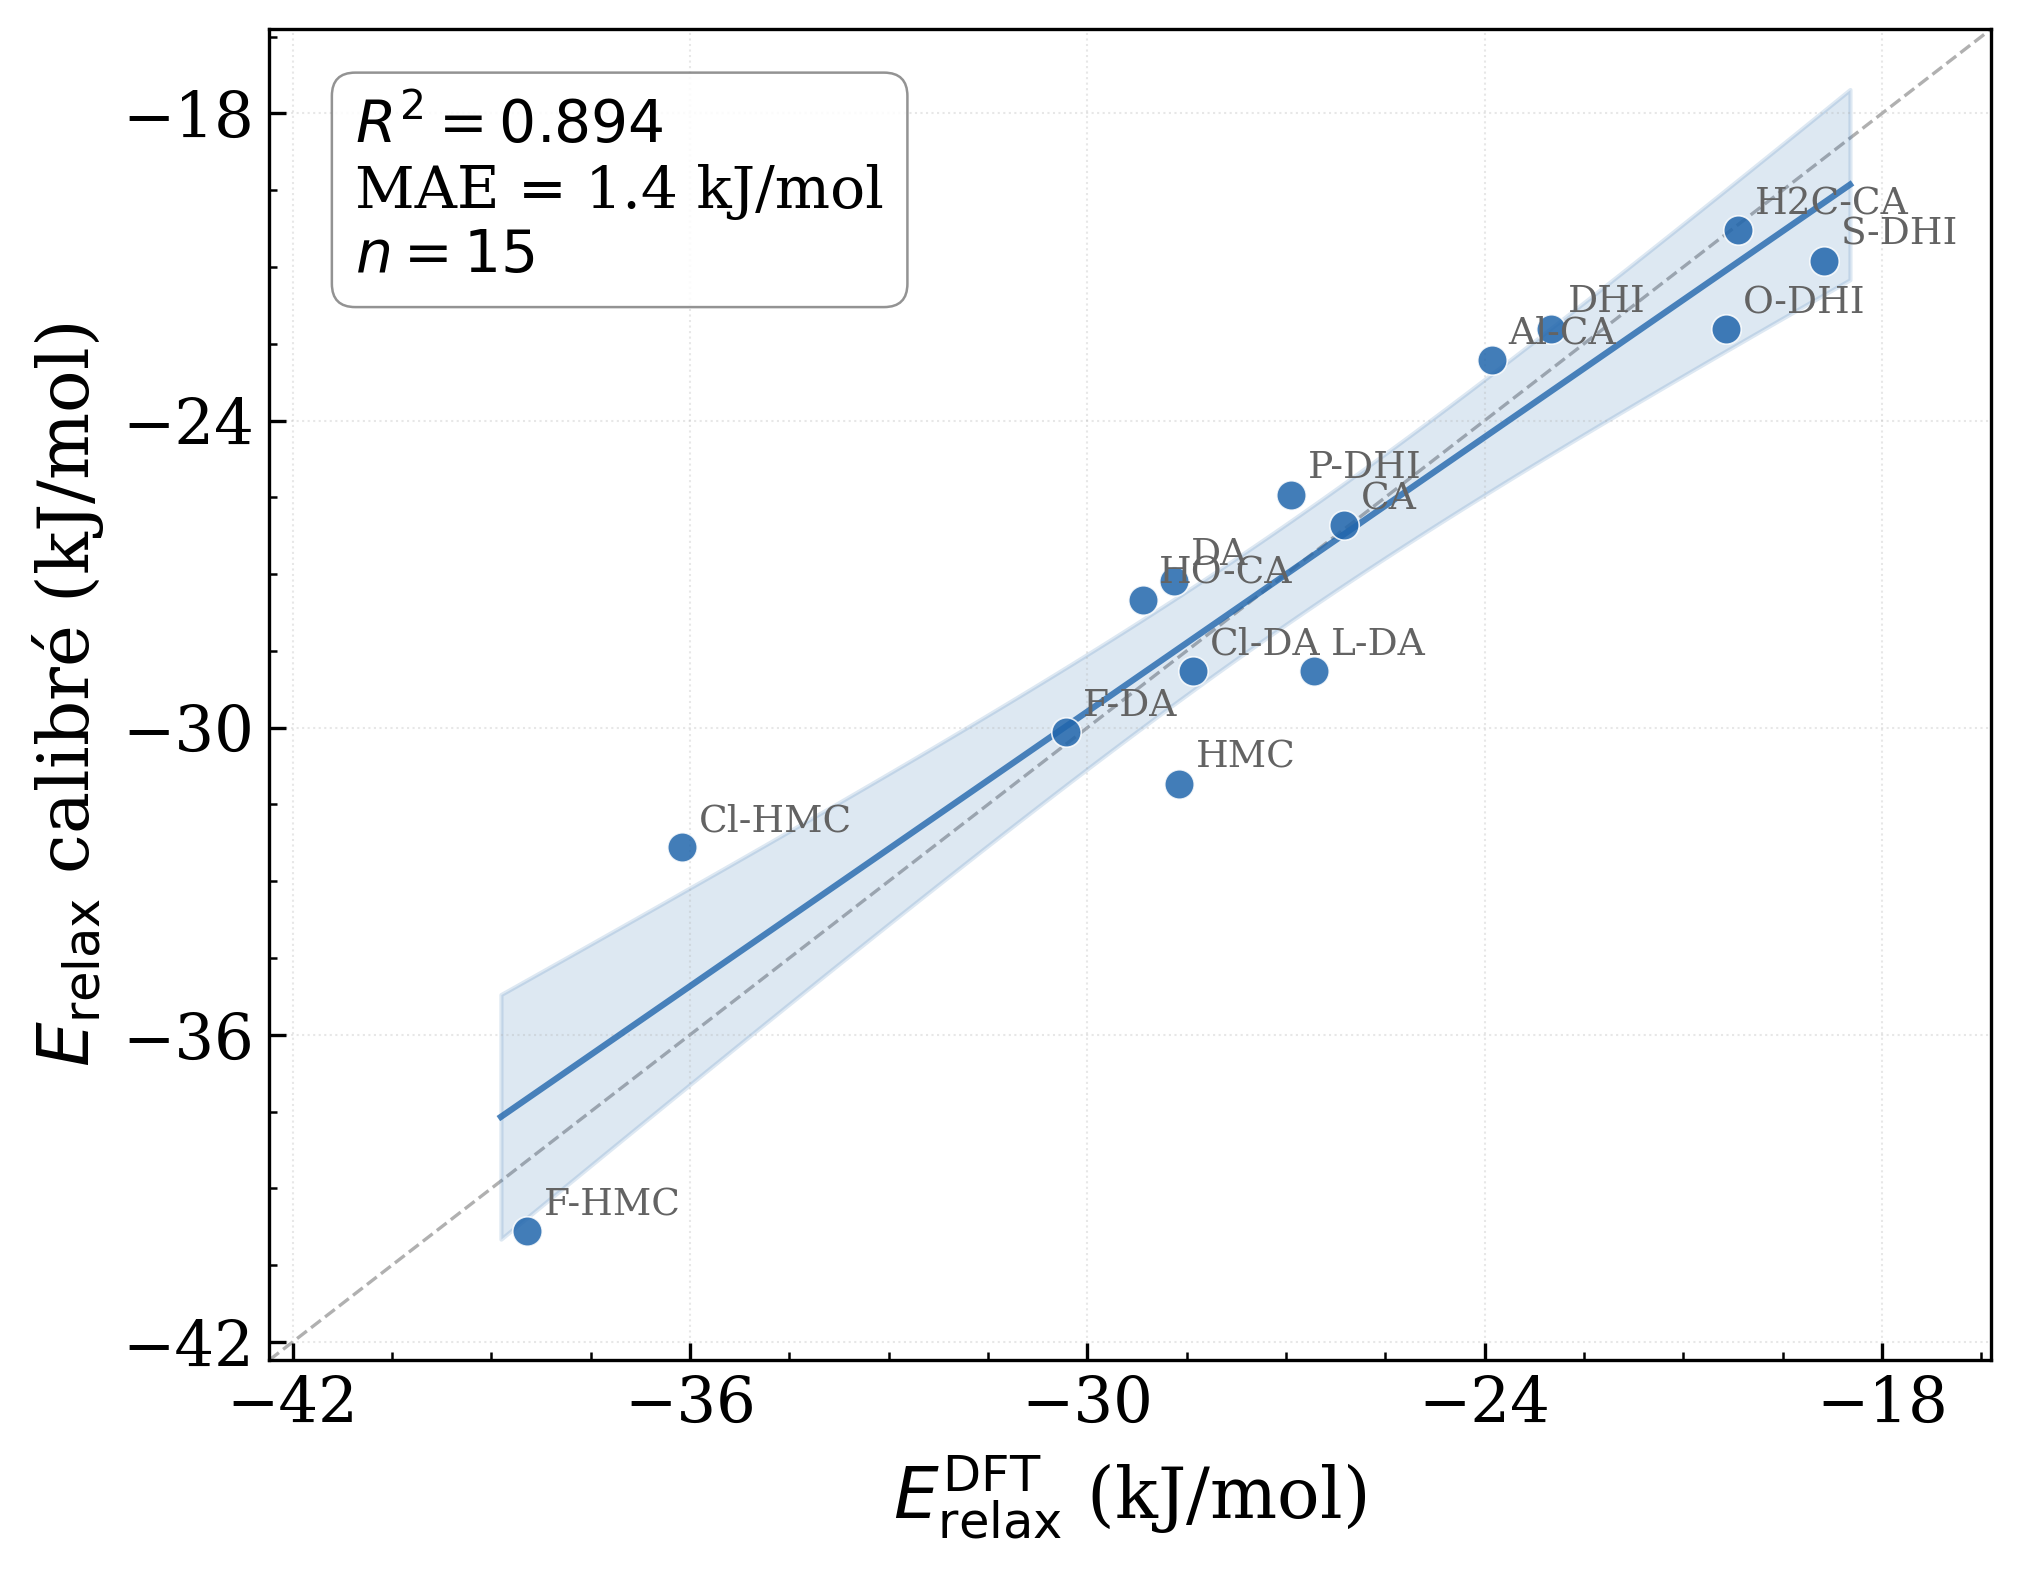
\includegraphics[width=\textwidth]{lvc2_corr_red.png}
\caption{Réduction --- LVC2 corrigé.}
\label{fig:lvc2_corr}
\end{subfigure}
\caption{Effet de la correction LUMO (éq.~\ref{eq:lvc2_corr}) sur la prédiction de $E_{\text{relax}}$. Haut : oxydation, bas : réduction. Gauche : LVC2 brut, droite : LVC2 corrigé. Tous les parity plots sont calibrés. La correction améliore la réduction ($R^2 : 0.84 \to 0.89$) mais pas l'oxydation.}
\label{fig:lvc2_corrected}
\end{figure}

\paragraph{Discussion.}
La correction par $f_{\text{O}}^{\text{LUMO}}$ est efficace mais repose sur une vision mono-orbitale (la LUMO seule) de la redistribution électronique lors de la réduction. Or, la densité de l'électron ajouté ne coïncide pas exactement avec $|\psi_{\text{LUMO}}|^2$ : la relaxation orbitale redistribue la densité sur l'ensemble des orbitales occupées. Cette observation motive l'utilisation des fonctions de Fukui, qui intègrent cette relaxation par construction et constituent la généralisation naturelle de l'approche mono-orbitale à la DFT conceptuelle.

\subsubsection{Correction par les fonctions de Fukui}
\label{sec:fukui_correction}

\paragraph{Théorie.}
La DFT conceptuelle (CDFT) fournit des descripteurs de réactivité fondés sur la réponse de la densité électronique au changement du nombre d'électrons. Les fonctions de Fukui condensées sur les bassins atomiques $A$ sont définies par :
\begin{align}
f_A^+ &= q_A(N) - q_A(N+1) & &\text{(attaque nucléophile, réduction)} \label{eq:fukui_plus} \\
f_A^- &= q_A(N-1) - q_A(N) & &\text{(attaque électrophile, oxydation)} \label{eq:fukui_minus} \\
\Delta f_A &= f_A^+ - f_A^- & &\text{(descripteur dual)} \label{eq:fukui_dual}
\end{align}
où $q_A(N)$ est la charge de Hirshfeld de l'atome $A$ dans le système à $N$ électrons. Contrairement à $f_{\text{O}}^{\text{LUMO}}$ qui ne voit que la LUMO, $f_A^+$ intègre la relaxation orbitale complète lors de l'ajout d'un électron. Plusieurs descripteurs condensés sont envisageables : somme sur les oxygènes ($f_{\text{sumO}}^+$), valeur maximale atomique ($\max_A f_A^+$), ou descripteur dual intégré ($\Delta f_{\text{sumO}}$). Les descripteurs globaux de CDFT --- potentiel chimique $\mu$, dureté $\eta$ et électrophilicité $\omega$ --- sont également testés.

\paragraph{Résultats.}
Chaque processus redox est analysé avec la fonction de Fukui physiquement pertinente : $f^+$ pour la réduction (ajout d'électron) et $f^-$ pour l'oxydation (retrait d'électron).

\emph{Réduction.} La figure~\ref{fig:fukui_red} montre les corrélations entre le résidu LVC2 en réduction et les descripteurs $f^+$ ($n = 13$ molécules). La Fukui $f^+_{\text{sumO}}$ corrèle significativement avec le résidu ($r = -0.67$, $p = 0.012$), tout comme le descripteur dual $\Delta f_{\text{sumO}}$ ($r = -0.69$, $p = 0.009$). Ces performances sont comparables à celle de $f_{\text{O}}^{\text{LUMO}}$ ($R^2 = 0.47$).

\begin{figure}[H]
\centering
\begin{subfigure}[t]{0.32\textwidth}
\centering
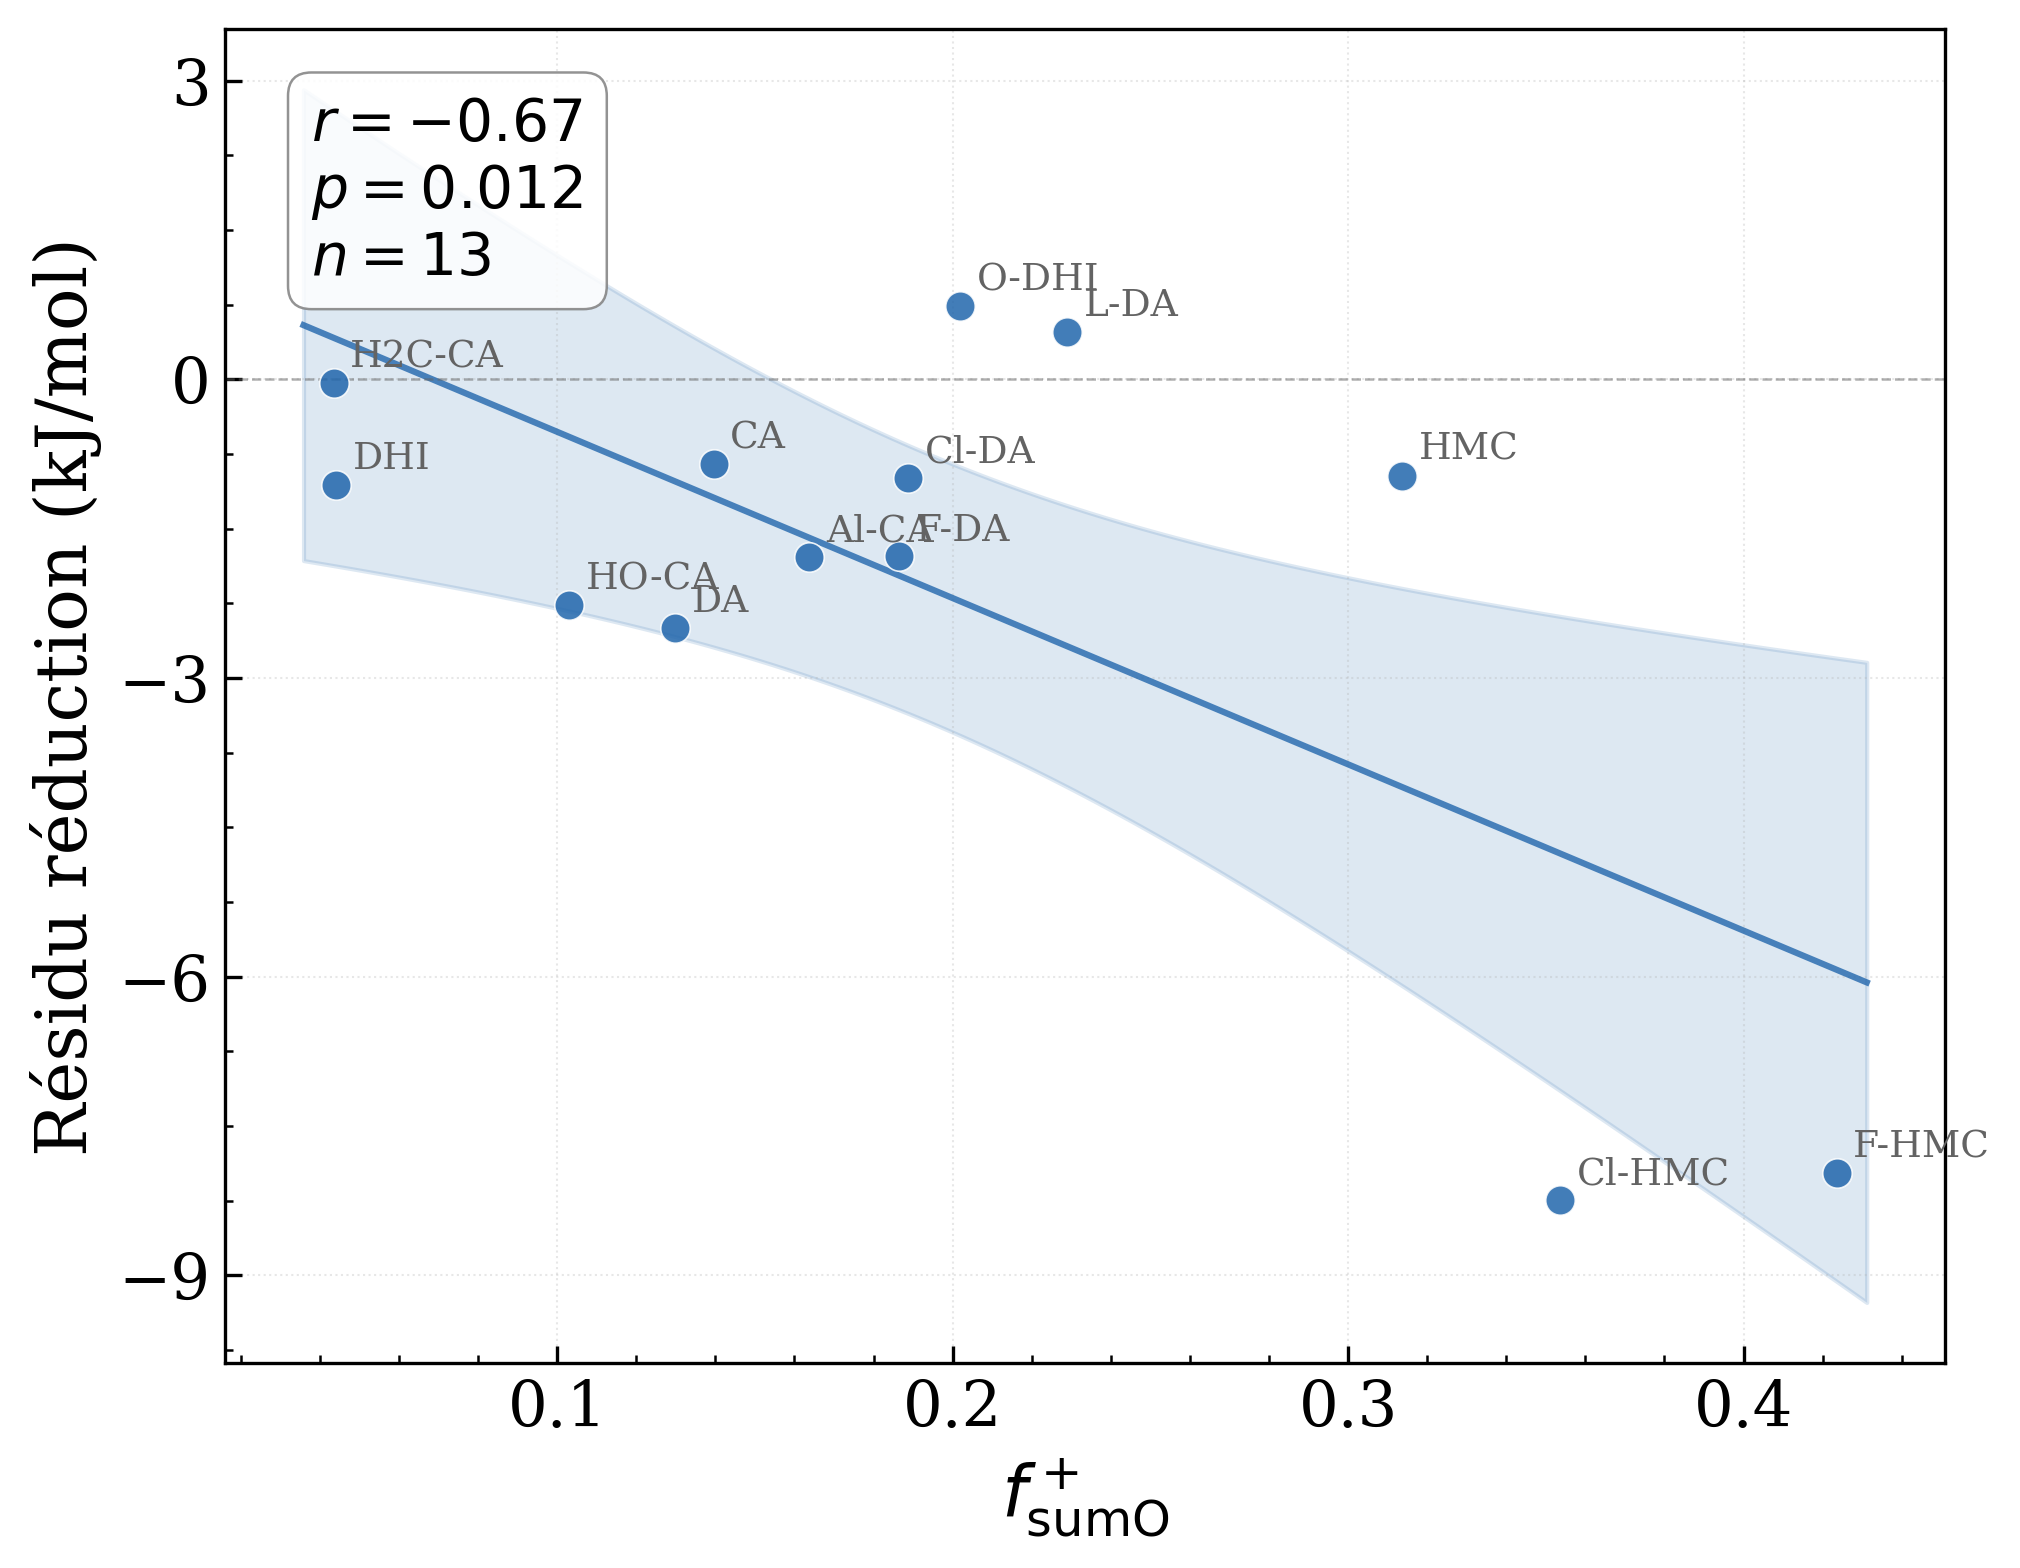
\includegraphics[width=\textwidth]{fukui_fplus_sumO_red.png}
\caption{$f^+_{\text{sumO}}$ ($r = -0.67$, $p = 0.012$).}
\label{fig:fukui_fplus_red}
\end{subfigure}
\hfill
\begin{subfigure}[t]{0.32\textwidth}
\centering
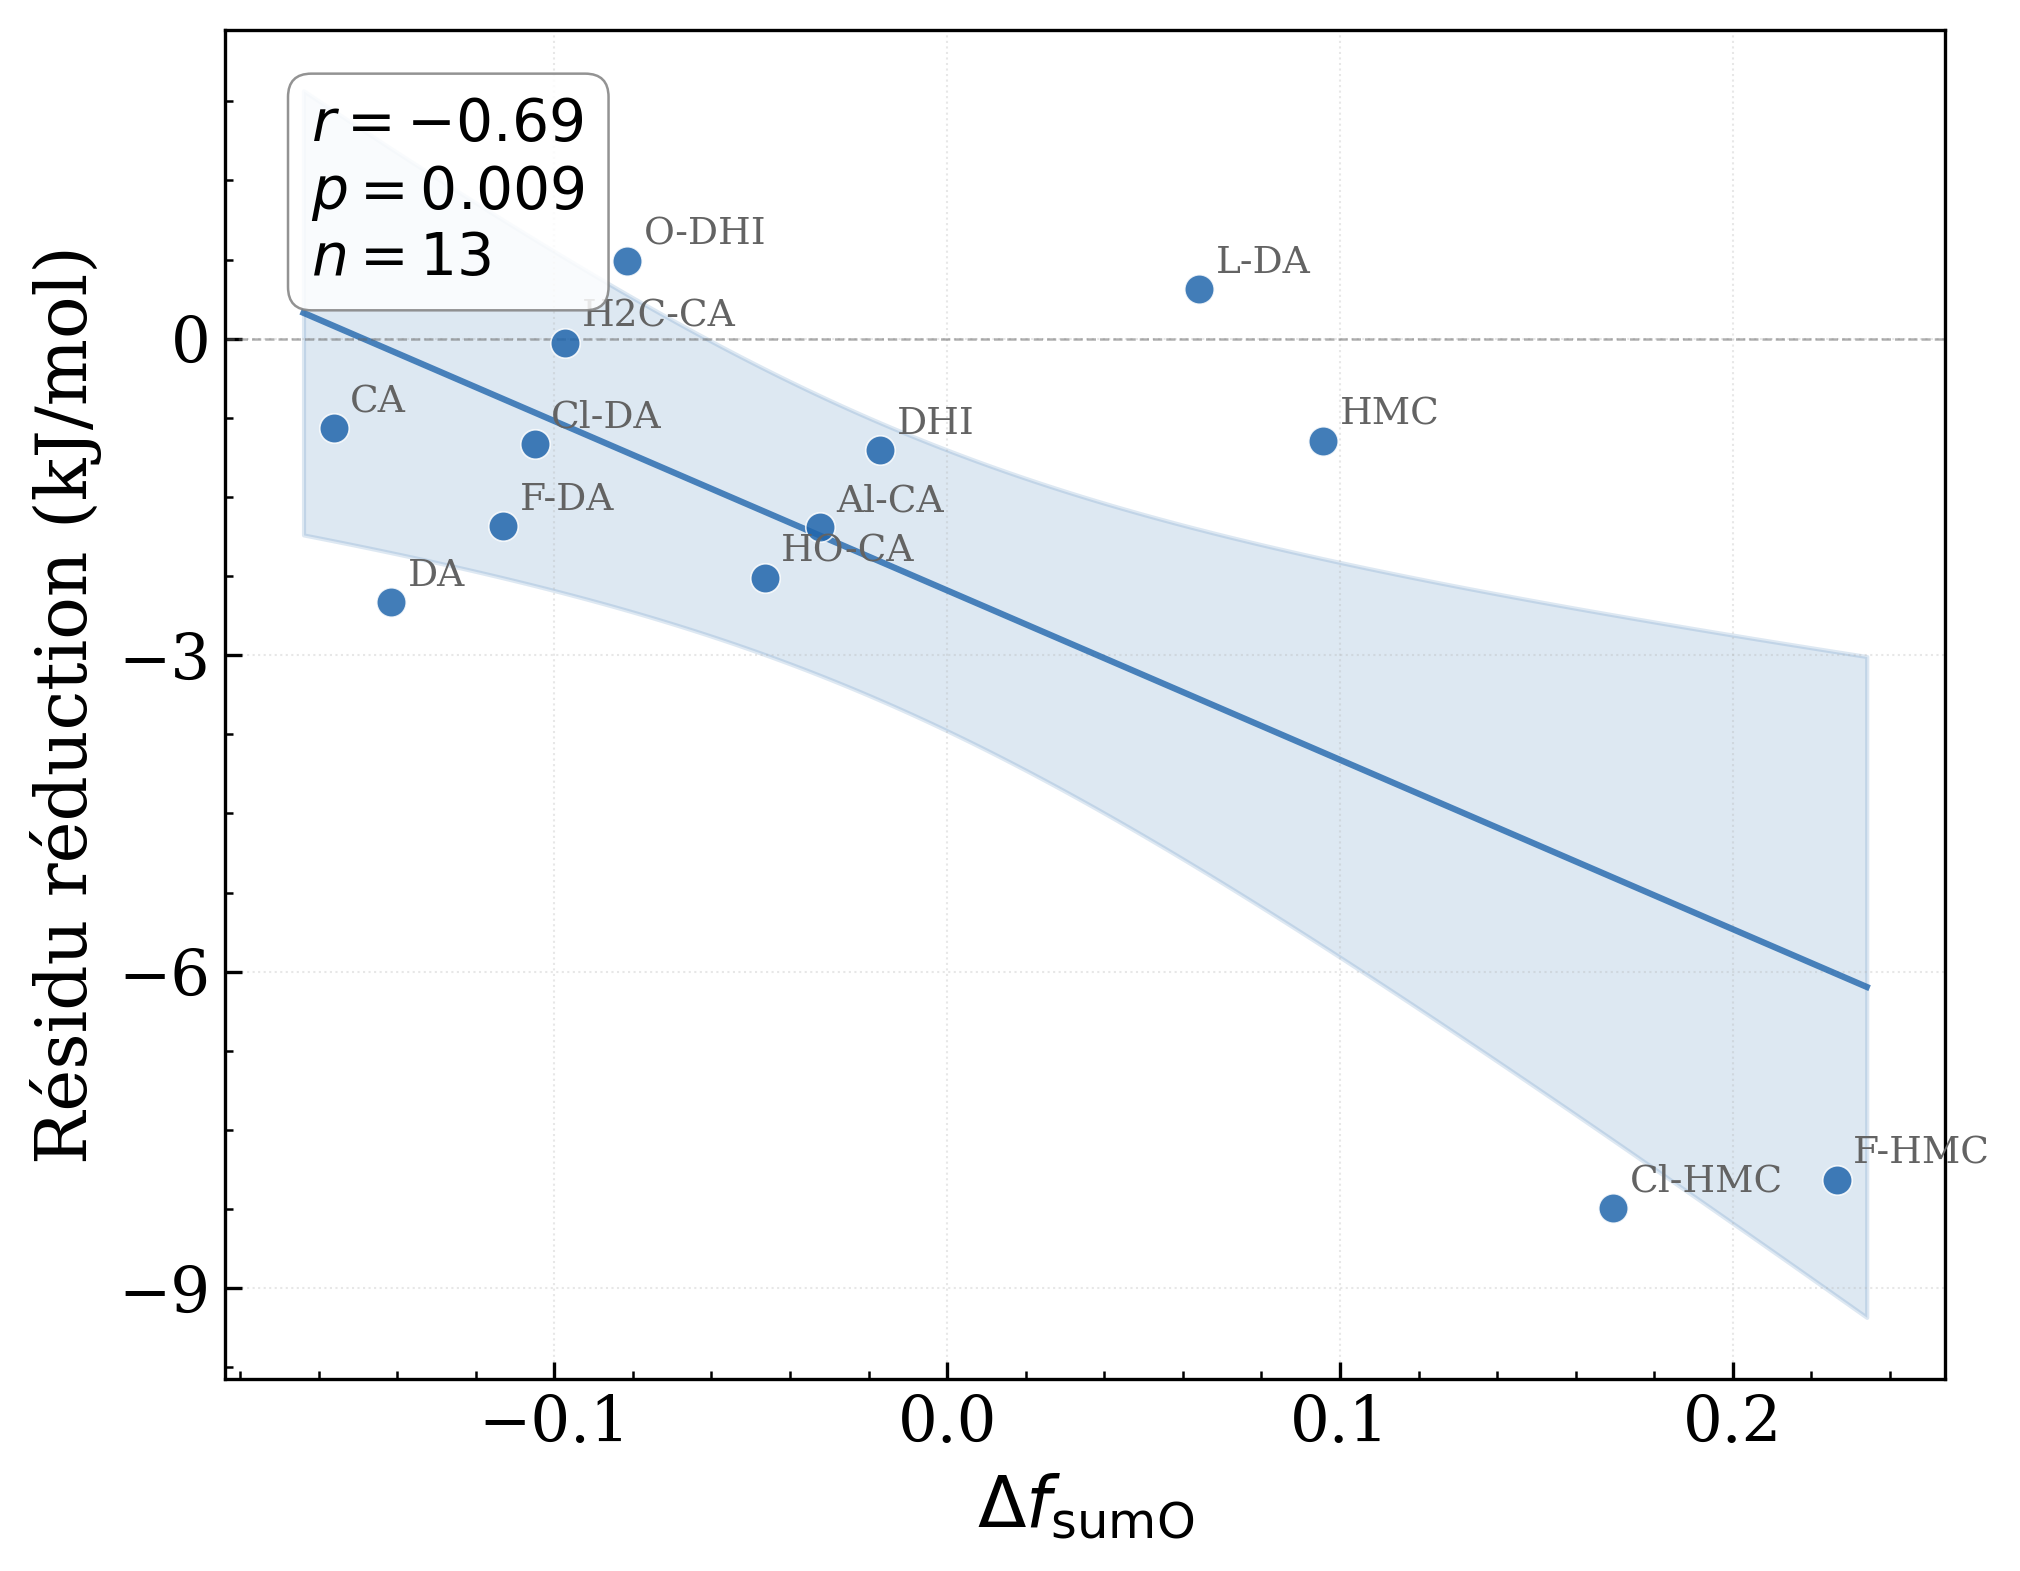
\includegraphics[width=\textwidth]{fukui_dual_sumO_red.png}
\caption{$\Delta f_{\text{sumO}}$ ($r = -0.69$, $p = 0.009$).}
\label{fig:fukui_dual_red}
\end{subfigure}
\hfill
\begin{subfigure}[t]{0.32\textwidth}
\centering
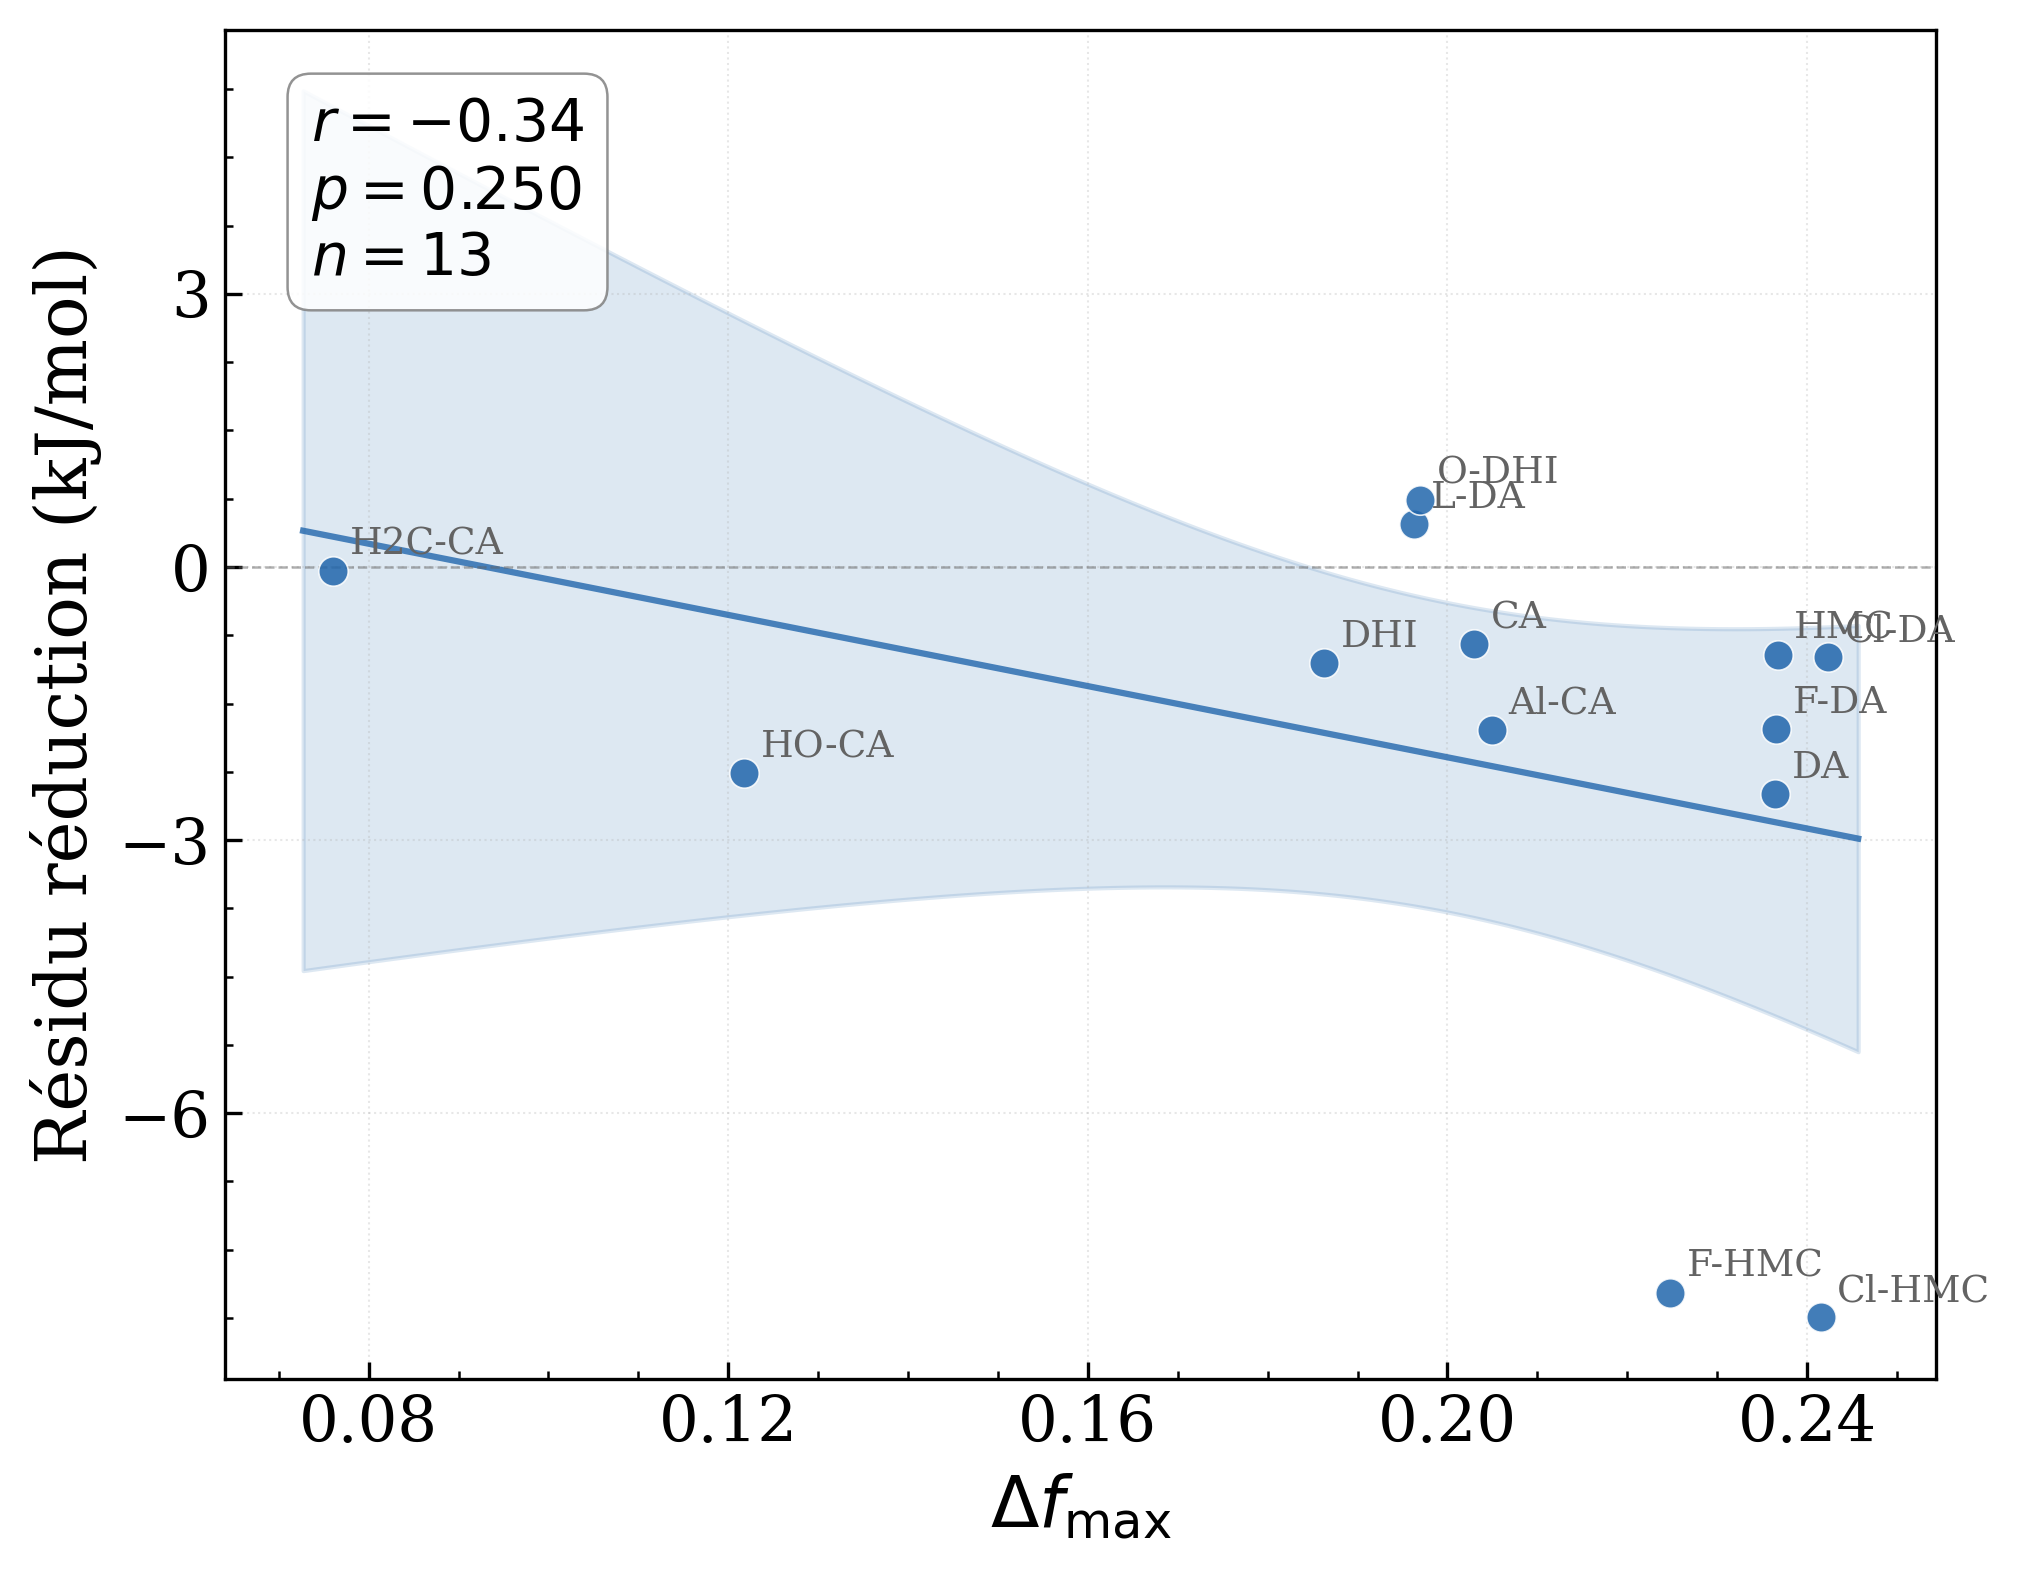
\includegraphics[width=\textwidth]{fukui_dual_max_red.png}
\caption{$\Delta f_{\max}$ ($r = -0.34$, $p = 0.25$).}
\label{fig:fukui_dmax_red}
\end{subfigure}
\caption{Résidu LVC2 en réduction vs descripteurs de Fukui ($n = 13$). (a)~$f^+_{\text{sumO}}$ et (b)~$\Delta f_{\text{sumO}}$ corrèlent significativement. (c)~Le descripteur dual atomique maximal $\Delta f_{\max}$ n'est pas significatif.}
\label{fig:fukui_red}
\end{figure}

\emph{Oxydation.} La figure~\ref{fig:fukui_ox} montre les corrélations avec les descripteurs $f^-$. Aucune corrélation significative n'est observée, ni pour $f^-_{\text{sumO}}$ ($r = -0.16$, $p = 0.59$), ni pour le descripteur dual intégré ($r = -0.35$, $p = 0.25$), ni pour $\Delta f_{\min}$ ($r = 0.39$, $p = 0.19$). Ce résultat est cohérent avec la faiblesse du résidu LVC2 en oxydation (MAE brute $= \SI{1.4}{kJ/mol}$) : le LVC2 prédit déjà $E_{\text{relax}}$ avec une précision quasi-optimale, ne laissant pas de résidu structuré à corriger.

\begin{figure}[H]
\centering
\begin{subfigure}[t]{0.32\textwidth}
\centering
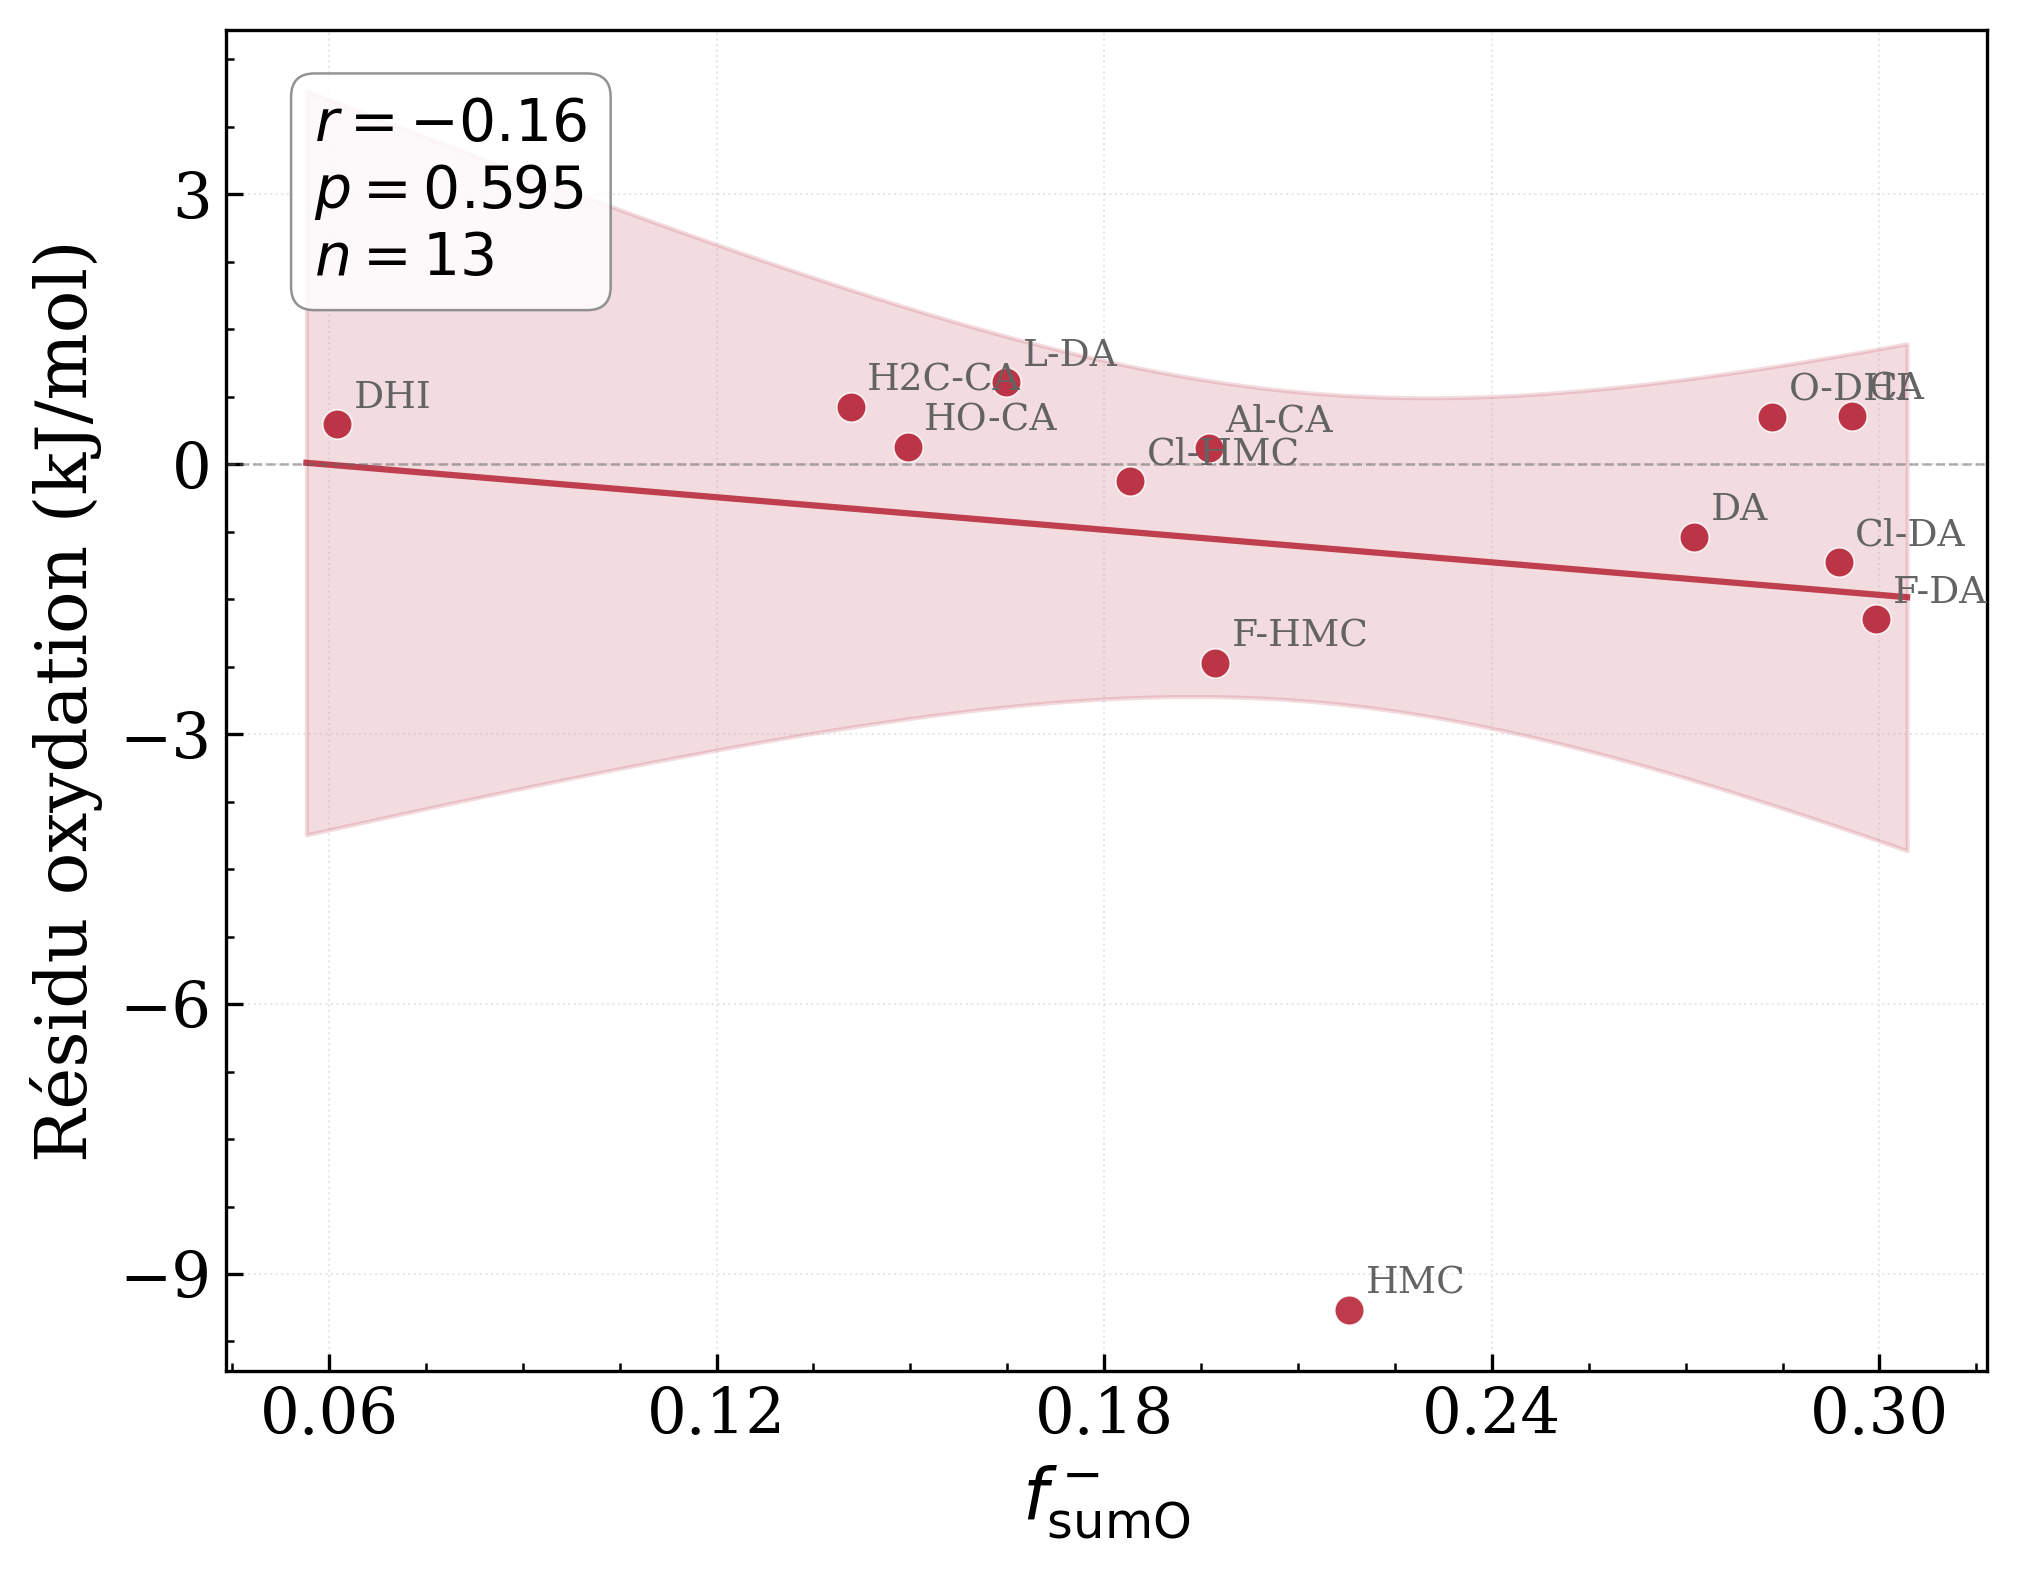
\includegraphics[width=\textwidth]{fukui_fminus_sumO_ox.png}
\caption{$f^-_{\text{sumO}}$ ($r = -0.16$, $p = 0.59$).}
\label{fig:fukui_fminus_ox}
\end{subfigure}
\hfill
\begin{subfigure}[t]{0.32\textwidth}
\centering
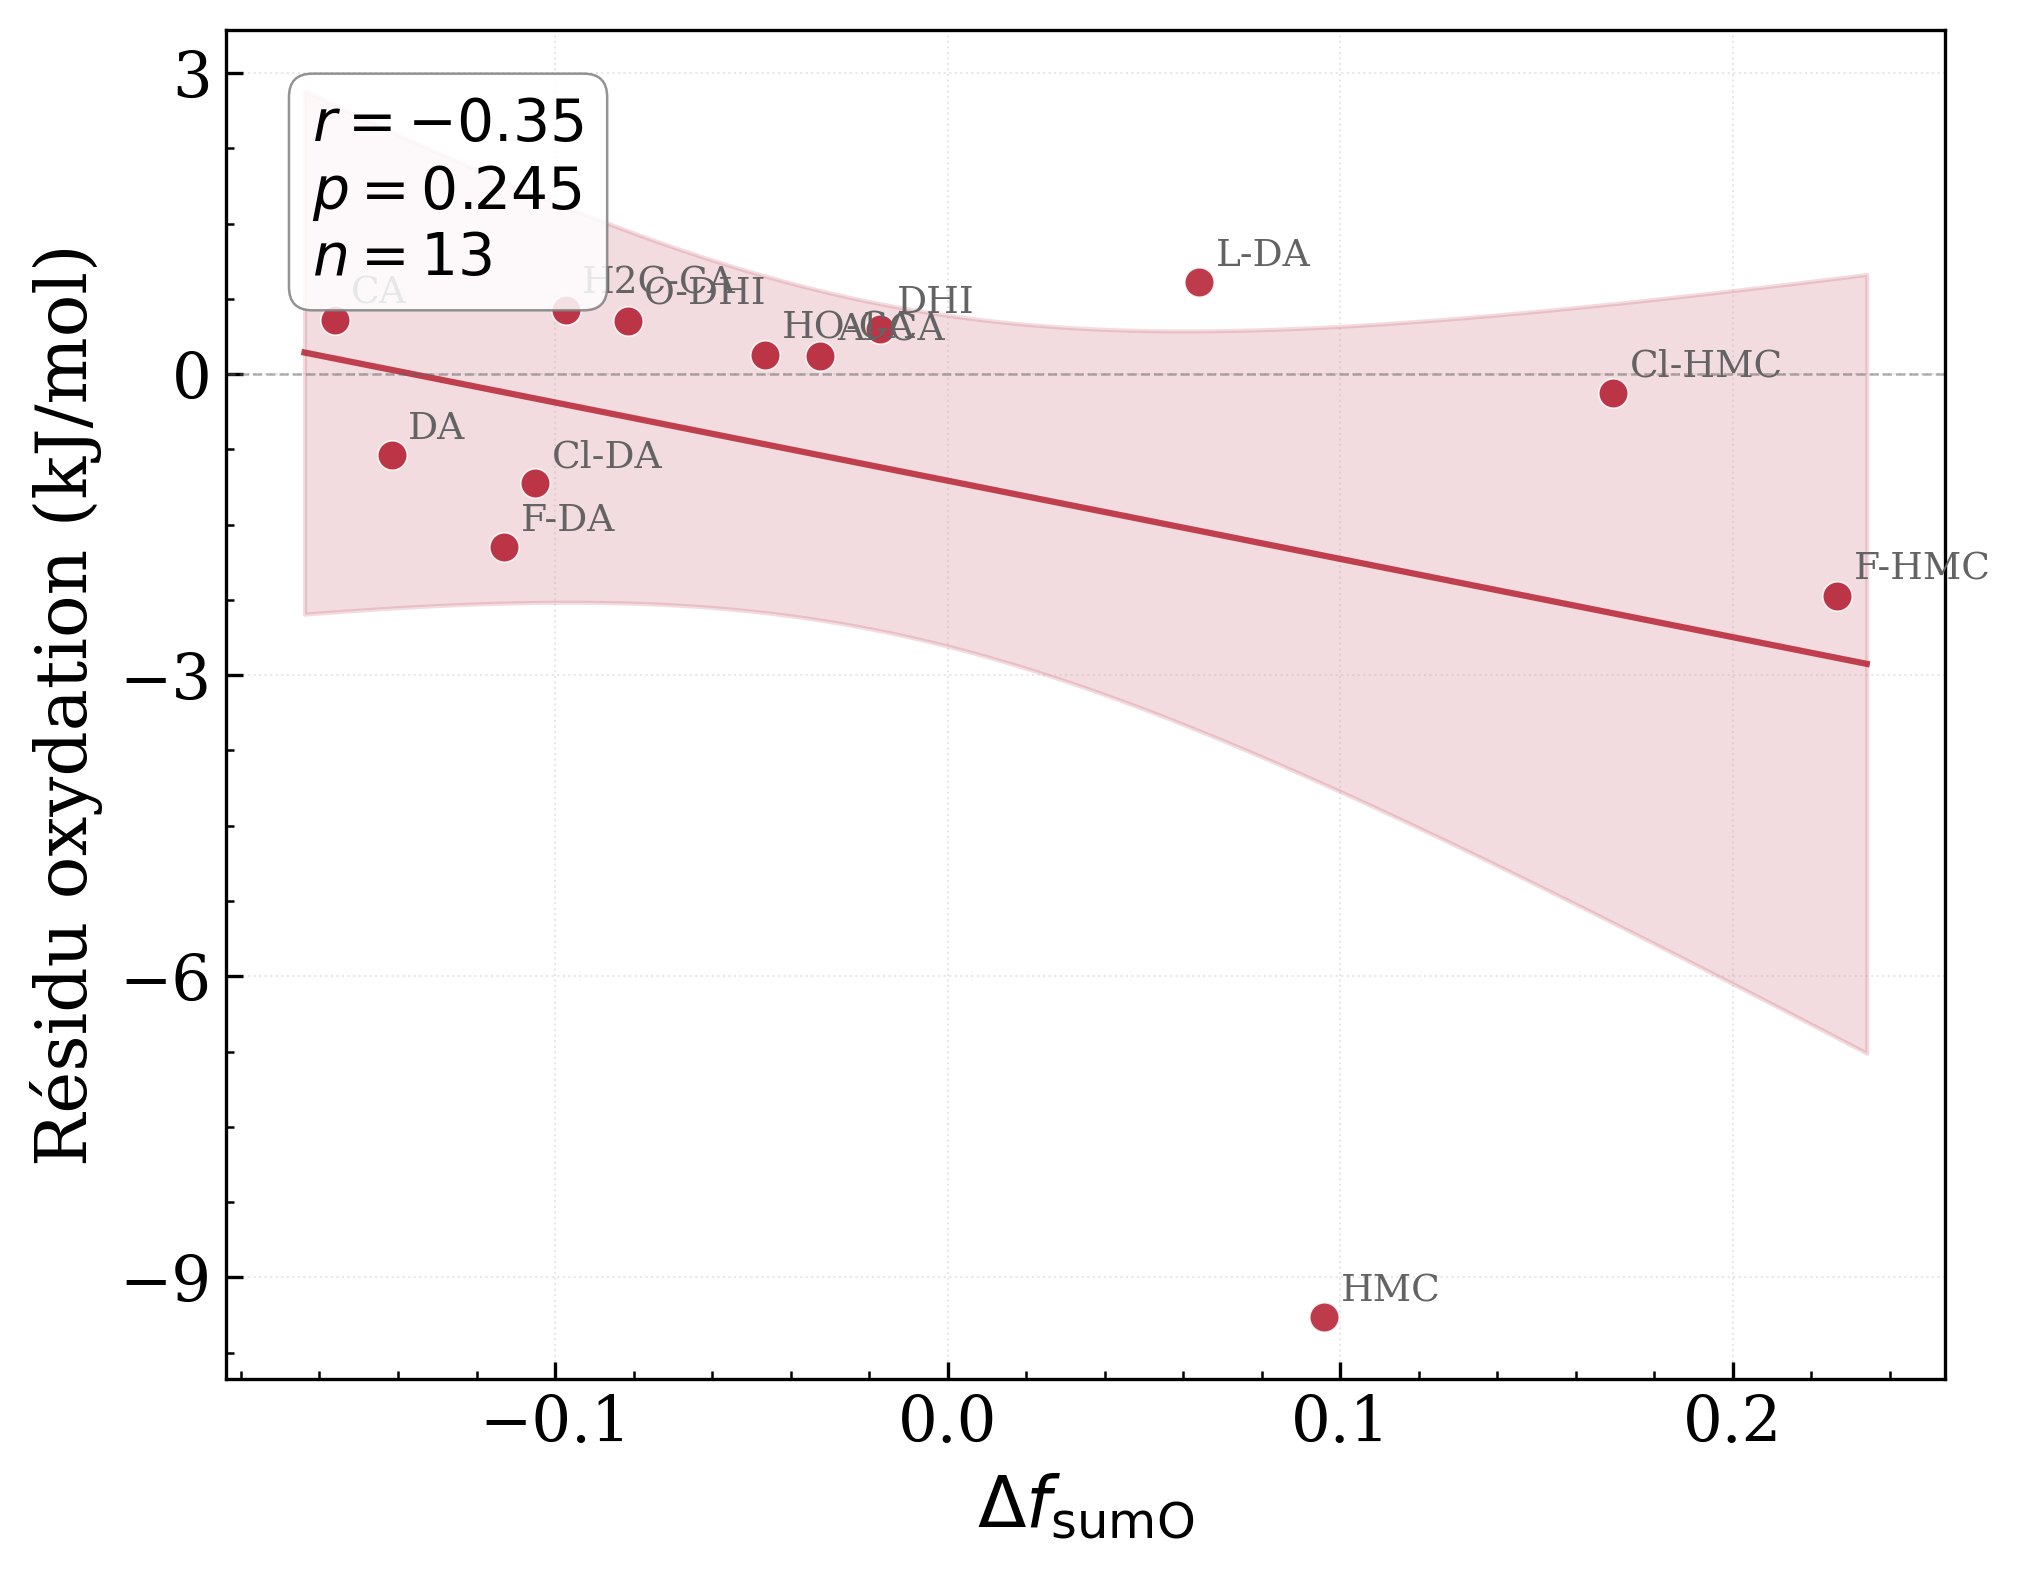
\includegraphics[width=\textwidth]{fukui_dual_sumO_ox.png}
\caption{$\Delta f_{\text{sumO}}$ ($r = -0.35$, $p = 0.25$).}
\label{fig:fukui_dual_ox}
\end{subfigure}
\hfill
\begin{subfigure}[t]{0.32\textwidth}
\centering
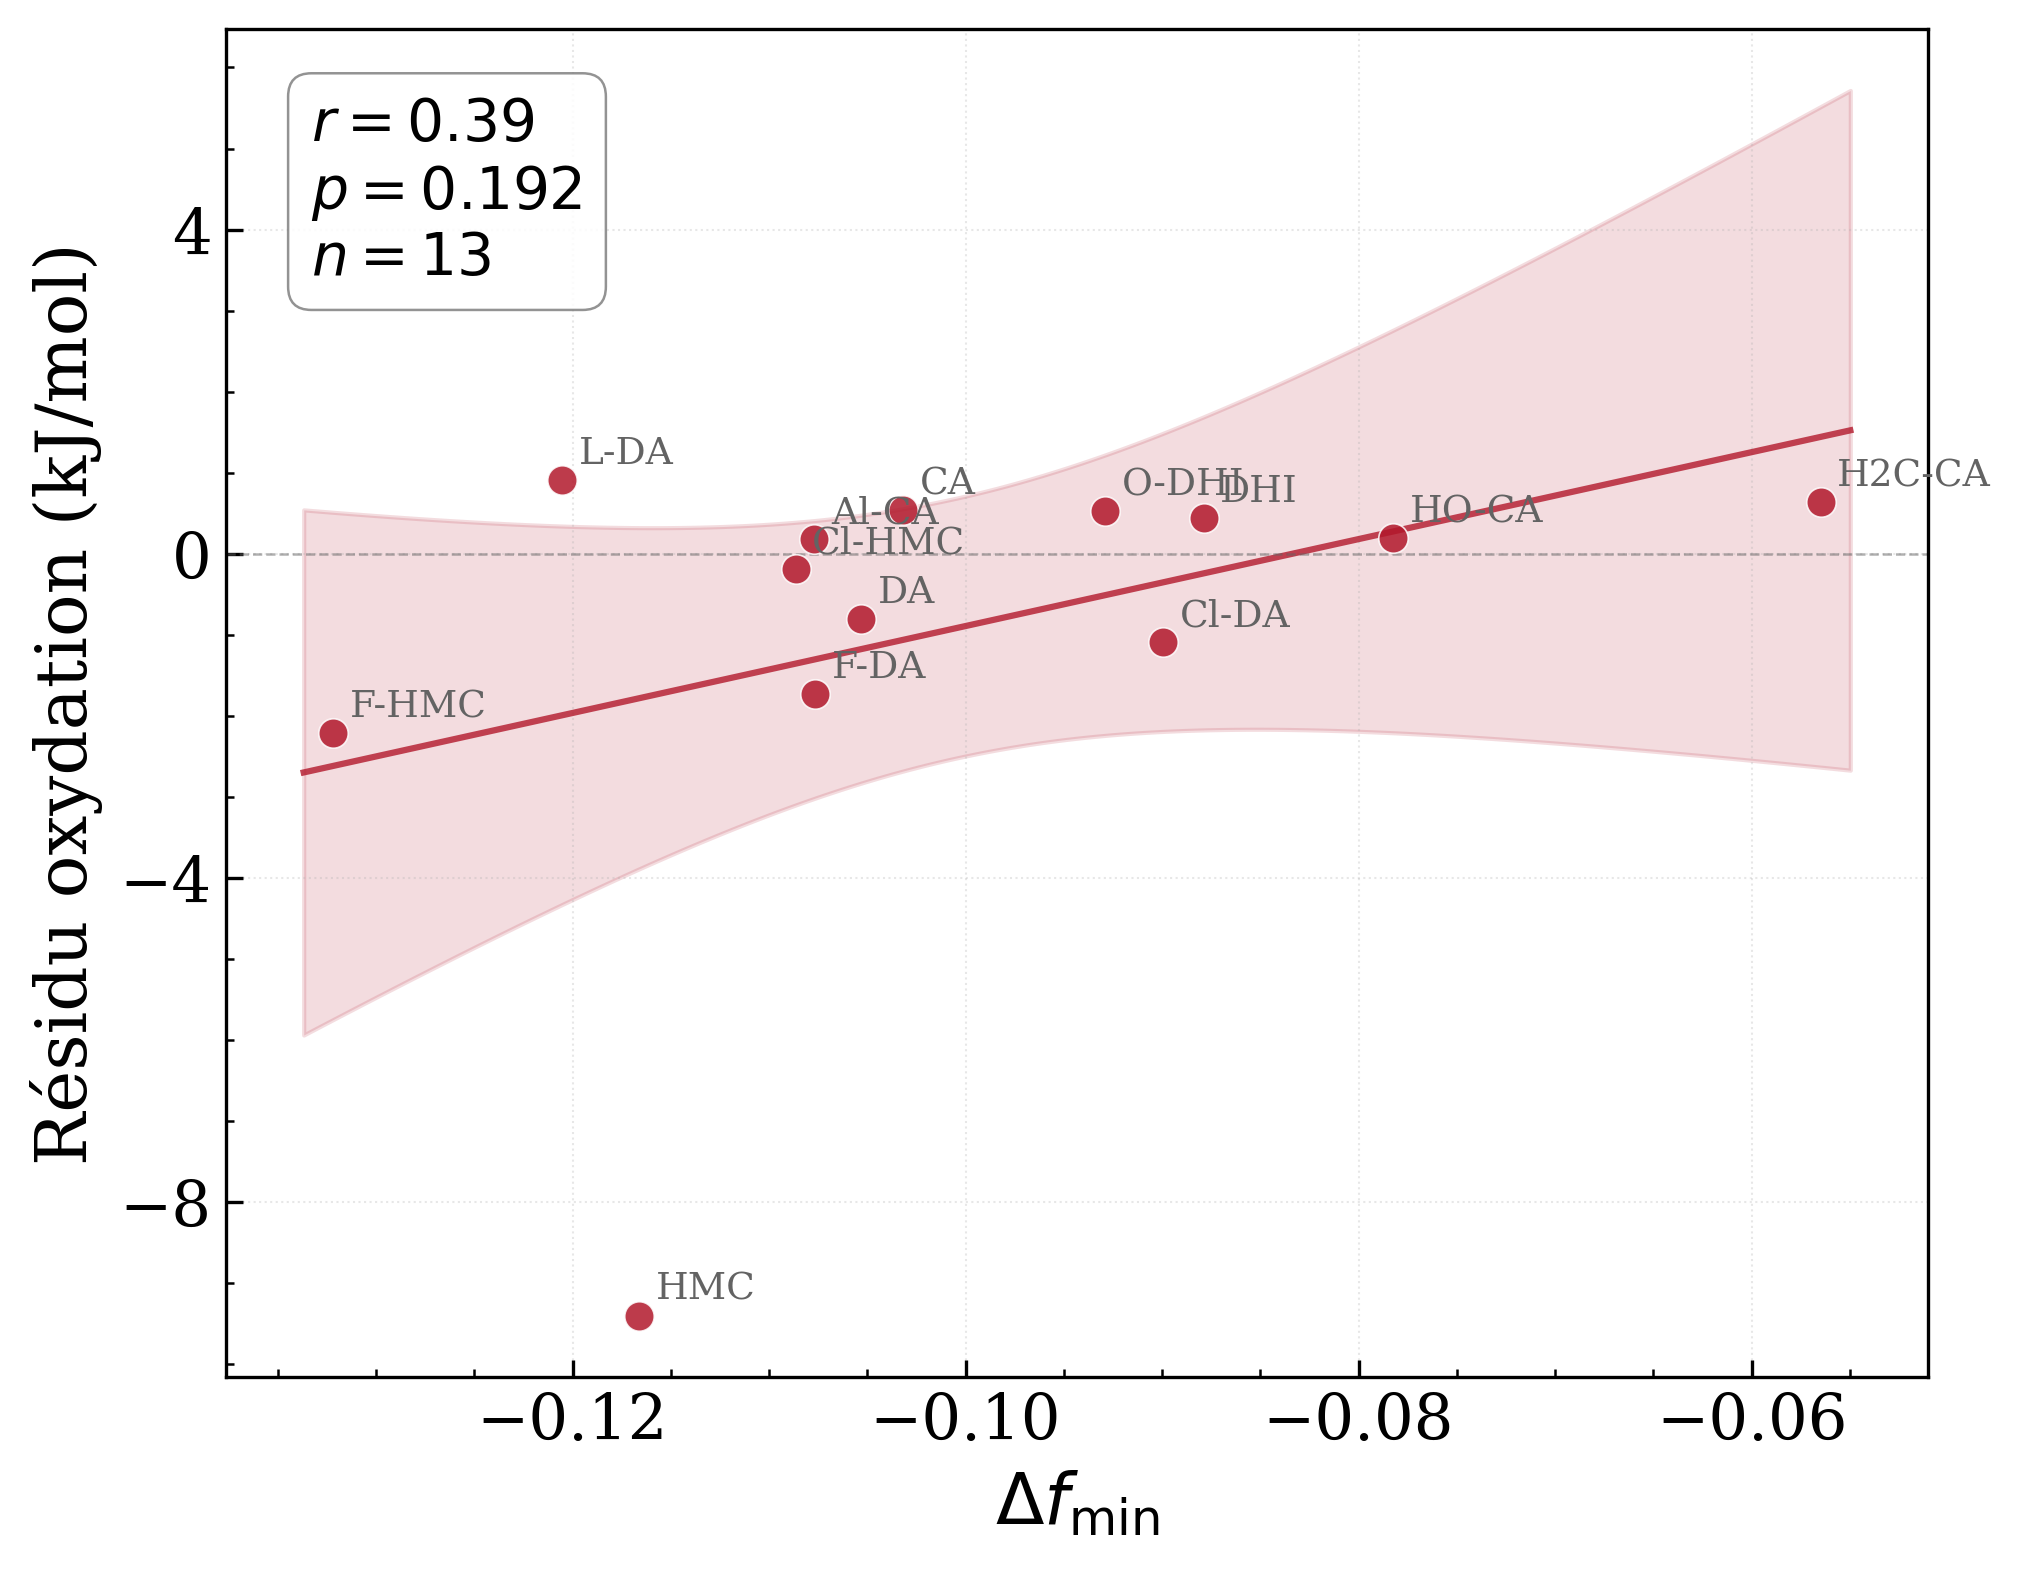
\includegraphics[width=\textwidth]{fukui_dual_min_ox.png}
\caption{$\Delta f_{\min}$ ($r = 0.39$, $p = 0.19$).}
\label{fig:fukui_dmin_ox}
\end{subfigure}
\caption{Résidu LVC2 en oxydation vs descripteurs de Fukui ($n = 13$). Aucune corrélation significative. Le résidu en oxydation est trop faible pour être corrélé.}
\label{fig:fukui_ox}
\end{figure}

La quasi-identité des performances entre $f^+_{\text{sumO}}$ et $f_{\text{O}}^{\text{LUMO}}$ en réduction suggère une redondance entre ces descripteurs. La figure~\ref{fig:fukui_vs_lumo} le confirme : les deux sont quasi-parfaitement corrélés ($r = 0.98$, $p < 10^{-4}$). Malgré leurs définitions différentes --- $f_{\text{O}}^{\text{LUMO}}$ ne voit que la LUMO par analyse SFO, tandis que $f^+_{\text{sumO}}$ intègre la relaxation orbitale complète par différences finies de charges --- les deux descripteurs encodent la même information physique sur cette série de catéchols.

\begin{figure}[H]
\centering
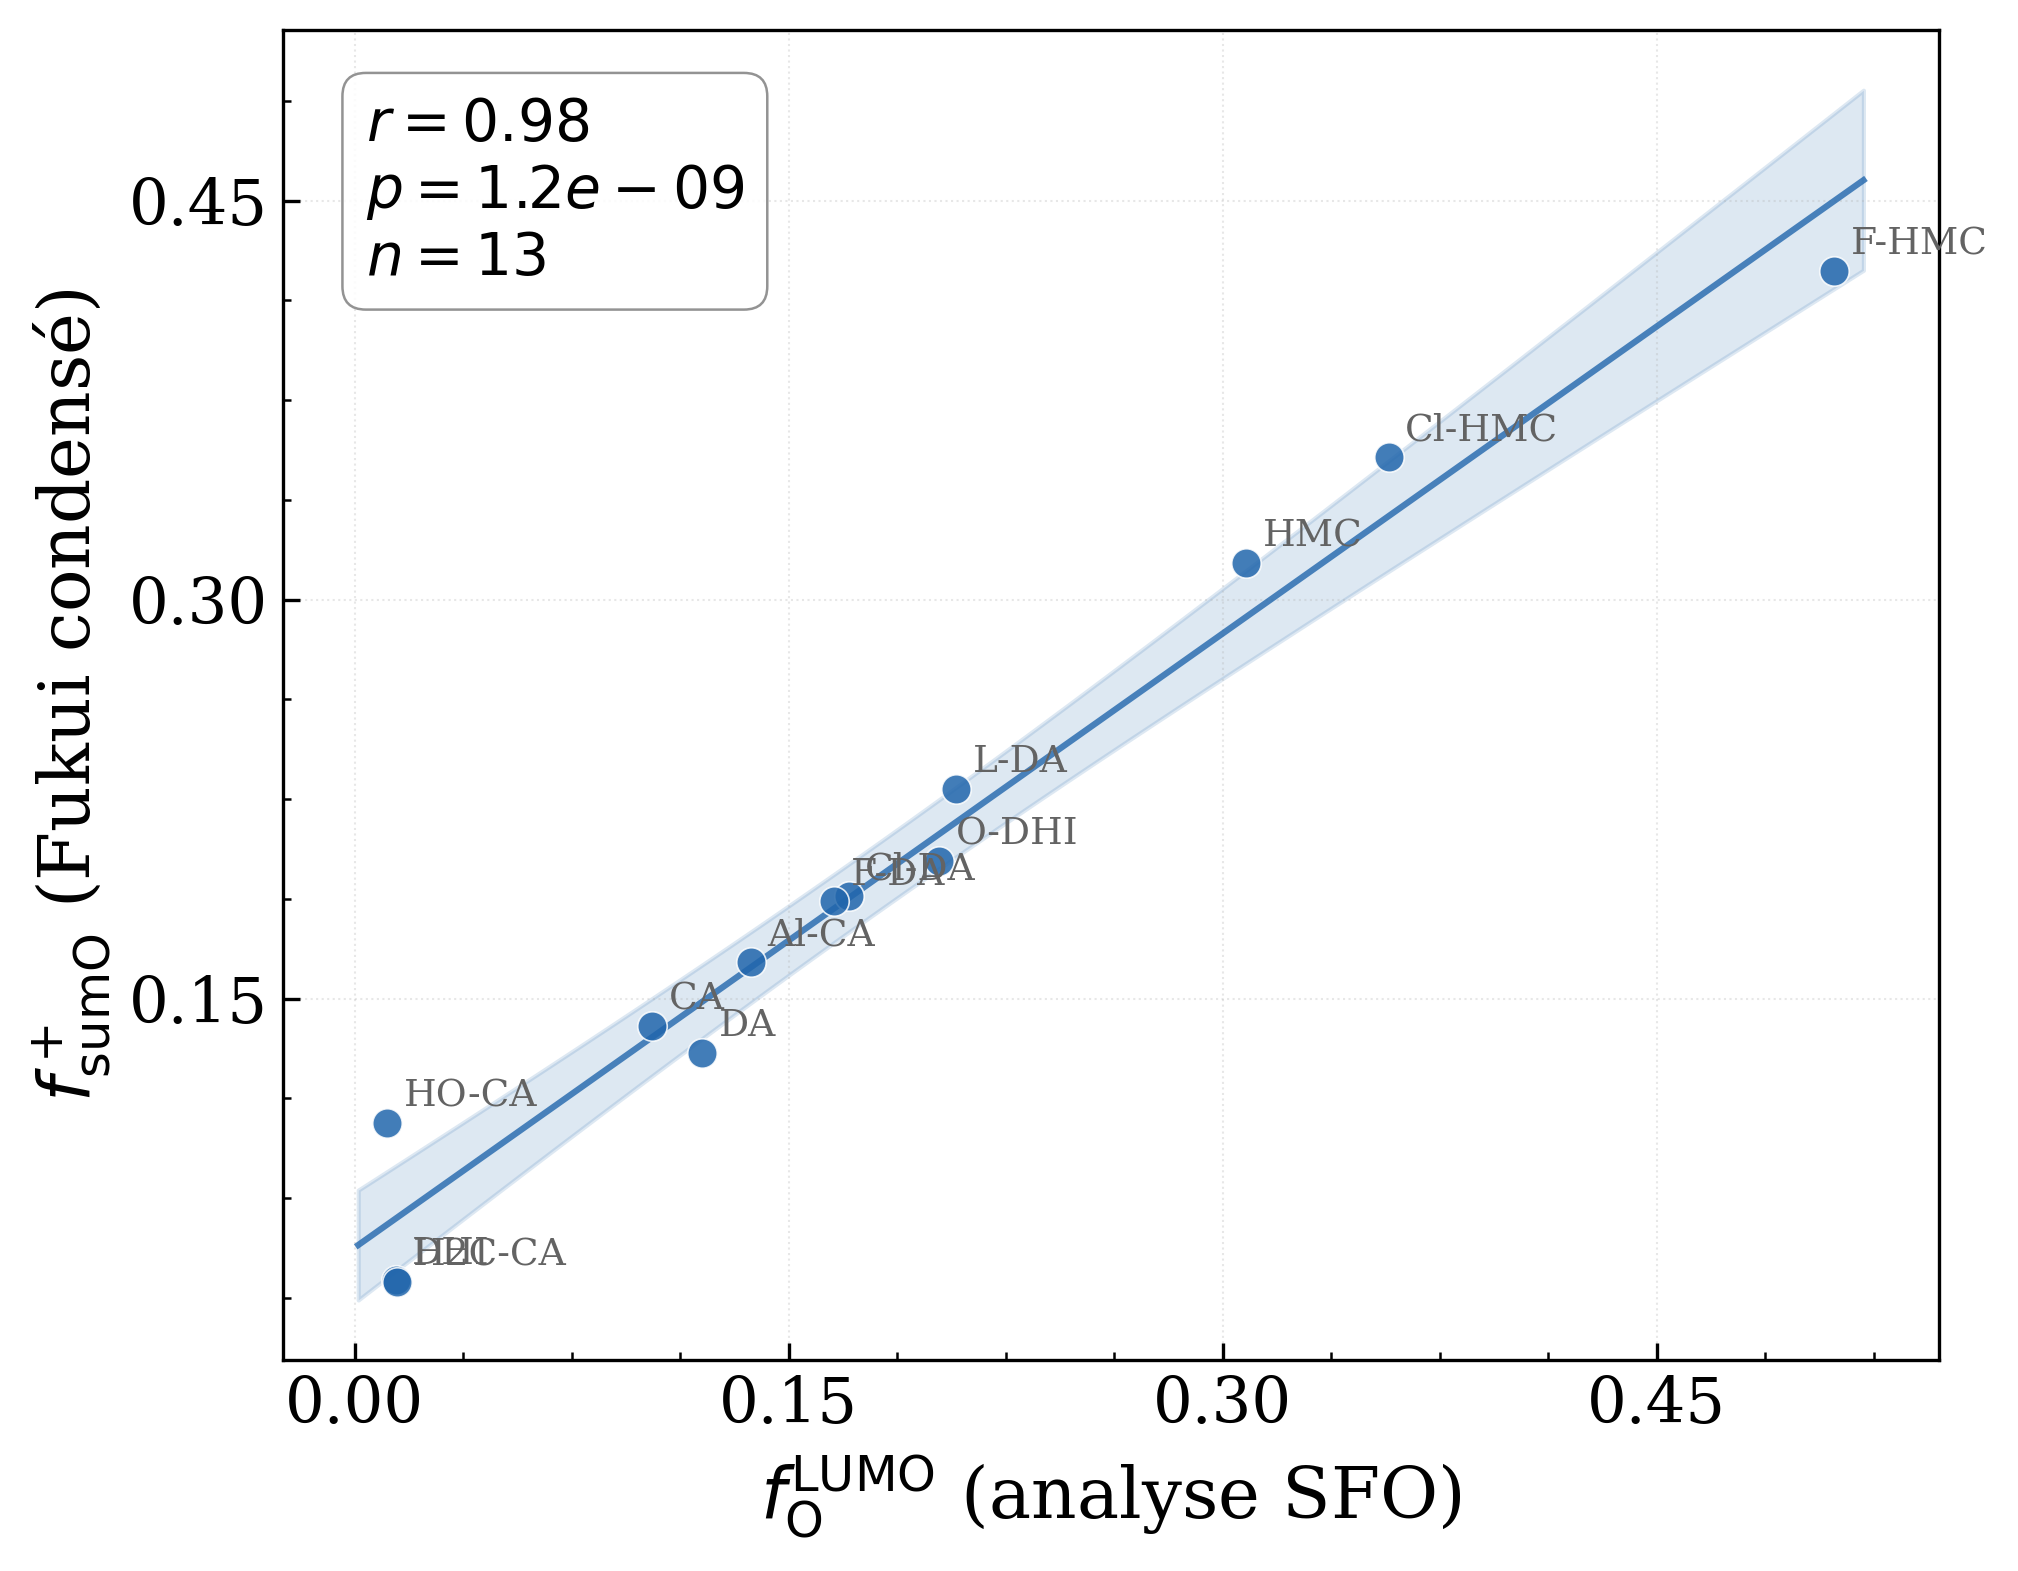
\includegraphics[width=0.55\textwidth]{fukui_vs_lumo_comparison.png}
\caption{Corrélation entre $f^+_{\text{sumO}}$ (Fukui condensé) et $f_{\text{O}}^{\text{LUMO}}$ (analyse SFO). La corrélation quasi-parfaite ($r = 0.98$) démontre la redondance des deux descripteurs sur cette série chimiquement homogène.}
\label{fig:fukui_vs_lumo}
\end{figure}

\paragraph{Modèle symétrique $f^{\pm}_{\max,\text{O}}$.}
Les analyses précédentes montrent que le résidu LVC2 est contrôlé par la distribution \emph{locale} de la densité de Fukui sur les oxygènes. Les descripteurs globaux de CDFT ($\mu$, $\eta$, $\omega$) ne corrèlent avec aucun des deux résidus ($R^2 < 0.09$), et les descripteurs atomiques non ciblés ($\Delta f_{\max}$, $\Delta f_{\min}$, top-$k$ atomiques) sont tous non significatifs (tableau~\ref{tab:fukui_exhaustive}, annexe~\ref{app:fukui}). Seuls les descripteurs intégrés sur les oxygènes portent un signal, ce qui confirme que les deux processus redox de la série catéchol sont gouvernés par les oxygènes du cycle.

Cette observation motive un modèle symétrique utilisant $f^+_{\max,\text{O}} = \max_A f_A^+$ (sur les O) pour la réduction et $f^-_{\max,\text{O}} = \max_A f_A^-$ pour l'oxydation. Le modèle sans paramètre libre :
\begin{equation}
E_{\text{relax}}^{\text{corr}} = E_{\text{relax}}^{\text{LVC2}} \times \left(1 + \left|f^{\pm}_{\max,\text{O}}\right|^{3/2}\right)
\label{eq:fmaxO_noparam}
\end{equation}
atteint, après calibration, des MAE de \SI{1.3}{kJ/mol} en oxydation ($R^2 = 0.76$) et \SI{1.5}{kJ/mol} en réduction ($R^2 = 0.89$, figure~\ref{fig:fmaxO_noparam}), comparables au modèle LUMO (éq.~\ref{eq:lvc2_corr}).

\begin{figure}[H]
\centering
\begin{subfigure}[t]{0.42\textwidth}
\centering
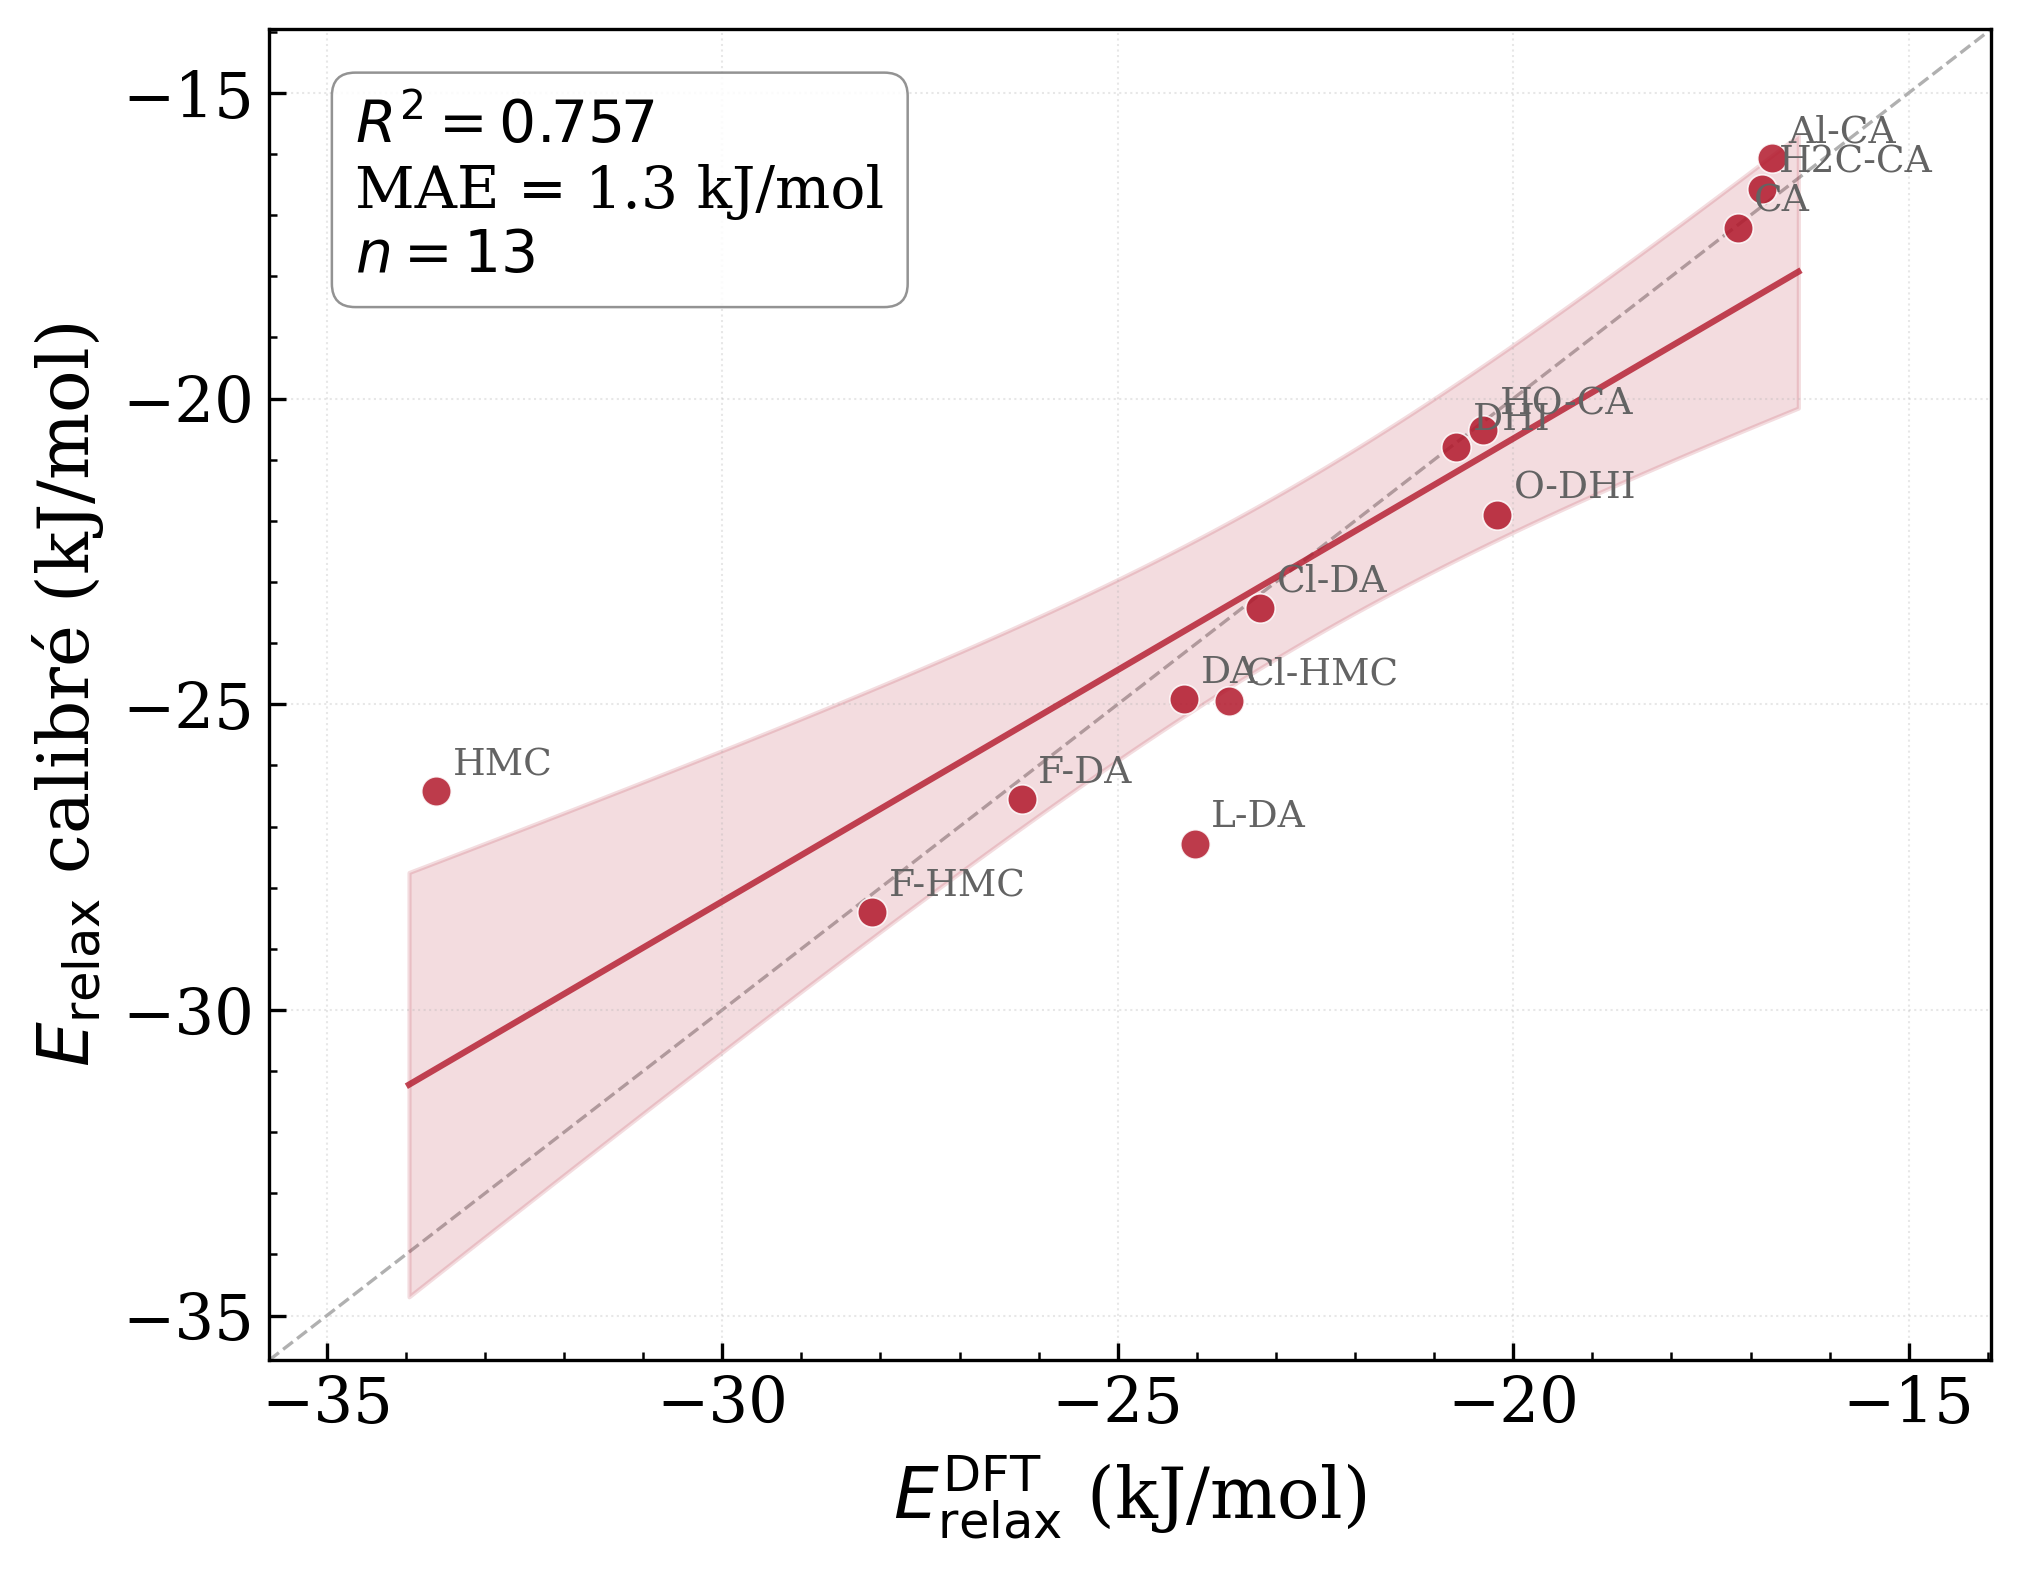
\includegraphics[width=\textwidth]{fmaxO_noparam_ox.png}
\caption{Oxydation --- $f^-_{\max,\text{O}}$.}
\label{fig:fmaxO_np_ox}
\end{subfigure}
\hfill
\begin{subfigure}[t]{0.42\textwidth}
\centering
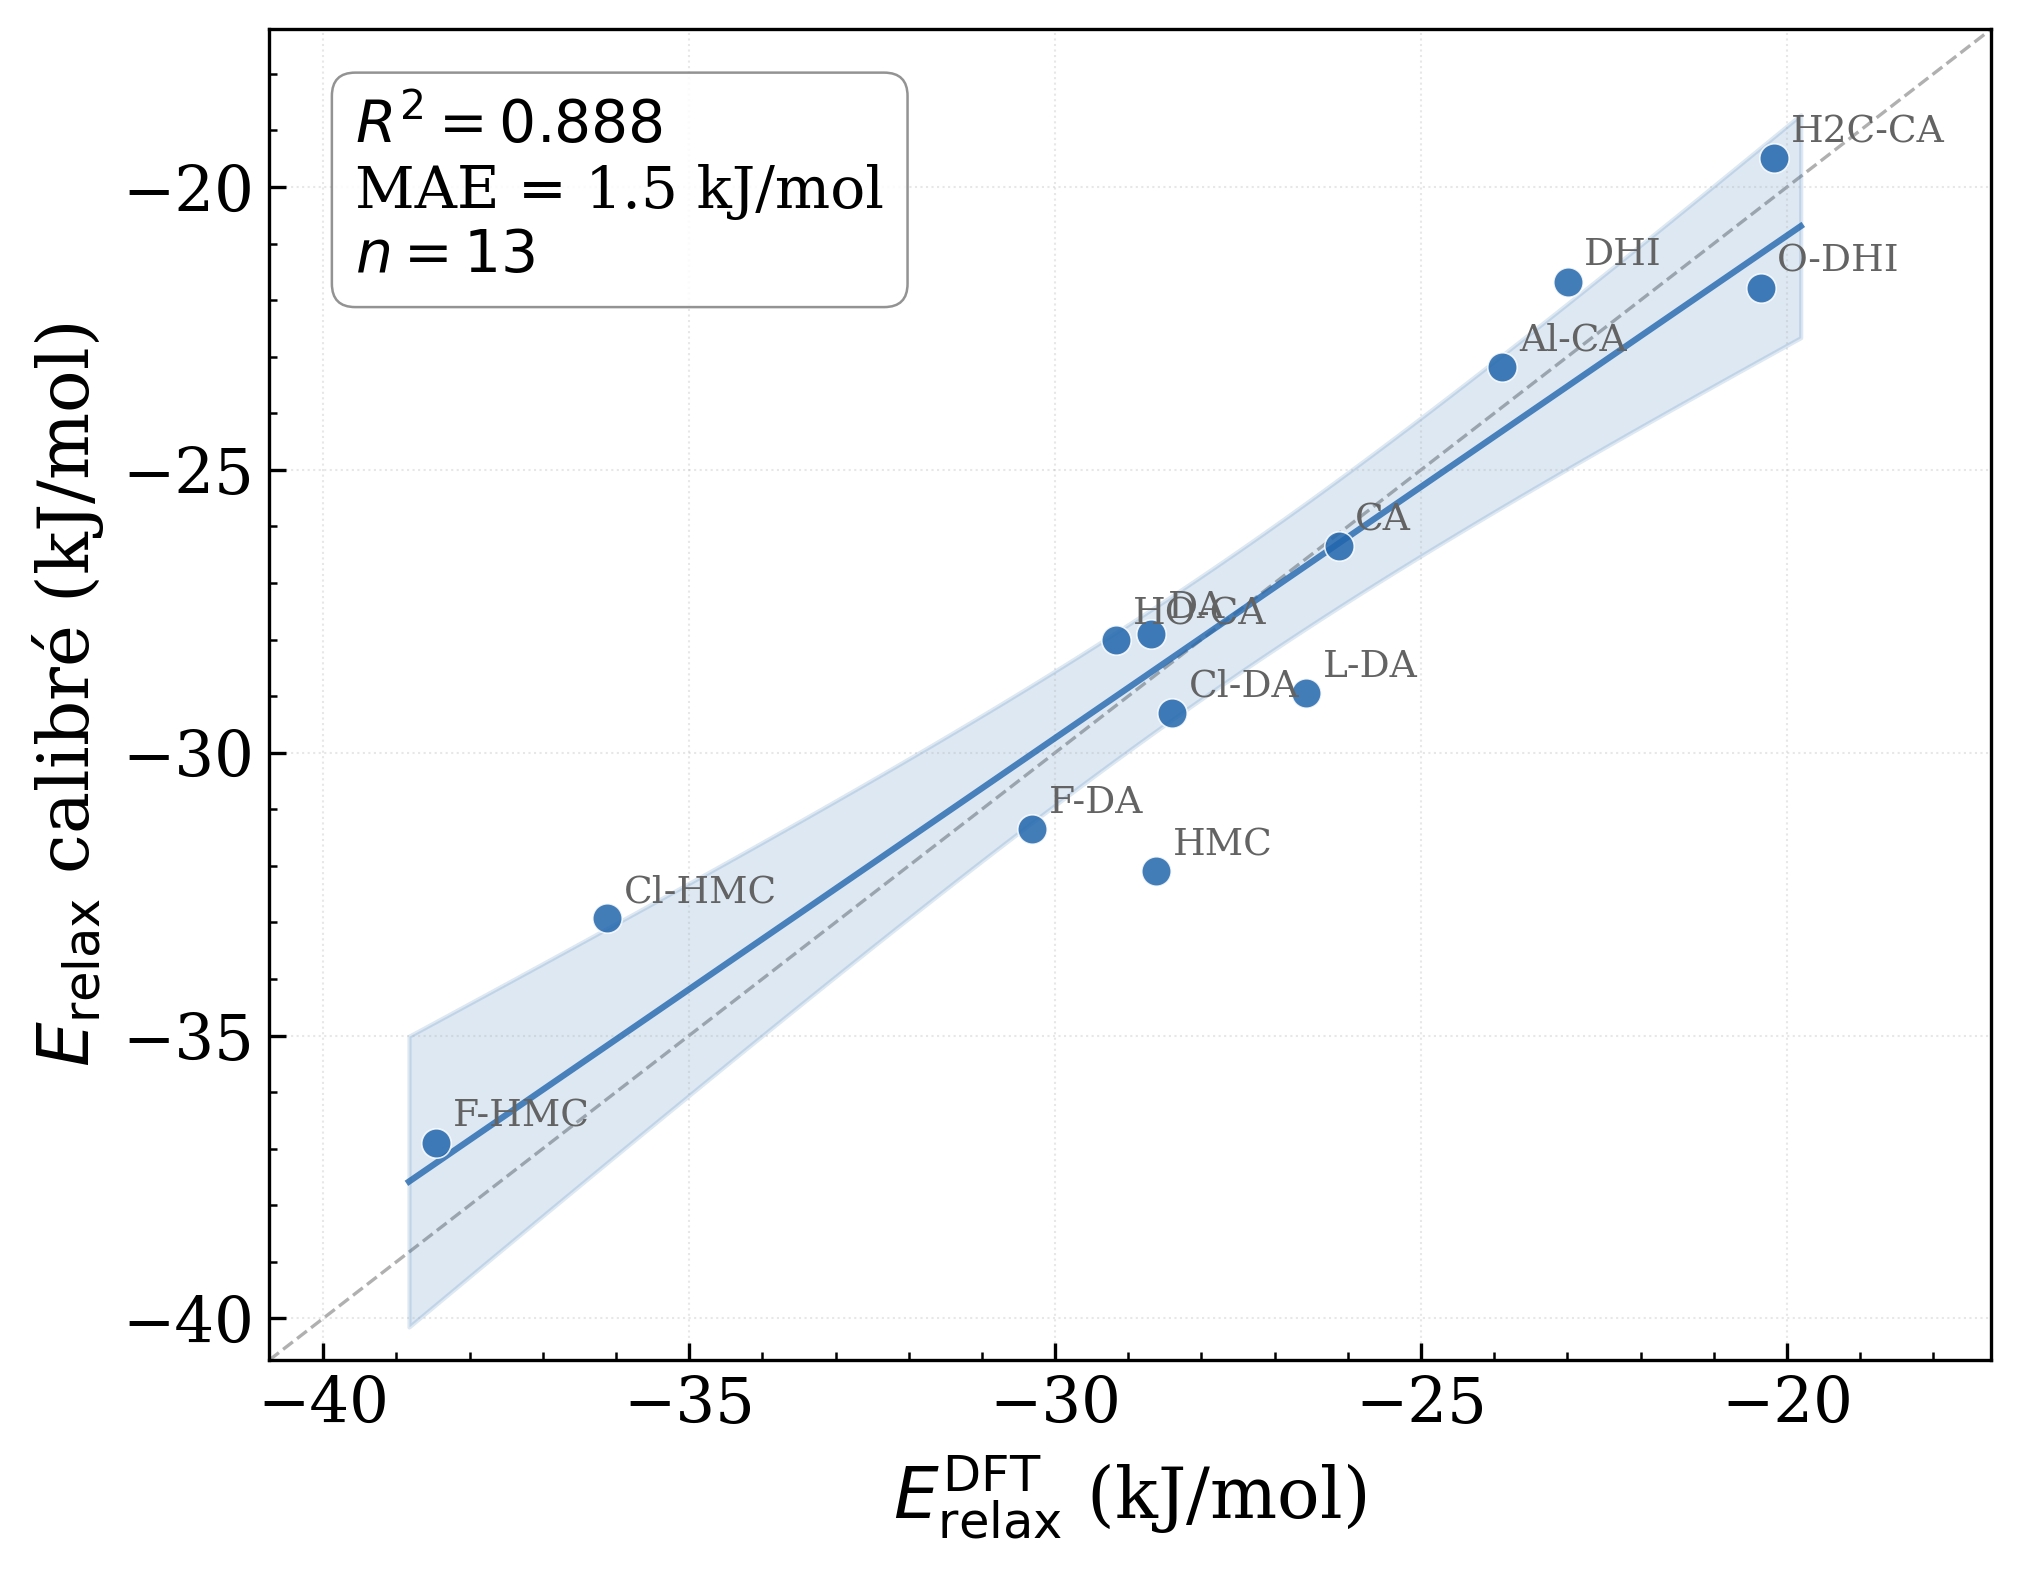
\includegraphics[width=\textwidth]{fmaxO_noparam_red.png}
\caption{Réduction --- $f^+_{\max,\text{O}}$.}
\label{fig:fmaxO_np_red}
\end{subfigure}
\caption{Modèle symétrique $f^{\pm}_{\max,\text{O}}$ sans paramètre libre (éq.~\ref{eq:fmaxO_noparam}). Parity plots calibrés, $n = 13$.}
\label{fig:fmaxO_noparam}
\end{figure}

Le modèle à un paramètre libre $a$ (ajusté indépendamment par processus) :
\begin{equation}
E_{\text{relax}}^{\text{corr}} = E_{\text{relax}}^{\text{LVC2}} \times \left(1 + a\left|f^{\pm}_{\max,\text{O}}\right|^{2}\right)
\label{eq:fmaxO_param}
\end{equation}
améliore les deux processus simultanément : MAE de \SI{1.2}{kJ/mol} en oxydation ($R^2 = 0.76$, $a_{\text{ox}} = 2.6$) et \SI{1.2}{kJ/mol} en réduction ($R^2 = 0.90$, $a_{\text{red}} = 3.7$, figure~\ref{fig:fmaxO_param}). La proximité des coefficients $a$ entre les deux processus ($2.6$ vs $3.7$) renforce la cohérence physique du modèle.

\begin{figure}[H]
\centering
\begin{subfigure}[t]{0.42\textwidth}
\centering
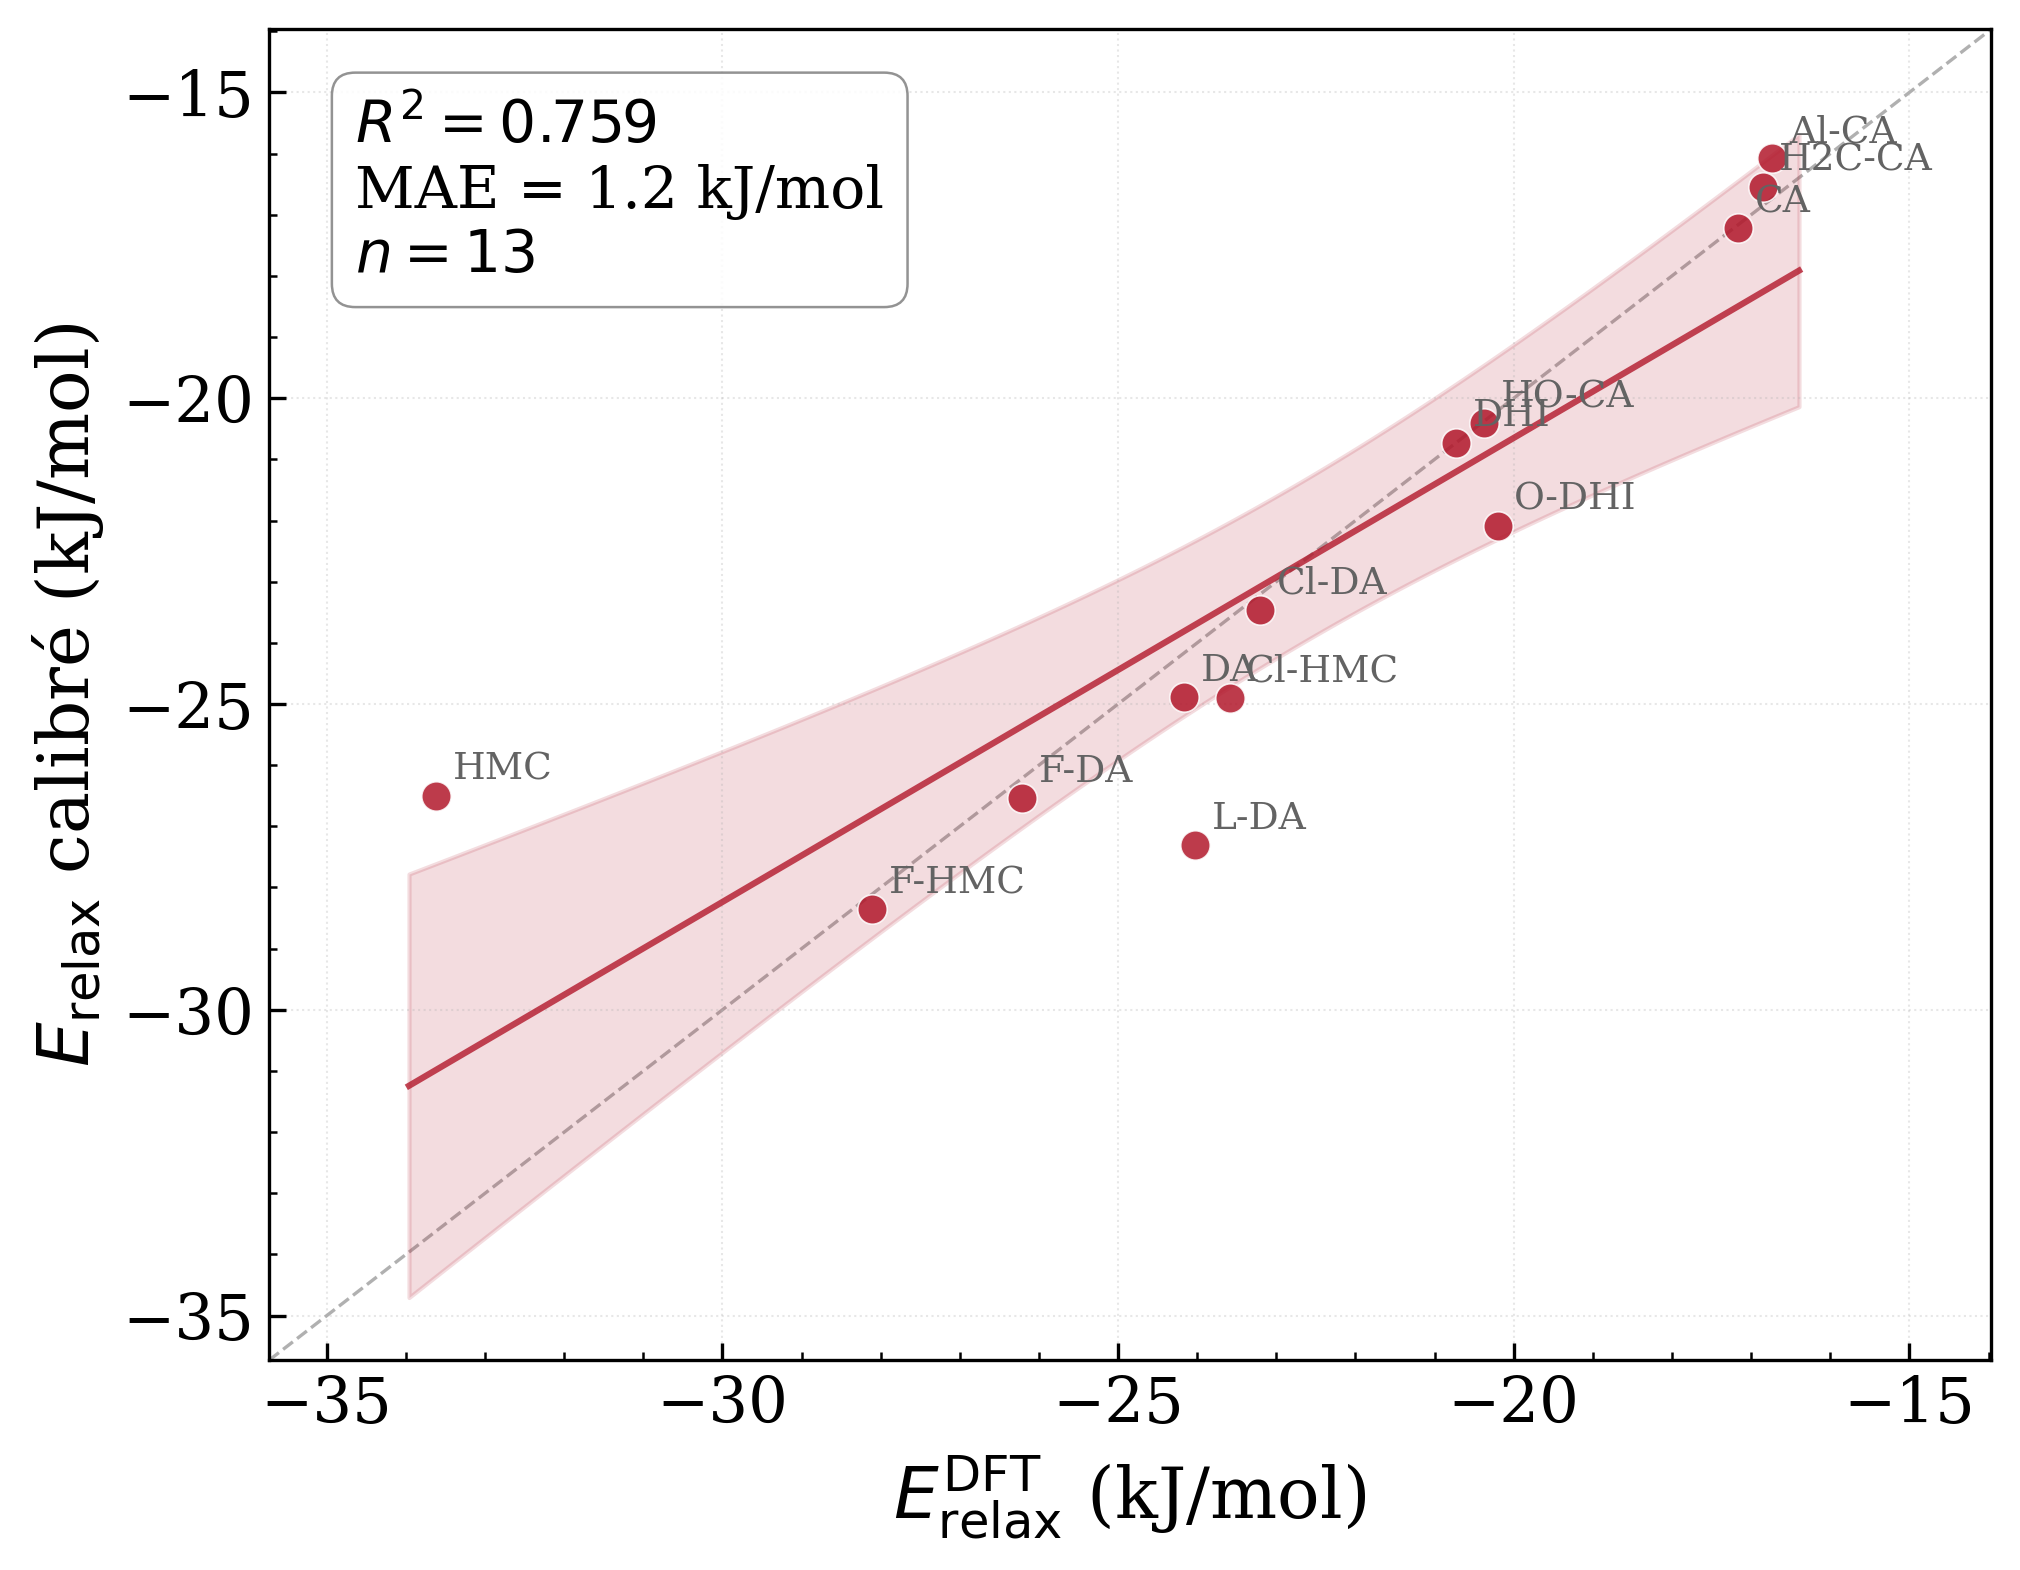
\includegraphics[width=\textwidth]{fmaxO_param_ox.png}
\caption{Oxydation ($a = 2.6$).}
\label{fig:fmaxO_p_ox}
\end{subfigure}
\hfill
\begin{subfigure}[t]{0.42\textwidth}
\centering
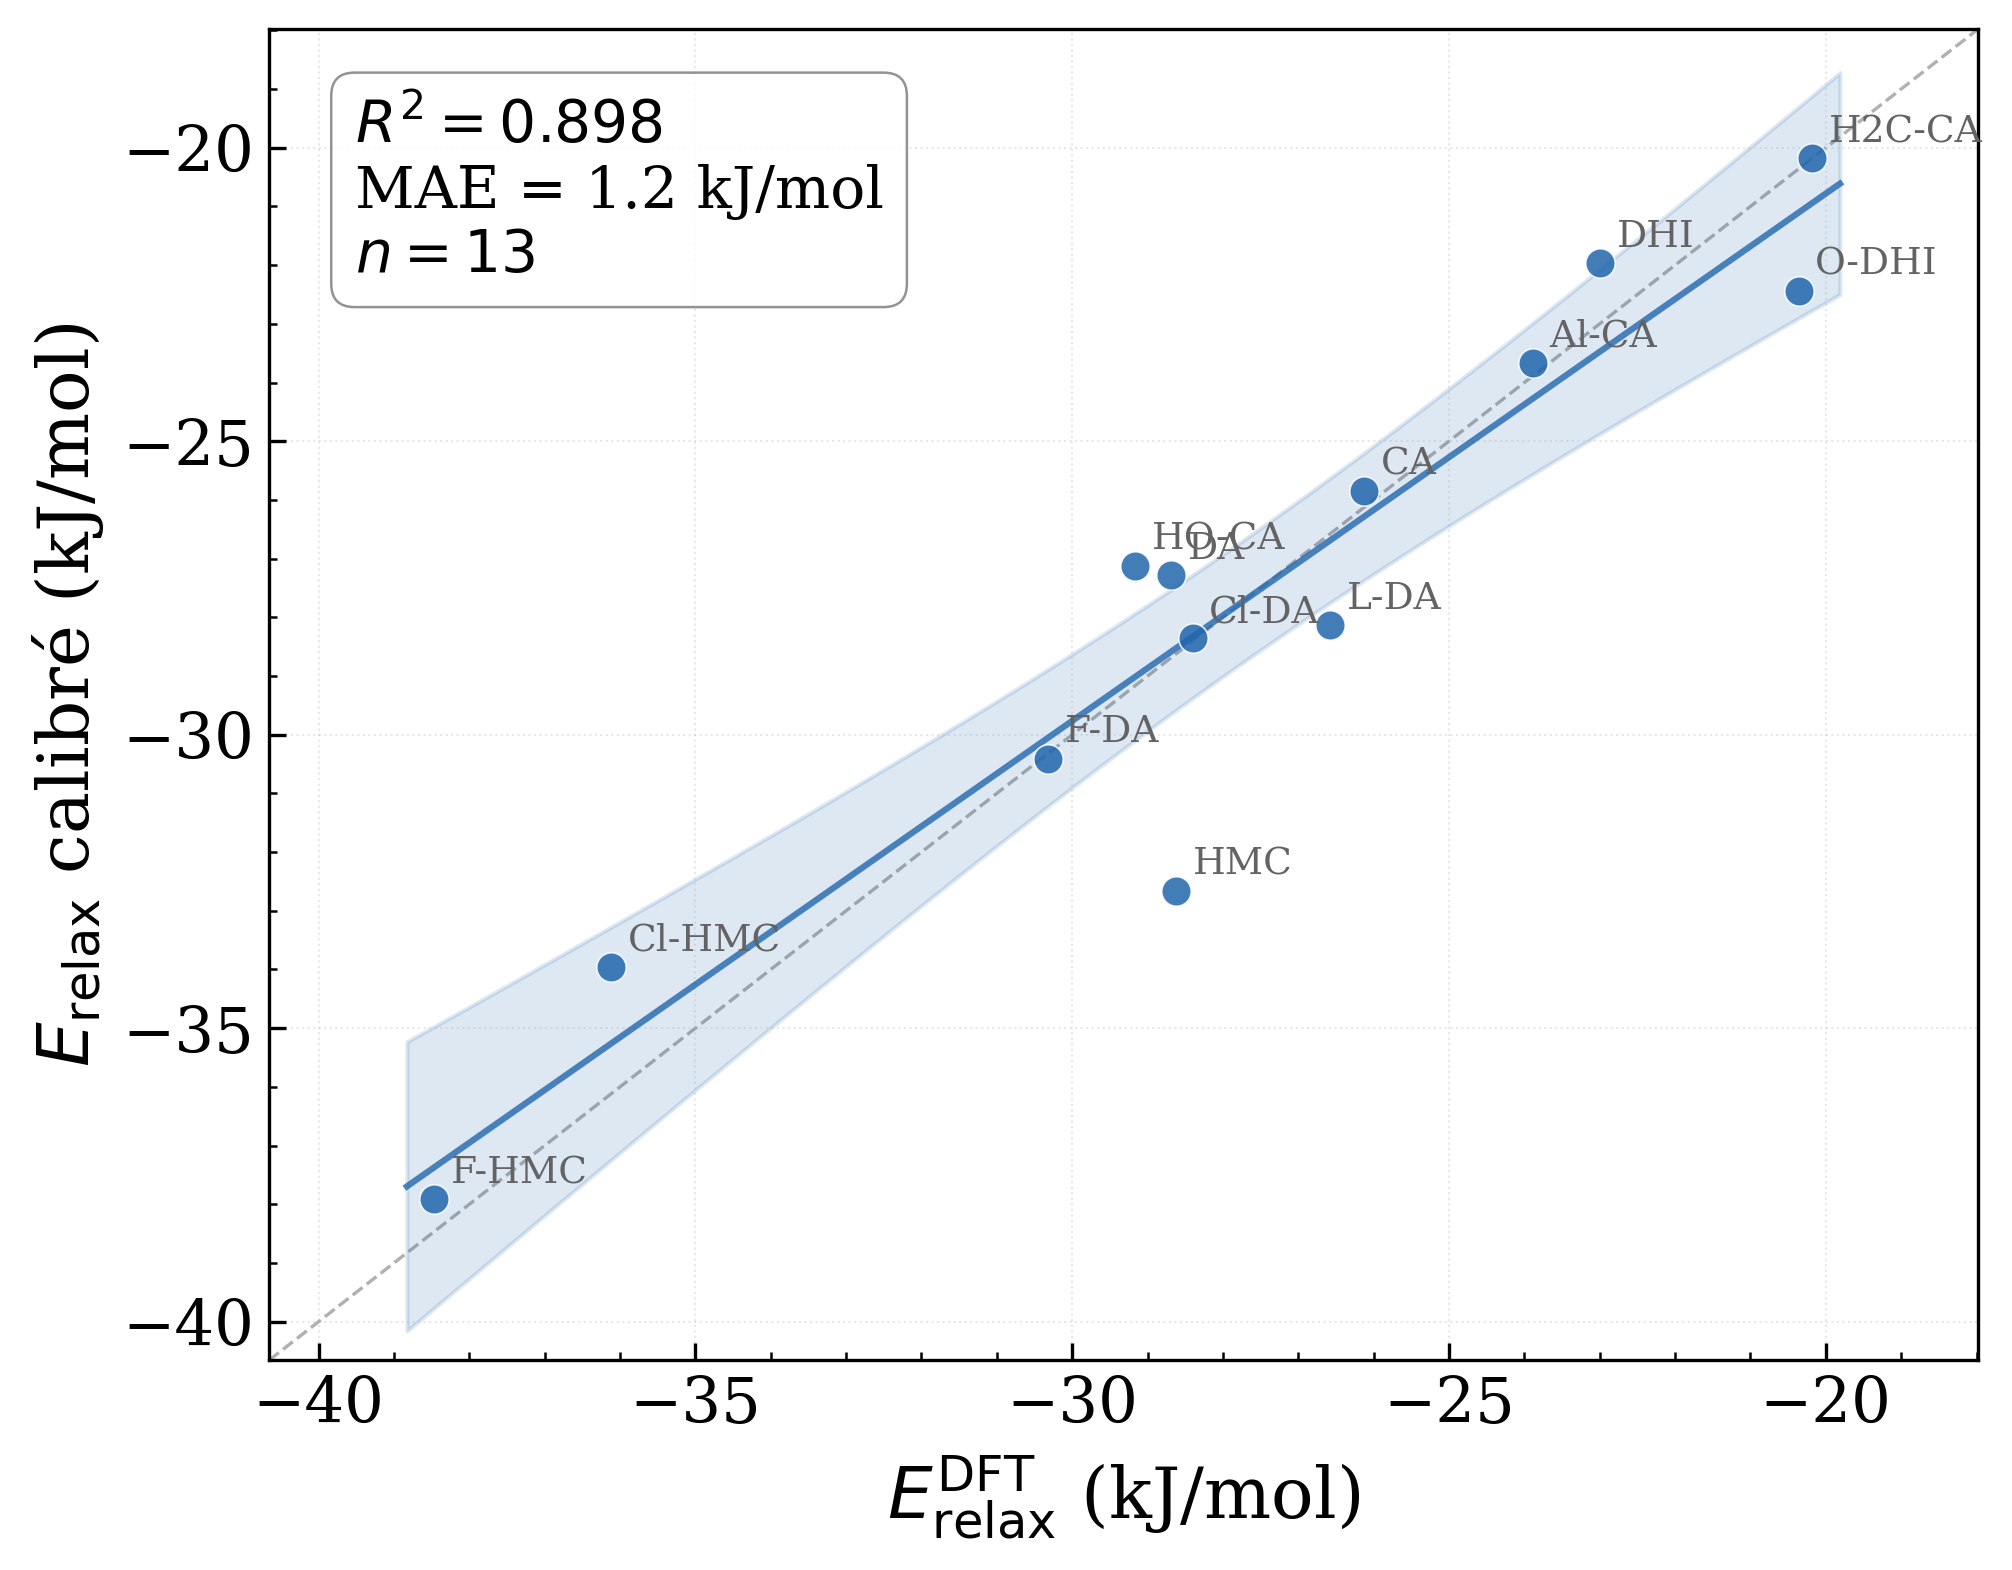
\includegraphics[width=\textwidth]{fmaxO_param_red.png}
\caption{Réduction ($a = 3.7$).}
\label{fig:fmaxO_p_red}
\end{subfigure}
\caption{Modèle symétrique $f^{\pm}_{\max,\text{O}}$ paramétrisé (éq.~\ref{eq:fmaxO_param}). Parity plots calibrés, $n = 13$.}
\label{fig:fmaxO_param}
\end{figure}

\paragraph{Discussion.}
Le modèle symétrique $f^{\pm}_{\max,\text{O}}$ présente un avantage conceptuel sur la correction LUMO (éq.~\ref{eq:lvc2_corr}) : il s'applique de manière cohérente aux deux processus redox en utilisant la fonction de Fukui physiquement pertinente ($f^+$ pour la réduction, $f^-$ pour l'oxydation). La quasi-identité des performances entre $f^+_{\text{sumO}}$ et $f_{\text{O}}^{\text{LUMO}}$ (figure~\ref{fig:fukui_vs_lumo}, $r = 0.98$) confirme que ces approches encodent la même physique : la participation des oxygènes du cycle catéchol au transfert d'électron. L'anharmonicité non captée par le LVC2 provient du réarrangement géométrique autour des liaisons C--O et O--H, d'autant plus important que la densité de Fukui sur l'oxygène le plus réactif est grande.

Le tableau~\ref{tab:fukui_exhaustive} (annexe~\ref{app:fukui}) récapitule l'ensemble des descripteurs testés, confirmant que seuls les descripteurs localisés sur les oxygènes portent un signal significatif.

\paragraph{Bilan quantitatif.}
Le tableau~\ref{tab:erelax_summary} récapitule les performances des modèles de prédiction de $E_{\text{relax}}$.

\begin{table}[H]
\centering
\caption{Performances des modèles de prédiction de $E_{\text{relax}}$ (MAE calibrée, kJ/mol).}
\label{tab:erelax_summary}
\footnotesize
\begin{tabular}{lcccc}
\toprule
Modèle & \#param & MAE ox & MAE red & $n$ \\
\midrule
LVC2 brut & 0 & 1.3 & 1.7 & 13--15 \\
LVC2 $\times (1 + (f_{\text{O}}^{\text{LUMO}})^2)$ & 0 & 1.5 & 1.4 & 15 \\
LVC2 $\times (1 + |f^{\pm}_{\max,\text{O}}|^{3/2})$ & 0 & 1.3 & 1.5 & 13 \\
LVC2 $\times (1 + a|f^{\pm}_{\max,\text{O}}|^{2})$ & 1 & 1.2 & 1.2 & 13 \\
\bottomrule
\end{tabular}
\end{table}

Le budget d'erreur par composante est détaillé dans le tableau~\ref{tab:component_models} (section~\ref{sec:dG_combined}).

\subsection{Prédiction de $\Delta\Delta U$}
\label{sec:ddU}

Le terme $\Delta\Delta U = [U(\text{ion}_{\text{opt}}) - E_e(\text{ion}_{\text{opt}})] - [U(\text{neutre}) - E_e(\text{neutre})]$ capture le changement d'énergie interne thermique (dominé par la ZPE) lors du changement d'état de charge. En oxydation, $\Delta\Delta U$ est toujours positif (moyenne $\SI{0.5 \pm 0.6}{kJ/mol}$), reflétant un léger raidissement des liaisons C--O. En réduction, il est toujours négatif (moyenne $\SI{-12.7 \pm 2.2}{kJ/mol}$), traduisant un assouplissement de la structure.

\paragraph{Échec du prédicteur ZPE.}
La ZPE de l'état neutre ne corrèle pas avec $\Delta\Delta U$ ($R^2 < 0.01$, $p > 0.7$), car $\Delta\Delta U$ dépend des \emph{différences} de fréquences entre états neutre et ionique, contrôlées par la redistribution de charge locale, et non de la ZPE absolue (liée à la taille moléculaire).

\paragraph{Descripteur : dureté chimique $\eta$.}
La dureté chimique $\eta = (\text{IP} - \text{EA})/2$ mesure la résistance de la molécule au transfert de charge. Une molécule « dure » (grand $\eta$) voit ses fréquences vibrationnelles moins perturbées par l'ajout ou le retrait d'un électron, ce qui devrait se traduire par un $|\Delta\Delta U|$ plus faible. Ce descripteur est disponible sans coût supplémentaire puisque IP et EA verticaux sont déjà calculés lors du single-point ionique.

\paragraph{Résultats.}
La figure~\ref{fig:ddU_eta} montre les corrélations $\eta$ vs $\Delta\Delta U$ pour les 15 catéchols.
\begin{itemize}[noitemsep]
\item \textbf{Réduction} : la corrélation est forte ($R^2_{\text{adj}} = 0.72$, $n = 15$). Le modèle linéaire :
\begin{equation}
\Delta\Delta U_{\text{red}} = 0.67 - 0.060\,\eta \quad \text{(kJ/mol)}
\label{eq:ddU_red_eta}
\end{equation}
donne une MAE de \SI{0.75}{kJ/mol}, soit une amélioration d'un facteur 2.3 par rapport au modèle constant (MAE $= \SI{1.7}{kJ/mol}$). La pente négative confirme l'interprétation : les molécules plus dures subissent un assouplissement vibrationnel plus faible lors de la réduction.
\item \textbf{Oxydation} : $\Delta\Delta U_{\text{ox}}$ présente une variance trop faible ($\sigma = \SI{0.6}{kJ/mol}$) pour justifier un modèle au-delà de la constante. Le modèle constant $\Delta\Delta U_{\text{ox}} \approx \SI{+0.5}{kJ/mol}$ (MAE $= \SI{0.4}{kJ/mol}$) est retenu.
\end{itemize}

\begin{figure}[H]
\centering
\begin{subfigure}[t]{0.48\textwidth}
\centering
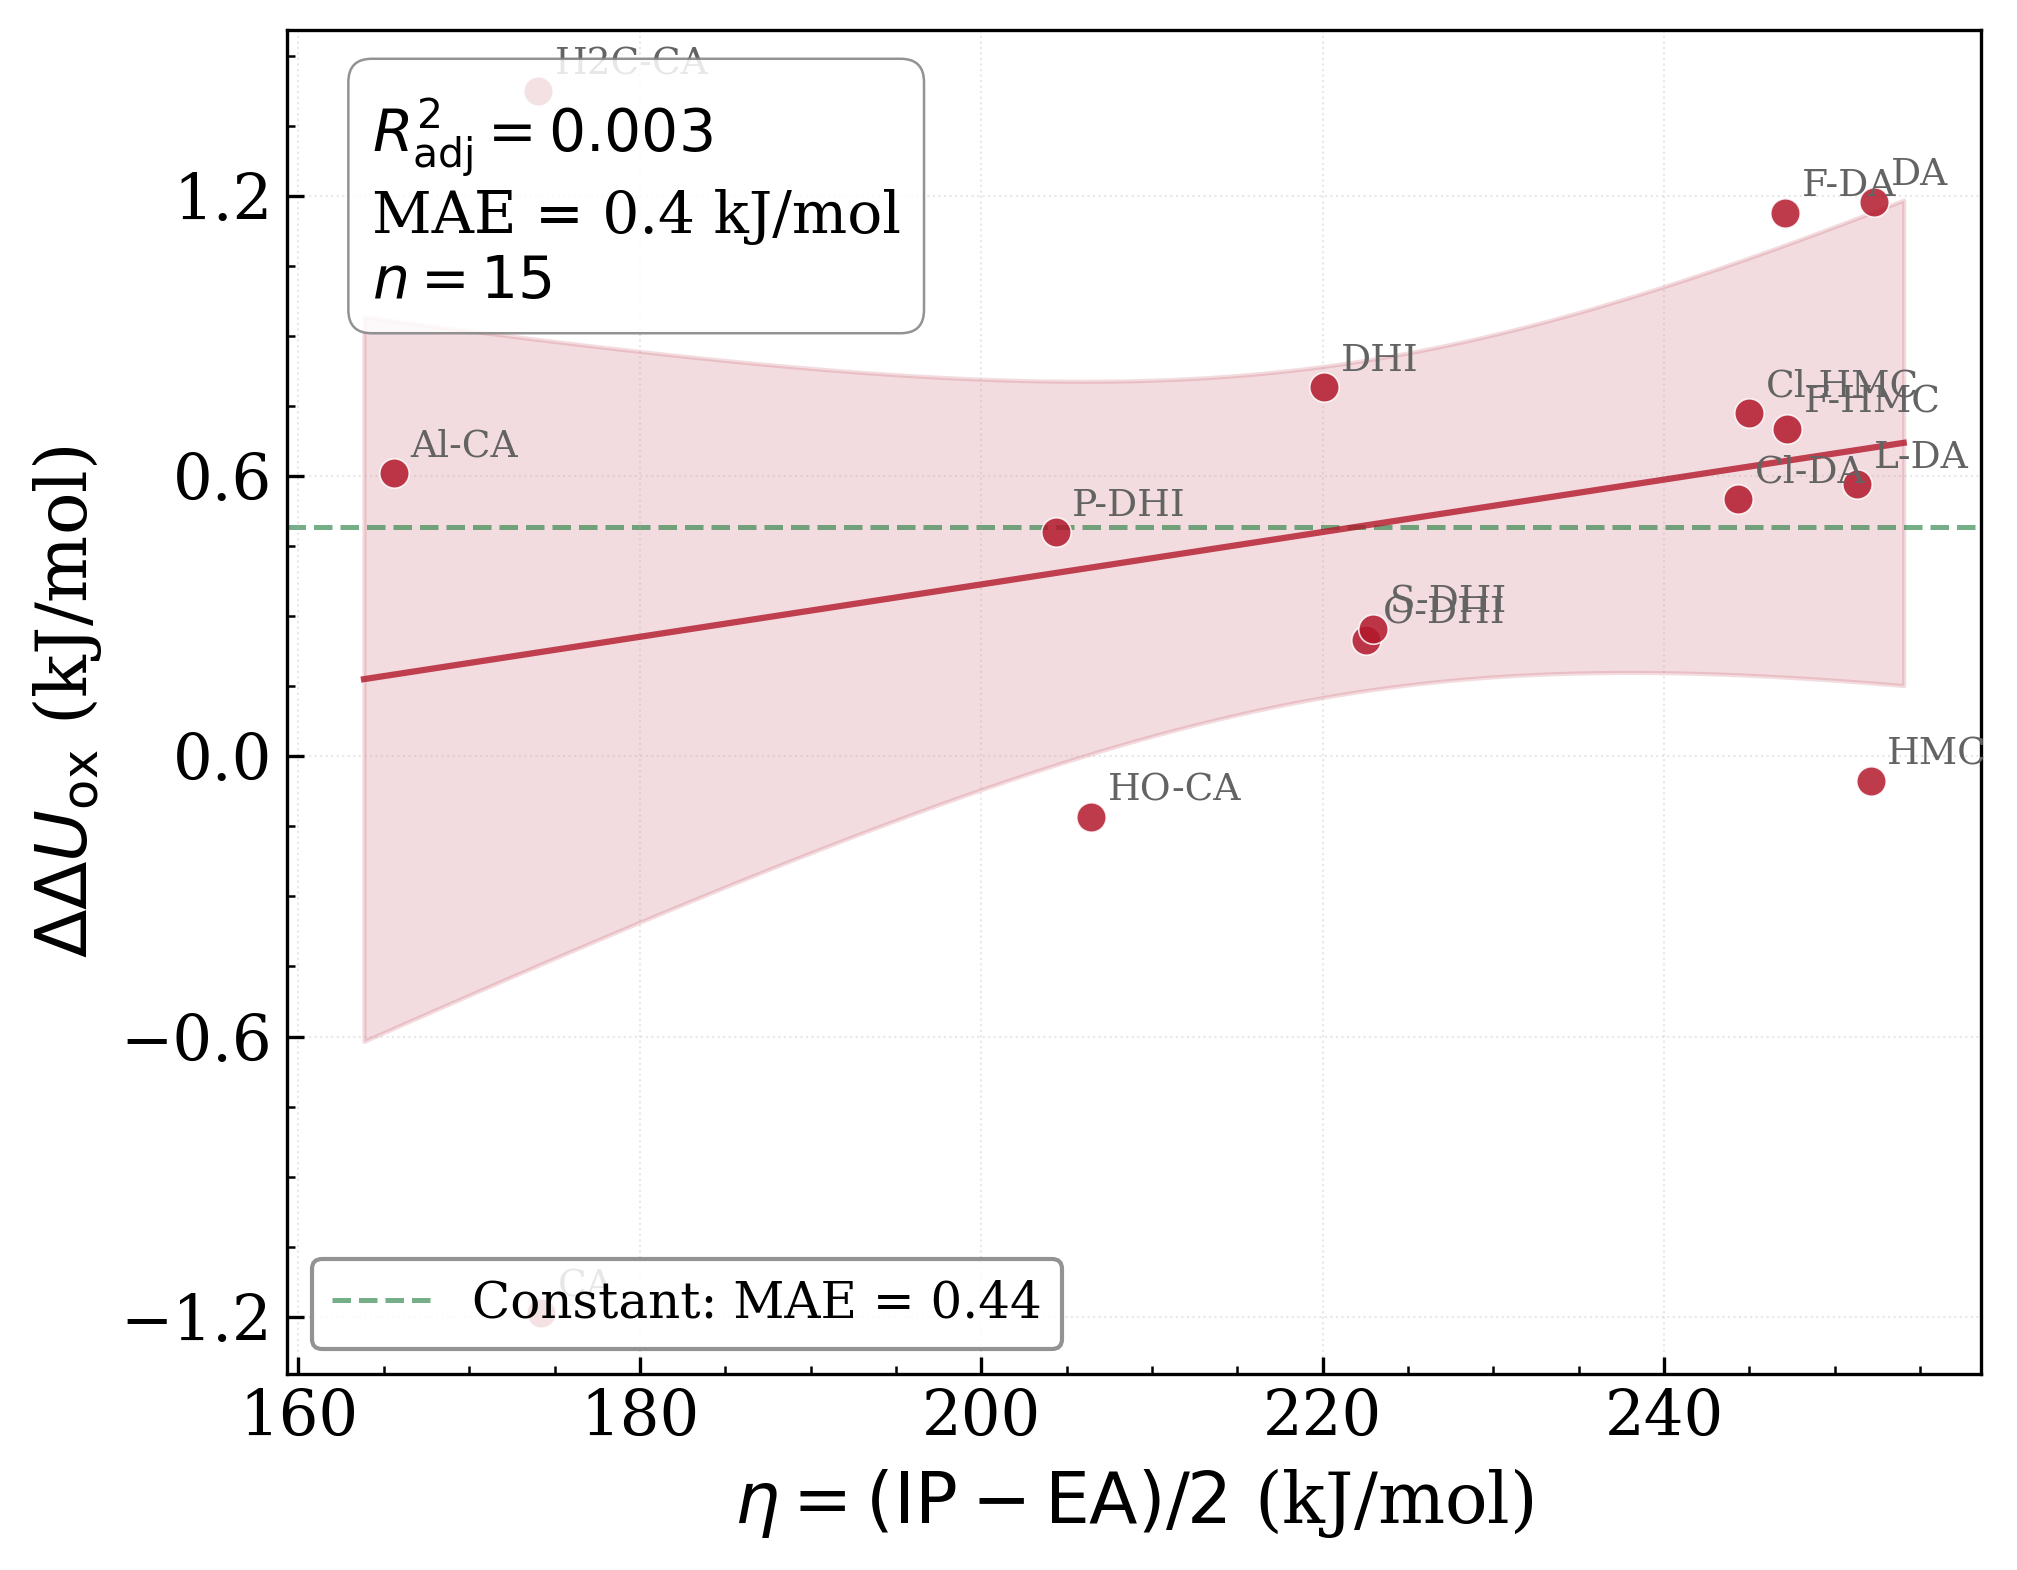
\includegraphics[width=\textwidth]{thermodynamic_models/ddU_eta_ox.png}
\caption{Oxydation.}
\label{fig:ddU_eta_ox}
\end{subfigure}
\hfill
\begin{subfigure}[t]{0.48\textwidth}
\centering
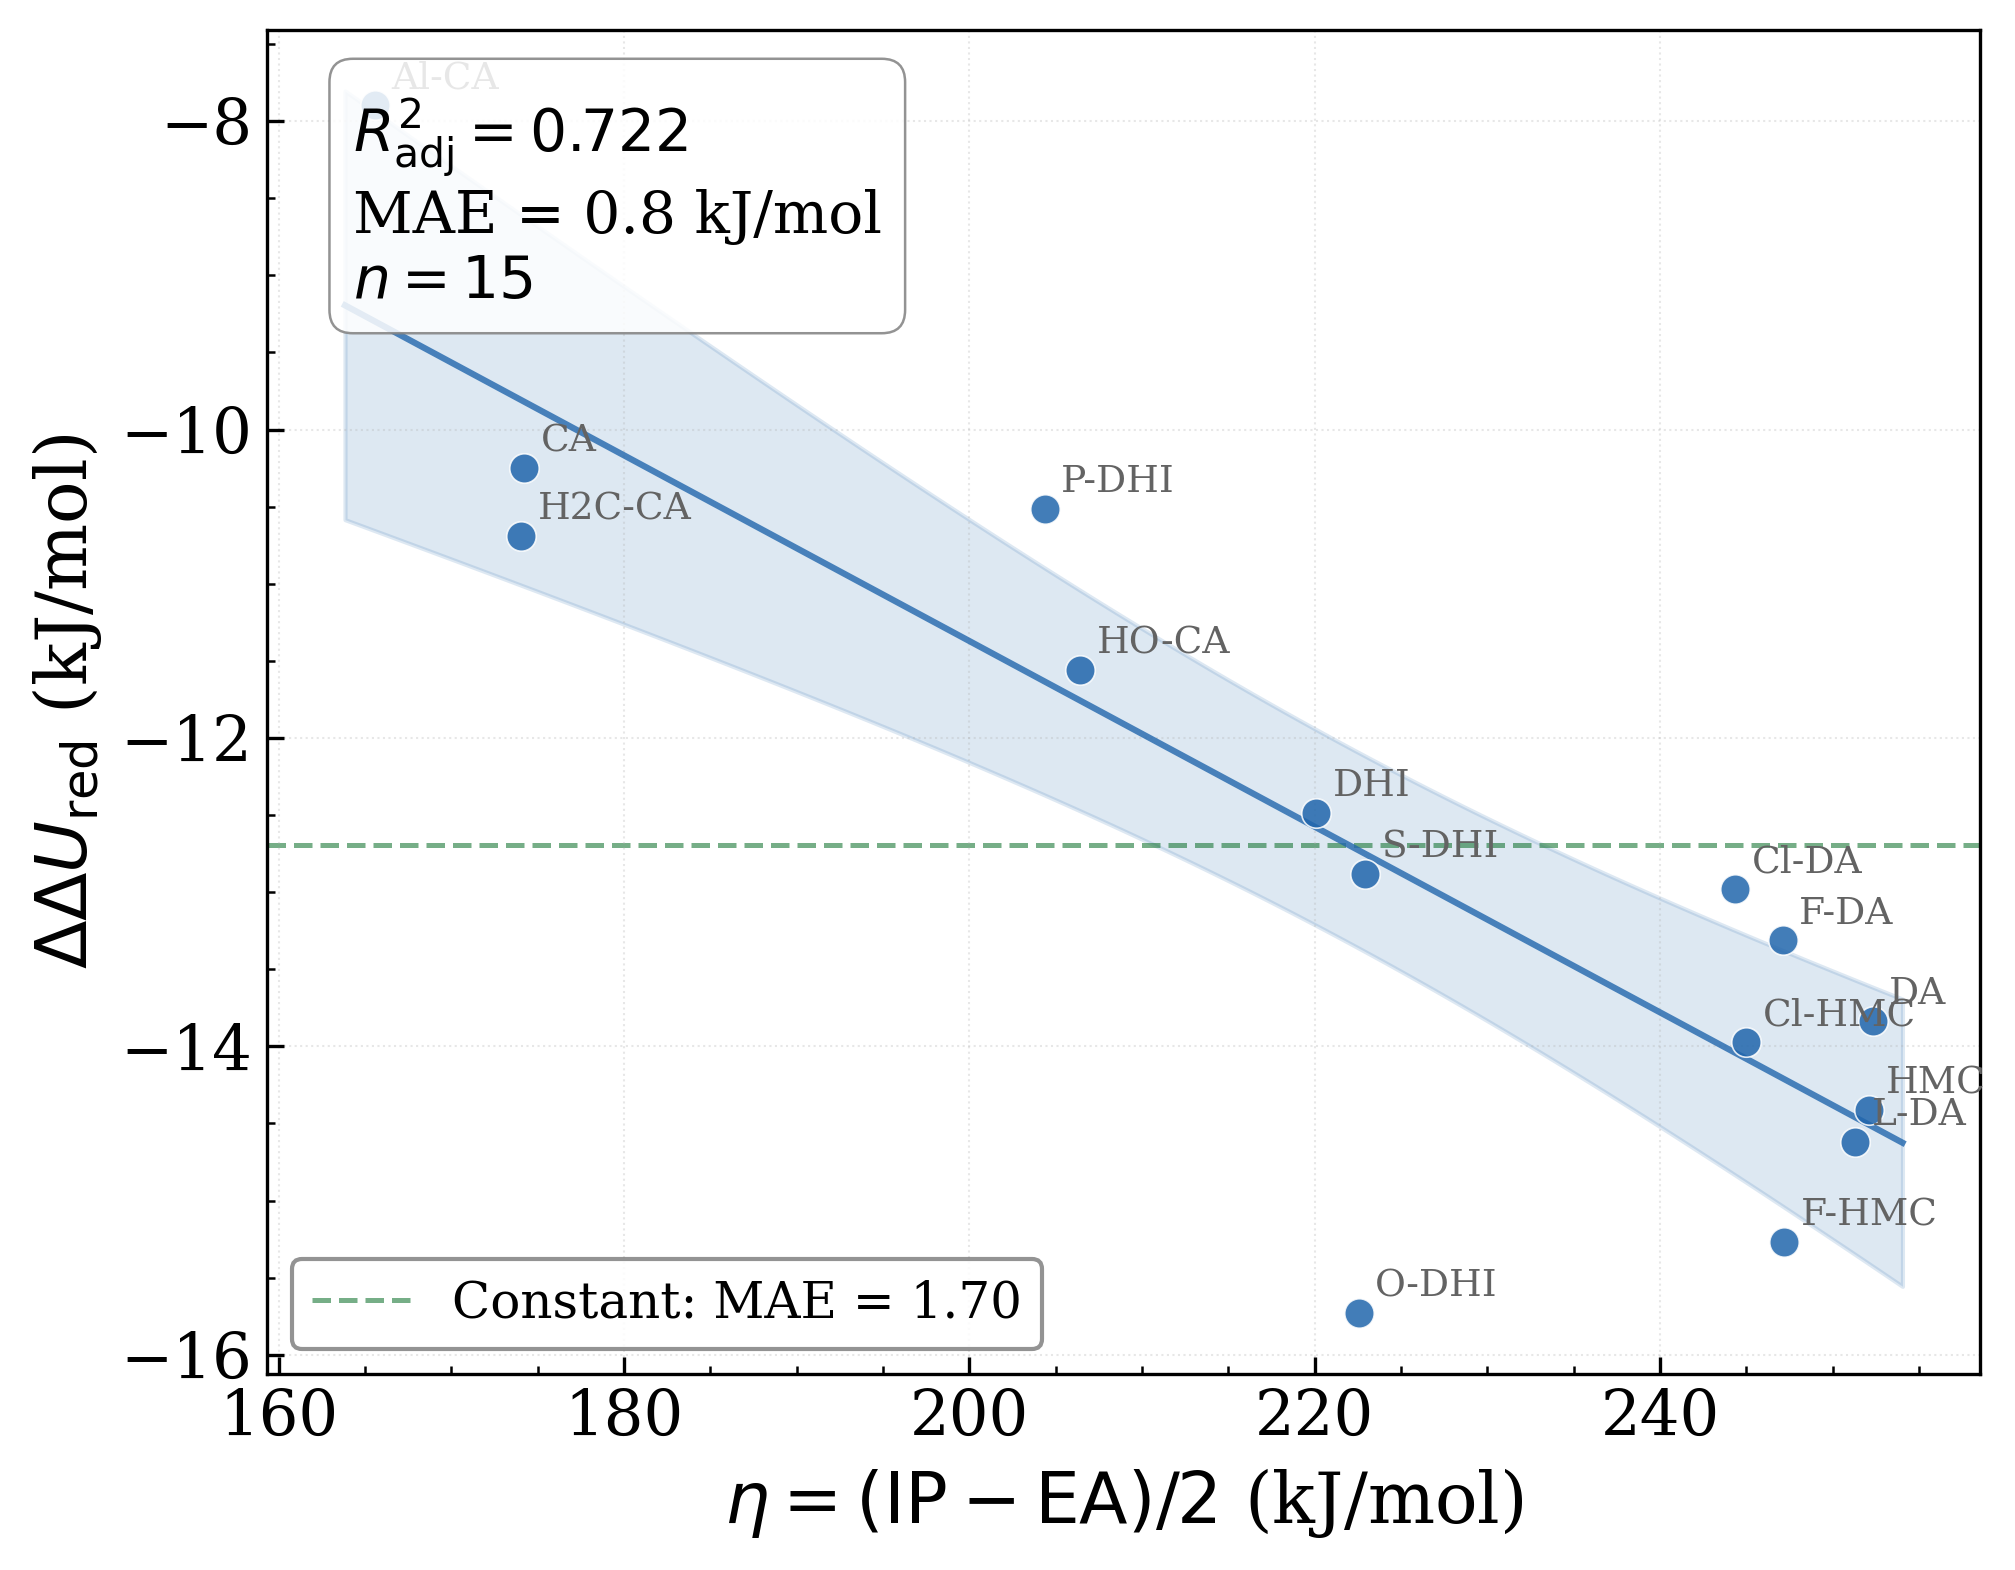
\includegraphics[width=\textwidth]{thermodynamic_models/ddU_eta_red.png}
\caption{Réduction.}
\label{fig:ddU_eta_red}
\end{subfigure}
\caption{Dureté chimique $\eta$ vs $\Delta\Delta U$ pour les 15 catéchols. Régressions linéaires (trait plein) avec bande de confiance à 95\%, et modèles constants (pointillés verts). En réduction, $\eta$ explique 72\% de la variance ($p < 10^{-4}$).}
\label{fig:ddU_eta}
\end{figure}

Une recherche exhaustive de descripteurs (indices de Fukui, descripteurs CDFT globaux, charges de Bader, indices de délocalisation QTAIM) confirme que $\eta$ est le meilleur prédicteur à un descripteur pour $\Delta\Delta U_{\text{red}}$. Des modèles à deux descripteurs, comme $(\text{DI}_{\text{sumO}}, \omega)$ avec $\omega = \mu^2/(2\eta)$ l'électrophilicité globale, atteignent une MAE de \SI{0.54}{kJ/mol} ($R^2_{\text{adj}} = 0.86$, $n = 13$), mais le gain marginal ne justifie pas la complexité supplémentaire ni la perte de 2 molécules.

%-----------------------------------------------------------------------
\subsection{Prédiction de $T\Delta S$}
\label{sec:TdS}

Le terme entropique $T\Delta S = T[S(\text{ion}_{\text{opt}}) - S(\text{neutre})]$ est dominé par l'entropie vibrationnelle. En oxydation, $T\Delta S$ est quasi-systématiquement négatif (moyenne $\SI{-2.6 \pm 1.1}{kJ/mol}$), cohérent avec le raidissement des liaisons lors du passage catéchol~$\to$~quinone. En réduction, il est positif (moyenne $\SI{2.6 \pm 2.5}{kJ/mol}$), reflétant un assouplissement structural.

\paragraph{Descripteur initial : entropie vibrationnelle RRHO.}
L'entropie vibrationnelle de l'état neutre est calculée dans l'approximation RRHO (Rigid Rotor--Harmonic Oscillator) :
\begin{equation}
S_{\text{vib}} = R \sum_k \left[ \frac{u_k}{e^{u_k} - 1} - \ln\left(1 - e^{-u_k}\right) \right]
\label{eq:svib}
\end{equation}
où $u_k = \hbar\omega_k / (k_BT)$ et la somme porte sur tous les modes normaux de fréquence $\omega_k > \SI{10}{cm^{-1}}$. Les valeurs de $TS_{\text{vib}}$ s'échelonnent de \SIrange{25}{47}{kJ/mol}. La corrélation $TS_{\text{vib}}$ vs $T\Delta S$ est faible en réduction ($R^2 = 0.23$, $p = 0.070$) et inexistante en oxydation ($R^2 = 0.06$, $p = 0.38$). $TS_{\text{vib}}$ mesure l'entropie \emph{absolue}, alors que $T\Delta S$ dépend de la façon dont les modes vibrationnels \emph{changent} lors de l'ionisation.

\paragraph{Descripteurs QTAIM : charge de Bader et potentiel chimique.}
Une recherche exhaustive de descripteurs issus de la DFT conceptuelle et de l'analyse QTAIM identifie la paire $(\text{bader}_{\text{sumO}}, \mu)$ comme meilleur prédicteur de $T\Delta S$. La charge de Bader totale sur les atomes d'oxygène ($\text{bader}_{\text{sumO}}$) reflète le degré d'ionicité des liaisons C--O, qui module les fréquences basse énergie (torsions, vibrations hors du plan) dont l'entropie vibrationnelle dépend. Le potentiel chimique $\mu = -(\text{IP} + \text{EA})/2$ complète ce descripteur en capturant la tendance globale au transfert de charge.

\paragraph{Résultats.}
Le modèle bilinéaire :
\begin{align}
T\Delta S_{\text{red}} &= 1.05\,\text{bader}_{\text{sumO}} + 0.036\,\mu + 15.3 & \text{(kJ/mol)} \label{eq:tds_red_bader} \\
T\Delta S_{\text{ox}} &= 0.68\,\text{bader}_{\text{sumO}} - 0.005\,\mu - 4.1 & \text{(kJ/mol)} \label{eq:tds_ox_bader}
\end{align}
donne les performances suivantes ($n = 13$ molécules avec descripteurs QTAIM) :
\begin{itemize}[noitemsep]
\item \textbf{Réduction} : MAE $= \SI{1.13}{kJ/mol}$ ($R^2_{\text{adj}} = 0.33$), contre MAE $= \SI{1.76}{kJ/mol}$ pour le modèle constant --- amélioration de 36\%.
\item \textbf{Oxydation} : MAE $= \SI{0.75}{kJ/mol}$ ($R^2_{\text{adj}} = 0.04$), contre MAE $= \SI{0.87}{kJ/mol}$ pour le modèle constant --- amélioration modeste de 14\%.
\end{itemize}

La figure~\ref{fig:tds_bader} montre les parity plots pour les deux processus.

\begin{figure}[H]
\centering
\begin{subfigure}[t]{0.48\textwidth}
\centering
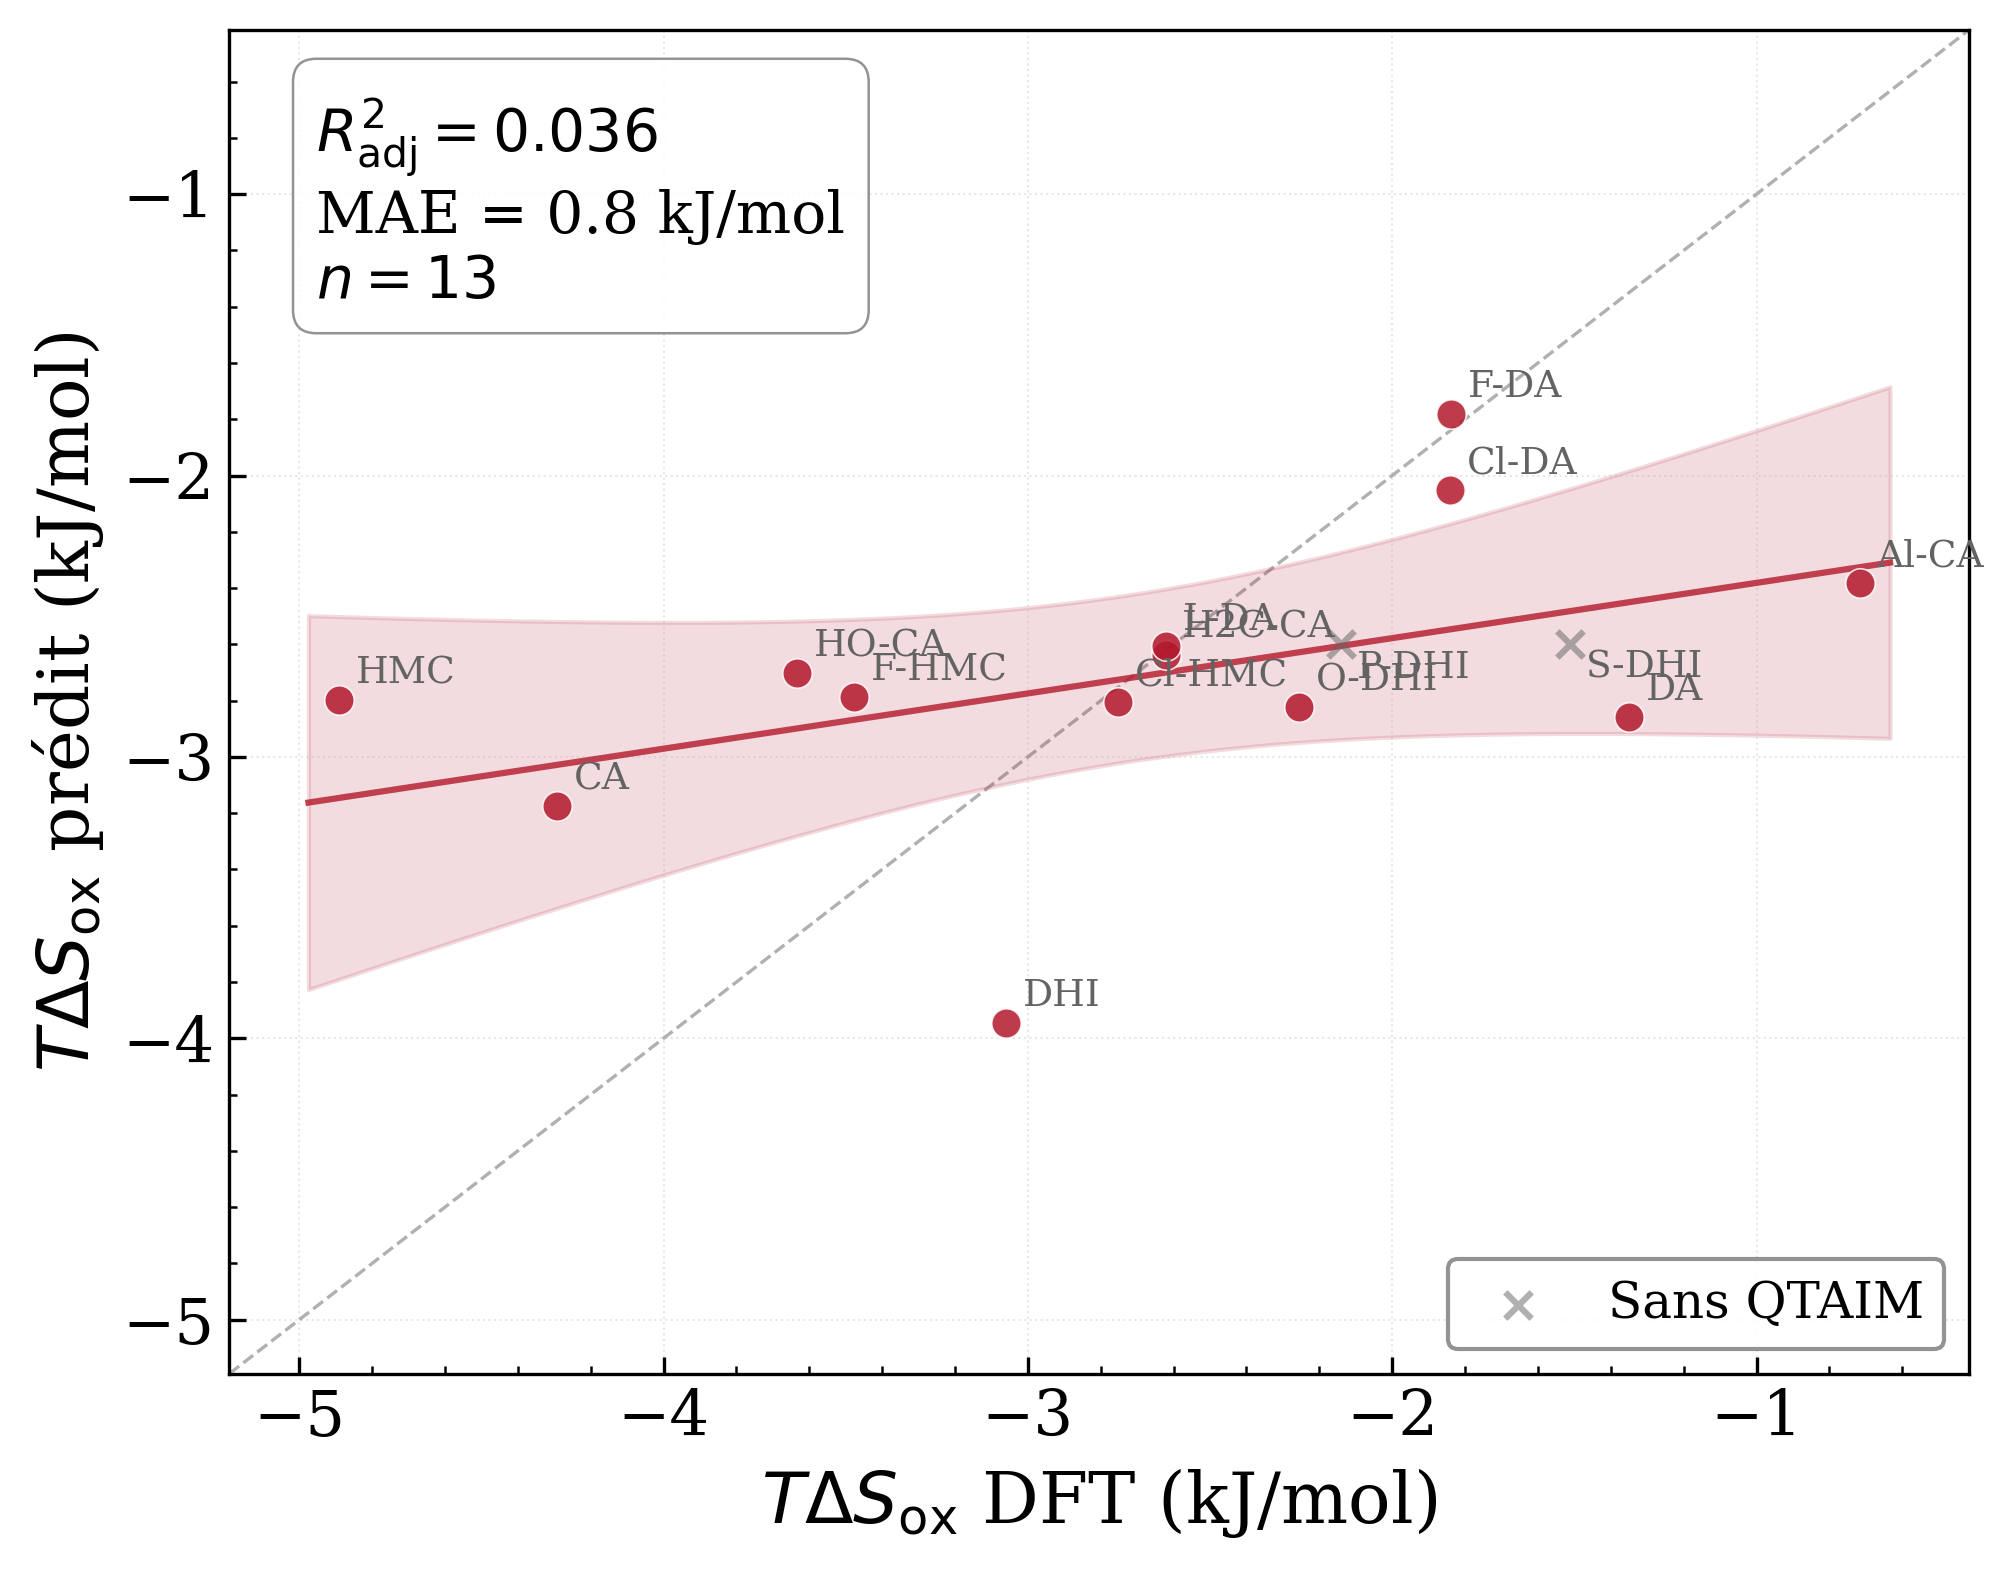
\includegraphics[width=\textwidth]{thermodynamic_models/TdS_bader_mu_ox.png}
\caption{Oxydation.}
\label{fig:tds_bader_ox}
\end{subfigure}
\hfill
\begin{subfigure}[t]{0.48\textwidth}
\centering
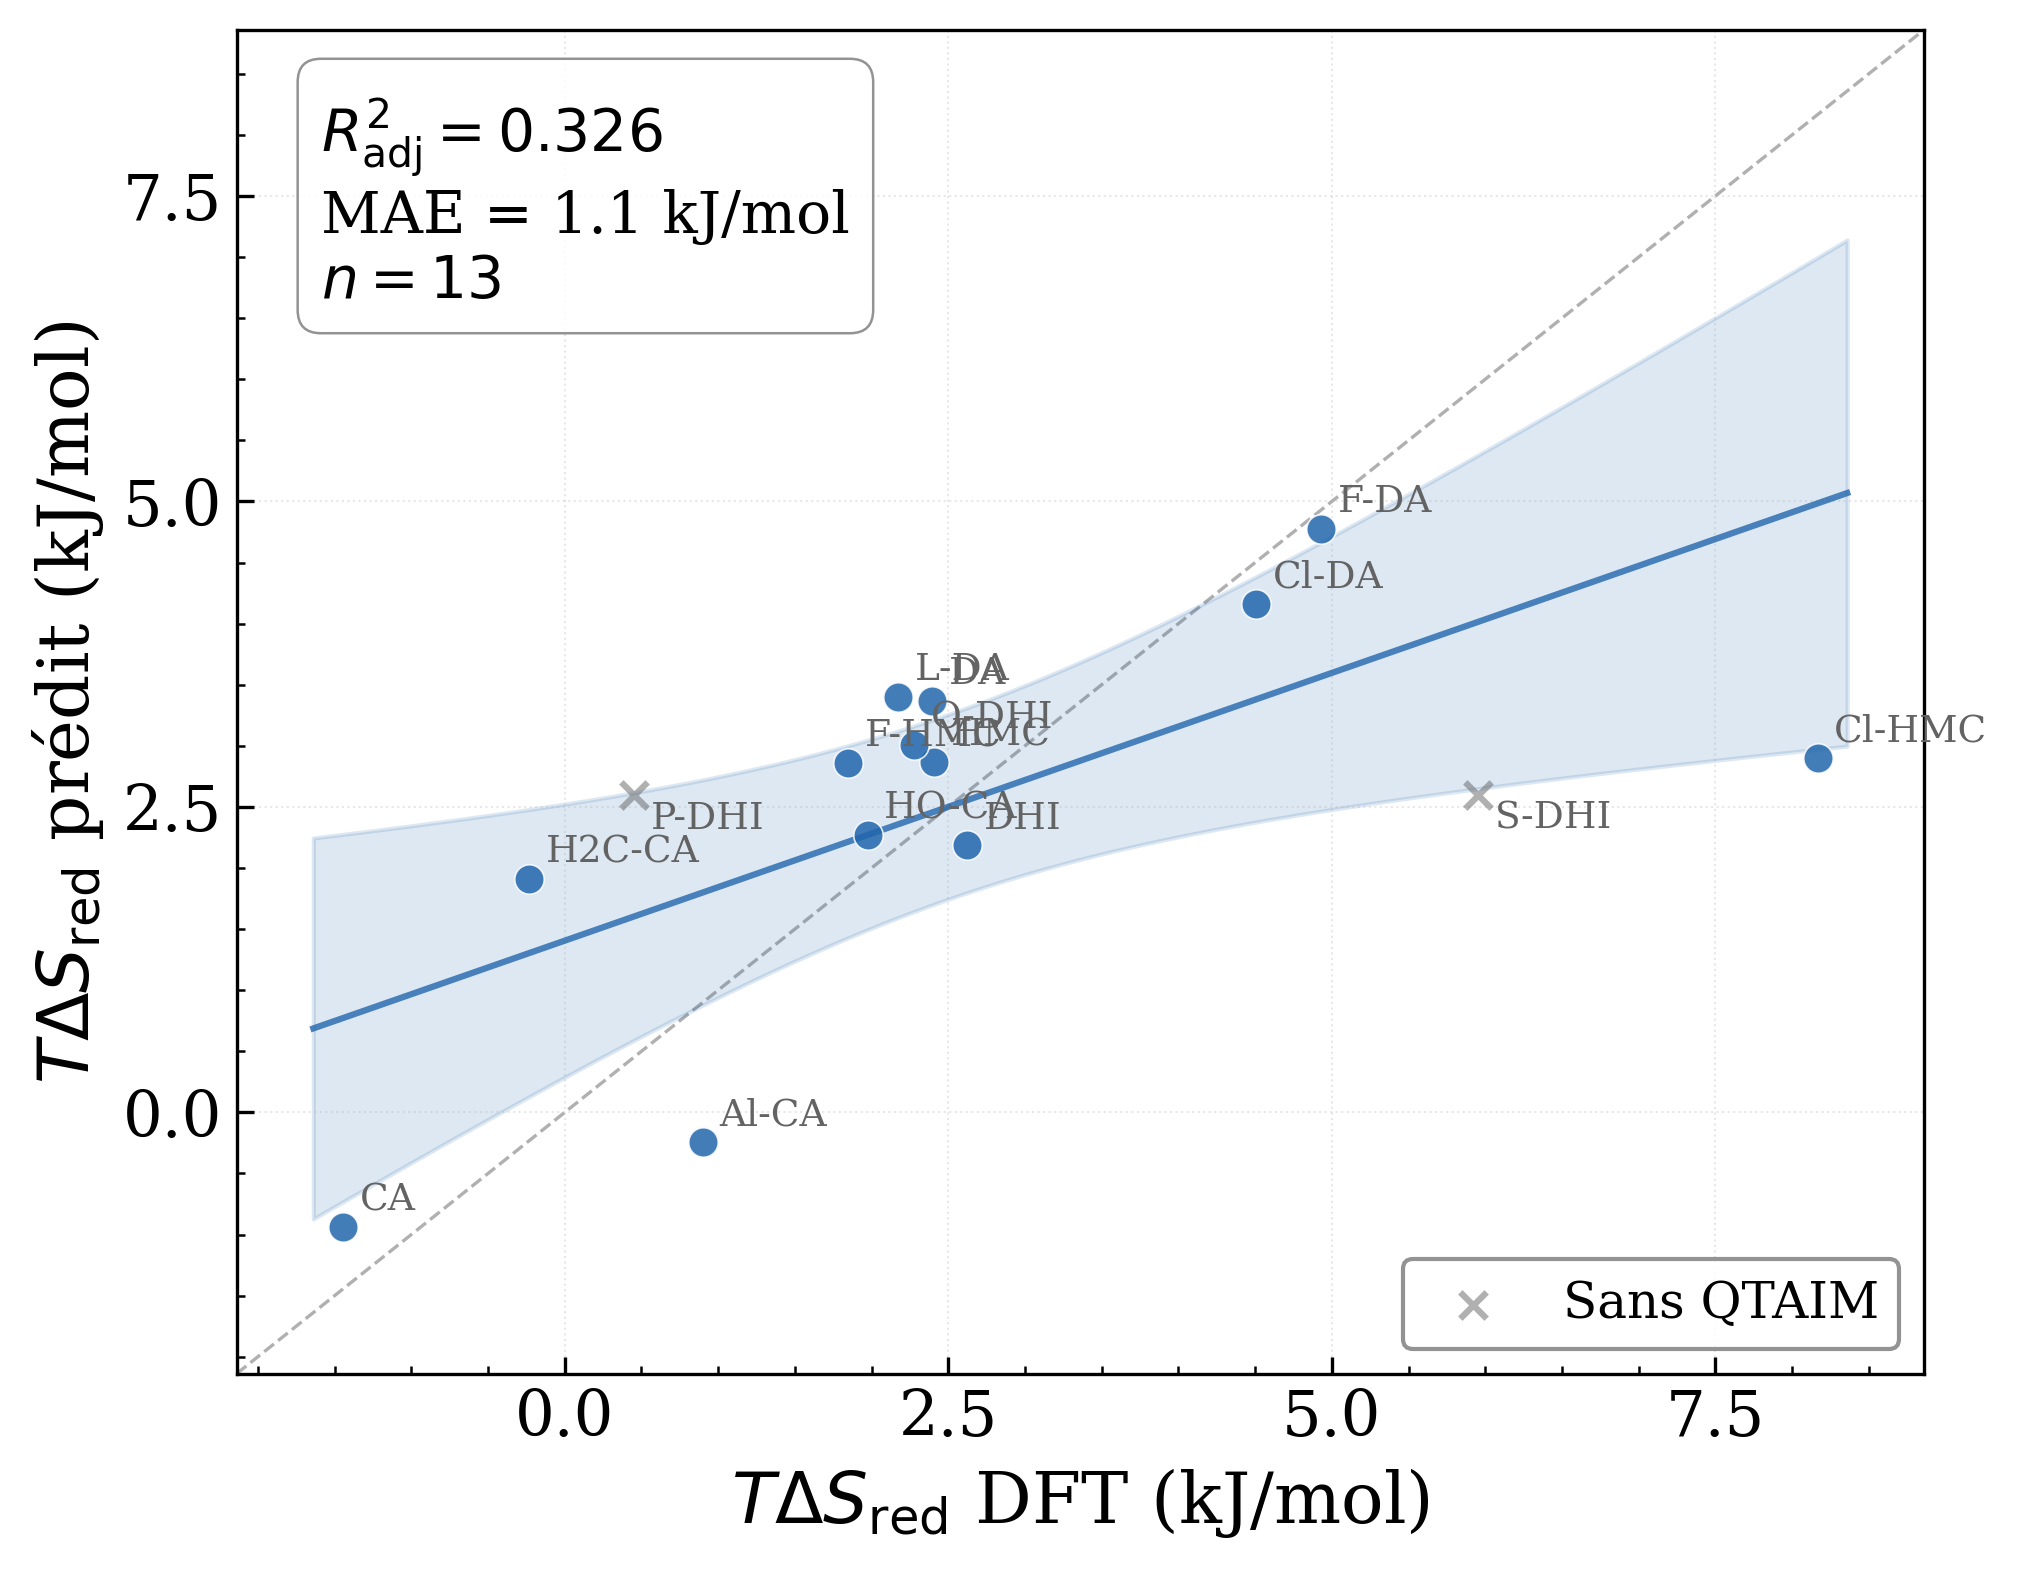
\includegraphics[width=\textwidth]{thermodynamic_models/TdS_bader_mu_red.png}
\caption{Réduction.}
\label{fig:tds_bader_red}
\end{subfigure}
\caption{Parity plots pour $T\Delta S$ : modèle bilinéaire $(\text{bader}_{\text{sumO}}, \mu)$ vs valeurs DFT de référence. La diagonale $y = x$ (pointillés) représente la prédiction parfaite. Les croix grises indiquent les molécules sans descripteurs QTAIM (P-DHI, S-DHI), pour lesquelles le modèle constant est utilisé.}
\label{fig:tds_bader}
\end{figure}

L'amélioration plus marquée en réduction qu'en oxydation est cohérente avec la plus grande variance de $T\Delta S_{\text{red}}$ ($\sigma = \SI{2.5}{kJ/mol}$ vs $\SI{1.1}{kJ/mol}$ en oxydation), qui offre davantage de signal à capturer. Notons que le $R^2_{\text{adj}}$ reste modeste malgré le gain en MAE : le modèle corrige les outliers (molécules à fort $T\Delta S$) sans capturer parfaitement les variations fines.

%-----------------------------------------------------------------------
\subsection{Prédiction combinée de $\Delta G^\circ$}
\label{sec:dG_combined}

L'objectif est de prédire $\Delta G^\circ$ à partir d'un seul calcul DFT sur l'état neutre (optimisation géométrique + modes normaux + single-point ionique), sans optimiser la géométrie ionique. La décomposition thermodynamique s'écrit :
\begin{align}
\Delta G_{\text{ox}} &= \text{IP} + E_{\text{relax}}^{\text{ox}} + \Delta\Delta U_{\text{ox}} - T\Delta S_{\text{ox}} \label{eq:dG_ox_decomp} \\
\Delta G_{\text{red}} &= -\text{EA} + E_{\text{relax}}^{\text{red}} + \Delta\Delta U_{\text{red}} - T\Delta S_{\text{red}} \label{eq:dG_red_decomp}
\end{align}

Chaque composante est prédite par le modèle le plus adapté :

\begin{table}[H]
\centering
\caption{Modèles prédictifs par composante de $\Delta G^\circ$, validés end-to-end sur $n = 13$ molécules disposant de données predict-dg. MAE en kJ/mol.}
\label{tab:component_models}
\footnotesize
\begin{tabular}{llcc}
\toprule
\textbf{Composante} & \textbf{Modèle} & \textbf{MAE (ox)} & \textbf{MAE (red)} \\
\midrule
EA / IP & Koopmans ($\varepsilon_{\text{HOMO/LUMO}}$, fit linéaire) & 2.6 & 2.2 \\
$E_{\text{relax}}$ & LVC2 calibré & 1.8 & 3.5 \\
$\Delta\Delta U$ & Constant (ox) / $\eta$ linéaire (red, éq.~\ref{eq:ddU_red_eta}) & 0.5 & 0.8 \\
$T\Delta S$ & Bilinéaire (bader$_{\text{sumO}}$, $\mu$) (éqs.~\ref{eq:tds_red_bader}--\ref{eq:tds_ox_bader}) & 0.8 & 1.1 \\
\midrule
$\Delta G^\circ$ & Combiné & 5.5 & 6.7 \\
\bottomrule
\end{tabular}
\end{table}

\paragraph{Résultats.}
La figure~\ref{fig:dG_parity} montre les parity plots $\Delta G^\circ_{\text{DFT}}$ vs $\Delta G^\circ_{\text{prédit}}$.

\begin{figure}[H]
\centering
\begin{subfigure}[t]{0.42\textwidth}
\centering
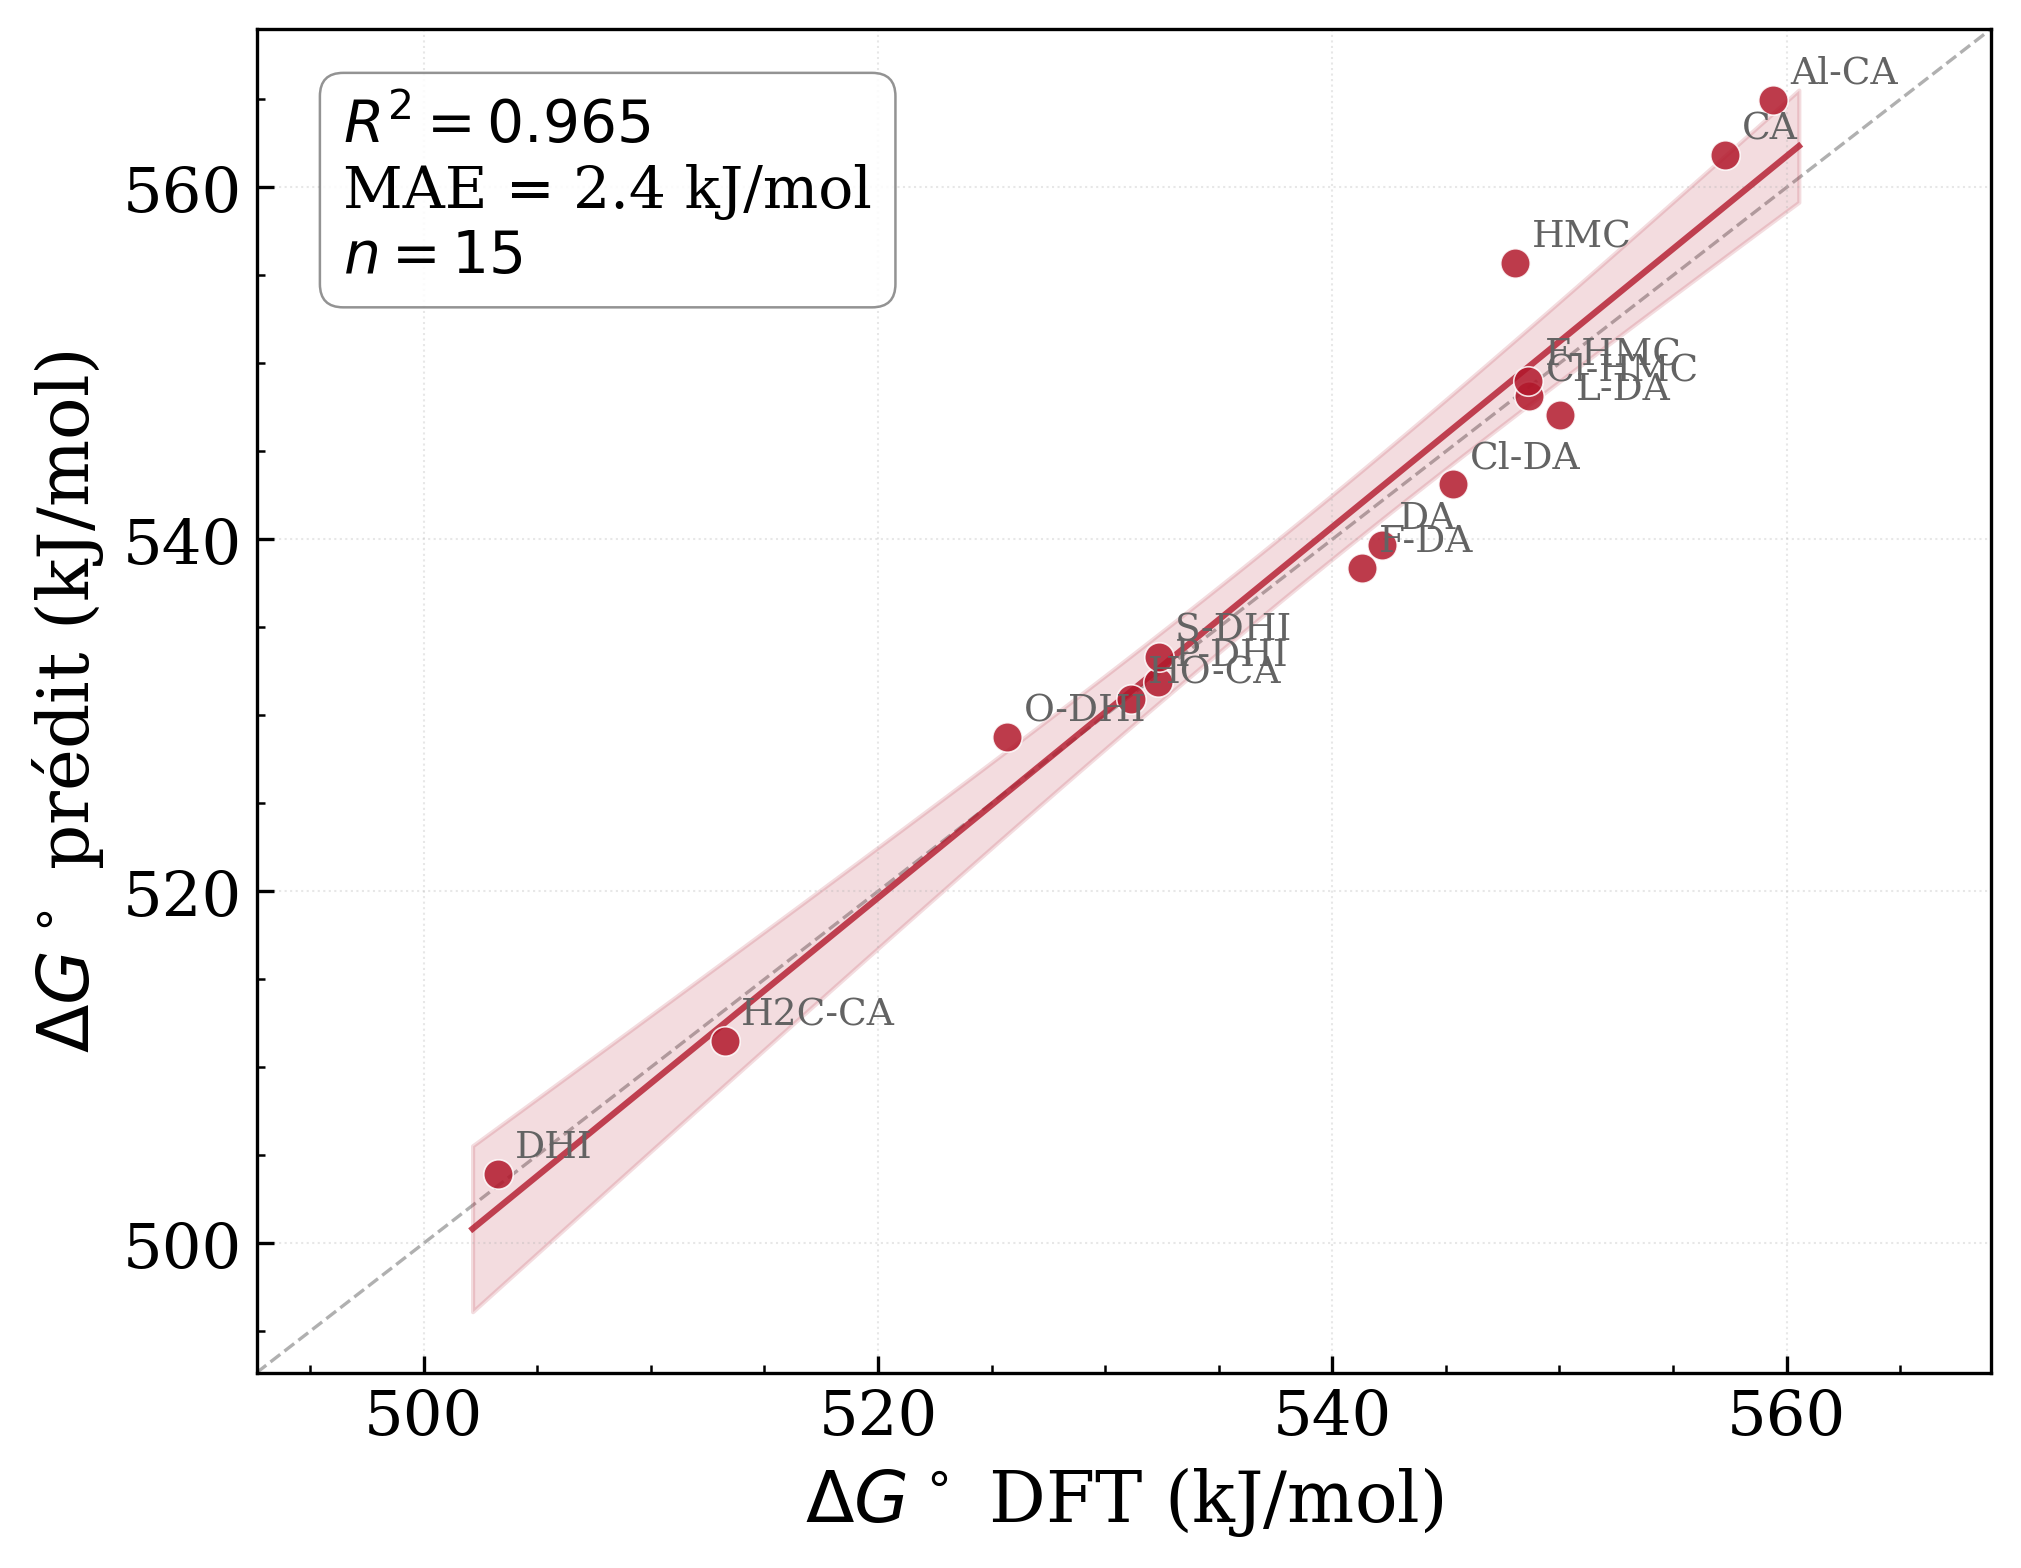
\includegraphics[width=\textwidth]{thermodynamic_models/dG_parity_ox.png}
\caption{Oxydation.}
\label{fig:dG_parity_ox}
\end{subfigure}
\hfill
\begin{subfigure}[t]{0.42\textwidth}
\centering
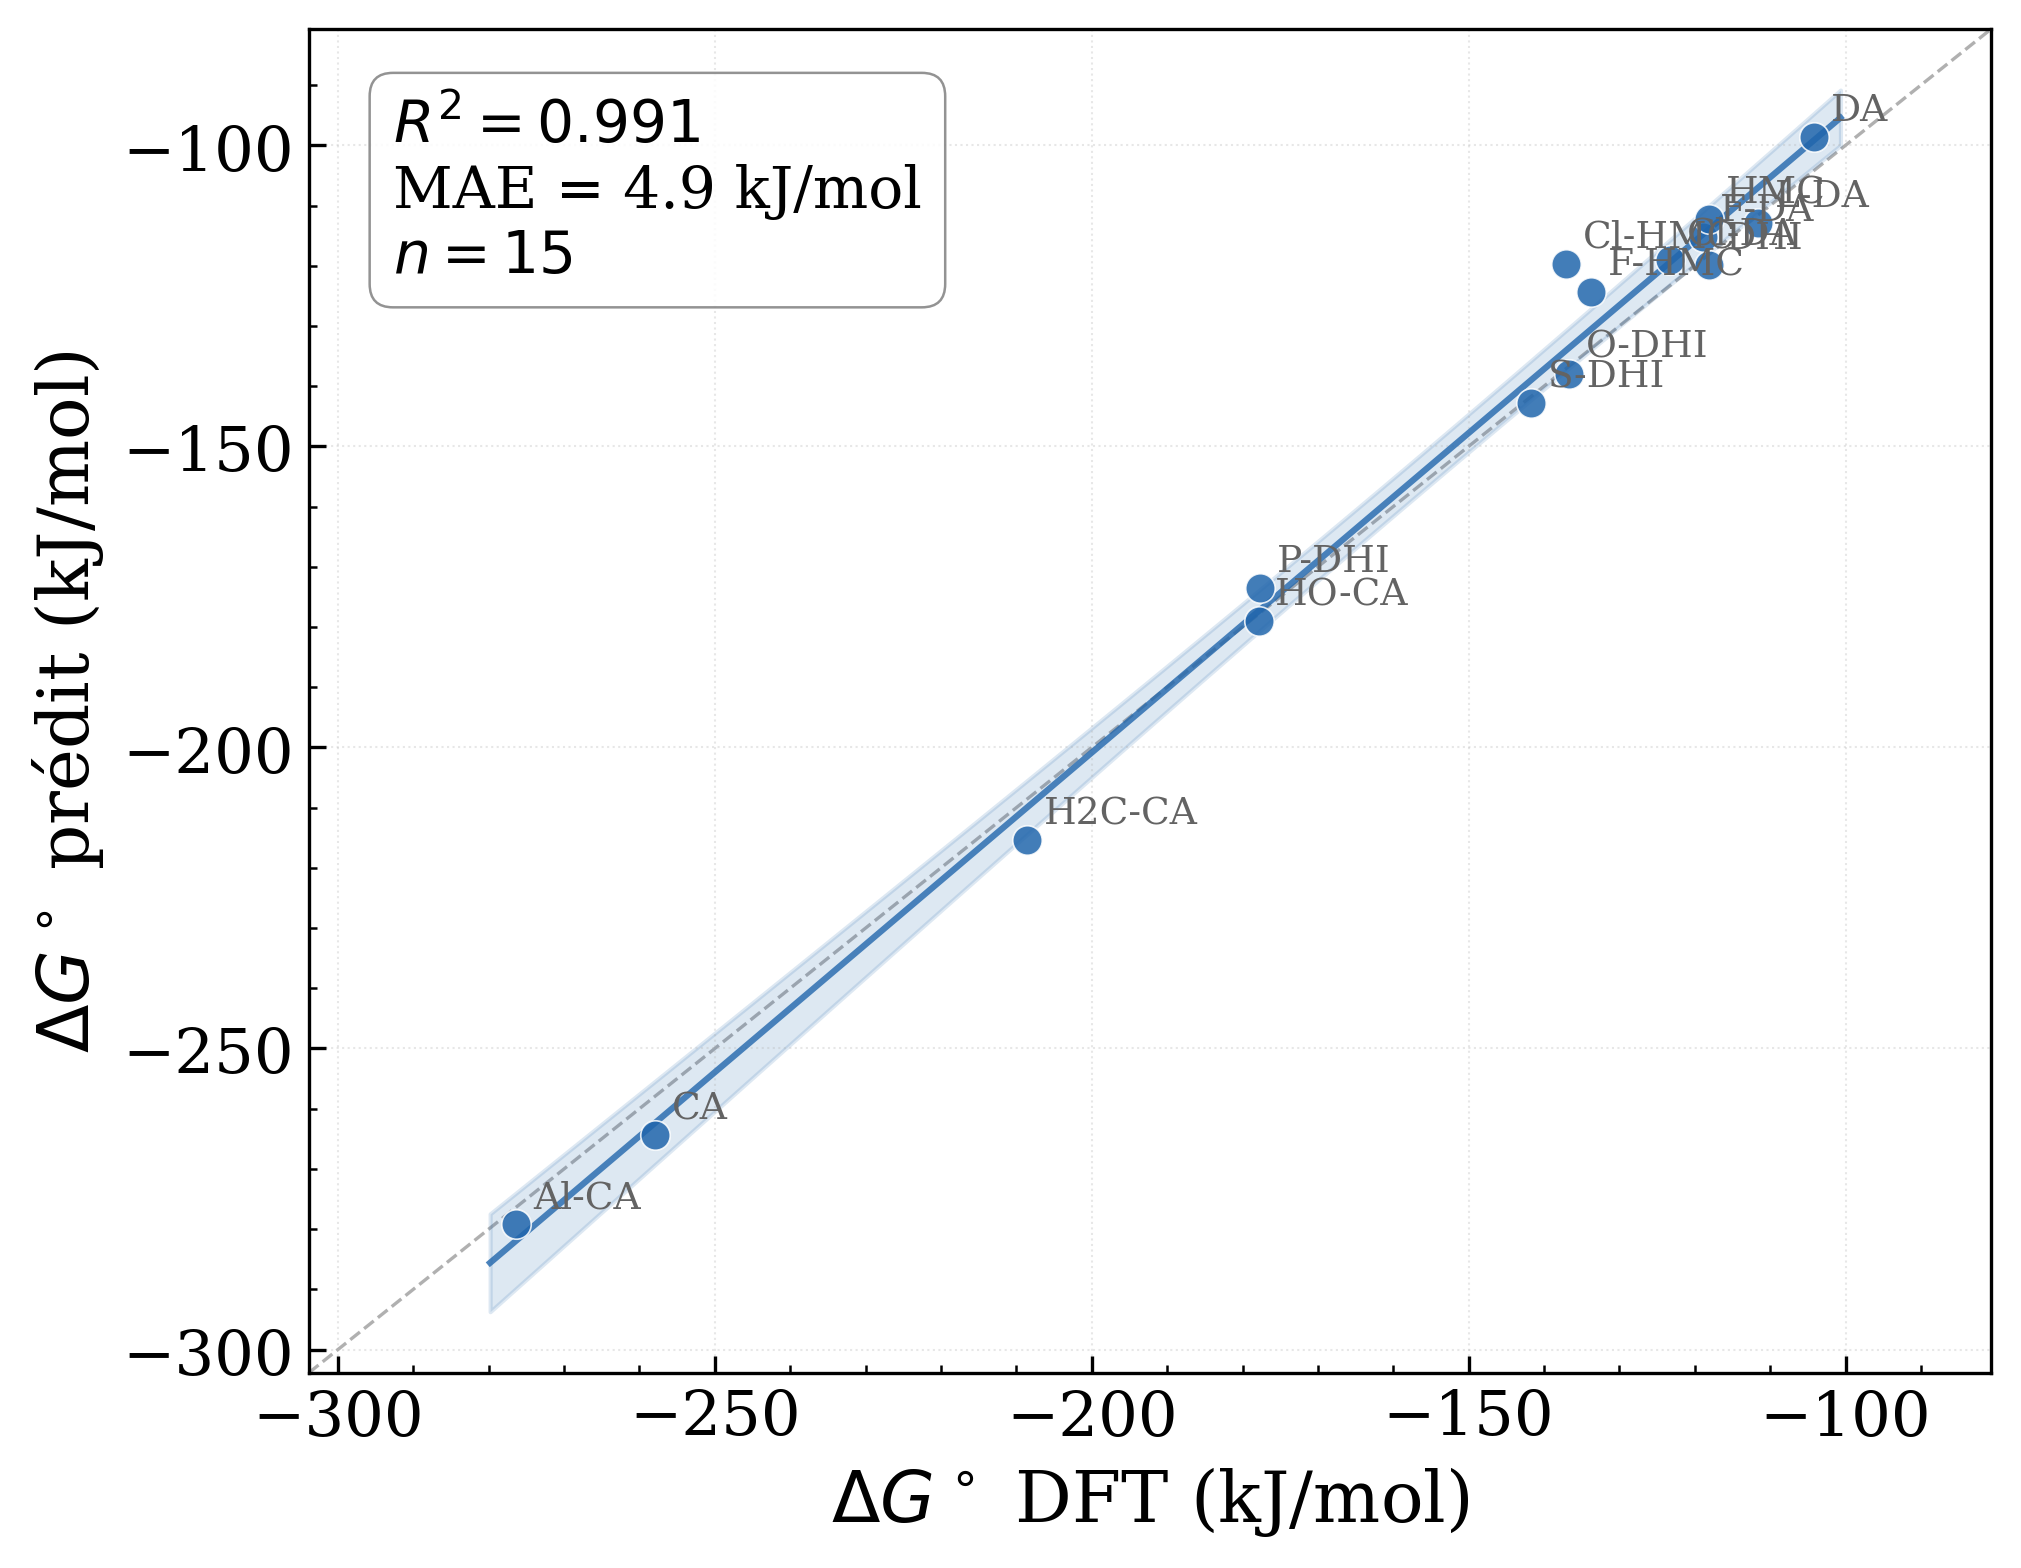
\includegraphics[width=\textwidth]{thermodynamic_models/dG_parity_red.png}
\caption{Réduction.}
\label{fig:dG_parity_red}
\end{subfigure}
\caption{Prédiction combinée de $\Delta G^\circ$. La diagonale $y = x$ (pointillés) représente la prédiction parfaite.}
\label{fig:dG_parity}
\end{figure}

\begin{itemize}[noitemsep]
\item \textbf{Oxydation} : MAE $= \SI{5.5}{kJ/mol}$ ($R^2 = 0.84$, $n = 13$). L'erreur est dominée par les composantes EA/IP (Koopmans, MAE $= \SI{2.6}{kJ/mol}$) et $E_{\text{relax}}$ (LVC2, MAE $= \SI{1.8}{kJ/mol}$).
\item \textbf{Réduction} : MAE $= \SI{6.7}{kJ/mol}$ ($R^2 = 0.97$, $n = 13$). Le goulot d'étranglement est ici $E_{\text{relax}}^{\text{red}}$ (MAE $= \SI{3.5}{kJ/mol}$), qui reflète la difficulté du LVC2 à capturer les réarrangements conformationnels importants. Les modèles améliorés de $\Delta\Delta U$ et $T\Delta S$ apportent un gain modeste sur $\Delta G^\circ$ combiné ($\SI{6.9}{} \to \SI{6.7}{kJ/mol}$) car les erreurs des composantes se compensent partiellement dans la somme.
\item \textbf{Budget d'erreur} : le remplacement du modèle constant par $\eta$ pour $\Delta\Delta U_{\text{red}}$ divise la MAE composante par 2.3 (\SI{1.7}{} $\to$ \SI{0.8}{kJ/mol}), ce qui représente le gain individuel le plus important. L'amélioration est néanmoins diluée par les erreurs dominantes d'EA/IP et $E_{\text{relax}}$.
\end{itemize}

\paragraph{Score de confiance.}
Le RMSD de réorganisation structurale constitue le meilleur discriminant de la fiabilité de la prédiction. Le tableau~\ref{tab:confidence_tiers} définit les niveaux de confiance correspondants.

\begin{table}[H]
\centering
\caption{Niveaux de confiance pour la prédiction de $\Delta G^\circ_{\text{red}}$ selon le RMSD de réorganisation.}
\label{tab:confidence_tiers}
\footnotesize
\begin{tabular}{llccc}
\toprule
\textbf{Tier} & \textbf{Critère RMSD} & $\boldsymbol{n}$ & \textbf{MAE $\Delta G^\circ$} & \textbf{Max$|$err$|$} \\
\midrule
Élevé & RMSD $< \SI{0.15}{\angstrom}$ & 3 & \SI{4.5}{kJ/mol} & \SI{6.9}{kJ/mol} \\
Modéré & $\SI{0.15}{\angstrom} \leq$ RMSD $< \SI{0.30}{\angstrom}$ & 5 & \SI{12.1}{kJ/mol} & \SI{16.5}{kJ/mol} \\
Bas & RMSD $\geq \SI{0.30}{\angstrom}$ & 3 & \SI{23.9}{kJ/mol} & \SI{36.1}{kJ/mol} \\
\bottomrule
\end{tabular}
\end{table}

Pour le tier élevé (RMSD $< \SI{0.15}{\angstrom}$, soit 3 molécules : H2C-CA, CA, Al-CA), la prédiction est bonne (MAE $= \SI{3.3}{kJ/mol}$). Le tier modéré (5 molécules : DHI, Cl-DA, HMC, DA, F-DA) présente une MAE de \SI{12.1}{kJ/mol}. Le tier bas (3 molécules : F-HMC, Cl-HMC, HO-CA) correspond à des réarrangements conformationnels significatifs (RMSD $\geq \SI{0.30}{\angstrom}$), où le résidu anharmonique non capté par le LVC2 dégrade la prédiction (MAE $= \SI{23.9}{kJ/mol}$).

\paragraph{Bilan.}
Le protocole de criblage rapide fonctionne pour les deux processus : un seul calcul DFT sur l'état neutre (optimisation + modes normaux) suivi d'un single-point ionique (avec NormalModes, DFT conceptuelle et QTAIM) permet de prédire $\Delta G^\circ$ avec une MAE de \SI{5.5}{kJ/mol} en oxydation et \SI{6.7}{kJ/mol} en réduction ($n = 13$), réduisant le coût computationnel d'un facteur~$\sim$5. Les modèles CDFT/QTAIM améliorent la prédiction composante par composante (facteur 2.3 pour $\Delta\Delta U_{\text{red}}$), mais l'impact sur $\Delta G^\circ$ combiné reste modeste du fait des compensations d'erreurs entre composantes et de la précision limitante de $E_{\text{relax}}^{\text{red}}$ pour les molécules à forte réorganisation structurale.

